% \documentclass{article}



% % if you need to pass options to natbib, use, e.g.:
%     \PassOptionsToPackage{numbers, compress}{natbib}
% before loading neurips_data_2023

% ready for submission
% \usepackage{neurips_data_2023}
\usepackage[preprint]{neurips_data_2023}

% to compile a preprint version, add the [preprint] option, e.g.:
%     \usepackage[preprint]{neurips_data_2023}
% This will indicate that the work is currently under review.

% to compile a camera-ready version, add the [final] option, e.g.:
%     \usepackage[final]{neurips_data_2023}

% to avoid loading the natbib package, add option nonatbib:
%    \usepackage[nonatbib]{neurips_data_2023}

% Submissions to the datasets and benchmarks are typically non anonymous,
% but anonymous submissions are allowed. If you feel that you must submit 
% anonymously, you can compile an anonymous version by adding the [anonymous] 
% option, e.g.:
%     \usepackage[anonymous]{neurips_data_2023}
% This will hide all author names.

\usepackage{color}
\usepackage{soul}
\usepackage[dvipsnames]{xcolor}
\usepackage[normalem]{ulem}
\newcommand{\todo}[1]{\textcolor{BrickRed}{[\textbf{TODO}]} }
\newcommand{\tocite}[1]{\textcolor{Plum}{[\textbf{CITE}: #1]}}
\newcommand{\hlc}[2][yellow]{{%
    \colorlet{foo}{#1}%
    \sethlcolor{foo}\hl{#2}}%
}
\newcommand{\tofix}[1]{\hlc[red!20]{#1}}

\usepackage[utf8]{inputenc} % allow utf-8 input
\usepackage[T1]{fontenc}    % use 8-bit T1 fonts
\usepackage{hyperref}       % hyperlinks
\usepackage{url}            % simple URL typesetting
\usepackage{booktabs}       % professional-quality tables
\usepackage{nicefrac}       % compact symbols for 1/2, etc.
\usepackage{microtype}      % microtypography
\usepackage{xcolor}         % colors
\usepackage{multirow}
\usepackage{graphicx}

%% MATH PACKAGES
\usepackage{amsfonts}       % blackboard math symbols
\usepackage{amsmath}
\usepackage{nicefrac} 


\usepackage{listings}
% \usepackage{minted}
% \usepackage[cachedir=.]{minted}
% \usepackage{frozencache}
% \usepackage[frozencache=true,cachedir=minted]{minted} 
\usepackage[finalizecache=true,cachedir=minted-cache]{minted}
% \usepackage[cachedir=.]{minted}

% \usepackage{appendix}

% here is a macro expanding to the name of the language
% (handy if you decide to change it further down the road)

% \newcommand\YAMLcolonstyle{\color{red}\mdseries}
\newcommand\YAMLkeystyle{\color{black}\bfseries}
\newcommand\YAMLvaluestyle{\color{blue}\mdseries}

\makeatletter

% here is a macro expanding to the name of the language
% (handy if you decide to change it further down the road)
\newcommand\language@yaml{yaml}

\expandafter\expandafter\expandafter\lstdefinelanguage
\expandafter{\language@yaml}
{
  keywords={true,false,null,y,n},
  keywordstyle=\color{darkgray}\bfseries,
  basicstyle=\YAMLkeystyle,                                 % assuming a key comes first
  sensitive=false,
  comment=[l]{\#},
  morecomment=[s]{/*}{*/},
  commentstyle=\color{purple}\ttfamily,
  stringstyle=\YAMLvaluestyle\ttfamily,
  moredelim=[l][\color{orange}]{\&},
  moredelim=[l][\color{magenta}]{*},
  moredelim=**[il][\YAMLcolonstyle{:}\YAMLvaluestyle]{:},   % switch to value style at :
  morestring=[b]',
  morestring=[b]",
  literate =    {---}{{\ProcessThreeDashes}}3
                {>}{{\textcolor{red}\textgreater}}1     
                {|}{{\textcolor{red}\textbar}}1 
                {\ -\ }{{\mdseries\ -\ }}3,
}

% switch to key style at EOL
\lst@AddToHook{EveryLine}{\ifx\lst@language\language@yaml\YAMLkeystyle\fi}
\makeatother

\newcommand\ProcessThreeDashes{\llap{\color{cyan}\mdseries-{-}-}}


\definecolor{codegreen}{rgb}{0,0.6,0}
\definecolor{codegray}{rgb}{0.5,0.5,0.5}
\definecolor{codepurple}{rgb}{0.58,0,0.82}
\definecolor{backcolour}{rgb}{0.95,0.95,0.92}

\lstdefinestyle{pythonstyle}{
    % backgroundcolor=\color{backcolour},   
    commentstyle=\color{codegreen},
    keywordstyle=\color{magenta},
    numberstyle=\tiny\color{codegray},
    stringstyle=\color{codepurple},
    basicstyle=\ttfamily\footnotesize,
    breakatwhitespace=false,         
    breaklines=true,                 
    captionpos=b,                    
    keepspaces=true,                 
    numbers=left,                    
    numbersep=5pt,                  
    showspaces=false,                
    showstringspaces=false,
    showtabs=false,                  
    tabsize=2
}

\lstset{style=pythonstyle}


% \title{\textsc{OceanBench}: \\ The Sea Surface Height Edition}

% % % The \author macro works with any number of authors. There are two commands
% used to separate the names and addresses of multiple authors: \And and \AND.
%
% Using \And between authors leaves it to LaTeX to determine where to break the
% lines. Using \AND forces a line break at that point. So, if LaTeX puts 3 of 4
% authors names on the first line, and the last on the second line, try using
% \AND instead of \And before the third author name.

\author{%
  J. Emmanuel Johnson$^*$\\
%   MEOM/Institut des Géosciences de l’Environnement, UGA\\
  % Univ. Grenoble Alpes, CNRS UMR IGE, Grenoble, France\\
  CNRS UMR IGE \\
  \texttt{johnsonj@univ-grenoble-alpes.fr}\\
  % examples of more authors
  \And
  Quentin Febvre$^*$\\
  IMT Atlantique\\
  \texttt{quentin.febvre@imt-atlantique.fr} \\
  \And
  Anastasia Gorbunova\\
  CNRS UMR IGE \\
  % \texttt{gorbunoa@univ-grenoble-alpes.fr} \\
  \And
  Sammy Metref\\
  DATLAS\\
  % \texttt{metrefs@univ-grenoble-alpes.fr}\\
  \And
  Maxime Ballarotta\\
  CLS\\
  % \texttt{mballarotta@groupcls.com} \\
  \And
  Julien Le Sommer\\
  CNRS UMR IGE\\
  % \texttt{julien.lesommer@univ-grenoble-alpes.fr} \\
  \And
  Ronan Fablet\\
  IMT Atlantique \\
  % \texttt{ronan.fablet@imt-atlantique.fr} \\
}


% \author{%
%   David S.~Hippocampus\thanks{Use footnote for providing further information
%     about author (webpage, alternative address)---\emph{not} for acknowledging
%     funding agencies.} \\
%   Department of Computer Science\\
%   Cranberry-Lemon University\\
%   Pittsburgh, PA 15213 \\
%   \texttt{hippo@cs.cranberry-lemon.edu} \\
%   % examples of more authors
%   % \And
%   % Coauthor \\
%   % Affiliation \\
%   % Address \\
%   % \texttt{email} \\
%   % \AND
%   % Coauthor \\
%   % Affiliation \\
%   % Address \\
%   % \texttt{email} \\
%   % \And
%   % Coauthor \\
%   % Affiliation \\
%   % Address \\
%   % \texttt{email} \\
%   % \And
%   % Coauthor \\
%   % Affiliation \\
%   % Address \\
%   % \texttt{email} \\
% }


% \begin{document}




% \maketitle
% \def\thefootnote{*}\footnotetext{These authors contributed equally to this work}\def\thefootnote{\arabic{footnote}}
\begin{bibunit}[IEEEtran.bst]

\chapter{\textsc{OceanBench}: The Sea Surface Height Edition}
% \addcontentsline{toc}{chapter}{\textsc{OceanBench}: The Sea Surface Height Edition}
\chaptermark{\textsc{OceanBench}: The Sea Surface Height Edition}
%##################################
% KEYWORDS
% - Sea Surface Height
% - Interpolation
% - Inverse Problem
% - 
% Scientific Machine Learning
% Benchmark, Partial Differential Equations, PINN, FNO, U-Net, Inverse problem
% \linenumbers
% % \begin{abstract}
% The ocean is a key component of the climate system, profoundly influencing human activities. Consequently, a central question for oceanographers revolves around its observation and prediction at different timescales. Similar to various research fields, oceanography has recently witnessed the emergence of machine learning-based methods as an alternative to more domain-specific approaches. But, surprisingly, the adoption of machine learning methods in this field has been arguably slower compared to others. This can be attributed to the complexity of pre-processing tasks in the domain of geospatial data and to the specialized nature of evaluation metrics relevant to ocean science problems. In this context, we introduce \texttt{OceanBench}, a framework designed to lower the barrier to entry for ML researchers by standardizing and automating this process that comply with domain-expert standards.
% It seeks to maintains readability, robustness, and flexibility by providing a standardized framework to explicitly highlight the preprocessing step used, the parameters chosen and the sequence of operations performed. 
% It takes a step towards incorporate these domain-driven decisions to integrate well with existing ML pipelines.
% We demonstrate the usefulness of \texttt{OceanBench} on a series of SSH interpolation tasks with consistent dataflow pipelines, physically-inspired metrics, and interpretable visualizations.

% \end{abstract}

  % The abstract paragraph should be indented \nicefrac{1}{2}~inch (3~picas) on
  % both the left- and right-hand margins. Use 10~point type, with a vertical
  % spacing (leading) of 11~points.  The word \textbf{Abstract} must be centered,
  % bold, and in point size 12. Two line spaces precede the abstract. The abstract
  % must be limited to one paragraph.

\begin{abstract}

The ocean is a crucial component of the Earth's system. 
It profoundly influences human activities and plays a critical role in climate regulation. 
Our understanding has significantly improved over the last decades with the advent of satellite remote sensing data, allowing us to capture essential sea surface quantities over the globe, e.g., sea surface height (SSH). 
Despite their ever-increasing abundance, ocean satellite data presents challenges for information extraction due to their sparsity and irregular sampling, signal complexity, and noise. 
Machine learning (ML) techniques have demonstrated their capabilities in dealing with large-scale, complex signals. 
Therefore we see an opportunity for these ML models to harness the full extent of the information contained in ocean satellite data. 
However, data representation and relevant evaluation metrics can be \textit{the} defining factors when determining the success of applied ML. 
The processing steps from the raw observation data to a ML-ready state and from model outputs to interpretable quantities require domain expertise, which can be a significant barrier to entry for ML researchers. 
In addition, imposing fixed processing steps, like committing to specific variables, regions, and geometries, will narrow the scope of ML models and their potential impact on real-world applications. 
\textbf{OceanBench} is a unifying framework that provides standardized processing steps that comply with domain-expert standards. 
It is designed with a flexible and pedagogical abstraction: it a) provides plug-and-play data and pre-configured pipelines for ML researchers to benchmark their models w.r.t. ML and domain-related baselines and b) provides a transparent and configurable framework for researchers to customize and extend the pipeline for their tasks. 
In this work, we demonstrate the \texttt{OceanBench} framework through a first edition dedicated to SSH interpolation challenges. 
We provide datasets and ML-ready benchmarking pipelines for the long-standing problem of interpolating observations from simulated ocean satellite data, multi-modal and multi-sensor fusion issues, and transfer-learning to real ocean satellite observations. 
The \texttt{OceanBench} framework is available at~\href{https://github.com/jejjohnson/oceanbench}{github.com/jejjohnson/oceanbench} and the dataset registry is available at~\href{https://github.com/quentinf00/oceanbench-data-registry}{github.com/quentinf00/oceanbench-data-registry}.

\end{abstract}


%%%%%%%%%%%%%%%%%%%%%%%%%%%%%%%%%%%%%%%%%%%%%%%%%%%%%%%%%%%%%%%%%%%%%%%%%%%%%%%%%%%%%%%%%%%%%%%%%%%%%%%%%%%%%%%%%%%%%%%%%%%%%%%%%%%%%%%%%%%%%%%%%

% - We demonstrate how \texttt{OceanBench} can be used as an underlying framework with a series of SSH interpolation tasks which combines different variables, regions and geometries. 


% Q - make use of everything we mentioned above!
% E/Q - we want to showcase that OceanBench can be used for SSH interpolation 
% - we want to demonstrate how we can design different experiments/modifications with minimal code changes
% Q - simple tasks SSH -> SSH; extend it a) add domain, b) include other variables, c) switching to real data
% - enrich a simple experimental setups with additional variations

%%%%%%%%%%%%%%%%%%%%%%%%%%%%%%%%%%%%%%%%%%%%%%%%%%%%%%%%%%%%%%%%%%%%%%%%%%%%%%%%%%%%%%%%%%%%%%%%%%%%%%%%%%%%%%%%%%%%%%%%%%%%%%%%%%%%%%%%%%%%%%%%%



%%%%%%%%%%%%%%%%%%%%%%%%%%%%%%%%%%%%%%%%%%%%%%%%%%%%%%%%%%%%%%%%%%%%%%%%%%%%%%%%%%%%%%%%%%%%%%%%%%%%%%%%%%%%%%%%%%%%%%%%%%%%%%%%%%%%%%%%%%%%%%%%%

% - There is some work to be done to get the observation data to a ML-ready state.
% - Deciding the appropriate transformations requires domain-expertise which can be a large barrier to entry for ML researchers.

% - ML methods cannot be applied out of the box on raw observation data because .. blah blah

% - Despite the potential of machine learning to solve the issues that plague geosciences, the barrier to entry for machine learning (ML) researchers in ocean sciences is often hindered by the vastly different schemes for preprocessing techniques required to get the geo-centric data to a ML-ready state.
% \texttt{OceanBench} is a framework for co-designing machine learning-driven high level data products from ocean observations. 
%%%%%%%%%
% Why dont we just provide the processed data and call it a day...?
% Q - 1) non-standardized preprocessing steps; 2) regional differences
% 1 - multiple ways to take advantage of the Obs data (covariates, coordinate-based, gridded)
% Keeping the flexibilities allow for extensibility and multiple 
%%%%%%%%%%%%$
% 1 - OceanBench is a unifying framework that provides standardized processing steps that comply with domain-expert standards.
% 2 - It is designed for - flexible, padagological, abstract, :
% a - getting ML researchers quickly involved (data + preconfigured pipelines -> ML ready setups and test their models)
% - provides data and preconfigured pipelines for ML researchers to quickly experiment with different setups,
% - transparent and configurable for researchers to customize and extend the pipeline for their own objectives
% b - pedagological, unified setup to create and modified tasks (extensible)
% - flexibility
% 3 - We demonstrate ho
% %
% \texttt{OceanBench} is a framework that standardizing ... these processing steps that comply with domain-expert standards.
% %
% It is designed to lower the barrier to entry for ML researchers by providing preconfigured pipelines, ... "one-stop-shop for it all", and providing illustrative examples for different audiences.
% * 
% * provide a common interface for the processing steps
% * create a few ML tasks from raw data to ML ready using the above steps
% * showcase how one can orchestrate preconfigured pipelines to create a variety of ML tasks
% * preconfigured pipelines to illustrate example applications

% 1 - getting ML researchers quickly involved (data + preconfigured pipelines -> ML ready setups and test their models)
% 2 - pedagological, unified setup to create and modified tasks

% %%%%%
% \texttt{OceanBench} is a framework 
% - lower the barrier to entry
% - accessibility
% - one place to look to get all the stuff you want to do
% - preconfigured pipelines
% - jbooks with illustrated examples.
% - standardized preprocessing steps.
%
% It seeks to maintains readability, robustness, and flexibility by providing a standardized framework to explicitly highlight the preprocessing step used, the parameters chosen and the sequence of operations performed. 
%
% It takes a step towards incorporate these domain-driven decisions to integrate well with existing ML pipelines.
%
% We demonstrate the usefulness of \texttt{OceanBench} on a series of SSH interpolation tasks with 
% consistent dataflow pipelines, physically-inspired metrics, and interpretable visualizations.


\section{Motivation}

The ocean is vital to the Earth's system~\cite{OCEANWARMING}. 
It plays a significant role in climate regulation regarding carbon~\cite{OCEANCARBONCYCLE} and heat uptake~\cite{OCEANHEATUPTAKE}. It is also a primary driver of human activities (e.g., maritime traffic and world trade, marine resources and services)~\cite{SSHOPERATIONAL, ML4OCN}. 
However, monitoring the ocean is a critical challenge: the ocean state can only partially be determined because most of the ocean consists of subsurface quantities that we cannot directly observe. 
Thus, to quantify even a fraction of the physical or biochemical ocean state, we must often rely only on surface quantities that we can monitor from space, drifting buoys, or autonomous devices.
Satellite remote sensing, in particular, is one of the most effective ways of measuring essential sea surface quantities~\cite{Altimetry} such as sea surface height (SSH)~\cite{DUACS}, sea surface temperature (SST)~\cite{OCEANSATELLITESST}, and ocean color (OC)~\cite{OCEANSATELLITEOC}. 
While these variables characterize only a tiny portion of the ocean ecosystem, they present a gateway to many other derived physical quantities~\cite{ML4OCN}.


% satellite-derived SSH data allow us to monitor the sea level rise as well as critical physical and biogeochemical ocean processes,
Although we can access observable sea surface quantities, they are generally irregularly and extremely sparsely sampled. 
For instance, satellite-derived SSH data has less than 5\% coverage of the globe daily~\cite{DUACS}. 
These sampling gaps make the characterization of ocean processes highly challenging for operational products and downstream tasks that depend on relevant gap-free variables. This has motivated a rich literature in geoscience over the last decades, mainly using geostatistical kriging methods \cite{DUACS, MIOST} and model-driven data assimilation schemes~\cite{BFNQG, GLORYS12}. Despite significant progress, these schemes often need to improve their ability to leverage available observation datasets' potential fully. 
This has naturally advocated for exploring data-driven approaches like shallow ML schemes~\cite{DINEOF, DINEOF2, ANALOGDA2, ANALOGDA}. Very recently, deep learning schemes \cite{SSHInterpAttention, SSHInterpConvLSTM, SSHInterpUNet} have become appealing solutions to benefit from existing large-scale observation and simulation datasets and reach significant breakthroughs in the monitoring of upper ocean dynamics from scarcely and irregularly sampled observations. However, the heterogeneity and characteristics of the observation data present major challenges for effectively applying these methods beyond idealized case studies. 
A data source could have different variables, geometries, and noise levels, resulting in many domain-specific preprocessing procedures that can vastly change the solution outcome.
Furthermore, the evaluation procedure of the methods and their effectiveness can be regionally-dependent as the physical phenomena vary in space and time, which adds another layer of complexity in convincing domain scientists of their trustworthiness.
So the entire ML pipeline now requires a unified framework for dealing with heterogeneous data sources, different pre- and post-processing methodologies, and regionally-dependent evaluation procedures.

 %So the nature of the observations presents a key challenge for operational products and downstream tasks that depend on relevant gap-free variables.
%In addition, this sparsity 
%Although methods like smoothers~\tocite{OI, MIOST}, data assimilation~\tocite{BFN} and machine learning (ML)~\tocite{NerFs,recent-stuff, Ronan} have produced viable solutions to filling the gaps in ocean satellite, the heterogeneity and characteristics of the observation data present major challenges for effectively applying these methods. 
% No model nor observation systems captures all scales and processes.
% Operational methods like optimal interpolation and data assimilation ...
% Thus, there is a need for better model/data integration schemes that fully benefit from HR models and ever-increasing observation datasets.

% \textbf{Opportunity}.
%An end-to-end framework for piping data from its raw form to an ML-ready state and from model outputs to interpretable quantities is challenging. Designing an effective system that does this is the basis for many MLOPs tools and research~\tocite{MLOPs Research}.
To address these challenges, we introduce \textbf{OceanBench}, a framework for co-designing machine-learning-driven high-level experiments from ocean observations. 
It consists of an end-to-end framework for piping data from its raw form to an ML-ready state and from model outputs to interpretable quantities. 
We regard \texttt{OceanBench} as a key facilitator for the uptake of MLOPs tools and research~\cite{MLOPS1,MLOPS2} for ocean-related datasets and case studies. This first edition provides datasets and ML-ready benchmarking pipelines for SSH interpolation problems, an essential topic for the space oceanography community, related to ML communities dealing with issues like in-painting~\cite{InPaintingSurvey}, denoising~\cite{DENOISESURVEY,DENOISESURVEY2}, and super-resolution~\cite{SuperResSurvey}. 
We expect \texttt{OceanBench} to facilitate new challenges to the applied machine learning community and contribute to meaningful ocean-relevant breakthroughs.
%
The remainder of the paper is organized as follows: in \S2, we outline some related work that was inspirational for this work; in \S3, we formally outline \texttt{OceanBench} by highlighting the target audience, code structure, and problem scope; in \S4, we outline the problem formulation of SSH interpolation and provide some insight into different tasks related to SSH interpolation where \texttt{OceanBench} could provide some helpful utility; and in \S5 we give some concluding remarks while also informally inviting other researchers to help fill in the gaps.

% \textbf{How We Measure SSH + Gap Problem}. 




% % \textbf{Data Deluge, Gaps, \& ML Integration}. 
% Like most geosciences, the ocean sciences also suffer from the data deluge that persists due to the large amounts of observed quantities being collected daily~\tocite{Gus}. 
% The increased availability and quantity of observations are beneficial because it offers the community more insight into the physical processes at a finer resolution.
% % Consequently, this can help oceanographers revolve a central question of observing and predicting the ocean state at different spatial and timescales. 
% The trade-off is that processing this data is very expensive.
% Furthermore, it is impossible to accurately measure the entire globe concurrently, resulting in data with many gaps.
% Many operational systems have historically used ad-hoc coordinate-based schemes to gap-fill the data based on covariance assumptions. 
% However, with the abundance of new data~\tocite{SWOT}, these covariance-based schemes are reaching their limit due to the computational and signal complexity.
% Machine learning (ML) has been recently introduced as a viable alternative to filling the gaps in data where many classes of methods have found success, including coordinate-based methods~\tocite{OI,MIOST,NerFs}, direct surrogate/hybrid methods~\tocite{BFN, recent-stuff}, and end-to-end learning schemes~\tocite{Ronan}. 
% Nevertheless, most of these methods have only been applied to regions, and more needs to be applied at a large scale that comes close to the operational settings.


% % \textbf{Logistics Problem}.
% % \textbf{The Problem with Observation Data}.
% % The community is quickly facing a logistics problem.
% Dealing with complex problems such as SSH interpolation requires dealing directly with the observation data, often involving aggregating observations from satellites, buoys, or autonomous devices.
% In all cases, we can only observe a tiny portion of the Earth at any given time, resulting in highly sparse data (often <5\% coverage).
% This problem is even more difficult because the data sources are often heterogeneous, with different variables, geometries, and noise levels.
% Furthermore, the evaluation procedure can be regionally dependent as the physical phenomena vary globally. 
% So the entire ML pipeline now requires a unified framework for dealing with heterogeneous data sources, different pre- and post-processing methodologies, and regional dependent evaluation procedures.

% To solve a difficult problem such as SSH interpolation requires a lot of interdisciplinary expertise including scientific, numerical and machine learning.
% To do effective ML research in this area, one needs a consistent \textit{pipeline} to funnel the data from its raw form through the transformations and to its evaluation state. 
% In standard ML research, we have copious amounts of \textit{datamodules} which encapsulate many underlying transformations procedures for many staple datasets, e.g. MNIST, CIFAR10, CELEB, etc.
% Even some weather and climate benchmark datasets have \cite{weatherbench,ClimateBench} access to gap-free, non-heterogenous reanalysis data.
% Despite the focus on the ML model in the current state of affairs, we have often found that the variables chosen and how they were preprocessed has the greatest effect on the final result.
% In previous benchmark settings~\citep{CHAOSBENCH,PDEBench,ClimateBench,weatherbench,ENS10Bench}, little attention was paid to the internals of the data preprocessing and this process was kept static.
% In geosciences, because we often deal with sparse, heterogeneous observations, we often need to decide and implement many crucial preprocessing transformations before we get to the modeling aspects.
% % including selecting regions, filtering, and calculating derived variables.
% As such, we should include the chosen variables and how they are preprocessed as hyperparameters to be optimized within the full ML pipeline.
% However, this complicates the entire pipeline because we have effectively compounded the complexity due to the many ways one can preprocess and modify the data in conjunction with decisions from the ML side like the architecture, the optimizer and the loss function.
% In addition, we may even have a large series of post-processing transformations which determine how we evaluate our models. Those transformations contain implementation details that may change between studies which make comparing and reproducing some results challenging.
% This results in a software engineering (SWE) roadblock which needs to be addressed should we wish to do effective research in applied ML research and this obstacle is especially prevalent in the geosciences.



% , through the transformations, into the model, and through the 
% Due to many of the many components needed to solve the problem it requires a pipeline. 
% For domain scientists, there is a lack of organization and ontology of previous ideas. 
% For machine learning researchers, ... 
% For downstream users, there is a lack of ontology of the current state of research which makes it difficult to readily apply these techniques for their problems.

% Nonetheless, most of this research has been done in parallel across disjoint sub-fields of research and to the best of our knowledge little to no work has been done on homogenising and integrating these distinct methods in a common framework



% In this paper, we wish to establish a well-defined software abstraction for dealing SSH interpolation using ML.
% Using ocean data is the primary goal which is a data assimilation problem. 
% However, there are many subsequent steps we need to improve. 1) We need gap-free data from the satellite observations, 2) we need surrogate or hybrid models to replace the expensive ocean models, and 3) we need end-to-end learning schemes to perform domain-specific tasks that incorporate good priors and the observations.

\section{Related Work}

Machine learning applied to geosciences is becoming increasingly popular, but there are few examples of transparent pipelines involving observation data. 
After a thorough literature review, we have divided the field into three camps of ML applications that pertain to this work: 1) toy simulation datasets, 2) reanalysis datasets, and 3) observation datasets. 
We outline the literature for each of the three categories below.

\textbf{Toy Simulation Data}. 
One set of benchmarks focuses on learning surrogate models for well-defined but chaotic dynamical systems in the form of ordinary differential equations (ODEs) and partial differential equations (PDEs) and there are freely available code bases which implement different ODEs/PDEs~\citep{CHAOSBENCH,PDEBench,pyQG,JAXCFD,NCARDART,NCARDARTSOFTWARE,VEROS,OCEANANIGANS}.
% For example, \texttt{Dyst} package~\cite{CHAOSBENCH} has many chaotic ODEs, and packages such as \texttt{PDEBench}~\cite{PDEBench}, pyQG~\citep{pyQG}, NCAR DART~\citep{NCARDART,NCARDARTSOFTWARE}, and jax-CFD~\citep{JAXCFD} have implementations of 2D/3D Spatial-Temporal PDEs similar to Navier-Stokes; 
This is a great testing ground for simple toy problems that better mimic the structures we see in real-world observations. 
% More ocean-related simulations include the pyQG package~\citep{pyQG}, the NCAR DART data assimilation testbed~\citep{NCARDART,NCARDARTSOFTWARE}.
Working with simulated data is excellent because it is logistically simple and allows users to test their ideas on toy problems without increasing the complexity when dealing with real-world data.
However, these are ultimately simple physical models that often do not reflect the authentic structures we see in real-world, observed data.

\textbf{Reanalysis Data}. 
This is assimilated data of real observations and model simulations. 
There are a few major platforms that host ocean reanalysis data like the Copernicus Marine Data Store~\citep{MDSOCEANPHYSICS,MDSBIOGEOCHEMICAL,MDSOCEANPHYSICSENS,MDSWAVES}, the Climate Data Store~\citep{CDSREANALYSISSST}, the BRAN2020 Model~\citep{DATABLUELINK}, and the NOAA platform~\citep{DATANCEP}. 
However, to our knowledge, there is no standard ML-specific ocean-related tasks to accompany the data. On the atmospheric side, platforms like \texttt{WeatherBench}~\cite{weatherbench}, \texttt{ClimateBench}~\cite{ClimateBench}, \texttt{ENS10}~\cite{ENS10Bench} were designed to assess short-term and medium-term forecasting using ML techniques with recent success of ML~\cite{GraphCast,FourCastNet}
% While the original papers featured straightforward methods, there has been swift subsequent development within the last few years~\cite{GraphCast,FourCastNet}. 
% Apart from industry momentum and investment, we attribute the recent adoption and success of ML to the problem's clarity, the original tasks' openness, and the software's ML compatibility. 
The clarity of the challenges set by the benchmark suites has inspired the idea of \texttt{OceanBench}, where we directly focus on problems dealing with ocean observation data.

\textbf{Observation Data}. 
These observation datasets (typically sparse) stem from satellite observations that measure surface variables or in-situ measurements that measure quantities within the water column. 
Some major platforms to host data include the Marine Data Store~\citep{MDSALONGTRACK,MDSINSITU}, the Climate Data Store~\citep{CDSOBSSST,CDSOBSSSTENS,CDSOBSOC}, ARGO~\citep{ARGO}, and the SOCAT platform~\citep{SOCAT}.
However, it is more difficult to assess the efficacy of operational ML methods that have been trained only on observation data and, to our knowledge, there is no coherent ML benchmarking system for ocean state estimation.
% In one community, there is the Surface Ocean CO$_2$ Atlas (SOCAT)~\cite{SOCAT} which is a community effort to aggregate all collocated observations (included SSH) which help predict the fugacity of carbon dioxide (fCO$_2$). 
% This has been a huge effort to provide a consistently updated suite of observations for some key variables that are important in biogeochemical processes.
% However, there is currently no coherent benchmarking system with standard metrics despite their being a wide range of new methods to try and tackle the interpolation problem.
% Most new work tends to use the observations provided with their own additional variable with no standard comparison framework other works.
% In a completely different community, 
There has been significant effort by the \textit{Ocean-Data-Challenge} Group\footnote{Ocean Data Challenge group: Freely associated scientist for oceanographic algorithm and product improvements (\href{https://ocean-data-challenges.github.io/}{ocean-data-challenges.github.io})} which provides an extensive suite of datasets and metrics for SSH interpolation.
% Their motivation is to investigate which methods could be employed for the upcoming SWOT mission~\cite{SWOT} which is highly-challenging for current operational interpolation techniques.
% where they provide over eight challenges of varying degrees of difficulty with completely open-source data, along with tutorials for metrics.
Their efforts heavily inspired our work, and we hope that \texttt{OceanBench} can build upon their work by adding cohesion and facilitating the ease of use for ML research and providing a high-level framework for providing ML-related data products.




\section{OceanBench} \label{sec:oceanbench_intro}

\subsection{Why OceanBench?} \label{sec:oceanbench_why}

There is a high barrier to entry in working with ocean observations for researchers in applied machine learning as there are many processing steps for both the observation data and the domain-specific evaluation procedures. 
\texttt{OceanBench} aims to lower the barrier to entry cost for ML researchers to make meaningful progress in the field of state prediction. 
We distribute a standardized, transparent, and flexible procedure for defining data and evaluation pipelines for data-intensive geoscience applications. 
Proposed examples and case studies provide a plug-and-play framework to benchmark novel ML schemes w.r.t.  state-of-the-art, domain-specific ML baselines. 
In addition, we adopt a pedagogical abstraction that allows users to customize and extend the pipelines for their specific tasks.
To our knowledge, no framework embeds processing steps for earth observation data in a manner compatible with MLOps abstractions and standards regarding reproducibility and evaluation procedures. 
Ultimately, we aim to facilitate the uptake of ML schemes to address ocean observation challenges and to bring new challenges to the ML community to extend additional ML tools and methods for irregularly-sampled and partially-observed high-dimensional space-time dynamics.
The abstractions proposed here apply beyond ocean sciences and SSH interpolation to other geosciences with similar tasks that intersect with machine learning.

% \begin{itemize}
%     \item Establish a rigorous ontology of pre-, geo- and ML processing tools.
%     \item Consistent problems with detailed introductory tutorials
%     \item aggregate benchmarks with common tools
%     \item \textit{what i wish I had when i started this problem}
%     \item \textit{A lot of research gets lots in grad students laptops}
%     \item provide training, context and awareness to the different packages that exist to solve problems.
% \end{itemize}



\subsection{Code Structure} \label{sec:code_structure}

\texttt{OceanBench} is lightweight in terms of the core functionality.
We keep the code base simple and focus more on how the user can combine each piece.
We adopt a strict functional style because it is easier to maintain and combine sequential transformations. 
There are five features we would like to highlight about \texttt{OceanBench}: 1) Data availability and version control, 2) an agnostic suite of geoprocessing tools for \texttt{xarray} datasets that were aggregated from different sources,  3) Hydra integration to pipe sequential transformations, 4) a flexible multi-dimensional array generator from \texttt{xarray} datasets that are compatible with common deep learning (DL) frameworks, and 5) a JupyterBook~\cite{JupyterBook} that offers library tutorials and demonstrates use-cases.
In the following section, we highlight these components in more detail.

\textbf{Data Availability}. 
The most important aspect is the public availability of the datasets. 
We aggregate all pre-curated datasets from other sources, e.g. the \textit{Ocean-Data-Challenge}~\cite{DCOSEGULFSSH,DCOSSEGULFSSH}, and organize them to be publicly available from a single source~\footnote{Available at: \href{https://github.com/quentinf00/oceanbench-data-registry}{oceanbench-data-registry.github.com}}. 
We also offer a few derived datasets which can be used for demonstrations and evaluation. 
Data is never static in a pipeline setting, as one can have many derived datasets which stem from numerous preprocessing choices. 
In fact, in research, we often work with derived datasets that have already been through some preliminary preprocessing methods. 
To facilitate the ever-changing nature of data, we use the Data Version Control (\texttt{DVC}) tool~\cite{DVC}, which offers a git-like version control of the datasets.

\textbf{Geoprocessing Tools}. 
The core \texttt{OceanBench} library offers a suite of functions specific to processing geo-centric data. 
While a few particular functionalities vary from domain to domain, many operations are standard, e.g., data variable selections, filtering/smoothing, regridding, coordinate transformations, and standardization. 
We almost work exclusively with the \texttt{xarray}~\cite{XARRAY} framework because it is a coordinate-aware, flexible data structure. 
In addition, the geoscience community has an extensive suite of specialized packages that operate in the \texttt{xarray} framework to accomplish many different tasks. 
% A non-exhaustive, highlighted list of packages that are compatible with the \texttt{xarray} data structure include: \texttt{xgcm} for non-uniform grid operators, \texttt{pint} for unit-aware operators, \texttt{metpy} for gradient-based calculations, \texttt{pyinterp} and \texttt{xesmf} for advanced regridding methods, \texttt{xrft} and \texttt{xwavelet} for power spectrum analysis, \texttt{gcm-filters} for advanced filtering methods, and the \texttt{dask} suite for scaling everything to multi-core/node HPC environments. 
Almost all \texttt{OceanBench} toolsets are exclusively within the \texttt{xarray} framework to maintain compatibility with a large suite of tools already available from the community.


% As an ML practicioner navigating this sea of libraries can be intimidating as they require different input formats and domain specific parameters. Oceanbench aims at simplifying the use of these libraries by providing the necessary formatting tools and default usage of the different utilities.  

% There are many packages that exist independently which accomplish many of the specific tasks that most geoscientists need. 

\textbf{Hydra Integration}. 
As discussed above, many specific packages accomplish many different tasks. 
However, what needs to be added is the flexibility to mix and match these operations as the users see fit. 
\texttt{Hydra}~\cite{Hydra} provides a configurable way to aggregate and \textit{pipe} many sequential operations together. 
It also maintains readability, robustness, and flexibility through the use of \texttt{.yaml} files which explicitly highlights the function used, the function parameters chosen, and the sequence of operations performed. 
In the ML software stack, \texttt{Hydra} is often used to manage the model, optimizer, and loss configurations which helps the user experiment with different options. 
We apply this same concept in preprocessing, geoprocessing, and evaluation steps, often more important than the model configuration in geoscience-related tasks.  

\texttt{XRPatcher}~\footnote{Available at: \href{https://github.com/jejjohnson/xrpatcher/}{github.com/jejjohnson/xrpatcher}}. 
Every machine learning pipeline will inevitably require moving data from the geo-specific data structure to a multi-dimensional array easily digestible for ML models. 
A rather underrated, yet critical, feature of ML frameworks such as \texttt{PyTorch}~\cite{PYTORCH} (\texttt{Lightning}~\cite{LIGHTNING}) and \texttt{TensorFlow}~\cite{TENSORFLOW} (\texttt{Keras}~\cite{KERAS}) is the abstraction of the dataset, dataloader, datamodules, and data pipelines. 
In applied ML in geosciences, the data pipelines are often more important than the actual model~\cite{DATA4ML}. 
The user can control the \textit{patch}-size and the \textit{stride}-step, which can generate arbitrary coordinate-aware items directly from the \texttt{xarray} data structure. 
In addition, \texttt{XRPatcher} provides a way to reconstruct the fields from an arbitrary patch configuration.
This robust reconstruction step is convenient to extend the ML inference step where one can reconstruct entire fields of arbitrary dimensions beyond the training configuration, e.g., to account for the border effects within the field (see appendix~\ref{sec:xrpatcher}) or to reconstruct quantities in specific regions or globally. 

\textbf{JupyterBook}.
% ~\footnote{Available at: \href{https://jejjohnson.github.io/oceanbench/content/overview.html}{jejjohnson.github.io/oceanbench}}. 
Building a set of tools is relatively straightforward; however, ensuring that it sees a broader adoption across a multi-disciplinary community is much more challenging. 
We invested heavily in showing use cases that appeal to different users with the \texttt{JupyterBook} platform~\cite{JupyterBook}. 
Code with context is imperative for domain and ML experts as we need to explain and justify each component and give many examples of how they can be used in other situations. 
% \texttt{Hydra} is an effective tool, but it has a steep learning curve, and the tutorials are very computer science-oriented, and there are many domain scientists (and seasoned ML researchers) who will. 
Thus, we have paid special attention to providing an extensive suite of tutorials, and we also highlight use cases for how one can effectively use the tools. 


\subsection{Problem Scope} \label{sec:problem_scope}

% As outlined in the introduction, we are interested in the state estimation problem for important variables like SSH and SST. We use the data assimilation perspective whereby state estimation is defined as the combination of observations, constraints and initial state~\citep{DAGEOSCIENCE}. Tackling the issue of state estimation directly is very challenging due to the uncertainty in the measurements, the prior constraints, and the initial state. In addition, there are many logistical constraints that further complicate the problem including the very high-dimensional, spatiotemporal state space, the multi-scale complexity of the dynamics, and the extreme missing data.




There are many problems that are of great interest the ocean community~\citep{ML4DA} but we limit the scope to state estimation problems~\citep{DAGEOSCIENCE}. Under this scope, there are research questions that are relevant to operational centers which are responsible for generating the vast majority of global ocean state maps~\citep{MDSOCEANPHYSICS,MDSOCEANPHYSICSENS,MDSBIOGEOCHEMICAL, MDSWAVES} that are subsequently used for many downstream tasks~\citep{ML4OCN}. For example: how can we effectively use heterogeneous observations to predict the ocean state on the sea surface~\citep{BFNQG,NERFSSSH,MIOST,4DVARNETSST,4DVARNETSWOT,OCEANSATELLITESST}; how can we incorporate prior physics knowledge into our predictions of ocean state trajectories~\citep{BFNQG,ML4DA,ML4OCN}; and how can we use the current ocean state at time $T$ to predict the future ocean state at time $T+\tau$~\citep{METNET2,weatherbench,FORECASTSSCGP}.
In the same vain, there are more research questions that are of interest to the academic modeling community. For example: is simulated or reanalysis data more effective for learning ML emulators that replace expensive ocean models~\citep{MLSUBGRID,MLCLOSURE}; what metrics are more effective for assessing our ability to mimic ocean dynamics~\citep{SSTFLOWANOMALY,MLMETRICSINVARIANCE}; and how much model error can we characterize when learning from observations~\citep{MLMODELERR,MLMODELERR2}. 

We have cited many potential applications of how ML can be applied to tackle the state estimation problem. 
However, to our knowledge there is no publicly available, standardized benchmark system that is caters to ML-research standards.
We believe that, irrespective of the questions posed above and the data we access, there are many logistical similarities for each of the problem formulations where we can start to set standards for a subset of tasks like interpolation or forecasting. 
On the front-end, we need a way to select regions, periods, variables, and a valid train-test split (see sec. ~\ref{sec:hydra_recipe_task}). 
On the back-end, we need a way to transform the predictions into more meaningful variables with appropriate metrics for validation (see sec. ~\ref{sec:hydra_geoprocess_task} and ~\ref{sec:hydra_evaluation_task}).
\texttt{OceanBench} was designed to be an agnostic tool that is extensible to the types of datasets, processing techniques and metrics needed for working with a specific class of Ocean-related datasets. 
We strongly feel that a suite like this is the first step in designing task-specific benchmarks within the ocean community that is compatible with ML standards. 
In the remainder of the chapter, we will demonstrate how \texttt{OceanBench} can be configured for the sea surface height interpolation use-case.

\section{\textit{Sea Surface Height Edition}}\label{sec:interp_challenge}
The \texttt{OceanBench} project is currently a first iteration dedicated to SSH interpolation.

The previous chapter highlighted the potential of learning-based methodologies for this task. Integrating and extending the corresponding experimental setups in \texttt{OceanBench} is a natural first step.

% Due to the irregular sampling delivered by satellite altimeter, state-of-the-art operational methods using optimal interpolation schemes~\cite{DUACS, MIOST} or model-driven data assimilation~\cite{DINEOF, DINEOF2, ANALOGDA, ANALOGDA2} fail to fully retrieve SSH dynamics at fine scales below 100-200km on a global or regional scale, so improving the space-time resolution of SSH fields has been a critical challenge in ocean science. 
% Beyond some technological developments~\cite{SWOT}, recent studies support the critical role of ML-based schemes in overcoming the current limitations of the operational systems~\cite{4DVARNETSWOT, BFNQG, SSHInterpAttention} .  
% Sea surface height (SSH) is one of the most critical, observable quantities when determining the ocean state. 
% It is widely used to study ocean dynamics and the adverse impact on global climate and human activities~\cite{SSHMESOSCALE}. 
% SSH enables us to track phenomena such as currents and eddies~\cite{SSHMESOSCALE,SSHMESOSCALE2,SSHMESOSCALE3}, which leads to a better quantification of the transport of energy, heat, and salt. 
% In addition, SSH helps us quantify sea level rise at regional and global scales~\cite{SSHSEALEVEL,OCEANSEALEVEL}, which is used for operational monitoring of the marine environment~\cite{SSHOPERATIONAL}. 
% Furthermore, SSH characterization provides a plethora of data products that downstream tasks can use for many other applications~\cite{SSH3DCIRCULATION, 3DQGOC}.
% %
% Due to the irregular sampling delivered by satellite altimeter, state-of-the-art operational methods using optimal interpolation schemes~\cite{DUACS, MIOST} or model-driven data assimilation~\cite{DINEOF, DINEOF2, ANALOGDA, ANALOGDA2} fail to fully retrieve SSH dynamics at fine scales below 100-200km on a global or regional scale, so improving the space-time resolution of SSH fields has been a critical challenge in ocean science. 
% Beyond some technological developments~\cite{SWOT}, recent studies support the critical role of ML-based schemes in overcoming the current limitations of the operational systems~\cite{4DVARNETSWOT, BFNQG, SSHInterpAttention} .  
% %
The rest of this section details some experimental designs and datasets. It also demonstrate the generation of metrics and plots by the \texttt{OceanBench} platform. 



% \subsection*{Problem Definition}\label{sec:prob_definition}

% We are dealing with satellite observations, so we are interested in the domain across the Earth's surface. 
% Let us de the Earth's efindomain by some spatial coordinates, $\mathbf{x} = [\text{Longitude},\text{Latitude}]^\top \in\mathbb{R}^{D_s}$, and temporal coordinates, $t=[\text{Time}]\in\mathbb{R}^+$, where $D_s$ is the dimensionality of the coordinate vector.  
% We can define some spatial (sub-)domain, $\Omega\subseteq\mathbb{R}^{D_s}$, and a temporal (sub-)domain, $\mathcal{T}\subseteq\mathbb{R}^+$. 
% This domain could be the entire globe for 10 years or a small region within the North Atlantic for 1 year.
% \begin{align}  \label{eq:spatiotemporal_coords}
%     \text{Spatial Coordinates}: && \mathbf{x} &\in \Omega \subseteq \mathbb{R}^{D_s}\\ 
%     \text{Temporal Coordinates}: && t &\in \mathcal{T} \subseteq \mathbb{R}^+.
% \end{align}
% In this case $D_s=2$ because we only have a two coordinates, however we can do some coordinate transformations like spherical to Cartesian. Likewise, we can do some coordinate transformation for the temporal coordinates like cyclic transformations or sinusoidal embeddings~\cite{ATTENTION}. We have two fields of interest from these spatiotemporal coordinates: the state and the observations.
% \begin{align} \label{eq:state_obs}
%     \text{State}: && \boldsymbol{u}(\mathbf{x},t) &: \Omega\times\mathcal{T}\rightarrow\mathbb{R}^{D_u} \\
%     \text{Observations}: && \boldsymbol{y}_{obs}(\mathbf{x},t) &: \Omega\times\mathcal{T}\rightarrow\mathbb{R}^{D_{obs}}
% \end{align}
% The state domain, $u\in\mathcal{U}$, is a scalar or vector-valued field of size $D_u$ which is typically the quantity of interest and the observation domain, $y_{obs}\in\mathcal{Y}_{obs}$, is the observable quantity which is also a scalar or vector-valued field of size $D_{obs}$. Now, we make the assumption that we have an operator $\mathcal{H}$ that transforms the field from the state space, $\boldsymbol{u}$, to the observation space, $\boldsymbol{y}_{obs}$.
% \begin{align} \label{eq:prob_definition}
%     \boldsymbol{y}_{obs}(\mathbf{x},t) = \mathcal{H}\left(\boldsymbol{u}(\mathbf{x},t), t, \boldsymbol{\varepsilon}, \boldsymbol{\mu}\right) 
% \end{align}
% This equation is the continuous function defined over the entire spatiotemporal domain.  
% The operator, $\mathcal{H}(\cdot)$, is flexible and problem dependent.
% For example, in a some discretized setting there are 0's wherever there are no observations, and 1's wherever there are observations, and in other discretized settings it takes a weighted average of the neighboring pixels.
% We also include a generic noise function, $\boldsymbol{\varepsilon}(\mathbf{x},t)$.
% This could stem from a distribution, it could stationary noise operator, $\boldsymbol{\varepsilon}(\mathbf{x})$, or it could be constant in space but vary with Time, $\boldsymbol{\varepsilon}(t)$. 
% We also include a control parameter, $\boldsymbol{\mu}$, representing any external factors or latent variables that could connect the state vector to the observation vector, e.g., sea surface temperature.
% %
% %###########################################################################################
% %
% % CAN BE FRAMED AS INVERSE PROBLEMS
% %
% Our quantity of interest is SSH, $\eta$, a scalar-valued field defined everywhere on the domain. In our application, we assume that the SSH we observe from satellite altimeters, $\eta_{obs}$, is the same as the SSH state, except it could be missing for some coordinates due to incomplete coverage from the satellite. So our transformation is defined as follows:
% \begin{align} \label{eq:ssh_field_continuous}
% \boldsymbol{\eta}_{obs}(\mathbf{x},t) &= \mathcal{H}\left(\boldsymbol{\eta}(\mathbf{x},t), t, \boldsymbol{\varepsilon}, \boldsymbol{\mu}\right)
% % , \hspace{10mm}
% % \mathbf{x} \in \Omega \subseteq \mathbb{R}^{D_s}, \hspace{10mm} 
% % t \in \mathcal{T} \subseteq \mathbb{R}^+.
% \end{align}
% In practice, the satellite providers have a reasonable estimation of the amount of structured noise level we can expect from the satellite altimetry data; however, unresolved noise could still be present. 
% % Although we do not explicitly specify the control parameter, $\boldsymbol{\mu}$, we leave it into the equation to account for any other state parameters not accounted for in our model. 
% Finally, we are interested in finding some model, $\mathcal{M}$, that maps the SSH we observe to the true SSH given by
% \begin{align} \label{eq:interp_problem}
%     \mathcal{M} &: \boldsymbol{\eta}_{obs}(\mathbf{x}, t, \boldsymbol{\mu}) \rightarrow \boldsymbol{\eta}(\mathbf{x},t),
% %     , \hspace{10mm}
% % \mathbf{x} \in \Omega \subseteq \mathbb{R}^{D_s}, \hspace{10mm} 
% % t \in \mathcal{T} \subseteq \mathbb{R}^+.
% \end{align}
% which is essentially an inverse problem that maps the observations to the state.
% One could think of it as trying to find the inverse operator, $\mathcal{M}=\mathcal{H}^{-1}$, but this could be some other arbitrary operator.  
% %
% \subsection*{Machine Learning Model Ontology} \label{sec:ml_ontology_mini}

% In general, we are interested in finding some parameterized operator, $\mathcal{M}_{\boldsymbol{\theta}}$, that maps the incomplete SSH field to the complete SSH field
% \begin{align} \label{eq:ml_interp_problem}
%     \mathcal{M}_{\boldsymbol{\theta}} &: \boldsymbol{\eta}_{obs}(\mathbf{x}, t, \boldsymbol{\mu}) \rightarrow \boldsymbol{\eta}(\mathbf{x},t),
% \end{align}
% whereby we learn the parameters from data.
% %
% The two main tasks we can define from this problem setup are 1) interpolation and 2) extrapolation.
% We define \textit{interpolation} as the case when the boundaries of the inferred state domain lie within a predefined shape for the boundaries of the spatiotemporal observation domain. 
% For example, the shape of the spatial domain could be a line, box, or sphere, and the shape of the temporal domain could be a positive real number line.
% We define \textit{extrapolation} as the case where the boundaries of the inferred state domain are outside the boundaries of the spatiotemporal observation domain. 
% In this case, the inferred state domain could be outside of either domain or both. 
% A prevalent specific case of extrapolation is \textit{hindcasting} or \textit{forecasting}, where the inferred state domain lies within the spatial observation domain's boundaries but outside of the temporal observation domain's.
% In the rest of this paper, we will look exclusively at the interpolation problem. 
% However, we refer the reader to appendix~\ref{sec:other_tasks} for a more detailed look at other subtasks that can arise.

% From a ML point of view, we can explore various ways to define the operator in equation~\eqref{eq:interp_problem}. 
% We may distinguish three main categories: (i) coordinate-based methods that learn a parameterized continuous function to map the domain coordinates to the scalar values, (ii) the explicit mapping of the state from the observation, (iii) implicit methods defined as the solution of an optimization problem. 
% The first category comprises of kriging approaches, which have been used operationally with historical success~\cite{KRIGINGREVIEW,DUACS}. Beyond such covariance-based approaches, recent contributions explore more complex trainable functional models~\cite{GPsBIGDATA}, basis functions~\cite{MIOST}, and neural networks~\cite{NERFSSSH}. 
% The second category of schemes bypasses the physical modeling aspect and amortizes the prediction directly using state-of-the-art neural architectures such as UNets and ConvLSTMs~\cite{SSHInterpAttention, SSHInterpConvLSTM, SSHInterpUNet}. 
% This category may straightforwardly benefit from available auxiliary observations~\citep{CDSOBSSST,CDSOBSSSTENS,CDSOBSOC} 
% % (including available operational gap-free SST products~\citep{CDSOBSSST,CDSOBSSSTENS} and other sea surface quantities~\citep{CDSOBSOC})
% to state the interpolation problem as a super-resolution~\cite{SuperResSurvey} or image-to-image translation problem~\cite{IMAGE2IMAGETRANSLATION, IMAGE2IMAGETRANSLATION2}. 
% The third category relates to inverse problem formulations and associated deep learning schemes, for example deep unfolding methods and plug-and-play priors~\cite{DEEPUNFOLDING}. 
% Interestingly, recent contributions explore novel neural schemes which combine data assimilation formulations~\cite{DAGEOSCIENCE} and learned optimizer strategies~\cite{4DVARNETSWOT,4DVARNETSST}.
% We provide a more detailed ontology of methods used for interpolation problems in appendix~\ref{sec:ml_ontology}. 
% We consider at least one baseline approach from each category for each data challenge described in section~\ref{sec:data_challenges}. 
% While all these methods have pros and cons, we expect the OceanBench platform to showcase to new experimental evidence and understanding regarding their applicability to SSH interpolation problems.
 

\subsection*{Experimental Design} \label{sec:experimental_design}



% \begin{table}[ht]
% \label{tb:datasets}
% \centering
% \makebox[\textwidth]{
% \begin{tabular}{lcccc}
%  \toprule
%  & OSSE & OSSE NADIR + SWOT & OSSE SST & OSE NADIR  \\ \midrule
%  Data Type & Simulations & 
% Pseudo-Observations & 
%  Simulations & Observations \\
% Source     & 
% NEMO~\citep{NEMOAJAYI2020} & 
% NEMO~\citep{NEMOAJAYI2020} &
% NEMO~\citep{NEMOAJAYI2020}
% % \multicolumn{3}{c}{NEMO GCM\citep{NEMOAJAYI2020}}  
% & Altimetry~\citep{MDSALONGTRACK} \\
% Region & 
% GulfStream & GulfStream & GulfStream & GulfStream \\
% Domain Size &
% % ($L_x\times L_y$) 
% $10\times 10^\circ$ &
% $10\times 10^\circ$ &
% $10\times 10^\circ$ &
% $10\times 10^\circ$
% \\
% Longitude Extent &
% $[-65^\circ, -55^\circ]$ & 
% $[-65^\circ, -55^\circ]$ &
% $[-65^\circ, -55^\circ]$ &
% $[-65^\circ, -55^\circ]$ \\
% Latitude Extent &
% $[33^\circ, 43^\circ]$ &
% $[33^\circ, 43^\circ]$ &
% $[33^\circ, 43^\circ]$ &
% $[33^\circ, 43^\circ]$ \\
% Resolution &
% % ($\Delta_x\times \Delta_y$) 
% $0.05^\circ\times 0.05^\circ$ &
% $0.05^\circ\times 0.05^\circ$ &
% $0.05^\circ\times 0.05^\circ$ &
% $7$ km \\
% Grid Size &
% $200\times 200$ & $200\times 200$ & $200\times 200$ & N/A \\
% Num Datapoints &
% $\sim$14.6M & $\sim$14.6M & $\sim$14.6M & $\sim$1.6M \\
% Period Start & 2012-10-01 & 2012-10-01 & 2012-10-01 & 2016-12-01 \\
% Period End & 2013-09-30 & 2013-09-30 & 2013-09-30 & 2018-01-31 \\
% Frequency  & Daily & Daily & Daily & 1 Hz \\
% \bottomrule
% \end{tabular}}
% \caption{This table gives a brief overview of the datasets provided to complete the data challenges listed in~\ref{sec:data_challenges} and~\ref{sec:data_challenges_extended}. Note that the OSSE datasets are all gridded products whereas the OSE NADIR is an alongtrack product. See figure~\ref{fig:oceanbench_maps} for an example of the OSSE NEMO Simulations for SSH and SST and pseudo-observations for NADIR \& SWOT.}
% \end{table}

The availability of multi-year simulation and observation datasets naturally advocates for the design of synthetic (or twin) experiments, referred to as observing system simulation experiments (OSSE), and of real-world experiments, referred to as observing system experiments (OSE).
We outline these two experimental setups below.

\textbf{Observing System Simulation Experiments (OSSE)}. A staple and groundtruthed experimental setup uses a reference simulation dataset to simulate the conditions we can expect from actual satellite observations. 
This setup allows researchers and operational centers to create a fully-fledged pipeline that mirrors the real-world experimental setting.
An ocean model simulation is deployed over a specified spatial domain and period, and a satellite observation simulator is deployed to simulate satellite observations over the same domain and period. 
This OSSE setup has primarily been considered for performance evaluation, as one can assess a reconstruction performance over the entire space-time domain. It also provides the basis for the implementation of classic supervised learning strategies~\cite{SSHInterpUNet,SSHInterpConvLSTM,SSHInterpAttention}.
The domain expert can vary the experimental conditions depending on the research question. 
For example, one could specify a region based on the expected dynamical regime~\cite{DCOSSEGULFSSH} or add a certain noise level to the observation tracks based on the satellite specifications.
The biggest downside to OSSE experiments is that we train models exclusively with ocean simulations which could produce models that fail to generalize to the actual ocean state. 
Furthermore, the simulations are often quite expensive, which prevents the community from having high spatial resolution over very long periods, which would be essential to capture as many dynamical regimes as possible.
\newpage

\begin{figure}[H]
\small
\begin{center}
\setlength{\tabcolsep}{1pt}
\makebox[\textwidth]{
\begin{tabular}{ccc}
NADIR Altimetry Tracks & 
SWOT Altimetry Tracks &
Sea Surface Temperature \\
\includegraphics[width=42.5mm, height=30mm]{00_Oceanbench/content/figures/maps/sla/dc20a_ssh_anomaly_nadir4_20121027.png} 
% \includegraphics[bb=0 0 4 3]{content/figures/maps/sla/dc20a_ssh_anomaly_nadir4_20121027.png} 
&
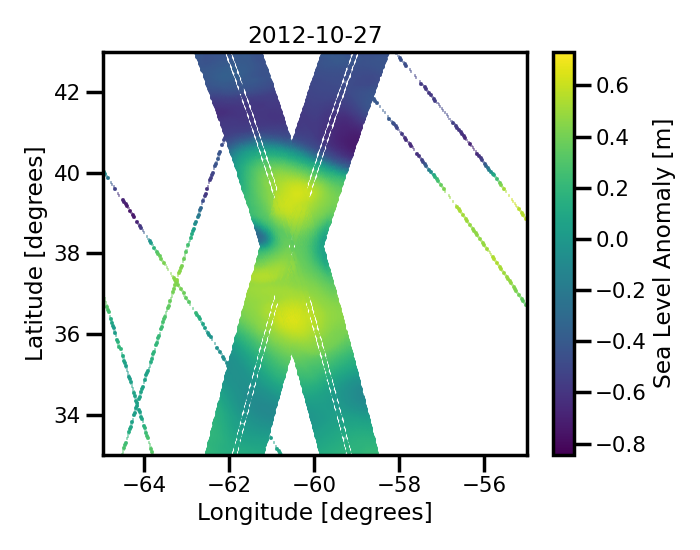
\includegraphics[width=42.5mm, height=30mm]{00_Oceanbench/content/figures/maps/sla/dc20a_ssh_anomaly_swot1nadir5_20121027.png} &
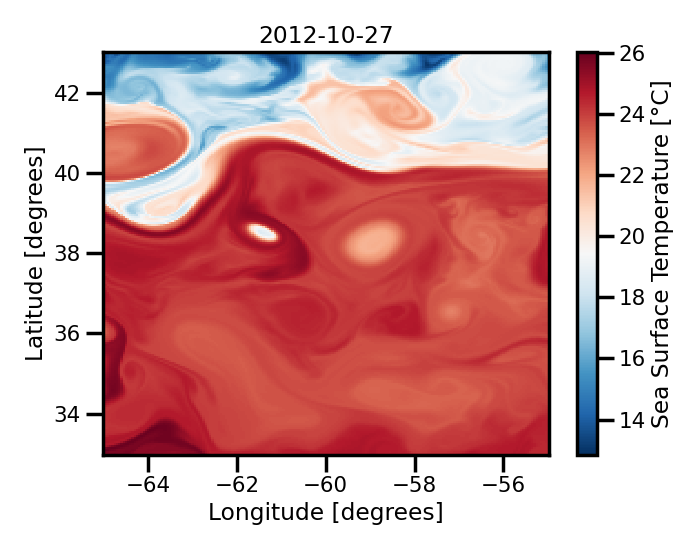
\includegraphics[width=4.25cm,height=3cm]{00_Oceanbench/content/figures/maps/sst/dc20a_nemo_sst.png}
\end{tabular}}
\makebox[\textwidth]{
\begin{tabular}{cccc}
\hspace{3mm} NEMO Simulation & 
\hspace{3mm} MIOST & 
\hspace{3mm} BFNQG & 
4DVarNet \\
\vspace{-2mm}
%%%%% SEA LEVEL ANOMALY %%%%%%%%
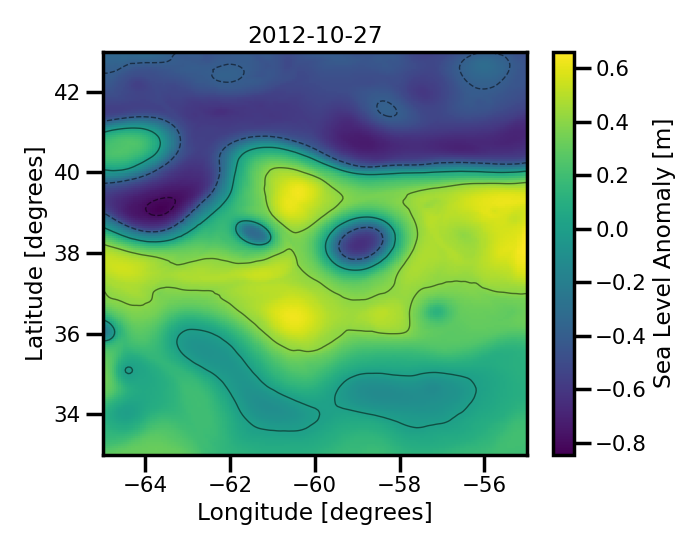
\includegraphics[trim={0 0 42mm 0},clip, width=3.20cm,height=3cm]{00_Oceanbench/content/figures/maps/sla/dc20a_nemo_sla.png} &
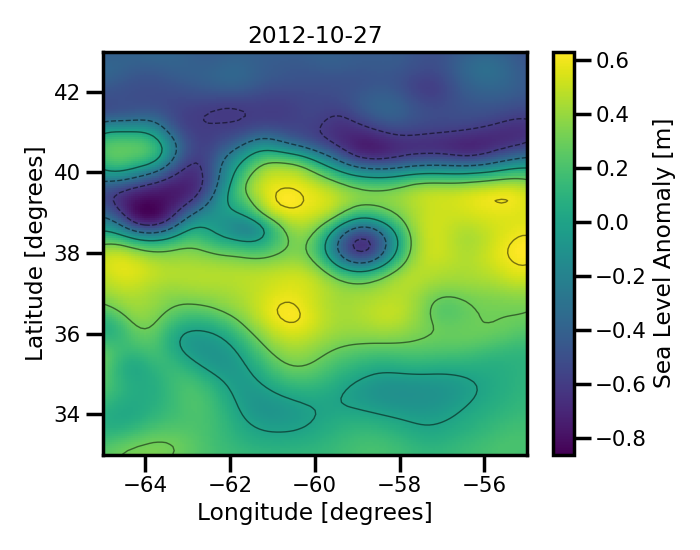
\includegraphics[trim={0 0 42mm 0},clip, width=3.2cm,height=3cm]{00_Oceanbench/content/figures/maps/sla/dc20a_miost_sla.png} &
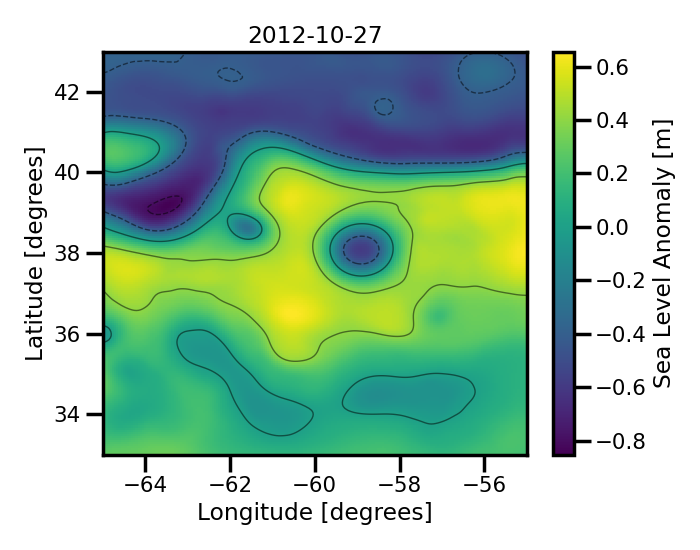
\includegraphics[trim={0 0 42mm 0},clip, width=3.2cm,height=3cm]{00_Oceanbench/content/figures/maps/sla/dc20a_bfnqg_sla.png} &
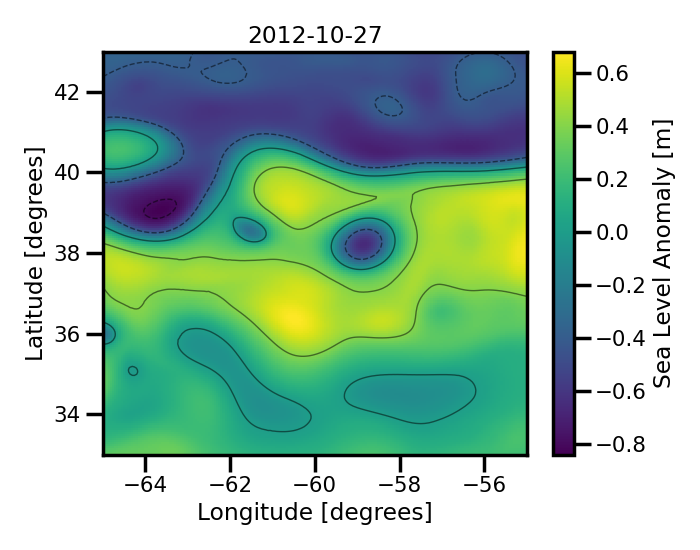
\includegraphics[width=4.0cm,height=3cm]{00_Oceanbench/content/figures/maps/sla/dc20a_4dvarnet_sla.png} \\
\vspace{-2mm}
%%%%% KINETIC ENERGY %%%%%%%%
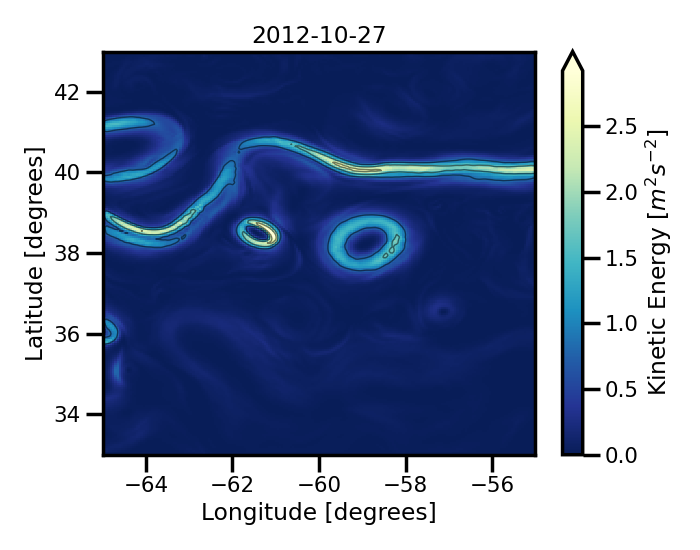
\includegraphics[trim={0 0 42mm 0},clip, width=3.20cm,height=3cm]{00_Oceanbench/content/figures/maps/ke/dc20a/nadir4/dc20a_nemo_ke.png} &
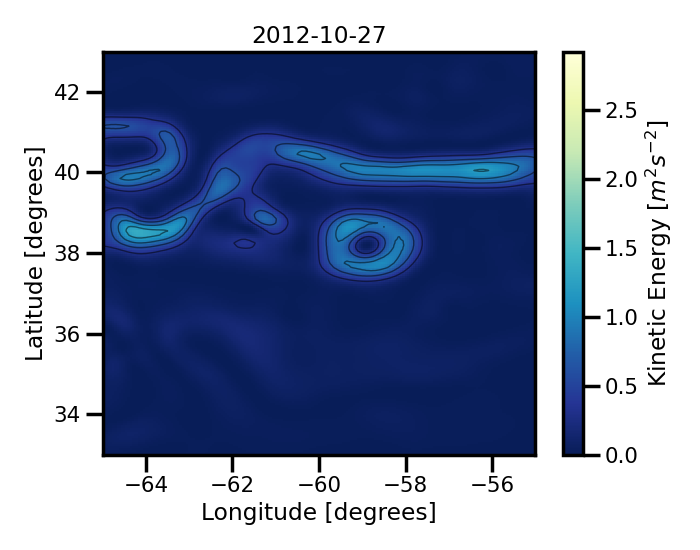
\includegraphics[trim={0 0 42mm 0},clip, width=3.2cm,height=3cm]{00_Oceanbench/content/figures/maps/ke/dc20a/nadir4/dc20a_miost_ke.png} &
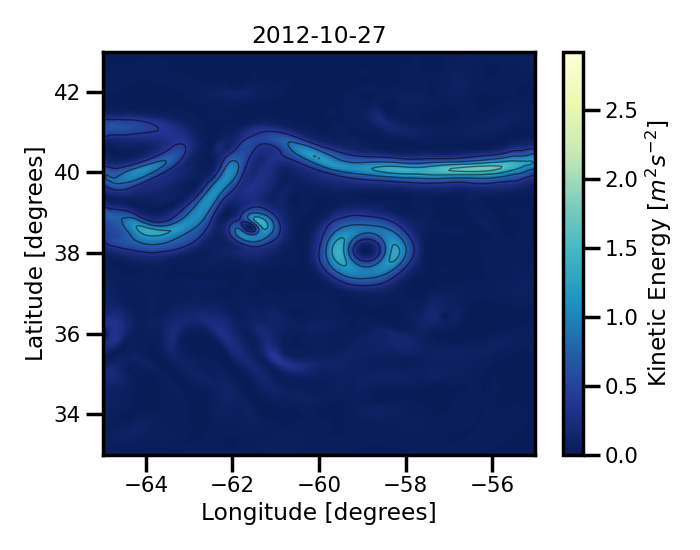
\includegraphics[trim={0 0 42mm 0},clip, width=3.2cm,height=3cm]{00_Oceanbench/content/figures/maps/ke/dc20a/nadir4/dc20a_bfnqg_ke.png} &
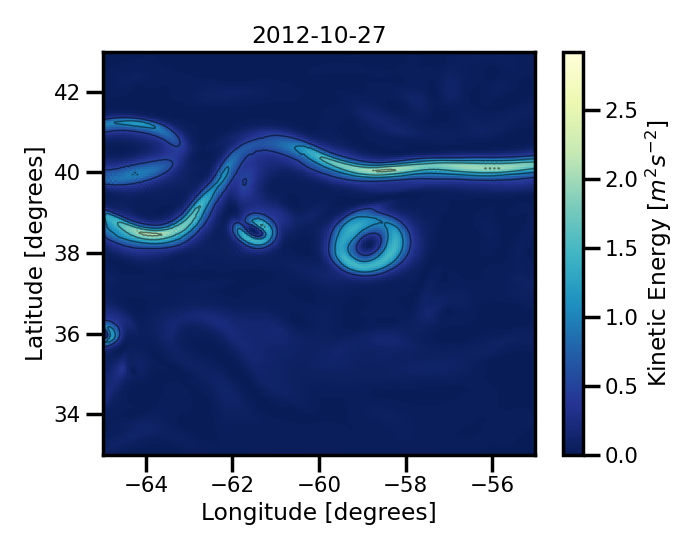
\includegraphics[width=4.0cm,height=3cm]{00_Oceanbench/content/figures/maps/ke/dc20a/nadir4/dc20a_4dvarnet_ke.png}  \\
\vspace{-2mm}
%%%%% RELATIVE VORTICITY %%%%%%%%
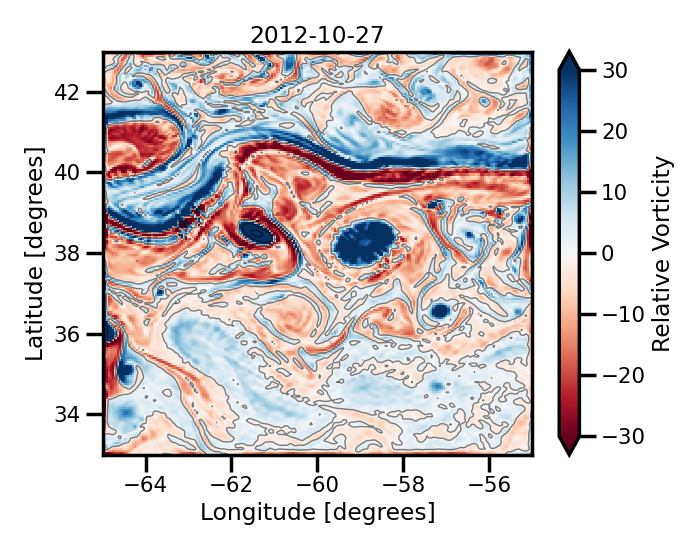
\includegraphics[trim={0 0 42mm 0},clip, width=3.20cm,height=3cm]{00_Oceanbench/content/figures/maps/rvort/dc20a/nadir4/dc20a_nemo_vort_r.png} &
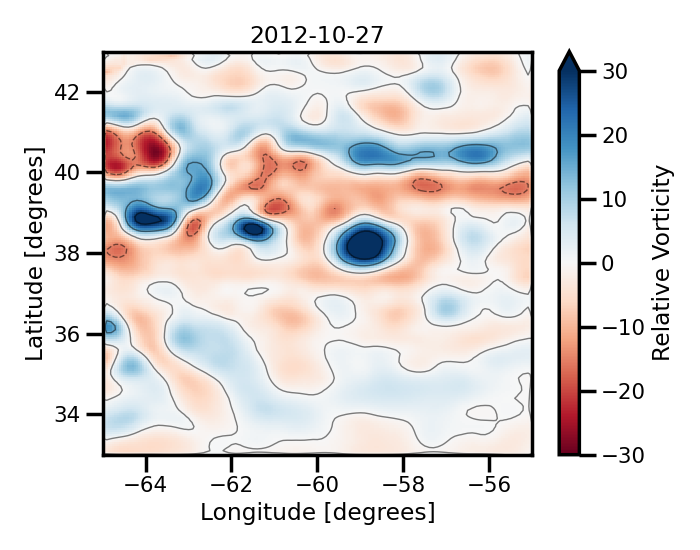
\includegraphics[trim={0 0 42mm 0},clip, width=3.2cm,height=3cm]{00_Oceanbench/content/figures/maps/rvort/dc20a/nadir4/dc20a_miost_vort_r.png} &
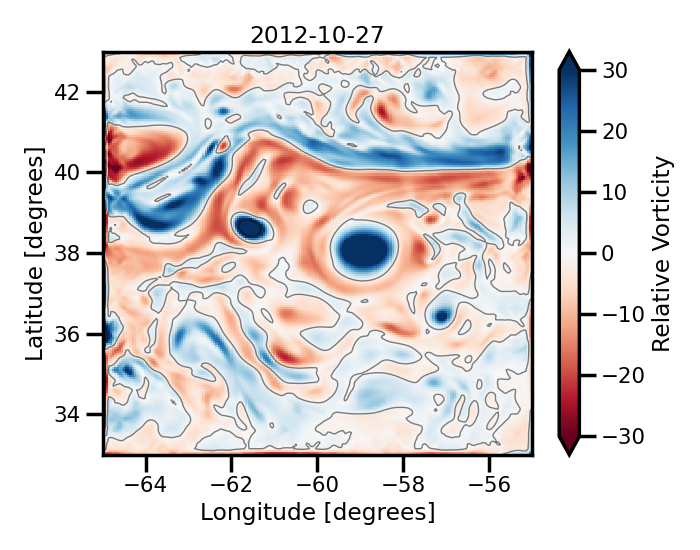
\includegraphics[trim={0 0 42mm 0},clip, width=3.2cm,height=3cm]{00_Oceanbench/content/figures/maps/rvort/dc20a/nadir4/dc20a_bfnqg_vort_r.png} &
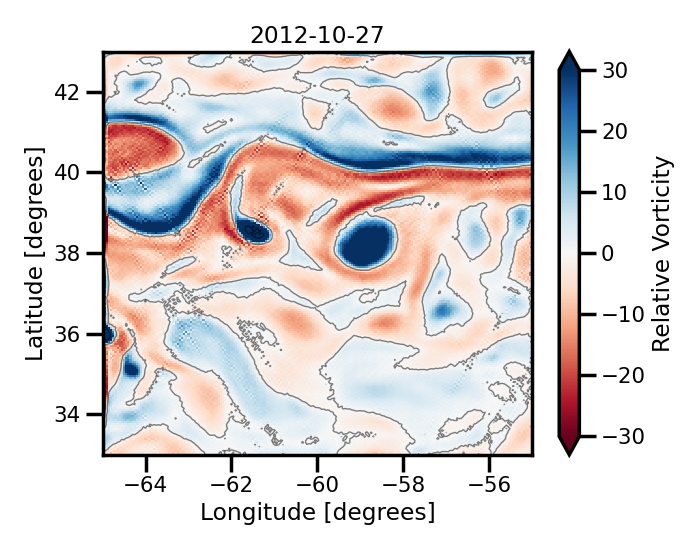
\includegraphics[width=4.0cm,height=3cm]{00_Oceanbench/content/figures/maps/rvort/dc20a/nadir4/dc20a_4dvarnet_vort_r.png}  \\
%%%%% STRAIN %%%%%%%%
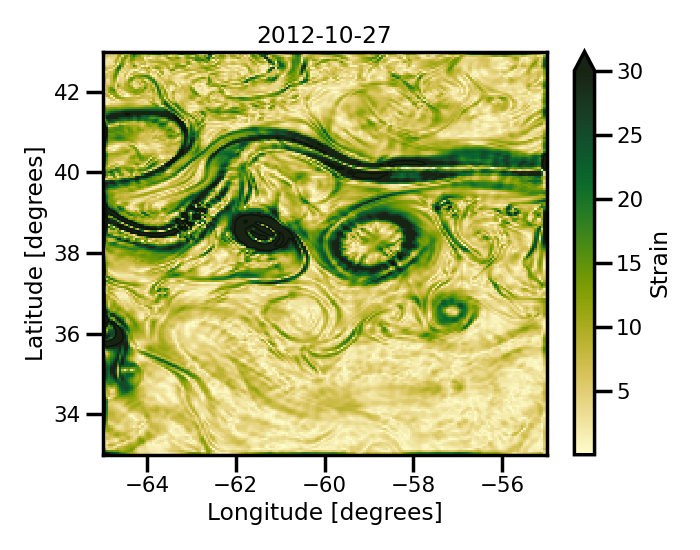
\includegraphics[trim={0 0 38mm 0},clip, width=3.20cm,height=3cm]{00_Oceanbench/content/figures/maps/strain/dc20a/nadir4/dc20a_nemo_strain.png} &
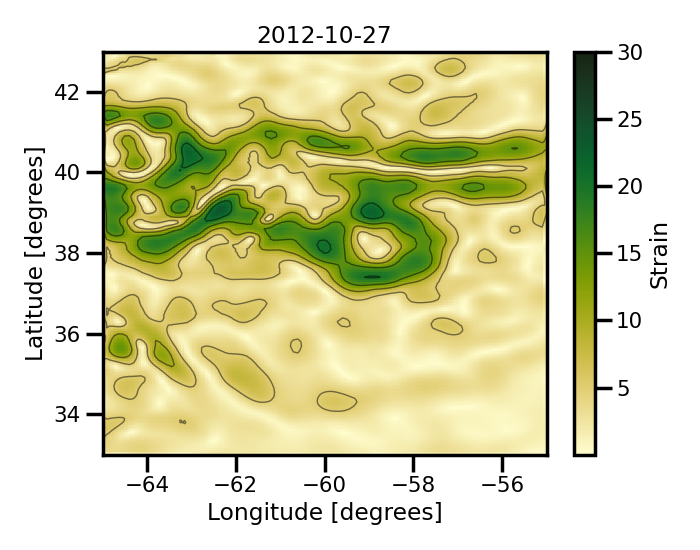
\includegraphics[trim={0 0 38mm 0},clip, width=3.2cm,height=3cm]{00_Oceanbench/content/figures/maps/strain/dc20a/nadir4/dc20a_miost_strain.png} &
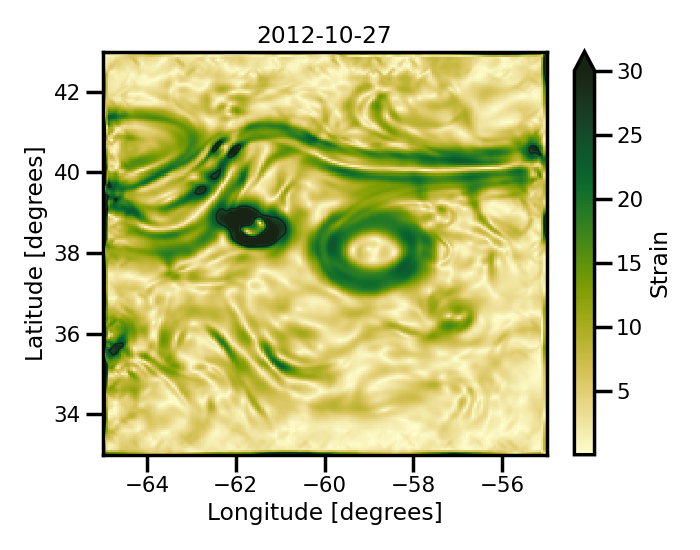
\includegraphics[trim={0 0 38mm 0},clip, width=3.2cm,height=3cm]{00_Oceanbench/content/figures/maps/strain/dc20a/nadir4/dc20a_bfnqg_strain.png} &
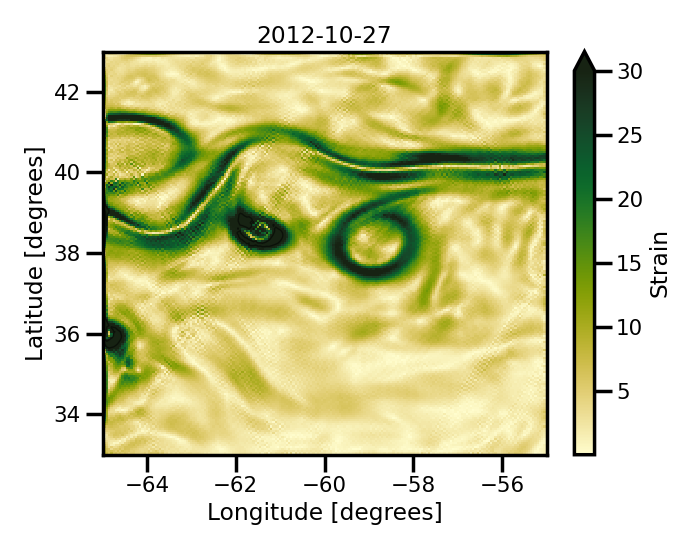
\includegraphics[width=4.0cm,height=3cm]{00_Oceanbench/content/figures/maps/strain/dc20a/nadir4/dc20a_4dvarnet_strain.png}  \\
% \vspace{-2mm}
(a) & (b) & (c) & (d)
\end{tabular}}
\vspace{-3mm}
% \caption{Row I - Isotrophic PSD. Row 2 - Isotrophic PSD Score}
\caption{
A snapshot at $27^{th}$ October, 2012 of the sea level anomaly (SLA) from the NEMO simulation for the OSSE experiment outlined in section~\ref{sec:experimental_design}. 
The top row showcases the aggregated NADIR altimetry tracks and the aggregated SWOT altimetry tracks (12 hours before and 12 hours after) as well as the SST from the NEMO simulation.
Each subsequent row showcases the following physical variables found in appendix~\ref{sec:physical_variables}: (a) Sea Level Anomaly, (b) Kinetic Energy, (c) Relative Vorticity, and (d) Strain. 
Each column in the subsequent rows showcase the following reconstructed field from the NEMO simulation found in columrn (a): (b) MIOST~\cite{MIOST}, (c) BFN-QG~\cite{BFNQG}, and (d) 4DVarNet~\cite{4DVARNETSWOT}.}
\label{fig:oceanbench_maps}
\vspace{-5mm}
\end{center}
\end{figure}


\begin{landscape}
\small
\begin{table}[ht]


\centering
\makebox[\textwidth]{
\begin{tabular}{lcclclcc}
 \toprule
     & OSSE SSH      & \multicolumn{2}{c}{OSSE SSH NADIR}                     & \multicolumn{2}{c}{OSSE SSH SWOT}                      & OSSE SST             & OSE SSH NADIR            \\ \midrule\midrule
Data Structure & Gridded              & AlongTrack           & \multicolumn{1}{c}{Gridded} & AlongTrack           & \multicolumn{1}{c}{Gridded} & Gridded              & AlongTrack           \\
     & \multicolumn{1}{l}{} & \multicolumn{1}{l}{} &                             & \multicolumn{1}{l}{} &  \\ \midrule
Source     & 
NEMO~\citep{NEMOAJAYI2020} &
NEMO~\citep{NEMOAJAYI2020} &
NEMO~\citep{NEMOAJAYI2020} &
NEMO~\citep{NEMOAJAYI2020} & 
NEMO~\citep{NEMOAJAYI2020} &
NEMO~\citep{NEMOAJAYI2020}
% \multicolumn{3}{c}{NEMO GCM\citep{NEMOAJAYI2020}}  
& Altimetry~\citep{MDSALONGTRACK} \\
Region & 
GulfStream & GulfStream & GulfStream & GulfStream &
GulfStream & GulfStream & GulfStream
\\
Domain Size [$^\circ$] &
% ($L_x\times L_y$) 
$10\times 10^\circ$ &
$10\times 10^\circ$ &
$10\times 10^\circ$ &
$10\times 10^\circ$ &
$10\times 10^\circ$ &
$10\times 10^\circ$ &
$10\times 10^\circ$ \\
Domain Size [km] &
% ($L_x\times L_y$) 
$1100\times 1100$ &
$1100\times 1100$ &
$1100\times 1100$ &
$1100\times 1100$ &
$1100\times 1100$ &
$1100\times 1100$ &
$1100\times 1100$ \\
Longitude Extent &
$[-65^\circ, -55^\circ]$ & 
$[-65^\circ, -55^\circ]$ & 
$[-65^\circ, -55^\circ]$ & 
$[-65^\circ, -55^\circ]$ & 
$[-65^\circ, -55^\circ]$ &
$[-65^\circ, -55^\circ]$ &
$[-65^\circ, -55^\circ]$ \\
Latitude Extent &
$[33^\circ, 43^\circ]$ &
$[33^\circ, 43^\circ]$ &
$[33^\circ, 43^\circ]$ &
$[33^\circ, 43^\circ]$ &
$[33^\circ, 43^\circ]$ &
$[33^\circ, 43^\circ]$ &
$[33^\circ, 43^\circ]$ \\
Resolution [$^\circ$] &
% ($\Delta_x\times \Delta_y$) 
$0.05^\circ\times 0.05^\circ$ &
N/A &
$0.05^\circ\times 0.05^\circ$ &
N/A &
$0.05^\circ\times 0.05^\circ$ &
$0.05^\circ\times 0.05^\circ$ &
N/A \\
Resolution [km] &
% ($\Delta_x\times \Delta_y$) 
$5.5\times 5.5$ &
$6$ &
$5.5\times 5.5$ &
$6$ &
$5.5\times 5.5$ &
$5.5\times 5.5$ &
$7$ \\
Grid Size &
$200\times 200$ & 
N/A &
$200\times 200$ & 
N/A &
$200\times 200$ & 
$200\times 200$ & 
N/A \\
Num. Datapoints &
$\sim$14.6M & 
$\sim$205K & 
$\sim$14.6M & 
$\sim$955K & 
$\sim$14.6M & 
$\sim$14.6M & 
$\sim$1.79M \\ \midrule
Period Start & 
2012-10-01 & 2012-10-01 & 2012-10-01 & 2012-10-01 & 
2012-10-01 & 2012-10-01 & 2016-12-01 \\
Period End & 
2013-09-30 & 2013-09-30 & 2013-09-30 & 2013-09-30 & 
2013-09-30 & 2013-09-30 & 2018-01-31 \\
Frequency  & 
Daily & 1 Hz  & Daily & 1 Hz  & Daily & Daily & 1 Hz \\ 
Period Length & 365 Days & 365 Days & 365 Days &
365 Days & 365 Days & 365 Days & 427 Days \\
\midrule
Evaluation Start & 
2012-10-22 & 2012-10-22 & 2012-10-22 & 2012-10-22 & 
2012-10-22 & 2012-10-22 & 2017-01-01 \\
Evaluation End & 
2012-12-02 & 2012-12-02 & 2012-12-02 & 2012-12-02 & 
2012-12-02 & 2012-12-02 & 2017-12-31 \\ 
Evaluation Length & 45 Days & 45 Days & 45 Days &
45 Days & 45 Days & 45 Days & 365 Days \\
\bottomrule
\end{tabular}}
\caption{This table gives an extended overview of the datasets provided to complete the data challenges listed in~\ref{sec:data_challenges} and~\ref{sec:data_challenges_extended}. The OSSE SST and SSH are outputs from come from the free run NEMO model~\citep{NEMOAJAYI2020}. The OSSE NADIR and SWOT are pseudo-observations generated from the NEMO simulation. We provide the original simulated satellite tracks as well as a gridded version at the same resolution as the simulation. 
}
\label{c5tb:datasetsmega}
\end{table}
\end{landscape}

% \subsubsection{Observing System Experiments (OSE)} \label{sec:ose}

\textbf{Observing System Experiments (OSE)}. As more observations have become available over the past few decades, we can also design experiments using real data. 
This involves aggregating as many observations from real ocean altimetry satellites as possible with some specific independent subset left out for evaluation purposes.
A major downside to OSE experiments is that the sparsity and spatial coverage of the observations narrow the possible scope of performance metrics and make it very challenging to learn directly from observation datasets. 
The current standard altimetry data are high resolution but cover a tiny area. 
As such, it can only inform fine-scale SSH patterns in the along-track satellite direction and cannot explicitly reveal two-dimensional patterns. 
Despite these drawbacks, it provides a quantitative evaluation of the generalizability of the ML methods concerning the true ocean state.




%and so it fails to capture many of the dynamical regimes we are interested in, i.e. mesoscale and sub-mesoscale processes. 
%However, it is still advantageous (and preferable) to include these experiments because these reflect the true ocean state and will help with the generalizability of the ML methods.

\begin{figure}[H]
\small
\begin{center}
\setlength{\tabcolsep}{2pt}
\makebox[\textwidth]{
\begin{tabular}{ccc}
% $\mathcal X$ & $\hat \z = \bG_\theta(\x)$ & $\x = \bG_\theta^{-1} (\hat \z)$\\[0mm]
% NATL60&
% \multicolumn{2}{c}{\includegraphics[width=6.25cm,height=4.5cm]{content/figures/exp_natl60/psd_st/osse_2020a_psd_natl60}} 
% \\
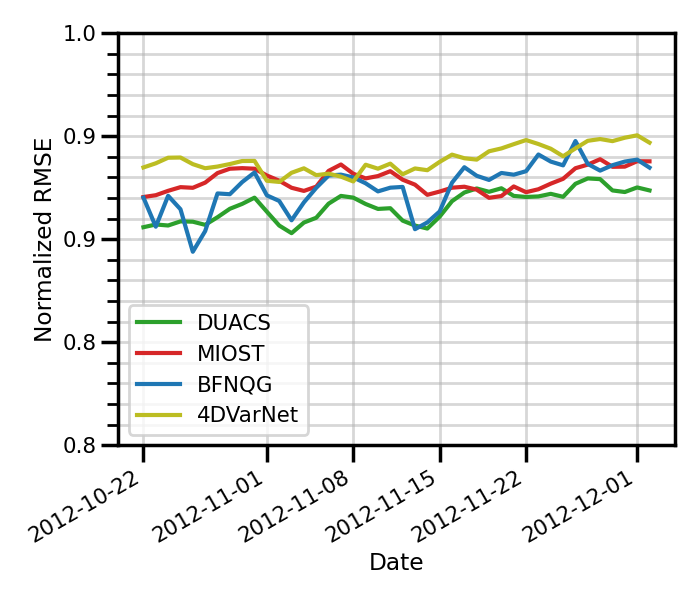
\includegraphics[width=3.75cm,height=3.25cm]{00_Oceanbench/content/figures/stats/nrmse_space.png} &
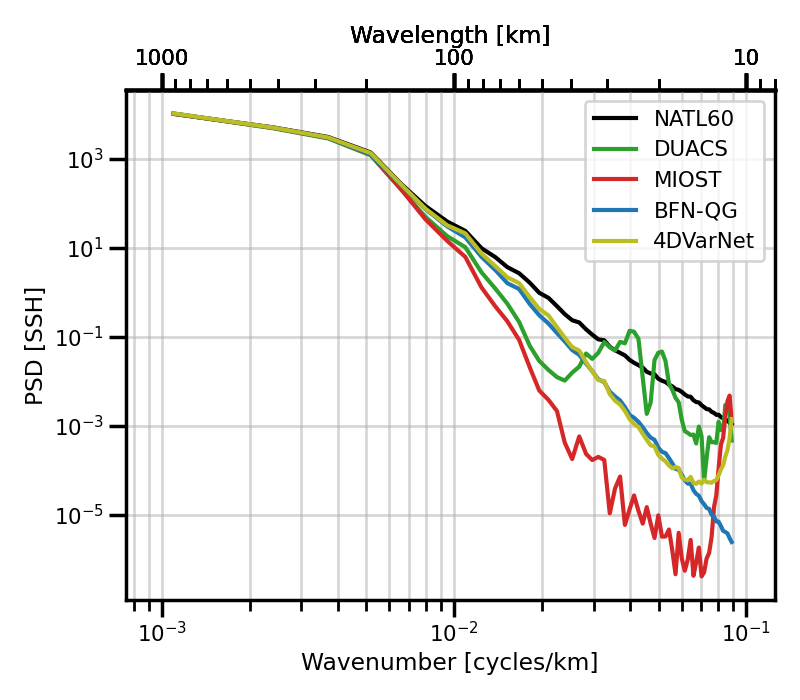
\includegraphics[width=4.25cm,height=3.5cm]{00_Oceanbench/content/figures/psd_isotropic/dc20a/nadir4/dc20a_psd_iso_ssh.png} &
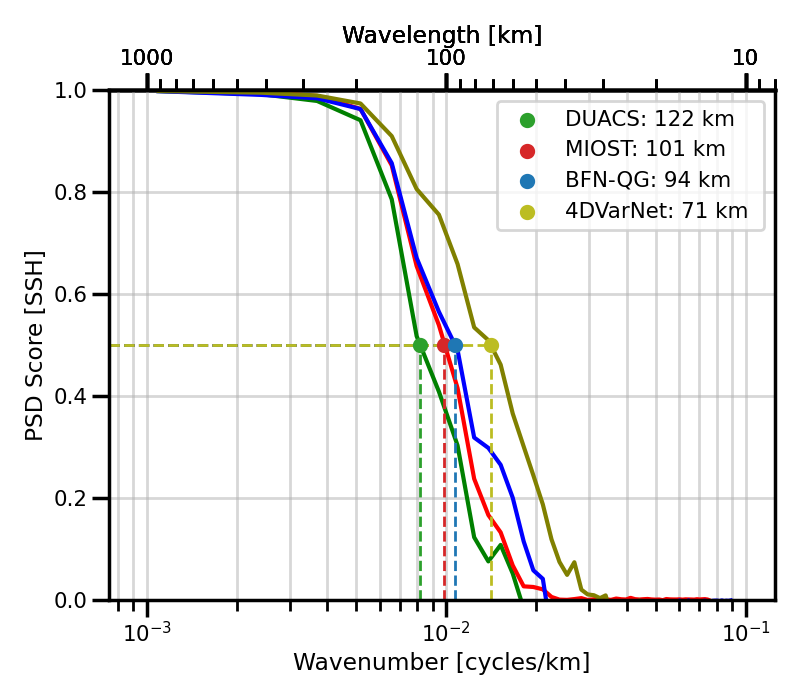
\includegraphics[width=4.25cm,height=3.5cm]{00_Oceanbench/content/figures/psd_isotropic/dc20a/nadir4/dc20a_psd_score_iso_ssh.png} 
\\
(a) Normalized RMSE &
(b) Isotropic Power Spectrum &
(c) Isotropic Power Spectrum Score
\end{tabular}}
\makebox[\textwidth]{
\begin{tabular}{cccc}
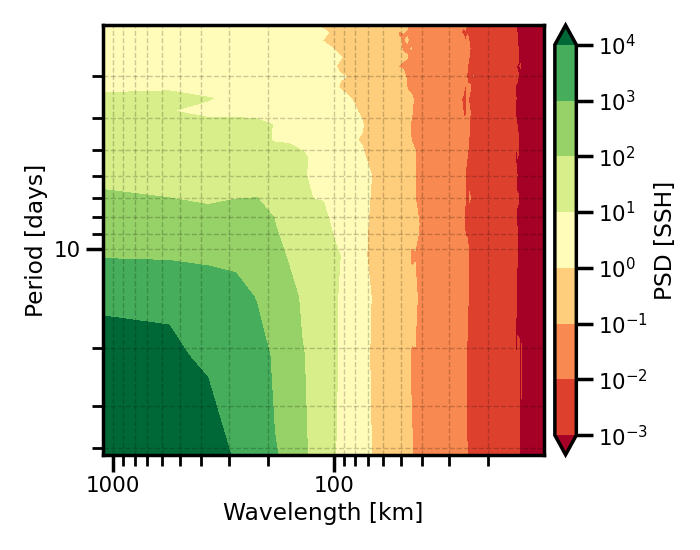
\includegraphics[trim={0 0 0mm 0},clip, width=4.20cm,height=3cm]{00_Oceanbench/content/figures/psd_spacetime/dc20a/nadir4/dc20a_psd_spacetime_nemo_nadir4_ssh.png}  &
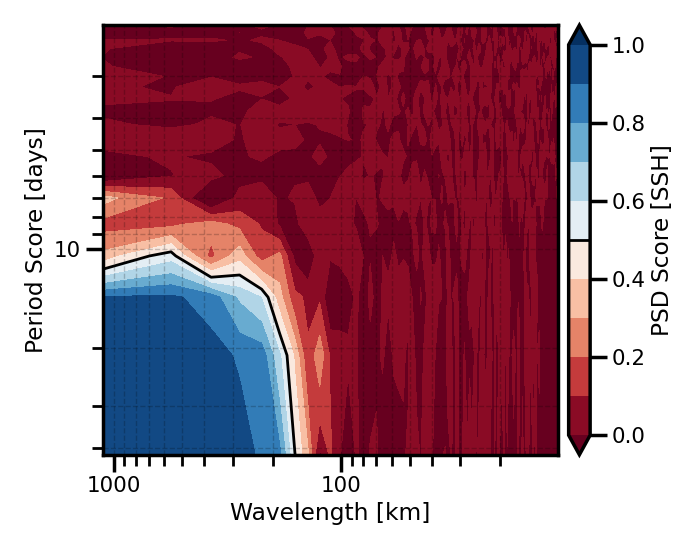
\includegraphics[trim={20mm 0 34mm 0},clip, width=2.9cm,height=3cm]{00_Oceanbench/content/figures/psd_spacetime/dc20a/nadir4/dc20a_psd_spacetime_score_miost_nadir4_ssh.png} &
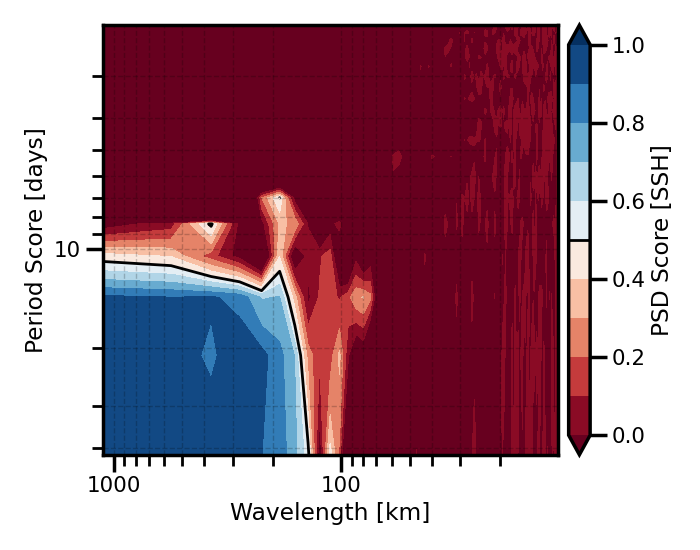
\includegraphics[trim={20mm 0 34mm 0},clip, width=2.9cm,height=3cm]{00_Oceanbench/content/figures/psd_spacetime/dc20a/nadir4/dc20a_psd_spacetime_score_bfnqg_nadir4_ssh.png} &
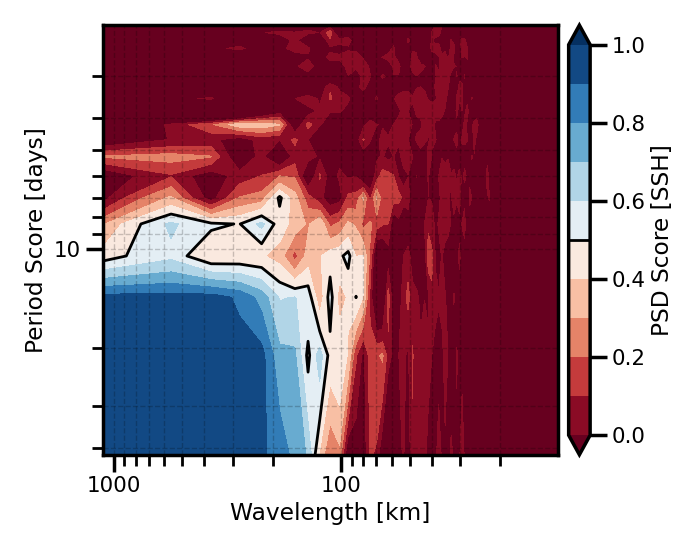
\includegraphics[trim={20mm 0 0 0},clip, width=3.5cm,height=3cm]{00_Oceanbench/content/figures/psd_spacetime/dc20a/nadir4/dc20a_psd_spacetime_score_4dvarnet_nadir4_ssh.png} \\
(d) NEMO Simulation &
(e) MIOST &
(f) BFN-QG &
(g) 4DVarNet
\end{tabular}}
% % \vspace{-4mm}
% \caption{Row I - Isotrophic PSD. Row 2 - Isotrophic PSD Score}
\caption{This figure showcases some statistics for evaluation of the SSH field reconstructions for the OSSE NADIR experiment outlined in section~\ref{sec:interp_challenge}. Subfigure (a) showcases the normalized root mean squared error (nRMSE), (b) showcases the isotropic power spectrum decomposition (PSD), (c) showcases isotropic PSD scores.
The bottom row showcases the space-time PSD for the NEMO simulation (subfigure (d)) and the PSD scores for three reconstruction models: (e) the MIOST model~\cite{MIOST}, (f) the BFN-QG model~\cite{BFNQG}, and (g) the 4DVarNet model~\cite{4DVARNETSWOT}.
}
% \vspace{-5mm}
\label{fig:oceanbench_psd}
\end{center}
\end{figure}


%
\subsection*{Data Challenges} \label{sec:data_challenges}
We rely on existing OSSE and OSE experiments for SSH interpolation designed by domain experts~\cite{DCOSEGULFSSH,DCOSSEGULFSSH} and recast them into \texttt{OceanBench} framework to deliver a ML-ready benchmarking suites. 
The selected data challenges for this first edition address SSH interpolation for a 1000km$\times$1000km Gulfstream region. We describe each of them below.

% \subsection*{OSSE NADIR} \label{sec:osse_nadir}
\textbf{Experiment I (\textit{OSSE NADIR})} addresses SSH interpolation using NADIR altimetry tracks which are very fine, thin ocean satellite observations (see Figure~\ref{fig:oceanbench_maps}). It relies on an OSSE using high-resolution ($1/60^\circ$ resolution) ocean simulations generated by the NEMO model over one year with a whole field every day. 
The reference simulation is the \textit{NATL60} simulation based on the NEMO model~\cite{NEMOAJAYI2020}. 
This particular simulation was run over an entire year without any tidal forcing.
The simulation provides the outputs of SSH, SST, sea surface salinity (SSS) and the u,v velocities every 1 hour.
For the purposes of this data challenge, the spatial domain is over the Gulfstream with a spatial domain of $[-65^\circ, -55^\circ]$ longitude and $[33^\circ, 43^\circ]$ latitude.
The resolution of the original simulation is 1/60$^\circ$ resolution with hourly snapshots, and we consider a daily downsampled trajectory at 1/20$^\circ$ for the data challenge which results in a 365x200x200 spatio-temporal grid.
This simulation resolves finescale dynamical processes ($\sim$15km) which makes it a good test bed for creating an OSSE environment for mapping.
The SSH observations include simulations of ocean satellite NADIR tracks.
In particular, they are simulations of Topex-Poseidon, Jason 1, Geosat Follow-On, and Envisat.
There is no observation error considered within the challenge.
We use a the entire period from 2012-10-10 until 2013-09-30.
A training period is only from 2013-01-02 to 2013-09-30 where the users can use the reference simulation as well as all available simulated observations.
The evaluation period is from 2012-10-22 to 2012-12-02 (i.e. 41 days) which is considered decorrelated from the training period. 
During the evaluation period, the user cannot use the reference NATL60 simulation but they can use all available simulated observations. There is also a spin-up period allowance from 2012-10-01 where the user can also use all available simulated observations.

% \subsection*{OSSE SWOT \& OSSE SST} \label{sec:osse_swot_sst}
\textbf{Experiment II (\textit{OSSE SWOT})} addresses SSH interpolation using jointly NADIR and SWOT altimetry data where we complement the \textbf{OSSE NADIR} configuration with simulated SWOT observations.
SWOT is a new satellite altimetry mission with a much higher spatial coverage but a much lower temporal resolution as illustrated in Figure~\ref{fig:oceanbench_maps}.
The higher spatial resolution allows us to see structures at a smaller resolution but at the cost of a massive influx of observations (over $\times$100).

\textbf{Experiment III (\textit{OSSE SST})} addresses SSH interpolation using altimetry and SST satellite data jointly. We complement the \textbf{OSSE SWOT} challenge with simulated SST observations. 
Satellite-derived SST observations are more abundantly available in natural operational settings than SSH at a finer resolution, and structures have visible similarities~\cite{SWOT,BFNQG}.
So this challenge allows for methods to take advantage of multi-modal learning~\cite{4DVARNETSST,SSHInterpAttention}.

For the OSSE SWOT and OSSE SST experiments, the reference simulation, domain, and evaluation period is the same as the OSSE NADIR experiment.
However, the OSSE SWOT includes simulated observations of the novel KaRIN sensor recently deployed during the SWOT mission, the pseudo-observations were generated using the SWOT simulator~\cite{SWOT}. 
This OSSE SST experiment allows the users to utilize the full fields of SST as inputs to help reconstruct the SSH field in conjunction with the NADIR and SWOT SSH observation.
Because the SST comes from the same NATL60 simulation, the geometry characteristics SST and SSH are exactly the same.

% \subsection*{OSE NADIR} \label{sec:ose_nadir}

\textbf{Experiment IV (\textit{OSE NADIR})} addresses SSH interpolation for real NADIR altimetry data. 
In contrast to the three OSSE data challenges, it only looks at actual observations aggregated from the currently available ocean altimetry data from actual satellites. 
It involves a similar space-time sampling as Experiment (\textbf{OSSE NADIR}) to evaluate the generalization of ML methods trained in Experiment I to real altimetry data. 
The training problem's complexity increases significantly due to the reference dataset's sparsity compared with the \textbf{OSSE NADIR} dataset. 
One may also explore transfer learning or fine-tuning strategies from the available OSSE dataset. 

The OSE NADIR experiment only uses real observations aggregated from different altimeters. These SSH observations include observations from the SARAL/Altika, Jason 2, Jason 3, Sentinel 3A, Haiyang-2A and Cryosat-2 altimeters. The Cryosat-2 altimeter is used as the independent evaluation track used to assess the performance of the reconstructed SSH field.
\newpage


\subsection*{Metrics} \label{sec:metrics}

There are many metrics that are standard within the ML community but unconvincing for many parts the geoscience community. 
Specifically, many of these standard scores do not capture the important optimization criteria in the scientific machine learning tasks.
However, there is not consensus within domain-specific communities about the perfect metric which captures every aspect we are interested.
Therefore, we should have a variety of scores from different perspectives to really assess the pros and cons of each method we wish to evaluate thoroughly. 
Below, we outline two sets of scores we use within this framework: skill scores and spectral scores.

\textbf{Skill Scores}

We classify one set of metrics as \textit{skill scores}. 
These are globally averaged metrics which tend to operate within the real space.
Some examples include the root mean squared error (RMSE), the normalized root mean squared (nRMSE) error, and the nRMSE score.
The RMSE metric can also be calculated w.r.t. the spatial domain, temporal domain or both. 
For example, figure~\ref{fig:oceanbench_psd} showcases the nRMSE score calculated only on the spatial domain and visualized for each time step.
%
\begin{align}
    \text{RMSE}: &&\text{RMSE}(\eta,\hat{\eta}) &= ||\eta - \hat{\eta}||_2 \label{eq:RMSE}\\
    % \text{RMSE}_t: &&\text{RMSE}_t(\eta,\hat{\eta}; t) &= ||\eta(t) - \hat{\eta}(t)||_2 \label{eq:RMSE_t}\\
    \text{nRMSE}: &&\text{nRMSE}(\eta,\hat{\eta}) &= \frac{\text{RMSE}(\eta,\hat{\eta})}{||\eta||_2} \label{eq:nRMSE} \\
    \text{nRMSE}_{\text{score}}: &&\text{nRMSE}_{\text{score}}(\eta,\hat{\eta}) &= 1 - \text{nRMSE}(\eta,\hat{\eta})
    \label{eq:nRMSE_score}
\end{align}
%
However, we are not limited to just the standard MSE metrics.
We can easily incorporate more higher-order statistics like the Centered Kernel Alignment (CKA)~\cite{METRICSCKA} or information theory metrics like mutual information (MI)~\cite{METRICSITRBIG,METRICSITRBIG2}.
In addition, we could also utilize the same metrics in the frequency domain as is done in~\citep{PDEBench}.

\textbf{Spectral Scores}

Another class of scores that we use in \texttt{OceanBench} are the \textit{spectral scores}. These scores are calculated within the spectral space via the wavenumber power spectral density (PSD). 
This provides a spatial-scale-dependent metric which is useful for identifying the largest and smallest scales that were resolved by the reconstruction map. 
In general, we use these to measure the expected energy at different spatiotemporal scales and we can also construct custom score functions which gives us a summary statistic for how well we reconstructed certain scales.
%
\begin{align}
    \text{PSD}: &&\text{PSD}(\eta) &= \sum_{k_{min}}^{k_{max}}\|\mathcal{\mathcal{F}(\eta)}\|^2\label{psd}\\
    \text{PSD}_{score}: &&\text{PSD}_{score}(\eta,\hat{\eta}) &= 1 - \frac{\text{PSD}(\eta - \hat{\eta})}{\text{PSD}(\eta)} \label{eq:psd_score}
\end{align}
%
where $\mathcal{F}$ is the Fast Fourier Transformation (FFT). 
In our application, there are various ways to construct the PSD which depend on the FFT transformation.
We denote the \textit{space-time PSD} as $\lambda_\mathbf{x}$ which does the 2D FFT in the longitude and time direction, then takes the average over the latitude.
We denote the \textit{space-time PSD} as $\lambda_\mathbf{t}$ which does the 2D FFT in the longitude and latitude direction, then takes the average over the time.
We denote the \textit{isotropic PSD} as $\lambda_r$ which assumes a radial relationship in the spatial domain and then averages over the temporal domain.
Lastly, we denote the standard PSD score as $\lambda_a$ which is the 1D FFT over a prescribed distance along the satellite track; this is what is done for the OSE NADIR experiment.
We recognize that the FFT configurations are limited due to their global treatment of the spectral domain and we need more specialized metrics to handle the local scales.
This opens the door to new metrics that handle such cases such as the Wavelet transformation~\cite{METRICSWAVELET}.

\begin{figure}[t!]
\small
\begin{center}
\setlength{\tabcolsep}{1pt}
\begin{tabular}{cccc}
\hspace{3mm} Task OSSE & 
 Task OSSE & 
\hspace{-10mm} Task OSSE & 
\hspace{-10mm}Task OSE \\
\hspace{3mm}  Nadir & 
 Nadir + SWOT & 
\hspace{-10mm} Nadir + SST & 
\hspace{-10mm}Nadir \\
%\vspace{-2mm}
%%%%% SSH %%%%%%%%
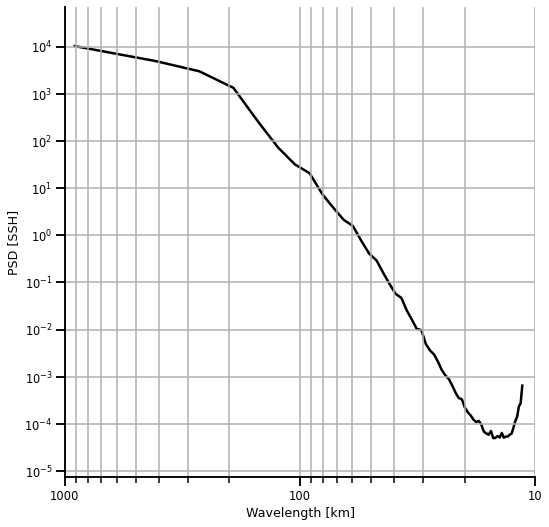
\includegraphics[trim={0 0 0 0},clip, width=3.70cm,height=3.5cm]{00_Oceanbench/content/figures/fourdvarnet_figs/osse_gf_nadir_isotrop.png} &
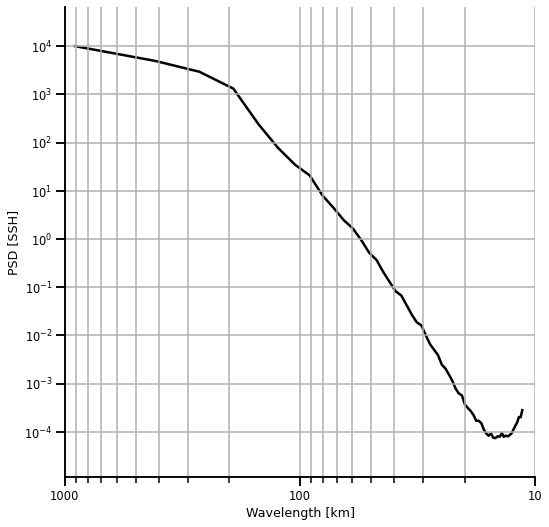
\includegraphics[trim={18mm 0 0 0},clip, width=3.3cm,height=3.5cm]{00_Oceanbench/content/figures/fourdvarnet_figs/osse_gf_nadirswot_isotrop.png} &
\hspace{-5mm}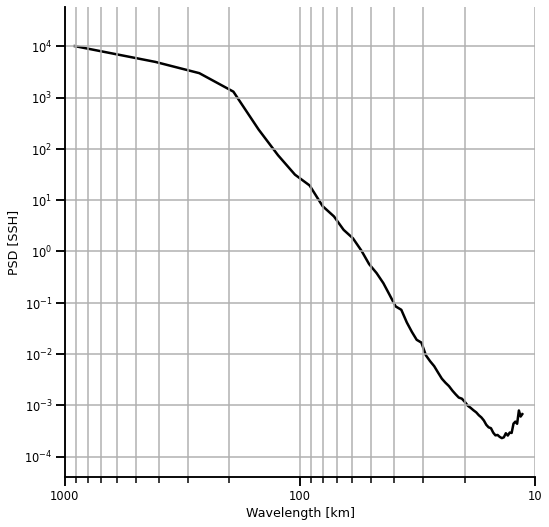
\includegraphics[trim={18mm 0 0 0},clip, width=3.3cm,height=3.5cm]{00_Oceanbench/content/figures/fourdvarnet_figs/osse_gf_nadir_sst_isotrop.png} &
\hspace{-10mm}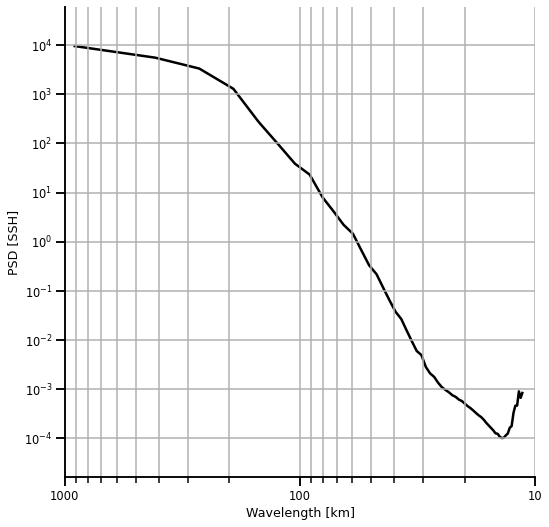
\includegraphics[trim={18mm 0 0 0},clip,width=3.3cm,height=3.5cm]{00_Oceanbench/content/figures/fourdvarnet_figs/ose_gf_isotrop.png} \\
%\vspace{3mm}
%%%%% KINETIC ENERGY %%%%%%%%
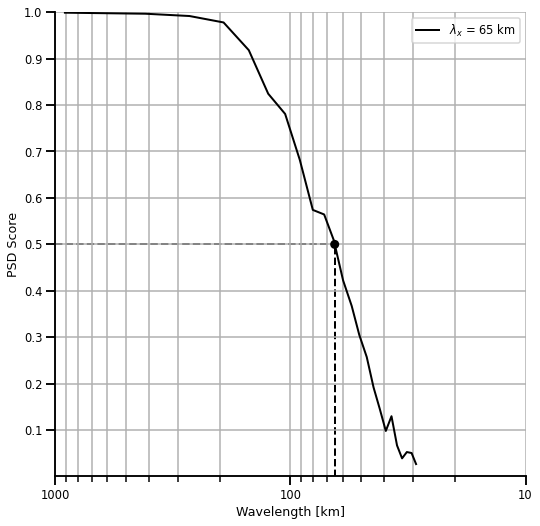
\includegraphics[trim={0 0 0 0}, clip, width=3.70cm,height=3.5cm]{00_Oceanbench/content/figures/fourdvarnet_figs/osse_gf_nadir_1d_psd_score.png} &
\hspace{1mm}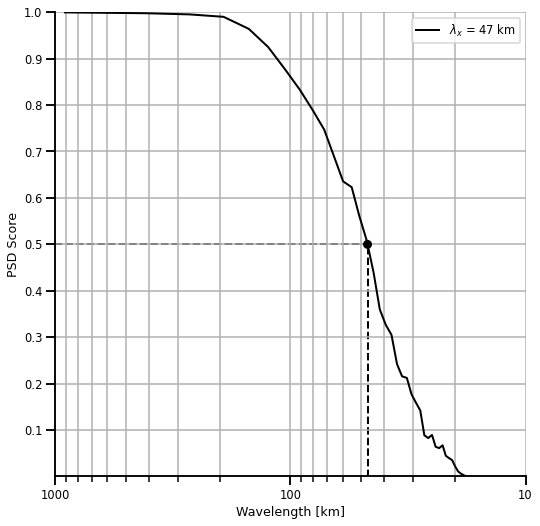
\includegraphics[trim={18mm 0 0 0},clip, width=3.3cm,height=3.5cm]{00_Oceanbench/content/figures/fourdvarnet_figs/osse_gf_nadirswot_1d_psd_score.png} &
\hspace{-4mm}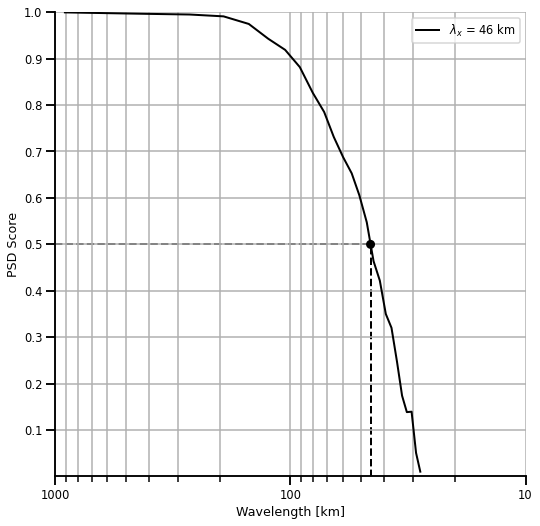
\includegraphics[trim={18mm 0 0 0},clip, width=3.3cm,height=3.5cm]{00_Oceanbench/content/figures/fourdvarnet_figs/osse_gf_nadir_sst_1d_psd_score.png} &
\hspace{-10mm}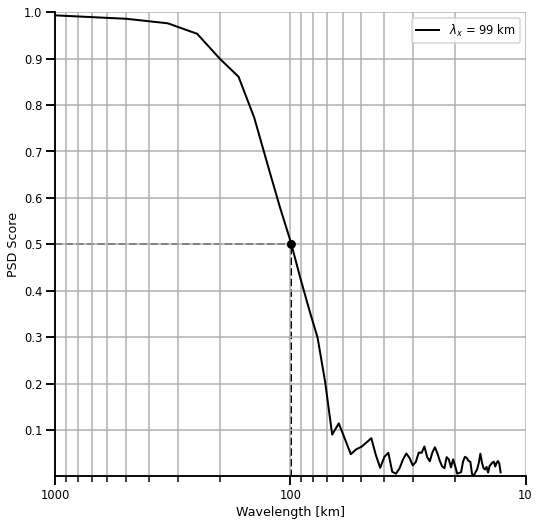
\includegraphics[trim={18mm 0 0 0},clip,width=3.3cm,height=3.5cm]{00_Oceanbench/content/figures/fourdvarnet_figs/ose_gf_1d_psd_score.png} \\
%%%%% RELATIVE VORTICITY %%%%%%%%
\hspace{-4mm}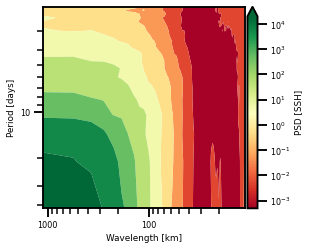
\includegraphics[trim={0 0 23mm 0},clip, width=3.65cm,height=3.5cm]{00_Oceanbench/content/figures/fourdvarnet_figs/osse_gf_nadir_psd_spacetime.png} &
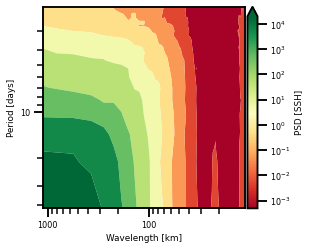
\includegraphics[trim={14mm 0 23mm 0},clip, width=3cm,height=3.5cm]{00_Oceanbench/content/figures/fourdvarnet_figs/osse_gf_nadirswot_psd_spacetime.png} &
\hspace{-5mm}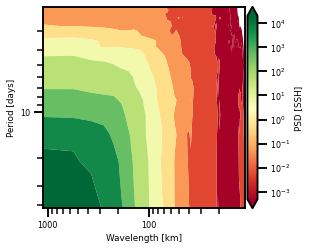
\includegraphics[trim={14mm 0 23mm 0},clip, width=3cm,height=3.5cm]{00_Oceanbench/content/figures/fourdvarnet_figs/osse_gf_nadir_sst_psd_spacetime.png} &
\hspace{-5mm}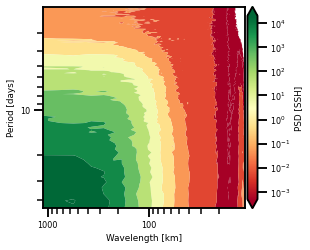
\includegraphics[trim={14mm 0 0 0},clip,width=3.8cm,height=3.5cm]{00_Oceanbench/content/figures/fourdvarnet_figs/ose_gf_psd_spacetime.png} \\
%%%%% STRAIN %%%%%%%%
\hspace{-4mm}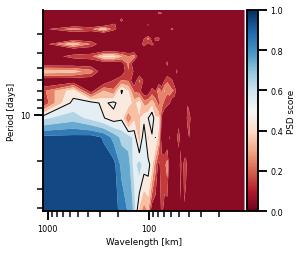
\includegraphics[trim={0 0 23mm 0},clip, width=3.70cm,height=3.5cm]{00_Oceanbench/content/figures/fourdvarnet_figs/osse_gf_nadir_psd_spacetime_score.png} &
\hspace{-2mm}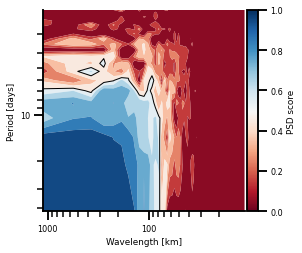
\includegraphics[trim={13mm 0 23mm 0},clip, width=3.1cm,height=3.5cm]{00_Oceanbench/content/figures/fourdvarnet_figs/osse_gf_nadirswot_psd_spacetime_score.png} &
\hspace{1mm}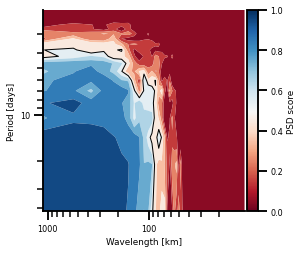
\includegraphics[trim={13mm 0 0 0},clip, width=3.8cm,height=3.5cm]{00_Oceanbench/content/figures/fourdvarnet_figs/osse_gf_nadir_sst_psd_spacetime_score.png} &
 \\
% \vspace{-2mm}
 \hspace{1mm} (a) & \hspace{-5mm} (b) & \hspace{-8mm}(c) & \hspace{-10mm}(d)
\end{tabular}
\vspace{-3mm}
% \caption{Row I - Isotrophic PSD. Row 2 - Isotrophic PSD Score}
\caption{
Power spectrum and associated scores of the 4dVarNet method for each of the four tasks.
The row display in order: (1) the isotropic PSD, (2) the spatial PSD score (using the isotropic PSD for the first three rows and along track PSD for the last row), (3) the space-time PSD, (4) The spacetime PSD score available only in OSSE task.  }

\vspace{-5mm}
\label{fig:oceanbench_psd_4dvarnet}
\end{center}
\end{figure}


\subsection*{Physical Variables} \label{sec:physical_variables}

We have access to many physical quantities which can be derived from sea surface height. 
This gives us a way to analyze how effective and trustworthy are our reconstructions. 
Many machine learning methods are unconstrained so they may provide solutions that are physically inconsistent and visualizing the field is a very easy eye test to assess the validity. 
In addition to post analysis, one could include some of these derived quantities maybe useful as additional inputs to the system and/or constraints to the loss function. 
Recall the spatiotemporal coordinates from equation~\ref{eq:spatiotemporal_coords}, 
we use the same coordinates for the subsequent physical quantities. \textbf{Sea Surface Height} is the deviation of the height of the ocean surface from the geoid of the Earth. We can define it as:
\begin{align}
	\text{Sea Surface Height }[m]:&& \quad
 \eta &= \boldsymbol{\eta}(\mathbf{x},t)&& \quad \Omega\times \mathcal{T}\rightarrow\mathbb{R} \label{eq:ssh}
\end{align}
This quantity is the actual value that is given from the satellite altimeters and is presented in the products for SSH maps~\cite{DUACS}. An example can be seen in the first row of figure~\ref{fig:oceanbench_maps_4dvarnet}.

\textbf{Sea Surface Anomaly} is the anomaly wrt to the spatial mean which is defined by
\begin{align}
	\text{Sea Level Anomaly }[m]:&& \quad
 \bar{\eta} &= \boldsymbol{\eta}(\mathbf{x},t) - \bar{\eta}(t) &&
 \quad \Omega\times \mathcal{T}\rightarrow\mathbb{R} \label{eq:sla}
\end{align}
where $\bar{\eta}(t)$ is the spatial average of the field at each time step.  
An example can be seen in the first row of figure~\ref{fig:oceanbench_maps}.

Another important quantity is the \textbf{geostrophic velocities} in the zonal and meridional directions. This is given by
\begin{align}
	\text{Zonal Velocity}[ms^{-2}]:&& \quad
 u &= -\frac{g}{f_0}\frac{\partial \eta}{\partial y} &&
 \quad \Omega\times \mathcal{T}\rightarrow\mathbb{R} \label{eq:u_vel} \\
	\text{Meridional Velocity}[ms^{-2}]:&& \quad
 v &= \frac{g}{f_0}\frac{\partial \eta}{\partial x} &&
 \quad \Omega\times \mathcal{T}\rightarrow\mathbb{R} \label{eq:v_vel}
\end{align}
where $g$ is the gravitational constant and $f_0$ is the mean Coriolis parameter. These quantities are important as they can be an related to the sea surface current. The geostrophic assumption is a very strong assumption however it can still be an important indicator variable. The \textbf{kinetic energy} is a way to summarize the (geostrophic) velocities as the total energy of the system. This is given by
\begin{equation} \label{eq:kineticenergy}
    KE = \frac{1}{2}\left(u^2 + v^2\right)
\end{equation}
An example can be seen in the second row of figure~\ref{fig:oceanbench_maps_4dvarnet}.

Another very important quantity is the \textit{vorticity} which measures the spin and rotation of a fluid. In geophysical fluid dynamics, we use the \textbf{relative vorticity} which is the vorticity observed within at rotating frame.
This is given by
\begin{equation} \label{eq:relvorticity}
    \zeta = \frac{\partial v}{\partial x} - \frac{\partial u}{\partial y}
\end{equation}
An example can be seen in the third row of figure~\ref{fig:oceanbench_maps_4dvarnet}.

% \subsection{Absolute Vorticity}

% \begin{equation} \label{eq:absvorticity}
%     |\zeta| = \frac{\partial v}{\partial x} + \frac{\partial u}{\partial y}
% \end{equation}

We can also use the \textbf{Enstrophy} to summarize the relative voriticty to measure the total contribution which is given by
\begin{equation} \label{eq:enstrophy}
    E = \frac{1}{2}\zeta^2
\end{equation}

The \textbf{Strain} is a measure of deformation of a fluid flow.

\begin{equation} \label{eq:strain}
    \sigma = \sqrt{\sigma_n^2 + \sigma_s^2}
\end{equation}

where $\sigma_n$ is the shear strain (aka the shearing deformation) and $\sigma_s$ is the normal strain (aka stretching deformation). An example can be seen in the fourth row of figure~\ref{fig:oceanbench_maps_4dvarnet}.

The \textbf{Okubo-Weiss Parameter} is high-order quantity which is a linear combination of the strain and the relative vorticity.

\begin{equation} \label{eq:okuboweiss}
    \sigma_{ow} = \sigma_n^2 + \sigma_s^2 - \zeta^2
\end{equation}

This quantity is often used as a threshold for determining the location of Eddies in sea surface height and sea surface current fields~\cite{OKUBO, WEISS, OKUBOWEISS}.
\subsection*{Results}

We use \texttt{OceanBench} to generate maps of relevant quantities from the 4DVarNet method~\cite{4DVARNETSWOT,4DVARNETSST}.
Figure~\ref{fig:oceanbench_maps_4dvarnet} showcases some demo maps for some key physical variables outlined in section~\ref{sec:physical_variables}.
We showcase the 4DVarNet method because it is the SOTA method that was applied to each of the data challenges.
We can see that the addition of more information, i.e. NADIR -> SWOT -> SST, results in maps look more similar to the NEMO simulation in the OSSE challenges.
It also produces sensible maps for the OSE challenge as well.

\texttt{OceanBench} also generated figure~\ref{fig:oceanbench_psd_4dvarnet} which shows plots of the PSD and PSD scores of SSH for the different challenges.
Again, as we increase the efficacy of the observations via SWOT and allow for more external factors like the SST, we get an improvement in the isotropic and spacetime PSD scores.
In addition, we see that the PSD plots for the OSE task look very similar to the OSE challenges. 

Lastly, we used \texttt{OceanBench} to generate a leaderboard of metrics for a diverse set of algorithms where the maps were available online.
Table~\ref{tb:exp-results-mega} displays all of the key metrics outlined in section~\ref{sec:metrics} including the normalized RMSE and various spectral scores which are appropriate for the challenge.
We see that as the complexity of the method increases, the metrics improve. 
In addition, the methods that involve end-to-end learning perform the best overall, i.e. 4DVarNet.

\begin{figure}[h]
\small
\begin{center}
\setlength{\tabcolsep}{1pt}
\makebox[\textwidth]{
\begin{tabular}{cccc}
\hspace{3mm} Task OSSE & 
\hspace{3mm} Task OSSE & 
\hspace{2mm} Task OSSE & 
Task OSE \\
\hspace{3mm}  Nadir & 
\hspace{3mm} Nadir + SWOT & 
\hspace{2mm} Nadir + SST & 
Nadir \\
%\vspace{-2mm}
%%%%% SSH %%%%%%%%
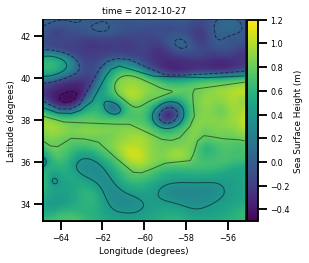
\includegraphics[trim={0 13mm 22mm 0},clip, width=3.60cm,height=3.2cm]{00_Oceanbench/content/figures/fourdvarnet_figs/osse_gf_nadir_ssh.png} &
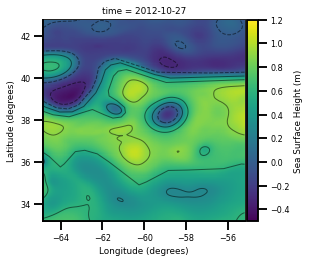
\includegraphics[trim={13mm 13mm 22mm 0},clip, width=3.2cm,height=3.2cm]{00_Oceanbench/content/figures/fourdvarnet_figs/osse_gf_nadirswot_ssh.png} &
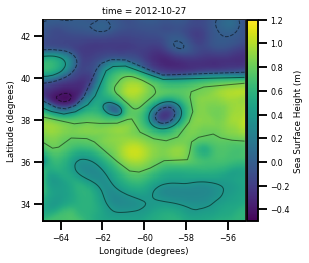
\includegraphics[trim={13mm 13mm 22mm 0},clip, width=3.2cm,height=3.2cm]{00_Oceanbench/content/figures/fourdvarnet_figs/osse_gf_nadir_sst_ssh.png} &
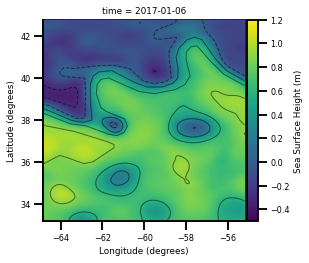
\includegraphics[trim={13mm 13mm 0 0},clip,width=4.0cm,height=3.2cm]{00_Oceanbench/content/figures/fourdvarnet_figs/ose_gf_ssh.png} \\
%\vspace{3mm}
%%%%% KINETIC ENERGY %%%%%%%%
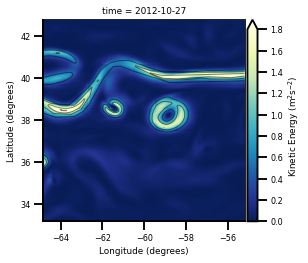
\includegraphics[trim={0 13mm 22mm 5mm}, clip, width=3.60cm,height=3cm]{00_Oceanbench/content/figures/fourdvarnet_figs/osse_gf_nadir_ke.png} &
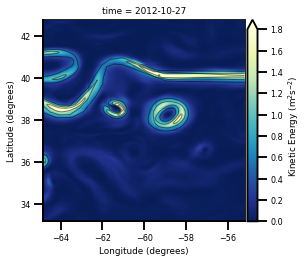
\includegraphics[trim={13mm 13mm 22mm 5mm},clip, width=3.2cm,height=3cm]{00_Oceanbench/content/figures/fourdvarnet_figs/osse_gf_nadirswot_ke.png} &
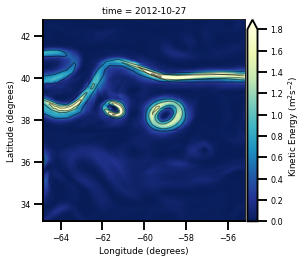
\includegraphics[trim={13mm 13mm 22mm 5mm},clip, width=3.2cm,height=3cm]{00_Oceanbench/content/figures/fourdvarnet_figs/osse_gf_nadir_sst_ke.png} &
\includegraphics[trim={13mm 13mm 0 5mm},clip,width=4cm,height=3cm]{00_Oceanbench/content/figures/fourdvarnet_figs/ose_gf_ke.png} \\
%%%%% RELATIVE VORTICITY %%%%%%%%
\includegraphics[trim={0 13mm 21.2mm 5mm},clip, width=3.60cm,height=3cm]{00_Oceanbench/content/figures/fourdvarnet_figs/osse_gf_nadir_vort_r.png} &
\includegraphics[trim={13mm 13mm 21.2mm 5mm},clip, width=3.2cm,height=3cm]{00_Oceanbench/content/figures/fourdvarnet_figs/osse_gf_nadirswot_vort_r.png} &
\includegraphics[trim={13mm 13mm 21.2mm 5mm},clip, width=3.2cm,height=3cm]{00_Oceanbench/content/figures/fourdvarnet_figs/osse_gf_nadir_sst_vort_r.png} &
\includegraphics[trim={13mm 13mm 0 5mm},clip,width=4.0cm,height=3cm]{00_Oceanbench/content/figures/fourdvarnet_figs/ose_gf_vort_r.png} \\
%%%%% STRAIN %%%%%%%%
\includegraphics[trim={0 0 19mm 5mm},clip, width=3.60cm,height=3.4cm]{00_Oceanbench/content/figures/fourdvarnet_figs/osse_gf_nadir_strain.png} &
\includegraphics[trim={13mm 0 19mm 5mm},clip, width=3.2cm,height=3.4cm]{00_Oceanbench/content/figures/fourdvarnet_figs/osse_gf_nadirswot_strain.png} &
\includegraphics[trim={13mm 0 19mm 5mm},clip, width=3.2cm,height=3.4cm]{00_Oceanbench/content/figures/fourdvarnet_figs/osse_gf_nadir_sst_strain.png} &
\includegraphics[trim={13mm 0 0 5mm},clip,width=4.0cm,height=3.4cm]{00_Oceanbench/content/figures/fourdvarnet_figs/ose_gf_strain.png} \\
% \vspace{-2mm}
(a) & (b) & (c) & (d)
\end{tabular}}
\vspace{-3mm}
% \caption{Row I - Isotrophic PSD. Row 2 - Isotrophic PSD Score}
\caption{
Reconstructed quantities by the 4dVarNet method for each of the four tasks.
Each row showcases the following physical variables found in appendix~\ref{sec:physical_variables}: (a) Sea Surface Height, (b) Kinetic Energy, (c) Relative Vorticity, and (d) Strain. 
Each column showcase the reconstructed from the tasks (a) OSSE using only Nadir tracks: (b) OSSE using Nadir tracks and SWOT swath, (c) Multimodal using Nadir tracks and sea surface temperature, and (d) Reconstruction using real nadir altimetry tracks.}
\label{fig:oceanbench_maps_4dvarnet}
\vspace{-5mm}
\end{center}
\end{figure}



\subsection*{\texttt{OceanBench} Pipelines}

% \begin{table}[h]
% \caption{This table highlights some of the results for the \textbf{OSSE NADIR} experiment outlined in section~\ref{sec:data_challenges} and appendix~\ref{sec:data_challenges_extended}.
% % and the OSE experiment outlined in section~\ref{sec:ose}~\tocite{}. 
% % For more results regarding the SWOT data, please see section~\ref{sec:other_tasks}. 
% This table highlights the performance statistically in the real and spectral space; the normalized RMSE score for the real space and the minimum spatial and temporal scales resolved in the spectral domain. 
% For more information about the class of models displayed and class of metrics, see appendix~\ref{sec:ml_ontology} and appendix~\ref{sec:metrics} respectively. We only showcase the model performance on the alongtrack NADIR data available. For the extended table for each of the challenges, see Table~\ref{tb:exp-results-mega}.}
% \label{tb:oceanbench_results}
% \centering
% \makebox[\textwidth]{
% \begin{tabular}{lllcccc}
%  \toprule
% % Experiment & Configuration & Method & nRMSE & Resolved Scale [km]    \\ \midrule
% % \multirow{2}{*}{Experiment} & \multirow{2}{*}{Algorithm} & \multirow{2}{*}{Algorithm Class} & \multirow{2}{*}{nRMSE} & \multicolumn{2}{c}{Effective Resolution} \\ 
% % &  &   &  & Wavelength [km]  & Period [days]      \\ \midrule
% % \multirow{2}{*}{Experiment} & \multirow{2}{*}{Algorithm} & \multirow{2}{*}{Algorithm Class} & \multirow{2}{*}{nRMSE} & \multicolumn{2}{c}{Effective Resolution} \\ 
% Experiment &  Algorithm &   Algorithm Class &  nRMSE Score & $\lambda_{\mathbf{x}}$ [km]  & $\lambda_{t}$ [days]      \\ \midrule
% \multicolumn{1}{l}{OSSE NADIR}     &  OI~\cite{DUACS} &  Coordinate-Based & 0.92 $\pm$ 0.01 & 175 & 10.8 \\
% \multicolumn{1}{l}{OSSE NADIR}     &  MIOST~\cite{MIOST} &  Coordinate-Based  & 0.93 $\pm$ 0.01 & 157 & 10.1 \\
% \multicolumn{1}{l}{OSSE NADIR}     &  BFNQG~\cite{BFNQG} &  Hybrid Model   & 0.93 $\pm$ 0.01 & 139 & 10.6 \\
% OSSE NADIR &  4DVarNet~\cite{4DVARNETSWOT} &  Bi-Level Opt.  & 0.95 $\pm$ 0.01 & 117 & 7.7 \\
% \bottomrule
% \end{tabular}}
% \end{table}



For the four data challenges presented in the previous section, we used \texttt{OceanBench} pipelines to deliver a ML-ready benchmarking framework.
We used the \texttt{hydra} and the geoprocessing tools outlined in section~\ref{sec:code_structure} with specialized routines for regridding the ocean satellite data to a uniformly gridded product and vice versa when necessary. 
Appendix~\ref{sec:hydra_recipes} showcases an example of the hydra integration for the preprocessing pipeline. 
A key feature is the creation of a custom patcher for the appropriate geophysical variables using our \texttt{XRPatcher} tool, which is later integrated into custom datasets and dataloaders for the appropriate model architecture, e.g., coordinate-based or grid-based. 
We provide an example snippet of how this can be done easily in section~\ref{sec:xrpatcher}.
\texttt{OceanBench} also features some tools specific to the analysis of SSH. 
For example, physically-interpretable variables like geostrophic currents and relative vorticity, which can be derived from first-order and second-order derivatives of the SSH, are essential for assessing the quality of the reconstructions generated by the models. 
Figure~\ref{fig:oceanbench_maps} showcases some fields of the most common physical variables used in the oceanography literature for the SSH-based analysis of sea surface dynamics.



% \begin{figure}[ht!]
\small
\begin{center}
\setlength{\tabcolsep}{1pt}
\begin{tabular}{cccc}
\hspace{3mm} Task OSSE & 
\hspace{3mm} Task OSSE & 
\hspace{2mm} Task OSSE & 
Task OSE \\
\hspace{3mm}  Nadir & 
\hspace{3mm} Nadir + SWOT & 
\hspace{2mm} Nadir + SST & 
Nadir \\
%\vspace{-2mm}
%%%%% SSH %%%%%%%%
\includegraphics[trim={0 13mm 22mm 0},clip, width=3.60cm,height=3.2cm]{content/figures/fourdvarnet_figs/osse_gf_nadir_ssh.png} &
\includegraphics[trim={13mm 13mm 22mm 0},clip, width=3.2cm,height=3.2cm]{content/figures/fourdvarnet_figs/osse_gf_nadirswot_ssh.png} &
\includegraphics[trim={13mm 13mm 22mm 0},clip, width=3.2cm,height=3.2cm]{content/figures/fourdvarnet_figs/osse_gf_nadir_sst_ssh.png} &
\includegraphics[trim={13mm 13mm 0 0},clip,width=4.0cm,height=3.2cm]{content/figures/fourdvarnet_figs/ose_gf_ssh.png} \\
%\vspace{3mm}
%%%%% KINETIC ENERGY %%%%%%%%
\includegraphics[trim={0 13mm 22mm 5mm}, clip, width=3.60cm,height=3cm]{content/figures/fourdvarnet_figs/osse_gf_nadir_ke.png} &
\includegraphics[trim={13mm 13mm 22mm 5mm},clip, width=3.2cm,height=3cm]{content/figures/fourdvarnet_figs/osse_gf_nadirswot_ke.png} &
\includegraphics[trim={13mm 13mm 22mm 5mm},clip, width=3.2cm,height=3cm]{content/figures/fourdvarnet_figs/osse_gf_nadir_sst_ke.png} &
\includegraphics[trim={13mm 13mm 0 5mm},clip,width=4cm,height=3cm]{content/figures/fourdvarnet_figs/ose_gf_ke.png} \\
%%%%% RELATIVE VORTICITY %%%%%%%%
\includegraphics[trim={0 13mm 21.2mm 5mm},clip, width=3.60cm,height=3cm]{content/figures/fourdvarnet_figs/osse_gf_nadir_vort_r.png} &
\includegraphics[trim={13mm 13mm 21.2mm 5mm},clip, width=3.2cm,height=3cm]{content/figures/fourdvarnet_figs/osse_gf_nadirswot_vort_r.png} &
\includegraphics[trim={13mm 13mm 21.2mm 5mm},clip, width=3.2cm,height=3cm]{content/figures/fourdvarnet_figs/osse_gf_nadir_sst_vort_r.png} &
\includegraphics[trim={13mm 13mm 0 5mm},clip,width=4.0cm,height=3cm]{content/figures/fourdvarnet_figs/ose_gf_vort_r.png} \\
%%%%% STRAIN %%%%%%%%
\includegraphics[trim={0 0 19mm 5mm},clip, width=3.60cm,height=3.4cm]{content/figures/fourdvarnet_figs/osse_gf_nadir_strain.png} &
\includegraphics[trim={13mm 0 19mm 5mm},clip, width=3.2cm,height=3.4cm]{content/figures/fourdvarnet_figs/osse_gf_nadirswot_strain.png} &
\includegraphics[trim={13mm 0 19mm 5mm},clip, width=3.2cm,height=3.4cm]{content/figures/fourdvarnet_figs/osse_gf_nadir_sst_strain.png} &
\includegraphics[trim={13mm 0 0 5mm},clip,width=4.0cm,height=3.4cm]{content/figures/fourdvarnet_figs/ose_gf_strain.png} \\
% \vspace{-2mm}
(a) & (b) & (c) & (d)
\end{tabular}
\vspace{-3mm}
% \caption{Row I - Isotrophic PSD. Row 2 - Isotrophic PSD Score}
\caption{
Reconstructed quantities by the 4dVarNet method for each of the four tasks.
Each row showcases the following physical variables found in appendix~\ref{sec:physical_variables}: (a) Sea Surface Height, (b) Kinetic Energy, (c) Relative Vorticity, and (d) Strain. 
Each column showcase the reconstructed from the tasks (a) OSSE using only Nadir tracks: (b) OSSE using Nadir tracks and SWOT swath, (c) Multimodal using Nadir tracks and sea surface temperature, and (d) Reconstruction using real nadir altimetry tracks.}
\vspace{-5mm}
\label{fig:oceanbench_maps_4dvarnet}
\end{center}
\end{figure}


\begin{table}[H]
% \caption{This table highlights some of the results for the OSSE experiments outlined in section~\ref{sec:osse} and~\ref{sec:other_tasks}.

% This table highlights the performance statistically in the real and spectral space; the normalized RMSE for the real space and the minimum spatial and temporal scales resolved in the spectral domain. 
% For more information about the class of models displayed and class of metrics, see section~\ref{sec:ml_ontology} and section~\ref{sec:metrics} respectively.}
\label{tb:exp-results-mega}
\centering
\makebox[\textwidth]{
\begin{tabular}{llcccccc}
 \toprule
% Experiment & Configuration & Method & nRMSE & Resolved Scale [km]    \\ \midrule
% \multirow{2}{*}{Experiment} & \multirow{2}{*}{Algorithm} & \multirow{2}{*}{Algorithm Class} & \multirow{2}{*}{nRMSE} & \multicolumn{2}{c}{Effective Resolution} \\ 
% &  &   &  & Wavelength [km]  & Period [days]      \\ \midrule
% \multirow{2}{*}{Experiment} & \multirow{2}{*}{Algorithm} & \multirow{2}{*}{Algorithm Class} & \multirow{2}{*}{nRMSE} & \multicolumn{2}{c}{Effective Resolution} \\ 
\multirow{2}{*}{Experiment} &  \multirow{2}{*}{Algorithm} &   \multirow{2}{*}{nRMSE Score} &
\multicolumn{4}{c}{Effective Resolution} \\
& & & $\lambda_{a}$ [km] & $\lambda_{r}$ [km]   &  $\lambda_{\mathbf{x}}$ [km]  &   $\lambda_{t}$ [days]      \\ \midrule
OSSE NADIR     &  OI & 0.92 & - & 123 & 174 & 10.8 \\
OSSE NADIR     &  MIOST &  0.93 & - & 100 & 157 & 10.1 \\
OSSE NADIR     &  BFNQG & 0.93 & - & 88 & 139 & 10.4 \\
OSSE NADIR &  4DVarNet &  \textbf{0.94} & - & \textbf{65} & \textbf{117} & \textbf{7.7} \\
\midrule
OSSE SWOT     &  OI & 0.92 & - & 106 & 139 & 11.7 \\
OSSE SWOT     &  MIOST &  0.94 & - & 88 & 131 & 10.1 \\
OSSE SWOT     &  BFNQG & 0.94 & - & 64 & 118 & 36.5 \\
OSSE SWOT &  4DVarNet &  \textbf{0.96} & - & \textbf{47} & \textbf{77} & \textbf{5.6} \\
\midrule
OSSE SST     &  Musti & 0.95 & - & 46 & 138 & 4.1 \\
OSSE SST &  4DVarNet &  \textbf{0.96} & - & \textbf{46} & \textbf{87} & \textbf{3.7} \\
\midrule
OSE NADIR     &  OI & 0.88 & 151 & - &  - &  -\\
OSE NADIR     &  MIOST &  0.90 & 135 & - &  - &  -\\
OSE NADIR     &  BFNQG & 0.88 & 122 & - & - &  -\\
OSE NADIR &  ConvLSTM &  0.89 & 113 &- &  - &  -\\
OSE NADIR &  4DVarNet & \textbf{0.91} & \textbf{98} & - &  -  &  -\\
\bottomrule
\end{tabular}}
\caption{This table showcases all of the summary statistics for some methods for each of the data challenges listed in section~\ref{sec:data_challenges}. The summary statistics shown are the normalized RMSE and the effective resolution in the spectral domain. The spectral metrics for the effective resolution that were outlined in section~\ref{sec:metrics} are: i) $\lambda_a$ is the spatial score for the alongtrack PSD score, ii) $\lambda_r$ is the spatial score for the isotropic PSD, iii) $\lambda_x$ is the spatial score for space-time PSD score, and iv) $\lambda_t$ is the temporal score for the space-time PSD score.}
\end{table}



%The \textit{Ocean-Data-Challenge} group has a wide-range of different OSSE and OSE experiments involving SSH interpolation in particular~\cite{DCOSEGULFSSH,DCOSSEGULFSSH}. 
%For this paper, we will focus on a subset and demonstrate some evaluation steps generated from the \texttt{OceanBench} framework.
%We outline an experimental setup SSH reconstruction over the Gulfstream with three OSSE's configurations and one OSE configuration in the next section. For more detailed information about the experimental setups for each configuration, see section~\ref{sec:data_challenges_extended} in the appendix.

% \begin{itemize}
%     \item 


%The observation data uses NADIR altimetry tracks which are very fine, thin ocean satellite observations (see Figure~\ref{fig:oceanbench_maps} (a) \& (b)). 





% \begin{itemize}
%     \item Experiment I (\textbf{OSSE NADIR}) addresses SSH interpolation using NADIR altimetry tracks which are very fine, thin ocean satellite observations (see Figure~\ref{fig:oceanbench_maps}). It relies on an OSSE using anocean simulations generated by the NEMO model, more precisely a high-resolution simulation, $1/60^\circ$ resolution, over one year with a whole field every day. 
% %The observation data uses NADIR altimetry tracks which are very fine, thin ocean satellite observations (see Figure~\ref{fig:oceanbench_maps} (a) \& (b)). 
% \item Experiment II (\textbf{OSSE SWOT}) addresses SSH interpolation using jointly NADIR and SWOT altimetry data. We complement the \textbf{OSSE NADIR} configuration with simulated SWOT observations.  
% SWOT is a new satellite altimetry mission with  much higher spatial coverage but a much lower temporal resolution as illustrated in Figure~\ref{fig:oceanbench_maps}.
% The higher spatial resolution allows us to see structures at a smaller resolution but at the cost of a massive influx of observations (over $\times 100$).
% \item Experiment III (\textbf{OSSE SST}) addresses SSH interpolation using 
% jointly altimetry and SST satellite data. We complement the \textbf{OSSE SWOT} challenge with simulated SST observations. 
% Satellite-derived SST observations are more abundantly available in natural operational settings than SSH at a finer resolution, and structures have visible similarities \cite{}.
% So this challenge allows for methods to take advantage of multi-modal learning \cite{}.
% \item Experiment IV \textbf{OSE NADIR} addresses SSH interpolation for real NADIR altimetry data. In contrast to the three OSSE data challenges, it only looks at actual observations aggregated from the currently available ocean altimetry data from actual satellites. It involves a similar space-time sampling as Experiment (\textbf{OSSE NADIR}) to evaluate the generalization of ML methods trained in Experiment I to real altimetry data. Besides, one may also explore learning or fine-tuning strategies from the available OSE dataset. We may point out that the complexity of the training problem due to the sparsity of refence dataset compared with \textbf{OSSE NADIR} dataset.
% \end{itemize}




Regarding the evaluation framework, we include domain-relevant performance metrics beyond the standard ML loss and accuracy functions. They account for the sampling patterns of the evaluation data. Spectral analytics are widely used in geoscience~\cite{BFNQG}, and here, we consider spectral scores computed as the minimum spatial and temporal scales resolved by the reconstruction methods proposed in~\cite{BFNQG}.
For example, figure~\ref{fig:oceanbench_psd} showcases how \texttt{OceanBench} generated the isotropic power spectrum and score and the space-time power spectrum decomposition and score.
Table~\ref{tb:oceanbench_results} outlines some standard and domain-specific scores for the experiments outlined in section~\ref{sec:experimental_design}.


% \begin{table}[h]
% \caption{This table highlights some of the results for the \textbf{OSSE NADIR} experiment outlined in section~\ref{sec:data_challenges} and appendix~\ref{sec:data_challenges_extended}.
% % and the OSE experiment outlined in section~\ref{sec:ose}~\tocite{}. 
% % For more results regarding the SWOT data, please see section~\ref{sec:other_tasks}. 
% This table highlights the performance statistically in the real and spectral space; the normalized RMSE for the real space and the minimum spatial and temporal scales resolved in the spectral domain. 
% For more information about the class of models displayed and class of metrics, see appendix~\ref{sec:ml_ontology} and appendix~\ref{sec:metrics} respectively. We only showcase the model performance on the alongtrack NADIR data available. For the extended table for each of the challenges, see Table~\ref{tb:exp-results-mega}.}
% \label{tb:oceanbench_results}
% \centering
% \begin{tabular}{lllcccc}
%  \toprule
% % Experiment & Configuration & Method & nRMSE & Resolved Scale [km]    \\ \midrule
% % \multirow{2}{*}{Experiment} & \multirow{2}{*}{Algorithm} & \multirow{2}{*}{Algorithm Class} & \multirow{2}{*}{nRMSE} & \multicolumn{2}{c}{Effective Resolution} \\ 
% % &  &   &  & Wavelength [km]  & Period [days]      \\ \midrule
% % \multirow{2}{*}{Experiment} & \multirow{2}{*}{Algorithm} & \multirow{2}{*}{Algorithm Class} & \multirow{2}{*}{nRMSE} & \multicolumn{2}{c}{Effective Resolution} \\ 
% Experiment &  Algorithm &   Algorithm Class &  nRMSE & $\lambda_{\mathbf{x}}$ [km]  & $\lambda_{t}$ [days]      \\ \midrule
% \multicolumn{1}{l}{OSSE NADIR}     &  OI (app.~\ref{sec:oi}) &  Coordinate-Based & 0.91 $\pm$ 0.01 & 176 & 11.6\\
% \multicolumn{1}{l}{OSSE NADIR}     &  MIOST~\ &  Coordinate-Based  & 0.92 $\pm$ 0.01 & 157 & 10.3 \\
% % \multicolumn{1}{l}{OSSE Gulf}     &  NerF &  Coordinate-Based  & 0.92 $\pm$ 0.01 & ... &\\
% \multicolumn{1}{l}{OSSE NADIR}     &  BFNQG (app.~\ref{sec:bfn}) &  Hybrid Model   & 0.92 $\pm$ 0.01 & 139 & 10.6 \\
% OSSE NADIR &  4DVarNet (app.~\ref{sec:4dvarnet}) &  Bi-Level Opt.  & 0.95 $\pm$ 0.01 & 117 & 7.7 \\
% % \bottomrule
% % OSE Gulf     &  OI &  Coordinate-Based  & ... & ... &\\
% % \multicolumn{1}{l}{OSE Gulf}     &  MIOST &  Coordinate-Based  & ... & ... &\\
% % \multicolumn{1}{l}{OSE Gulf}     &  NerF &  Coordinate-Based  & ... & ... &\\
% % \multicolumn{1}{l}{OSE Gulf}     &  BFNQG &  Hybrid Model  & ... & ... &\\
% % \multicolumn{1}{l}{OSE Gulf}     &  4DVarNet &  Bi-Level Opt.  & ... & ... &\\
% \bottomrule
% \end{tabular}
% \end{table}


\section{Discussion} \label{sec:conclusions}
\subsection*{Framework Limitations}

While we have advertised \texttt{OceanBench} as a unifying framework that provides standardized processing steps that comply with domain-expert standards, we also highlight some potential limitations that could hinder its adoption for the wider community.

\textbf{Data Serving}. We provide a few datasets but we omit some of the original simulations. We found that the original simulations are terabytes/petabytes of data which becomes infeasible for most modest users (even with adequate CPU resources).  
This is very big problem and if we want to have a bigger impact, we may need to do more close collaborations with specified platforms like the Marine Data Store~\citep{MDSOCEANPHYSICS,MDSBIOGEOCHEMICAL,MDSOCEANPHYSICSENS,MDSINSITU,MDSWAVES,MDSALONGTRACK,MDSSSH} or the Climate Data Store~\citep{CDSREANALYSISSST,CDSOBSSST,CDSOBSOC,CDSOBSSSTENS}. Furthermore, there are many people that will not be able to do a lot of heavy duty research which indirectly favours institutions with adequate resources and marginalizing others. 
This is also problematic as those communities tend to be the ones who need the most support from the products of such frameworks.
We hope that leaving this open-source at least ensure that the knowledge is public.

\textbf{Framework Dependence}. The user has to "buy-into" the \texttt{hydra} framework to really take advantage of \texttt{OceanBench}. This adds a layer of abstraction and a new tool to learn. 
However, we designed the project so that high level usage does not require in-depth knowledge of the framework. 
In addition, we hope that, despite the complexity of project, users will appreciate the flexibility and extensibility of this framework.


\textbf{Lack of Metrics}. We do not provide the most exhaustive list of metrics available with the ocean community. In fact, we also believe that many of these metrics are often poor and do not effectively assess the goodness of our reconstructions. 
However, we do provide a platform that will hopefully be useful and easy to implement new and improved metrics.
Furthermore, having a wide range of metrics that are trusted across communities may help to improve the overall assessment of the different model performances~\cite{METRICSAVERAGE}.

\textbf{Limited ML Scope}. 
The framework does not support nor promote any machine learning methods and we lack any indication of comparing ML training and inference performance. 
However, we argue that a benchmark framework will allow us to effectively compare whichever ML methods are demonstratively the best which is a necessary preliminary step which offers users more flexibility in the long-run.

\textbf{Broad Oceans Application Scope}. 
We have targeted a broad ocean-application scope of state estimation.
However, there may be more urgent applications such as maritime monitoring, object tracking, and general ocean health.
However, we feel that many downstream applications require high-quality maps.
In addition, those downstream applications tend to be very complicated and are not always straightforward to apply ML under those instances.

\textbf{Full Pipeline Transparency}. We use a lot of different \texttt{xarray}-specific packages which have different design principles, assumptions and implementations. This may give the users an illusion of simplicity and transparency to real-world use. However, there are many underlying assumptions within each of the packages that may occlude a lot of design decisions.
Despite this limitation, we believe that being transparent about the processing steps and being consistent with the evaluation procedure will be beneficial for the ML research community.

\textbf{Scalability}. Scaling this to many terabytes or petabytes of data is easily the biggest limitation of the framework. In addition, we have only showcased demonstrations for 2D+T fields which are much less expensive than 3D+T fields.

\textbf{Deployability}. MLOPs has many wheels and it is not easy to integrate into existing systems. We offer no solutions to this. 
However, we believe that our framework is fully transparent in the assumptions and use cases which will facilitate some adoption into operational systems where they can further modify it for their use cases (see the evolution of \texttt{WeatherBench} and \texttt{ClimateBench}).

\textbf{Visualization Tools}.
We do not incorporate a high quality visualization tool that allows users to do pre- and post-analysis at a large scale. 
We do provide some simple visualization steps that are ML-relevant (see the GitHub repo) but it is very limited to ML standards.
One solution is to interface our pipeline with the source of many ocean datasets, e.g. Climate Data Store~\citep{CDSREANALYSISSST} or Marine Data Store~\citep{MDSOCEANPHYSICS}, then we can offset this task to them where they can offer better quality visualization tools.


\subsection*{Conclusion}
The ocean community faces technological and algorithmic challenges to make the most of available observation and simulation datasets. 
In this context, recent studies evidence the critical role of ML schemes in reaching breakthroughs in our ability to monitor ocean dynamics for various space-time scales and processes. 
Nevertheless, domain-specific preprocessing steps and evaluation procedures slow down the uptake of ML toward real-world applications. 
The application considered here is SSH mapping which facilities the production of many crucial derived products that are used in many downstream tasks like subsequent modeling~\citep{ML4OCN}, ocean health monitoring~\citep{ML4NATURECONSERVATION,OCNHEALTH,OCEANHEALTH2} and maritime risk assessment~\citep{SSHOPERATIONAL}.

We proposed four challenges towards a ML-ready benchmarking suite for ocean observation challenges. 
We outlined the inner workings \texttt{OceanBench} and demonstrated its usefulness by recreating some preprocessing and analysis pipelines from a few data challenges involving SSH interpolation.
We firmly believe that the \texttt{OceanBench} platform is instrumental in fostering greater ML method adoption by the ocean community, while also rallying a larger portion of the ML community to tackle the ocean's scientific complexities.




%% ACKNOWLEDGEMENTS
\newpage
% \begin{ack}
This work was supported by the French National Research Agency (ANR), through projects number ANR-17- CE01-0009-01, ANR-19-CE46-0011 and ANR-19-CHIA-0016); by the French National Space Agency (CNES) through the SWOT Science Team program (projects MIDAS and DIEGO) and the OSTST program (project DUACS-HR); by the French National Centre for Scientific Research (CNRS) through the LEFE-MANU program (project IA-OAC). This project also received funding from the European Union’s Horizon Europe research and innovation programme under the grant No 101093293 (EDITO-Model Lab project). This project benefited from HPC and GPU computing resources from GENCI-IDRIS (Grant 2021-101030).
\end{ack}
% \section*{Checklist}

% %%% BEGIN INSTRUCTIONS %%%
% The checklist follows the references.  Please
% read the checklist guidelines carefully for information on how to answer these
% questions.  For each question, change the default \answerTODO{} to \answerYes{},
% \answerNo{}, or \answerNA{}.  You are strongly encouraged to include a {\bf
% justification to your answer}, either by referencing the appropriate section of
% your paper or providing a brief inline description.  For example:
% \begin{itemize}
%   \item Did you include the license to the code and datasets? \answerYes{See Section~\ref{gen_inst}.}
%   \item Did you include the license to the code and datasets? \answerNo{The code and the data are proprietary.}
%   \item Did you include the license to the code and datasets? \answerNA{}
% \end{itemize}
% Please do not modify the questions and only use the provided macros for your
% answers.  Note that the Checklist section does not count towards the page
% limit.  In your paper, please delete this instructions block and only keep the
% Checklist section heading above along with the questions/answers below.
% %%% END INSTRUCTIONS %%%

\begin{enumerate}

\item For all authors...
\begin{enumerate}
  \item Do the main claims made in the abstract and introduction accurately reflect the paper's contributions and scope?
    \answerYes{All the contributions listed in the abstract are elaborated in sections~\ref{sec:code_structure},~\ref{sec:data_challenges} and~\ref{sec:conclusions}}
  \item Did you describe the limitations of your work?
    \answerYes{See the last paragraph of section 5 and the appendix as well.}
  \item Did you discuss any potential negative societal impacts of your work?
    \answerYes{We do not believe that our work has any potential negative societal impacts directly as we do not deal with any confidential or private data. However, we do outline in the appendix how there may be some adverse effects related to downstream uses which could have some negative societal impacts.}
  \item Have you read the ethics review guidelines and ensured that your paper conforms to them?
    \answerYes{We do not include any confidential or private data. We only include numerical values which stem from general physical systems or machine learning models. We do not believe they hold any ethical issues. However, we do acknowledge that there would be environmental damage should users go forward and explore methods which obscenely high computing hours. This discussion outlined in the appendix.}
\end{enumerate}

\item If you are including theoretical results...
\begin{enumerate}
  \item Did you state the full set of assumptions of all theoretical results?
    \answerNA{We do not include any theoretical results.}
	\item Did you include complete proofs of all theoretical results?
    \answerNA{We do not include any theoretical results.}
\end{enumerate}

\item If you ran experiments (e.g. for benchmarks)...
\begin{enumerate}
  \item Did you include the code, data, and instructions needed to reproduce the main experimental results (either in the supplemental material or as a URL)?
    \answerYes{We include the parameters used to reproduce the dataset preprocessing and evaluation procedure in Appendix \ref{sec:data_challenges_extended} and instructions are given to download the data via~\href{https://github.com/quentinf00/oceanbench-data-registry}{https://github.com/quentinf00/oceanbench-data-registry} and rerun the evaluation procedure in our code repository which is available at~\href{https://github.com/jejjohnson/oceanbench}{https://github.com/jejjohnson/oceanbench}.}
  \item Did you specify all the training details (e.g., data splits, hyperparameters, how they were chosen)?
    \answerYes{We showcase all preprocessing steps necessary to reproduce the experimental configurations in Appendix~\ref{sec:data_challenges_extended} and the configuration files are available in our code repository at~\href{https://github.com/jejjohnson/oceanbench}{https://github.com/jejjohnson/oceanbench}. }
	\item Did you report error bars (e.g., with respect to the random seed after running experiments multiple times)?
    \answerNA{This is not applicable for this instantiation because we do not include any randomness within the experiment procedure nor the results.}
	\item Did you include the total amount of compute and the type of resources used (e.g., type of GPUs, internal cluster, or cloud provider)?
    \answerYes{We do not do any model training and leave it up the user for their local or cloud machine. However, we do provide the cloud provider for the data found the the data registry which can be found at~\href{https://github.com/quentinf00/oceanbench-data-registry}{https://github.com/quentinf00/oceanbench-data-registry}}
\end{enumerate}

\item If you are using existing assets (e.g., code, data, models) or curating/releasing new assets...
\begin{enumerate}
  \item If your work uses existing assets, did you cite the creators?
    \answerYes{We adopted the implementation of the preprocessing procedures and evaluation steps with some modifications. We give proper citation and credit to the authors as well as all other existing software packages included in this work.}
  \item Did you mention the license of the assets?
    \answerYes{The appropriate license notices are included in the source code files.}
  \item Did you include any new assets either in the supplemental material or as a URL?
    \answerYes{All the processing and evaluation scripts are included in the GitHub repository.}
  \item Did you discuss whether and how consent was obtained from people whose data you're using/curating?
    \answerYes{We only include data that is already publicly available. We also discussed with the original generators of the datasets and keep the appropriate licenses.}
  \item Did you discuss whether the data you are using/curating contains personally identifiable information or offensive content?
    \answerNA{We do not include any personal information or offensive content in our datasets.}
\end{enumerate}

\item If you used crowdsourcing or conducted research with human subjects...
\begin{enumerate}
  \item Did you include the full text of instructions given to participants and screenshots, if applicable?
    \answerNA{We do not use crowdsourcing and we do not conduct research with human subjects.}
  \item Did you describe any potential participant risks, with links to Institutional Review Board (IRB) approvals, if applicable?
    \answerNA{See the previous point.}
  \item Did you include the estimated hourly wage paid to participants and the total amount spent on participant compensation?
    \answerNA{See the previous point.}
\end{enumerate}

\end{enumerate}

% \bibliographystyle{plain}
% \nocite{*}
% \documentclass{article}



% if you need to pass options to natbib, use, e.g.:
%     \PassOptionsToPackage{numbers, compress}{natbib}
% before loading neurips_data_2023

% ready for submission
% \usepackage{neurips_data_2023}
\usepackage[preprint]{neurips_data_2023}

% to compile a preprint version, add the [preprint] option, e.g.:
%     \usepackage[preprint]{neurips_data_2023}
% This will indicate that the work is currently under review.

% to compile a camera-ready version, add the [final] option, e.g.:
%     \usepackage[final]{neurips_data_2023}

% to avoid loading the natbib package, add option nonatbib:
%    \usepackage[nonatbib]{neurips_data_2023}

% Submissions to the datasets and benchmarks are typically non anonymous,
% but anonymous submissions are allowed. If you feel that you must submit 
% anonymously, you can compile an anonymous version by adding the [anonymous] 
% option, e.g.:
%     \usepackage[anonymous]{neurips_data_2023}
% This will hide all author names.

\usepackage{color}
\usepackage{soul}
\usepackage[dvipsnames]{xcolor}
\usepackage[normalem]{ulem}
\newcommand{\todo}[1]{\textcolor{BrickRed}{[\textbf{TODO}]} }
\newcommand{\tocite}[1]{\textcolor{Plum}{[\textbf{CITE}: #1]}}
\newcommand{\hlc}[2][yellow]{{%
    \colorlet{foo}{#1}%
    \sethlcolor{foo}\hl{#2}}%
}
\newcommand{\tofix}[1]{\hlc[red!20]{#1}}

\usepackage[utf8]{inputenc} % allow utf-8 input
\usepackage[T1]{fontenc}    % use 8-bit T1 fonts
\usepackage{hyperref}       % hyperlinks
\usepackage{url}            % simple URL typesetting
\usepackage{booktabs}       % professional-quality tables
\usepackage{nicefrac}       % compact symbols for 1/2, etc.
\usepackage{microtype}      % microtypography
\usepackage{xcolor}         % colors
\usepackage{multirow}
\usepackage{graphicx}

%% MATH PACKAGES
\usepackage{amsfonts}       % blackboard math symbols
\usepackage{amsmath}
\usepackage{nicefrac} 


\usepackage{listings}
% \usepackage{minted}
% \usepackage[cachedir=.]{minted}
% \usepackage{frozencache}
% \usepackage[frozencache=true,cachedir=minted]{minted} 
\usepackage[finalizecache=true,cachedir=minted-cache]{minted}
% \usepackage[cachedir=.]{minted}

% \usepackage{appendix}

% here is a macro expanding to the name of the language
% (handy if you decide to change it further down the road)

\newcommand\YAMLcolonstyle{\color{red}\mdseries}
\newcommand\YAMLkeystyle{\color{black}\bfseries}
\newcommand\YAMLvaluestyle{\color{blue}\mdseries}

\makeatletter

% here is a macro expanding to the name of the language
% (handy if you decide to change it further down the road)
\newcommand\language@yaml{yaml}

\expandafter\expandafter\expandafter\lstdefinelanguage
\expandafter{\language@yaml}
{
  keywords={true,false,null,y,n},
  keywordstyle=\color{darkgray}\bfseries,
  basicstyle=\YAMLkeystyle,                                 % assuming a key comes first
  sensitive=false,
  comment=[l]{\#},
  morecomment=[s]{/*}{*/},
  commentstyle=\color{purple}\ttfamily,
  stringstyle=\YAMLvaluestyle\ttfamily,
  moredelim=[l][\color{orange}]{\&},
  moredelim=[l][\color{magenta}]{*},
  moredelim=**[il][\YAMLcolonstyle{:}\YAMLvaluestyle]{:},   % switch to value style at :
  morestring=[b]',
  morestring=[b]",
  literate =    {---}{{\ProcessThreeDashes}}3
                {>}{{\textcolor{red}\textgreater}}1     
                {|}{{\textcolor{red}\textbar}}1 
                {\ -\ }{{\mdseries\ -\ }}3,
}

% switch to key style at EOL
\lst@AddToHook{EveryLine}{\ifx\lst@language\language@yaml\YAMLkeystyle\fi}
\makeatother

\newcommand\ProcessThreeDashes{\llap{\color{cyan}\mdseries-{-}-}}


\definecolor{codegreen}{rgb}{0,0.6,0}
\definecolor{codegray}{rgb}{0.5,0.5,0.5}
\definecolor{codepurple}{rgb}{0.58,0,0.82}
\definecolor{backcolour}{rgb}{0.95,0.95,0.92}

\lstdefinestyle{pythonstyle}{
    % backgroundcolor=\color{backcolour},   
    commentstyle=\color{codegreen},
    keywordstyle=\color{magenta},
    numberstyle=\tiny\color{codegray},
    stringstyle=\color{codepurple},
    basicstyle=\ttfamily\footnotesize,
    breakatwhitespace=false,         
    breaklines=true,                 
    captionpos=b,                    
    keepspaces=true,                 
    numbers=left,                    
    numbersep=5pt,                  
    showspaces=false,                
    showstringspaces=false,
    showtabs=false,                  
    tabsize=2
}

\lstset{style=pythonstyle}


\title{\textsc{OceanBench}: \\ The Sea Surface Height Edition}

% The \author macro works with any number of authors. There are two commands
% used to separate the names and addresses of multiple authors: \And and \AND.
%
% Using \And between authors leaves it to LaTeX to determine where to break the
% lines. Using \AND forces a line break at that point. So, if LaTeX puts 3 of 4
% authors names on the first line, and the last on the second line, try using
% \AND instead of \And before the third author name.

\author{%
  J. Emmanuel Johnson$^*$\\
%   MEOM/Institut des Géosciences de l’Environnement, UGA\\
  % Univ. Grenoble Alpes, CNRS UMR IGE, Grenoble, France\\
  CNRS UMR IGE \\
  \texttt{johnsonj@univ-grenoble-alpes.fr}\\
  % examples of more authors
  \And
  Quentin Febvre$^*$\\
  IMT Atlantique\\
  \texttt{quentin.febvre@imt-atlantique.fr} \\
  \And
  Anastasia Gorbunova\\
  CNRS UMR IGE \\
  % \texttt{gorbunoa@univ-grenoble-alpes.fr} \\
  \And
  Sammy Metref\\
  DATLAS\\
  % \texttt{metrefs@univ-grenoble-alpes.fr}\\
  \And
  Maxime Ballarotta\\
  CLS\\
  % \texttt{mballarotta@groupcls.com} \\
  \And
  Julien Le Sommer\\
  CNRS UMR IGE\\
  % \texttt{julien.lesommer@univ-grenoble-alpes.fr} \\
  \And
  Ronan Fablet\\
  IMT Atlantique \\
  % \texttt{ronan.fablet@imt-atlantique.fr} \\
}


% \author{%
%   David S.~Hippocampus\thanks{Use footnote for providing further information
%     about author (webpage, alternative address)---\emph{not} for acknowledging
%     funding agencies.} \\
%   Department of Computer Science\\
%   Cranberry-Lemon University\\
%   Pittsburgh, PA 15213 \\
%   \texttt{hippo@cs.cranberry-lemon.edu} \\
%   % examples of more authors
%   % \And
%   % Coauthor \\
%   % Affiliation \\
%   % Address \\
%   % \texttt{email} \\
%   % \AND
%   % Coauthor \\
%   % Affiliation \\
%   % Address \\
%   % \texttt{email} \\
%   % \And
%   % Coauthor \\
%   % Affiliation \\
%   % Address \\
%   % \texttt{email} \\
%   % \And
%   % Coauthor \\
%   % Affiliation \\
%   % Address \\
%   % \texttt{email} \\
% }


\begin{document}




\maketitle
\def\thefootnote{*}\footnotetext{These authors contributed equally to this work}\def\thefootnote{\arabic{footnote}}

%##################################
% KEYWORDS
% - Sea Surface Height
% - Interpolation
% - Inverse Problem
% - 
% Scientific Machine Learning
% Benchmark, Partial Differential Equations, PINN, FNO, U-Net, Inverse problem

% \begin{abstract}
% The ocean is a key component of the climate system, profoundly influencing human activities. Consequently, a central question for oceanographers revolves around its observation and prediction at different timescales. Similar to various research fields, oceanography has recently witnessed the emergence of machine learning-based methods as an alternative to more domain-specific approaches. But, surprisingly, the adoption of machine learning methods in this field has been arguably slower compared to others. This can be attributed to the complexity of pre-processing tasks in the domain of geospatial data and to the specialized nature of evaluation metrics relevant to ocean science problems. In this context, we introduce \texttt{OceanBench}, a framework designed to lower the barrier to entry for ML researchers by standardizing and automating this process that comply with domain-expert standards.
% It seeks to maintains readability, robustness, and flexibility by providing a standardized framework to explicitly highlight the preprocessing step used, the parameters chosen and the sequence of operations performed. 
% It takes a step towards incorporate these domain-driven decisions to integrate well with existing ML pipelines.
% We demonstrate the usefulness of \texttt{OceanBench} on a series of SSH interpolation tasks with consistent dataflow pipelines, physically-inspired metrics, and interpretable visualizations.

% \end{abstract}

  % The abstract paragraph should be indented \nicefrac{1}{2}~inch (3~picas) on
  % both the left- and right-hand margins. Use 10~point type, with a vertical
  % spacing (leading) of 11~points.  The word \textbf{Abstract} must be centered,
  % bold, and in point size 12. Two line spaces precede the abstract. The abstract
  % must be limited to one paragraph.

\begin{abstract}

The ocean is a crucial component of the Earth's system. 
It profoundly influences human activities and plays a critical role in climate regulation. 
Our understanding has significantly improved over the last decades with the advent of satellite remote sensing data, allowing us to capture essential sea surface quantities over the globe, e.g., sea surface height (SSH). 
Despite their ever-increasing abundance, ocean satellite data presents challenges for information extraction due to their sparsity and irregular sampling, signal complexity, and noise. 
Machine learning (ML) techniques have demonstrated their capabilities in dealing with large-scale, complex signals. 
Therefore we see an opportunity for these ML models to harness the full extent of the information contained in ocean satellite data. 
However, data representation and relevant evaluation metrics can be \textit{the} defining factors when determining the success of applied ML. 
The processing steps from the raw observation data to a ML-ready state and from model outputs to interpretable quantities require domain expertise, which can be a significant barrier to entry for ML researchers. 
In addition, imposing fixed processing steps, like committing to specific variables, regions, and geometries, will narrow the scope of ML models and their potential impact on real-world applications. 
\textbf{OceanBench} is a unifying framework that provides standardized processing steps that comply with domain-expert standards. 
It is designed with a flexible and pedagogical abstraction: it a) provides plug-and-play data and pre-configured pipelines for ML researchers to benchmark their models w.r.t. ML and domain-related baselines and b) provides a transparent and configurable framework for researchers to customize and extend the pipeline for their tasks. 
In this work, we demonstrate the \texttt{OceanBench} framework through a first edition dedicated to SSH interpolation challenges. 
We provide datasets and ML-ready benchmarking pipelines for the long-standing problem of interpolating observations from simulated ocean satellite data, multi-modal and multi-sensor fusion issues, and transfer-learning to real ocean satellite observations. 
The \texttt{OceanBench} framework is available at~\href{https://github.com/jejjohnson/oceanbench}{github.com/jejjohnson/oceanbench} and the dataset registry is available at~\href{https://github.com/quentinf00/oceanbench-data-registry}{github.com/quentinf00/oceanbench-data-registry}.

\end{abstract}


%%%%%%%%%%%%%%%%%%%%%%%%%%%%%%%%%%%%%%%%%%%%%%%%%%%%%%%%%%%%%%%%%%%%%%%%%%%%%%%%%%%%%%%%%%%%%%%%%%%%%%%%%%%%%%%%%%%%%%%%%%%%%%%%%%%%%%%%%%%%%%%%%

% - We demonstrate how \texttt{OceanBench} can be used as an underlying framework with a series of SSH interpolation tasks which combines different variables, regions and geometries. 


% Q - make use of everything we mentioned above!
% E/Q - we want to showcase that OceanBench can be used for SSH interpolation 
% - we want to demonstrate how we can design different experiments/modifications with minimal code changes
% Q - simple tasks SSH -> SSH; extend it a) add domain, b) include other variables, c) switching to real data
% - enrich a simple experimental setups with additional variations

%%%%%%%%%%%%%%%%%%%%%%%%%%%%%%%%%%%%%%%%%%%%%%%%%%%%%%%%%%%%%%%%%%%%%%%%%%%%%%%%%%%%%%%%%%%%%%%%%%%%%%%%%%%%%%%%%%%%%%%%%%%%%%%%%%%%%%%%%%%%%%%%%



%%%%%%%%%%%%%%%%%%%%%%%%%%%%%%%%%%%%%%%%%%%%%%%%%%%%%%%%%%%%%%%%%%%%%%%%%%%%%%%%%%%%%%%%%%%%%%%%%%%%%%%%%%%%%%%%%%%%%%%%%%%%%%%%%%%%%%%%%%%%%%%%%

% - There is some work to be done to get the observation data to a ML-ready state.
% - Deciding the appropriate transformations requires domain-expertise which can be a large barrier to entry for ML researchers.

% - ML methods cannot be applied out of the box on raw observation data because .. blah blah

% - Despite the potential of machine learning to solve the issues that plague geosciences, the barrier to entry for machine learning (ML) researchers in ocean sciences is often hindered by the vastly different schemes for preprocessing techniques required to get the geo-centric data to a ML-ready state.
% \texttt{OceanBench} is a framework for co-designing machine learning-driven high level data products from ocean observations. 
%%%%%%%%%
% Why dont we just provide the processed data and call it a day...?
% Q - 1) non-standardized preprocessing steps; 2) regional differences
% 1 - multiple ways to take advantage of the Obs data (covariates, coordinate-based, gridded)
% Keeping the flexibilities allow for extensibility and multiple 
%%%%%%%%%%%%$
% 1 - OceanBench is a unifying framework that provides standardized processing steps that comply with domain-expert standards.
% 2 - It is designed for - flexible, padagological, abstract, :
% a - getting ML researchers quickly involved (data + preconfigured pipelines -> ML ready setups and test their models)
% - provides data and preconfigured pipelines for ML researchers to quickly experiment with different setups,
% - transparent and configurable for researchers to customize and extend the pipeline for their own objectives
% b - pedagological, unified setup to create and modified tasks (extensible)
% - flexibility
% 3 - We demonstrate ho
% %
% \texttt{OceanBench} is a framework that standardizing ... these processing steps that comply with domain-expert standards.
% %
% It is designed to lower the barrier to entry for ML researchers by providing preconfigured pipelines, ... "one-stop-shop for it all", and providing illustrative examples for different audiences.
% * 
% * provide a common interface for the processing steps
% * create a few ML tasks from raw data to ML ready using the above steps
% * showcase how one can orchestrate preconfigured pipelines to create a variety of ML tasks
% * preconfigured pipelines to illustrate example applications

% 1 - getting ML researchers quickly involved (data + preconfigured pipelines -> ML ready setups and test their models)
% 2 - pedagological, unified setup to create and modified tasks

% %%%%%
% \texttt{OceanBench} is a framework 
% - lower the barrier to entry
% - accessibility
% - one place to look to get all the stuff you want to do
% - preconfigured pipelines
% - jbooks with illustrated examples.
% - standardized preprocessing steps.
%
% It seeks to maintains readability, robustness, and flexibility by providing a standardized framework to explicitly highlight the preprocessing step used, the parameters chosen and the sequence of operations performed. 
%
% It takes a step towards incorporate these domain-driven decisions to integrate well with existing ML pipelines.
%
% We demonstrate the usefulness of \texttt{OceanBench} on a series of SSH interpolation tasks with 
% consistent dataflow pipelines, physically-inspired metrics, and interpretable visualizations.
\section{Motivation}

The ocean is vital to the Earth's system~\cite{OCEANWARMING}. 
It plays a significant role in climate regulation regarding carbon~\cite{OCEANCARBONCYCLE} and heat uptake~\cite{OCEANHEATUPTAKE}. It is also a primary driver of human activities (e.g., maritime traffic and world trade, marine resources and services)~\cite{SSHOPERATIONAL, ML4OCN}. 
However, monitoring the ocean is a critical challenge: the ocean state can only partially be determined because most of the ocean consists of subsurface quantities that we cannot directly observe. 
Thus, to quantify even a fraction of the physical or biochemical ocean state, we must often rely only on surface quantities that we can monitor from space, drifting buoys, or autonomous devices.
Satellite remote sensing, in particular, is one of the most effective ways of measuring essential sea surface quantities~\cite{Altimetry} such as sea surface height (SSH)~\cite{DUACS}, sea surface temperature (SST)~\cite{OCEANSATELLITESST}, and ocean color (OC)~\cite{OCEANSATELLITEOC}. 
While these variables characterize only a tiny portion of the ocean ecosystem, they present a gateway to many other derived physical quantities~\cite{ML4OCN}.


% satellite-derived SSH data allow us to monitor the sea level rise as well as critical physical and biogeochemical ocean processes,
Although we can access observable sea surface quantities, they are generally irregularly and extremely sparsely sampled. 
For instance, satellite-derived SSH data has less than 5\% coverage of the globe daily~\cite{DUACS}. 
These sampling gaps make the characterization of ocean processes highly challenging for operational products and downstream tasks that depend on relevant gap-free variables. This has motivated a rich literature in geoscience over the last decades, mainly using geostatistical kriging methods \cite{DUACS, MIOST} and model-driven data assimilation schemes~\cite{BFNQG, GLORYS12}. Despite significant progress, these schemes often need to improve their ability to leverage available observation datasets' potential fully. 
This has naturally advocated for exploring data-driven approaches like shallow ML schemes~\cite{DINEOF, DINEOF2, ANALOGDA2, ANALOGDA}. Very recently, deep learning schemes \cite{SSHInterpAttention, SSHInterpConvLSTM, SSHInterpUNet} have become appealing solutions to benefit from existing large-scale observation and simulation datasets and reach significant breakthroughs in the monitoring of upper ocean dynamics from scarcely and irregularly sampled observations. However, the heterogeneity and characteristics of the observation data present major challenges for effectively applying these methods beyond idealized case studies. 
A data source could have different variables, geometries, and noise levels, resulting in many domain-specific preprocessing procedures that can vastly change the solution outcome.
Furthermore, the evaluation procedure of the methods and their effectiveness can be regionally-dependent as the physical phenomena vary in space and time, which adds another layer of complexity in convincing domain scientists of their trustworthiness.
So the entire ML pipeline now requires a unified framework for dealing with heterogeneous data sources, different pre- and post-processing methodologies, and regionally-dependent evaluation procedures.

 %So the nature of the observations presents a key challenge for operational products and downstream tasks that depend on relevant gap-free variables.
%In addition, this sparsity 
%Although methods like smoothers~\tocite{OI, MIOST}, data assimilation~\tocite{BFN} and machine learning (ML)~\tocite{NerFs,recent-stuff, Ronan} have produced viable solutions to filling the gaps in ocean satellite, the heterogeneity and characteristics of the observation data present major challenges for effectively applying these methods. 
% No model nor observation systems captures all scales and processes.
% Operational methods like optimal interpolation and data assimilation ...
% Thus, there is a need for better model/data integration schemes that fully benefit from HR models and ever-increasing observation datasets.

% \textbf{Opportunity}.
%An end-to-end framework for piping data from its raw form to an ML-ready state and from model outputs to interpretable quantities is challenging. Designing an effective system that does this is the basis for many MLOPs tools and research~\tocite{MLOPs Research}.
To address these challenges, we introduce \textbf{OceanBench}, a framework for co-designing machine-learning-driven high-level experiments from ocean observations. 
It consists of an end-to-end framework for piping data from its raw form to an ML-ready state and from model outputs to interpretable quantities. 
We regard \texttt{OceanBench} as a key facilitator for the uptake of MLOPs tools and research~\cite{MLOPS1,MLOPS2} for ocean-related datasets and case studies. This first edition provides datasets and ML-ready benchmarking pipelines for SSH interpolation problems, an essential topic for the space oceanography community, related to ML communities dealing with issues like in-painting~\cite{InPaintingSurvey}, denoising~\cite{DENOISESURVEY,DENOISESURVEY2}, and super-resolution~\cite{SuperResSurvey}. 
We expect \texttt{OceanBench} to facilitate new challenges to the applied machine learning community and contribute to meaningful ocean-relevant breakthroughs.
%
The remainder of the paper is organized as follows: in \S2, we outline some related work that was inspirational for this work; in \S3, we formally outline \texttt{OceanBench} by highlighting the target audience, code structure, and problem scope; in \S4, we outline the problem formulation of SSH interpolation and provide some insight into different tasks related to SSH interpolation where \texttt{OceanBench} could provide some helpful utility; and in \S5 we give some concluding remarks while also informally inviting other researchers to help fill in the gaps.

% \textbf{How We Measure SSH + Gap Problem}. 




% % \textbf{Data Deluge, Gaps, \& ML Integration}. 
% Like most geosciences, the ocean sciences also suffer from the data deluge that persists due to the large amounts of observed quantities being collected daily~\tocite{Gus}. 
% The increased availability and quantity of observations are beneficial because it offers the community more insight into the physical processes at a finer resolution.
% % Consequently, this can help oceanographers revolve a central question of observing and predicting the ocean state at different spatial and timescales. 
% The trade-off is that processing this data is very expensive.
% Furthermore, it is impossible to accurately measure the entire globe concurrently, resulting in data with many gaps.
% Many operational systems have historically used ad-hoc coordinate-based schemes to gap-fill the data based on covariance assumptions. 
% However, with the abundance of new data~\tocite{SWOT}, these covariance-based schemes are reaching their limit due to the computational and signal complexity.
% Machine learning (ML) has been recently introduced as a viable alternative to filling the gaps in data where many classes of methods have found success, including coordinate-based methods~\tocite{OI,MIOST,NerFs}, direct surrogate/hybrid methods~\tocite{BFN, recent-stuff}, and end-to-end learning schemes~\tocite{Ronan}. 
% Nevertheless, most of these methods have only been applied to regions, and more needs to be applied at a large scale that comes close to the operational settings.


% % \textbf{Logistics Problem}.
% % \textbf{The Problem with Observation Data}.
% % The community is quickly facing a logistics problem.
% Dealing with complex problems such as SSH interpolation requires dealing directly with the observation data, often involving aggregating observations from satellites, buoys, or autonomous devices.
% In all cases, we can only observe a tiny portion of the Earth at any given time, resulting in highly sparse data (often <5\% coverage).
% This problem is even more difficult because the data sources are often heterogeneous, with different variables, geometries, and noise levels.
% Furthermore, the evaluation procedure can be regionally dependent as the physical phenomena vary globally. 
% So the entire ML pipeline now requires a unified framework for dealing with heterogeneous data sources, different pre- and post-processing methodologies, and regional dependent evaluation procedures.

% To solve a difficult problem such as SSH interpolation requires a lot of interdisciplinary expertise including scientific, numerical and machine learning.
% To do effective ML research in this area, one needs a consistent \textit{pipeline} to funnel the data from its raw form through the transformations and to its evaluation state. 
% In standard ML research, we have copious amounts of \textit{datamodules} which encapsulate many underlying transformations procedures for many staple datasets, e.g. MNIST, CIFAR10, CELEB, etc.
% Even some weather and climate benchmark datasets have \cite{weatherbench,ClimateBench} access to gap-free, non-heterogenous reanalysis data.
% Despite the focus on the ML model in the current state of affairs, we have often found that the variables chosen and how they were preprocessed has the greatest effect on the final result.
% In previous benchmark settings~\citep{CHAOSBENCH,PDEBench,ClimateBench,weatherbench,ENS10Bench}, little attention was paid to the internals of the data preprocessing and this process was kept static.
% In geosciences, because we often deal with sparse, heterogeneous observations, we often need to decide and implement many crucial preprocessing transformations before we get to the modeling aspects.
% % including selecting regions, filtering, and calculating derived variables.
% As such, we should include the chosen variables and how they are preprocessed as hyperparameters to be optimized within the full ML pipeline.
% However, this complicates the entire pipeline because we have effectively compounded the complexity due to the many ways one can preprocess and modify the data in conjunction with decisions from the ML side like the architecture, the optimizer and the loss function.
% In addition, we may even have a large series of post-processing transformations which determine how we evaluate our models. Those transformations contain implementation details that may change between studies which make comparing and reproducing some results challenging.
% This results in a software engineering (SWE) roadblock which needs to be addressed should we wish to do effective research in applied ML research and this obstacle is especially prevalent in the geosciences.



% , through the transformations, into the model, and through the 
% Due to many of the many components needed to solve the problem it requires a pipeline. 
% For domain scientists, there is a lack of organization and ontology of previous ideas. 
% For machine learning researchers, ... 
% For downstream users, there is a lack of ontology of the current state of research which makes it difficult to readily apply these techniques for their problems.

% Nonetheless, most of this research has been done in parallel across disjoint sub-fields of research and to the best of our knowledge little to no work has been done on homogenising and integrating these distinct methods in a common framework



% In this paper, we wish to establish a well-defined software abstraction for dealing SSH interpolation using ML.
% Using ocean data is the primary goal which is a data assimilation problem. 
% However, there are many subsequent steps we need to improve. 1) We need gap-free data from the satellite observations, 2) we need surrogate or hybrid models to replace the expensive ocean models, and 3) we need end-to-end learning schemes to perform domain-specific tasks that incorporate good priors and the observations.

\section{Related Work}

Machine learning applied to geosciences is becoming increasingly popular, but there are few examples of transparent pipelines involving observation data. 
After a thorough literature review, we have divided the field into three camps of ML applications that pertain to this work: 1) toy simulation datasets, 2) reanalysis datasets, and 3) observation datasets. 
We outline the literature for each of the three categories below.

\textbf{Toy Simulation Data}. 
One set of benchmarks focuses on learning surrogate models for well-defined but chaotic dynamical systems in the form of ordinary differential equations (ODEs) and partial differential equations (PDEs) and there are freely available code bases which implement different ODEs/PDEs~\citep{CHAOSBENCH,PDEBench,pyQG,JAXCFD,NCARDART,NCARDARTSOFTWARE,VEROS,OCEANANIGANS}.
% For example, \texttt{Dyst} package~\cite{CHAOSBENCH} has many chaotic ODEs, and packages such as \texttt{PDEBench}~\cite{PDEBench}, pyQG~\citep{pyQG}, NCAR DART~\citep{NCARDART,NCARDARTSOFTWARE}, and jax-CFD~\citep{JAXCFD} have implementations of 2D/3D Spatial-Temporal PDEs similar to Navier-Stokes; 
This is a great testing ground for simple toy problems that better mimic the structures we see in real-world observations. 
% More ocean-related simulations include the pyQG package~\citep{pyQG}, the NCAR DART data assimilation testbed~\citep{NCARDART,NCARDARTSOFTWARE}.
Working with simulated data is excellent because it is logistically simple and allows users to test their ideas on toy problems without increasing the complexity when dealing with real-world data.
However, these are ultimately simple physical models that often do not reflect the authentic structures we see in real-world, observed data.

\textbf{Reanalysis Data}. 
This is assimilated data of real observations and model simulations. 
There are a few major platforms that host ocean reanalysis data like the Copernicus Marine Data Store~\citep{MDSOCEANPHYSICS,MDSBIOGEOCHEMICAL,MDSOCEANPHYSICSENS,MDSWAVES}, the Climate Data Store~\citep{CDSREANALYSISSST}, the BRAN2020 Model~\citep{DATABLUELINK}, and the NOAA platform~\citep{DATANCEP}. 
However, to our knowledge, there is no standard ML-specific ocean-related tasks to accompany the data. On the atmospheric side, platforms like \texttt{WeatherBench}~\cite{weatherbench}, \texttt{ClimateBench}~\cite{ClimateBench}, \texttt{ENS10}~\cite{ENS10Bench} were designed to assess short-term and medium-term forecasting using ML techniques with recent success of ML~\cite{GraphCast,FourCastNet}
% While the original papers featured straightforward methods, there has been swift subsequent development within the last few years~\cite{GraphCast,FourCastNet}. 
% Apart from industry momentum and investment, we attribute the recent adoption and success of ML to the problem's clarity, the original tasks' openness, and the software's ML compatibility. 
The clarity of the challenges set by the benchmark suites has inspired the idea of \texttt{OceanBench}, where we directly focus on problems dealing with ocean observation data.

\textbf{Observation Data}. 
These observation datasets (typically sparse) stem from satellite observations that measure surface variables or in-situ measurements that measure quantities within the water column. 
Some major platforms to host data include the Marine Data Store~\citep{MDSALONGTRACK,MDSINSITU}, the Climate Data Store~\citep{CDSOBSSST,CDSOBSSSTENS,CDSOBSOC}, ARGO~\citep{ARGO}, and the SOCAT platform~\citep{SOCAT}.
However, it is more difficult to assess the efficacy of operational ML methods that have been trained only on observation data and, to our knowledge, there is no coherent ML benchmarking system for ocean state estimation.
% In one community, there is the Surface Ocean CO$_2$ Atlas (SOCAT)~\cite{SOCAT} which is a community effort to aggregate all collocated observations (included SSH) which help predict the fugacity of carbon dioxide (fCO$_2$). 
% This has been a huge effort to provide a consistently updated suite of observations for some key variables that are important in biogeochemical processes.
% However, there is currently no coherent benchmarking system with standard metrics despite their being a wide range of new methods to try and tackle the interpolation problem.
% Most new work tends to use the observations provided with their own additional variable with no standard comparison framework other works.
% In a completely different community, 
There has been significant effort by the \textit{Ocean-Data-Challenge} Group\footnote{Ocean Data Challenge group: Freely associated scientist for oceanographic algorithm and product improvements (\href{https://ocean-data-challenges.github.io/}{ocean-data-challenges.github.io})} which provides an extensive suite of datasets and metrics for SSH interpolation.
% Their motivation is to investigate which methods could be employed for the upcoming SWOT mission~\cite{SWOT} which is highly-challenging for current operational interpolation techniques.
% where they provide over eight challenges of varying degrees of difficulty with completely open-source data, along with tutorials for metrics.
Their efforts heavily inspired our work, and we hope that \texttt{OceanBench} can build upon their work by adding cohesion and facilitating the ease of use for ML research and providing a high-level framework for providing ML-related data products.




\section{OceanBench} \label{sec:oceanbench_intro}

\subsection{Why OceanBench?} \label{sec:oceanbench_why}

There is a high barrier to entry in working with ocean observations for researchers in applied machine learning as there are many processing steps for both the observation data and the domain-specific evaluation procedures. 
\texttt{OceanBench} aims to lower the barrier to entry cost for ML researchers to make meaningful progress in the field of state prediction. 
We distribute a standardized, transparent, and flexible procedure for defining data and evaluation pipelines for data-intensive geoscience applications. 
Proposed examples and case studies provide a plug-and-play framework to benchmark novel ML schemes w.r.t.  state-of-the-art, domain-specific ML baselines. 
In addition, we adopt a pedagogical abstraction that allows users to customize and extend the pipelines for their specific tasks.
To our knowledge, no framework embeds processing steps for earth observation data in a manner compatible with MLOps abstractions and standards regarding reproducibility and evaluation procedures. 
Ultimately, we aim to facilitate the uptake of ML schemes to address ocean observation challenges and to bring new challenges to the ML community to extend additional ML tools and methods for irregularly-sampled and partially-observed high-dimensional space-time dynamics.
The abstractions proposed here apply beyond ocean sciences and SSH interpolation to other geosciences with similar tasks that intersect with machine learning.

% \begin{itemize}
%     \item Establish a rigorous ontology of pre-, geo- and ML processing tools.
%     \item Consistent problems with detailed introductory tutorials
%     \item aggregate benchmarks with common tools
%     \item \textit{what i wish I had when i started this problem}
%     \item \textit{A lot of research gets lots in grad students laptops}
%     \item provide training, context and awareness to the different packages that exist to solve problems.
% \end{itemize}



\subsection{Code Structure} \label{sec:code_structure}

\texttt{OceanBench} is lightweight in terms of the core functionality.
We keep the code base simple and focus more on how the user can combine each piece.
We adopt a strict functional style because it is easier to maintain and combine sequential transformations. 
There are five features we would like to highlight about \texttt{OceanBench}: 1) Data availability and version control, 2) an agnostic suite of geoprocessing tools for \texttt{xarray} datasets that were aggregated from different sources,  3) Hydra integration to pipe sequential transformations, 4) a flexible multi-dimensional array generator from \texttt{xarray} datasets that are compatible with common deep learning (DL) frameworks, and 5) a JupyterBook~\cite{JupyterBook} that offers library tutorials and demonstrates use-cases.
In the following section, we highlight these components in more detail.

\textbf{Data Availability}. 
The most important aspect is the public availability of the datasets. 
We aggregate all pre-curated datasets from other sources, e.g. the \textit{Ocean-Data-Challenge}~\cite{DCOSEGULFSSH,DCOSSEGULFSSH}, and organize them to be publicly available from a single source~\footnote{Available at: \href{https://github.com/quentinf00/oceanbench-data-registry}{oceanbench-data-registry.github.com}}. 
We also offer a few derived datasets which can be used for demonstrations and evaluation. 
Data is never static in a pipeline setting, as one can have many derived datasets which stem from numerous preprocessing choices. 
In fact, in research, we often work with derived datasets that have already been through some preliminary preprocessing methods. 
To facilitate the ever-changing nature of data, we use the Data Version Control (\texttt{DVC}) tool~\cite{DVC}, which offers a git-like version control of the datasets.

\textbf{Geoprocessing Tools}. 
The core \texttt{OceanBench} library offers a suite of functions specific to processing geo-centric data. 
While a few particular functionalities vary from domain to domain, many operations are standard, e.g., data variable selections, filtering/smoothing, regridding, coordinate transformations, and standardization. 
We almost work exclusively with the \texttt{xarray}~\cite{XARRAY} framework because it is a coordinate-aware, flexible data structure. 
In addition, the geoscience community has an extensive suite of specialized packages that operate in the \texttt{xarray} framework to accomplish many different tasks. 
% A non-exhaustive, highlighted list of packages that are compatible with the \texttt{xarray} data structure include: \texttt{xgcm} for non-uniform grid operators, \texttt{pint} for unit-aware operators, \texttt{metpy} for gradient-based calculations, \texttt{pyinterp} and \texttt{xesmf} for advanced regridding methods, \texttt{xrft} and \texttt{xwavelet} for power spectrum analysis, \texttt{gcm-filters} for advanced filtering methods, and the \texttt{dask} suite for scaling everything to multi-core/node HPC environments. 
Almost all \texttt{OceanBench} toolsets are exclusively within the \texttt{xarray} framework to maintain compatibility with a large suite of tools already available from the community.


% As an ML practicioner navigating this sea of libraries can be intimidating as they require different input formats and domain specific parameters. Oceanbench aims at simplifying the use of these libraries by providing the necessary formatting tools and default usage of the different utilities.  

% There are many packages that exist independently which accomplish many of the specific tasks that most geoscientists need. 

\textbf{Hydra Integration}. 
As discussed above, many specific packages accomplish many different tasks. 
However, what needs to be added is the flexibility to mix and match these operations as the users see fit. 
\texttt{Hydra}~\cite{Hydra} provides a configurable way to aggregate and \textit{pipe} many sequential operations together. 
It also maintains readability, robustness, and flexibility through the use of \texttt{.yaml} files which explicitly highlights the function used, the function parameters chosen, and the sequence of operations performed. 
In the ML software stack, \texttt{Hydra} is often used to manage the model, optimizer, and loss configurations which helps the user experiment with different options. 
We apply this same concept in preprocessing, geoprocessing, and evaluation steps, often more important than the model configuration in geoscience-related tasks.  

\texttt{XRPatcher}~\footnote{Available at: \href{https://github.com/jejjohnson/xrpatcher/}{github.com/jejjohnson/xrpatcher}}. 
Every machine learning pipeline will inevitably require moving data from the geo-specific data structure to a multi-dimensional array easily digestible for ML models. 
A rather underrated, yet critical, feature of ML frameworks such as \texttt{PyTorch}~\cite{PYTORCH} (\texttt{Lightning}~\cite{LIGHTNING}) and \texttt{TensorFlow}~\cite{TENSORFLOW} (\texttt{Keras}~\cite{KERAS}) is the abstraction of the dataset, dataloader, datamodules, and data pipelines. 
In applied ML in geosciences, the data pipelines are often more important than the actual model~\cite{DATA4ML}. 
The user can control the \textit{patch}-size and the \textit{stride}-step, which can generate arbitrary coordinate-aware items directly from the \texttt{xarray} data structure. 
In addition, \texttt{XRPatcher} provides a way to reconstruct the fields from an arbitrary patch configuration.
This robust reconstruction step is convenient to extend the ML inference step where one can reconstruct entire fields of arbitrary dimensions beyond the training configuration, e.g., to account for the border effects within the field (see appendix~\ref{sec:xrpatcher}) or to reconstruct quantities in specific regions or globally. 

\textbf{JupyterBook}.
% ~\footnote{Available at: \href{https://jejjohnson.github.io/oceanbench/content/overview.html}{jejjohnson.github.io/oceanbench}}. 
Building a set of tools is relatively straightforward; however, ensuring that it sees a broader adoption across a multi-disciplinary community is much more challenging. 
We invested heavily in showing use cases that appeal to different users with the \texttt{JupyterBook} platform~\cite{JupyterBook}. 
Code with context is imperative for domain and ML experts as we need to explain and justify each component and give many examples of how they can be used in other situations. 
% \texttt{Hydra} is an effective tool, but it has a steep learning curve, and the tutorials are very computer science-oriented, and there are many domain scientists (and seasoned ML researchers) who will. 
Thus, we have paid special attention to providing an extensive suite of tutorials, and we also highlight use cases for how one can effectively use the tools. 


\subsection{Problem Scope} \label{sec:problem_scope}

% As outlined in the introduction, we are interested in the state estimation problem for important variables like SSH and SST. We use the data assimilation perspective whereby state estimation is defined as the combination of observations, constraints and initial state~\citep{DAGEOSCIENCE}. Tackling the issue of state estimation directly is very challenging due to the uncertainty in the measurements, the prior constraints, and the initial state. In addition, there are many logistical constraints that further complicate the problem including the very high-dimensional, spatiotemporal state space, the multi-scale complexity of the dynamics, and the extreme missing data.




There are many problems that are of great interest the ocean community~\citep{ML4DA} but we limit the scope to state estimation problems~\citep{DAGEOSCIENCE}. Under this scope, there are research questions that are relevant to operational centers which are responsible for generating the vast majority of global ocean state maps~\citep{MDSOCEANPHYSICS,MDSOCEANPHYSICSENS,MDSBIOGEOCHEMICAL, MDSWAVES} that are subsequently used for many downstream tasks~\citep{ML4OCN}. For example: how can we effectively use heterogeneous observations to predict the ocean state on the sea surface~\citep{BFNQG,NERFSSSH,MIOST,4DVARNETSST,4DVARNETSWOT,OCEANSATELLITESST}; how can we incorporate prior physics knowledge into our predictions of ocean state trajectories~\citep{BFNQG,ML4DA,ML4OCN}; and how can we use the current ocean state at time $T$ to predict the future ocean state at time $T+\tau$~\citep{METNET2,weatherbench,FORECASTSSCGP}.
In the same vain, there are more research questions that are of interest to the academic modeling community. For example: is simulated or reanalysis data more effective for learning ML emulators that replace expensive ocean models~\citep{MLSUBGRID,MLCLOSURE}; what metrics are more effective for assessing our ability to mimic ocean dynamics~\citep{SSTFLOWANOMALY,MLMETRICSINVARIANCE}; and how much model error can we characterize when learning from observations~\citep{MLMODELERR,MLMODELERR2}. 

We have cited many potential applications of how ML can be applied to tackle the state estimation problem. 
However, to our knowledge there is no publicly available, standardized benchmark system that is caters to ML-research standards.
We believe that, irrespective of the questions posed above and the data we access, there are many logistical similarities for each of the problem formulations where we can start to set standards for a subset of tasks like interpolation or forecasting. 
On the front-end, we need a way to select regions, periods, variables, and a valid train-test split (see sec. ~\ref{sec:hydra_recipe_task}). 
On the back-end, we need a way to transform the predictions into more meaningful variables with appropriate metrics for validation (see sec. ~\ref{sec:hydra_geoprocess_task} and ~\ref{sec:hydra_evaluation_task}).
\texttt{OceanBench} was designed to be an agnostic tool that is extensible to the types of datasets, processing techniques and metrics needed for working with a specific class of Ocean-related datasets. 
We strongly feel that a suite like this is the first step in designing task-specific benchmarks within the ocean community that is compatible with ML standards. 
In the remainder of the chapter, we will demonstrate how \texttt{OceanBench} can be configured for the sea surface height interpolation use-case.

\section{\textit{Sea Surface Height Edition}}\label{sec:interp_challenge}
The \texttt{OceanBench} project is currently a first iteration dedicated to SSH interpolation.

The previous chapter highlighted the potential of learning-based methodologies for this task. Integrating and extending the corresponding experimental setups in \texttt{OceanBench} is a natural first step.

% Due to the irregular sampling delivered by satellite altimeter, state-of-the-art operational methods using optimal interpolation schemes~\cite{DUACS, MIOST} or model-driven data assimilation~\cite{DINEOF, DINEOF2, ANALOGDA, ANALOGDA2} fail to fully retrieve SSH dynamics at fine scales below 100-200km on a global or regional scale, so improving the space-time resolution of SSH fields has been a critical challenge in ocean science. 
% Beyond some technological developments~\cite{SWOT}, recent studies support the critical role of ML-based schemes in overcoming the current limitations of the operational systems~\cite{4DVARNETSWOT, BFNQG, SSHInterpAttention} .  
% Sea surface height (SSH) is one of the most critical, observable quantities when determining the ocean state. 
% It is widely used to study ocean dynamics and the adverse impact on global climate and human activities~\cite{SSHMESOSCALE}. 
% SSH enables us to track phenomena such as currents and eddies~\cite{SSHMESOSCALE,SSHMESOSCALE2,SSHMESOSCALE3}, which leads to a better quantification of the transport of energy, heat, and salt. 
% In addition, SSH helps us quantify sea level rise at regional and global scales~\cite{SSHSEALEVEL,OCEANSEALEVEL}, which is used for operational monitoring of the marine environment~\cite{SSHOPERATIONAL}. 
% Furthermore, SSH characterization provides a plethora of data products that downstream tasks can use for many other applications~\cite{SSH3DCIRCULATION, 3DQGOC}.
% %
% Due to the irregular sampling delivered by satellite altimeter, state-of-the-art operational methods using optimal interpolation schemes~\cite{DUACS, MIOST} or model-driven data assimilation~\cite{DINEOF, DINEOF2, ANALOGDA, ANALOGDA2} fail to fully retrieve SSH dynamics at fine scales below 100-200km on a global or regional scale, so improving the space-time resolution of SSH fields has been a critical challenge in ocean science. 
% Beyond some technological developments~\cite{SWOT}, recent studies support the critical role of ML-based schemes in overcoming the current limitations of the operational systems~\cite{4DVARNETSWOT, BFNQG, SSHInterpAttention} .  
% %
The rest of this section details some experimental designs and datasets. It also demonstrate the generation of metrics and plots by the \texttt{OceanBench} platform. 



% \subsection*{Problem Definition}\label{sec:prob_definition}

% We are dealing with satellite observations, so we are interested in the domain across the Earth's surface. 
% Let us de the Earth's efindomain by some spatial coordinates, $\mathbf{x} = [\text{Longitude},\text{Latitude}]^\top \in\mathbb{R}^{D_s}$, and temporal coordinates, $t=[\text{Time}]\in\mathbb{R}^+$, where $D_s$ is the dimensionality of the coordinate vector.  
% We can define some spatial (sub-)domain, $\Omega\subseteq\mathbb{R}^{D_s}$, and a temporal (sub-)domain, $\mathcal{T}\subseteq\mathbb{R}^+$. 
% This domain could be the entire globe for 10 years or a small region within the North Atlantic for 1 year.
% \begin{align}  \label{eq:spatiotemporal_coords}
%     \text{Spatial Coordinates}: && \mathbf{x} &\in \Omega \subseteq \mathbb{R}^{D_s}\\ 
%     \text{Temporal Coordinates}: && t &\in \mathcal{T} \subseteq \mathbb{R}^+.
% \end{align}
% In this case $D_s=2$ because we only have a two coordinates, however we can do some coordinate transformations like spherical to Cartesian. Likewise, we can do some coordinate transformation for the temporal coordinates like cyclic transformations or sinusoidal embeddings~\cite{ATTENTION}. We have two fields of interest from these spatiotemporal coordinates: the state and the observations.
% \begin{align} \label{eq:state_obs}
%     \text{State}: && \boldsymbol{u}(\mathbf{x},t) &: \Omega\times\mathcal{T}\rightarrow\mathbb{R}^{D_u} \\
%     \text{Observations}: && \boldsymbol{y}_{obs}(\mathbf{x},t) &: \Omega\times\mathcal{T}\rightarrow\mathbb{R}^{D_{obs}}
% \end{align}
% The state domain, $u\in\mathcal{U}$, is a scalar or vector-valued field of size $D_u$ which is typically the quantity of interest and the observation domain, $y_{obs}\in\mathcal{Y}_{obs}$, is the observable quantity which is also a scalar or vector-valued field of size $D_{obs}$. Now, we make the assumption that we have an operator $\mathcal{H}$ that transforms the field from the state space, $\boldsymbol{u}$, to the observation space, $\boldsymbol{y}_{obs}$.
% \begin{align} \label{eq:prob_definition}
%     \boldsymbol{y}_{obs}(\mathbf{x},t) = \mathcal{H}\left(\boldsymbol{u}(\mathbf{x},t), t, \boldsymbol{\varepsilon}, \boldsymbol{\mu}\right) 
% \end{align}
% This equation is the continuous function defined over the entire spatiotemporal domain.  
% The operator, $\mathcal{H}(\cdot)$, is flexible and problem dependent.
% For example, in a some discretized setting there are 0's wherever there are no observations, and 1's wherever there are observations, and in other discretized settings it takes a weighted average of the neighboring pixels.
% We also include a generic noise function, $\boldsymbol{\varepsilon}(\mathbf{x},t)$.
% This could stem from a distribution, it could stationary noise operator, $\boldsymbol{\varepsilon}(\mathbf{x})$, or it could be constant in space but vary with Time, $\boldsymbol{\varepsilon}(t)$. 
% We also include a control parameter, $\boldsymbol{\mu}$, representing any external factors or latent variables that could connect the state vector to the observation vector, e.g., sea surface temperature.
% %
% %###########################################################################################
% %
% % CAN BE FRAMED AS INVERSE PROBLEMS
% %
% Our quantity of interest is SSH, $\eta$, a scalar-valued field defined everywhere on the domain. In our application, we assume that the SSH we observe from satellite altimeters, $\eta_{obs}$, is the same as the SSH state, except it could be missing for some coordinates due to incomplete coverage from the satellite. So our transformation is defined as follows:
% \begin{align} \label{eq:ssh_field_continuous}
% \boldsymbol{\eta}_{obs}(\mathbf{x},t) &= \mathcal{H}\left(\boldsymbol{\eta}(\mathbf{x},t), t, \boldsymbol{\varepsilon}, \boldsymbol{\mu}\right)
% % , \hspace{10mm}
% % \mathbf{x} \in \Omega \subseteq \mathbb{R}^{D_s}, \hspace{10mm} 
% % t \in \mathcal{T} \subseteq \mathbb{R}^+.
% \end{align}
% In practice, the satellite providers have a reasonable estimation of the amount of structured noise level we can expect from the satellite altimetry data; however, unresolved noise could still be present. 
% % Although we do not explicitly specify the control parameter, $\boldsymbol{\mu}$, we leave it into the equation to account for any other state parameters not accounted for in our model. 
% Finally, we are interested in finding some model, $\mathcal{M}$, that maps the SSH we observe to the true SSH given by
% \begin{align} \label{eq:interp_problem}
%     \mathcal{M} &: \boldsymbol{\eta}_{obs}(\mathbf{x}, t, \boldsymbol{\mu}) \rightarrow \boldsymbol{\eta}(\mathbf{x},t),
% %     , \hspace{10mm}
% % \mathbf{x} \in \Omega \subseteq \mathbb{R}^{D_s}, \hspace{10mm} 
% % t \in \mathcal{T} \subseteq \mathbb{R}^+.
% \end{align}
% which is essentially an inverse problem that maps the observations to the state.
% One could think of it as trying to find the inverse operator, $\mathcal{M}=\mathcal{H}^{-1}$, but this could be some other arbitrary operator.  
% %
% \subsection*{Machine Learning Model Ontology} \label{sec:ml_ontology_mini}

% In general, we are interested in finding some parameterized operator, $\mathcal{M}_{\boldsymbol{\theta}}$, that maps the incomplete SSH field to the complete SSH field
% \begin{align} \label{eq:ml_interp_problem}
%     \mathcal{M}_{\boldsymbol{\theta}} &: \boldsymbol{\eta}_{obs}(\mathbf{x}, t, \boldsymbol{\mu}) \rightarrow \boldsymbol{\eta}(\mathbf{x},t),
% \end{align}
% whereby we learn the parameters from data.
% %
% The two main tasks we can define from this problem setup are 1) interpolation and 2) extrapolation.
% We define \textit{interpolation} as the case when the boundaries of the inferred state domain lie within a predefined shape for the boundaries of the spatiotemporal observation domain. 
% For example, the shape of the spatial domain could be a line, box, or sphere, and the shape of the temporal domain could be a positive real number line.
% We define \textit{extrapolation} as the case where the boundaries of the inferred state domain are outside the boundaries of the spatiotemporal observation domain. 
% In this case, the inferred state domain could be outside of either domain or both. 
% A prevalent specific case of extrapolation is \textit{hindcasting} or \textit{forecasting}, where the inferred state domain lies within the spatial observation domain's boundaries but outside of the temporal observation domain's.
% In the rest of this paper, we will look exclusively at the interpolation problem. 
% However, we refer the reader to appendix~\ref{sec:other_tasks} for a more detailed look at other subtasks that can arise.

% From a ML point of view, we can explore various ways to define the operator in equation~\eqref{eq:interp_problem}. 
% We may distinguish three main categories: (i) coordinate-based methods that learn a parameterized continuous function to map the domain coordinates to the scalar values, (ii) the explicit mapping of the state from the observation, (iii) implicit methods defined as the solution of an optimization problem. 
% The first category comprises of kriging approaches, which have been used operationally with historical success~\cite{KRIGINGREVIEW,DUACS}. Beyond such covariance-based approaches, recent contributions explore more complex trainable functional models~\cite{GPsBIGDATA}, basis functions~\cite{MIOST}, and neural networks~\cite{NERFSSSH}. 
% The second category of schemes bypasses the physical modeling aspect and amortizes the prediction directly using state-of-the-art neural architectures such as UNets and ConvLSTMs~\cite{SSHInterpAttention, SSHInterpConvLSTM, SSHInterpUNet}. 
% This category may straightforwardly benefit from available auxiliary observations~\citep{CDSOBSSST,CDSOBSSSTENS,CDSOBSOC} 
% % (including available operational gap-free SST products~\citep{CDSOBSSST,CDSOBSSSTENS} and other sea surface quantities~\citep{CDSOBSOC})
% to state the interpolation problem as a super-resolution~\cite{SuperResSurvey} or image-to-image translation problem~\cite{IMAGE2IMAGETRANSLATION, IMAGE2IMAGETRANSLATION2}. 
% The third category relates to inverse problem formulations and associated deep learning schemes, for example deep unfolding methods and plug-and-play priors~\cite{DEEPUNFOLDING}. 
% Interestingly, recent contributions explore novel neural schemes which combine data assimilation formulations~\cite{DAGEOSCIENCE} and learned optimizer strategies~\cite{4DVARNETSWOT,4DVARNETSST}.
% We provide a more detailed ontology of methods used for interpolation problems in appendix~\ref{sec:ml_ontology}. 
% We consider at least one baseline approach from each category for each data challenge described in section~\ref{sec:data_challenges}. 
% While all these methods have pros and cons, we expect the OceanBench platform to showcase to new experimental evidence and understanding regarding their applicability to SSH interpolation problems.
 

\subsection*{Experimental Design} \label{sec:experimental_design}



% \begin{table}[ht]
% \label{tb:datasets}
% \centering
% \makebox[\textwidth]{
% \begin{tabular}{lcccc}
%  \toprule
%  & OSSE & OSSE NADIR + SWOT & OSSE SST & OSE NADIR  \\ \midrule
%  Data Type & Simulations & 
% Pseudo-Observations & 
%  Simulations & Observations \\
% Source     & 
% NEMO~\citep{NEMOAJAYI2020} & 
% NEMO~\citep{NEMOAJAYI2020} &
% NEMO~\citep{NEMOAJAYI2020}
% % \multicolumn{3}{c}{NEMO GCM\citep{NEMOAJAYI2020}}  
% & Altimetry~\citep{MDSALONGTRACK} \\
% Region & 
% GulfStream & GulfStream & GulfStream & GulfStream \\
% Domain Size &
% % ($L_x\times L_y$) 
% $10\times 10^\circ$ &
% $10\times 10^\circ$ &
% $10\times 10^\circ$ &
% $10\times 10^\circ$
% \\
% Longitude Extent &
% $[-65^\circ, -55^\circ]$ & 
% $[-65^\circ, -55^\circ]$ &
% $[-65^\circ, -55^\circ]$ &
% $[-65^\circ, -55^\circ]$ \\
% Latitude Extent &
% $[33^\circ, 43^\circ]$ &
% $[33^\circ, 43^\circ]$ &
% $[33^\circ, 43^\circ]$ &
% $[33^\circ, 43^\circ]$ \\
% Resolution &
% % ($\Delta_x\times \Delta_y$) 
% $0.05^\circ\times 0.05^\circ$ &
% $0.05^\circ\times 0.05^\circ$ &
% $0.05^\circ\times 0.05^\circ$ &
% $7$ km \\
% Grid Size &
% $200\times 200$ & $200\times 200$ & $200\times 200$ & N/A \\
% Num Datapoints &
% $\sim$14.6M & $\sim$14.6M & $\sim$14.6M & $\sim$1.6M \\
% Period Start & 2012-10-01 & 2012-10-01 & 2012-10-01 & 2016-12-01 \\
% Period End & 2013-09-30 & 2013-09-30 & 2013-09-30 & 2018-01-31 \\
% Frequency  & Daily & Daily & Daily & 1 Hz \\
% \bottomrule
% \end{tabular}}
% \caption{This table gives a brief overview of the datasets provided to complete the data challenges listed in~\ref{sec:data_challenges} and~\ref{sec:data_challenges_extended}. Note that the OSSE datasets are all gridded products whereas the OSE NADIR is an alongtrack product. See figure~\ref{fig:oceanbench_maps} for an example of the OSSE NEMO Simulations for SSH and SST and pseudo-observations for NADIR \& SWOT.}
% \end{table}

The availability of multi-year simulation and observation datasets naturally advocates for the design of synthetic (or twin) experiments, referred to as observing system simulation experiments (OSSE), and of real-world experiments, referred to as observing system experiments (OSE).
We outline these two experimental setups below.

\textbf{Observing System Simulation Experiments (OSSE)}. A staple and groundtruthed experimental setup uses a reference simulation dataset to simulate the conditions we can expect from actual satellite observations. 
This setup allows researchers and operational centers to create a fully-fledged pipeline that mirrors the real-world experimental setting.
An ocean model simulation is deployed over a specified spatial domain and period, and a satellite observation simulator is deployed to simulate satellite observations over the same domain and period. 
This OSSE setup has primarily been considered for performance evaluation, as one can assess a reconstruction performance over the entire space-time domain. It also provides the basis for the implementation of classic supervised learning strategies~\cite{SSHInterpUNet,SSHInterpConvLSTM,SSHInterpAttention}.
The domain expert can vary the experimental conditions depending on the research question. 
For example, one could specify a region based on the expected dynamical regime~\cite{DCOSSEGULFSSH} or add a certain noise level to the observation tracks based on the satellite specifications.
The biggest downside to OSSE experiments is that we train models exclusively with ocean simulations which could produce models that fail to generalize to the actual ocean state. 
Furthermore, the simulations are often quite expensive, which prevents the community from having high spatial resolution over very long periods, which would be essential to capture as many dynamical regimes as possible.
\newpage

\begin{figure}[H]
\small
\begin{center}
\setlength{\tabcolsep}{1pt}
\makebox[\textwidth]{
\begin{tabular}{ccc}
NADIR Altimetry Tracks & 
SWOT Altimetry Tracks &
Sea Surface Temperature \\
\includegraphics[width=42.5mm, height=30mm]{00_Oceanbench/content/figures/maps/sla/dc20a_ssh_anomaly_nadir4_20121027.png} 
% \includegraphics[bb=0 0 4 3]{content/figures/maps/sla/dc20a_ssh_anomaly_nadir4_20121027.png} 
&
\includegraphics[width=42.5mm, height=30mm]{00_Oceanbench/content/figures/maps/sla/dc20a_ssh_anomaly_swot1nadir5_20121027.png} &
\includegraphics[width=4.25cm,height=3cm]{00_Oceanbench/content/figures/maps/sst/dc20a_nemo_sst.png}
\end{tabular}}
\makebox[\textwidth]{
\begin{tabular}{cccc}
\hspace{3mm} NEMO Simulation & 
\hspace{3mm} MIOST & 
\hspace{3mm} BFNQG & 
4DVarNet \\
\vspace{-2mm}
%%%%% SEA LEVEL ANOMALY %%%%%%%%
\includegraphics[trim={0 0 42mm 0},clip, width=3.20cm,height=3cm]{00_Oceanbench/content/figures/maps/sla/dc20a_nemo_sla.png} &
\includegraphics[trim={0 0 42mm 0},clip, width=3.2cm,height=3cm]{00_Oceanbench/content/figures/maps/sla/dc20a_miost_sla.png} &
\includegraphics[trim={0 0 42mm 0},clip, width=3.2cm,height=3cm]{00_Oceanbench/content/figures/maps/sla/dc20a_bfnqg_sla.png} &
\includegraphics[width=4.0cm,height=3cm]{00_Oceanbench/content/figures/maps/sla/dc20a_4dvarnet_sla.png} \\
\vspace{-2mm}
%%%%% KINETIC ENERGY %%%%%%%%
\includegraphics[trim={0 0 42mm 0},clip, width=3.20cm,height=3cm]{00_Oceanbench/content/figures/maps/ke/dc20a/nadir4/dc20a_nemo_ke.png} &
\includegraphics[trim={0 0 42mm 0},clip, width=3.2cm,height=3cm]{00_Oceanbench/content/figures/maps/ke/dc20a/nadir4/dc20a_miost_ke.png} &
\includegraphics[trim={0 0 42mm 0},clip, width=3.2cm,height=3cm]{00_Oceanbench/content/figures/maps/ke/dc20a/nadir4/dc20a_bfnqg_ke.png} &
\includegraphics[width=4.0cm,height=3cm]{00_Oceanbench/content/figures/maps/ke/dc20a/nadir4/dc20a_4dvarnet_ke.png}  \\
\vspace{-2mm}
%%%%% RELATIVE VORTICITY %%%%%%%%
\includegraphics[trim={0 0 42mm 0},clip, width=3.20cm,height=3cm]{00_Oceanbench/content/figures/maps/rvort/dc20a/nadir4/dc20a_nemo_vort_r.png} &
\includegraphics[trim={0 0 42mm 0},clip, width=3.2cm,height=3cm]{00_Oceanbench/content/figures/maps/rvort/dc20a/nadir4/dc20a_miost_vort_r.png} &
\includegraphics[trim={0 0 42mm 0},clip, width=3.2cm,height=3cm]{00_Oceanbench/content/figures/maps/rvort/dc20a/nadir4/dc20a_bfnqg_vort_r.png} &
\includegraphics[width=4.0cm,height=3cm]{00_Oceanbench/content/figures/maps/rvort/dc20a/nadir4/dc20a_4dvarnet_vort_r.png}  \\
%%%%% STRAIN %%%%%%%%
\includegraphics[trim={0 0 38mm 0},clip, width=3.20cm,height=3cm]{00_Oceanbench/content/figures/maps/strain/dc20a/nadir4/dc20a_nemo_strain.png} &
\includegraphics[trim={0 0 38mm 0},clip, width=3.2cm,height=3cm]{00_Oceanbench/content/figures/maps/strain/dc20a/nadir4/dc20a_miost_strain.png} &
\includegraphics[trim={0 0 38mm 0},clip, width=3.2cm,height=3cm]{00_Oceanbench/content/figures/maps/strain/dc20a/nadir4/dc20a_bfnqg_strain.png} &
\includegraphics[width=4.0cm,height=3cm]{00_Oceanbench/content/figures/maps/strain/dc20a/nadir4/dc20a_4dvarnet_strain.png}  \\
% \vspace{-2mm}
(a) & (b) & (c) & (d)
\end{tabular}}
\vspace{-3mm}
% \caption{Row I - Isotrophic PSD. Row 2 - Isotrophic PSD Score}
\caption{
A snapshot at $27^{th}$ October, 2012 of the sea level anomaly (SLA) from the NEMO simulation for the OSSE experiment outlined in section~\ref{sec:experimental_design}. 
The top row showcases the aggregated NADIR altimetry tracks and the aggregated SWOT altimetry tracks (12 hours before and 12 hours after) as well as the SST from the NEMO simulation.
Each subsequent row showcases the following physical variables found in appendix~\ref{sec:physical_variables}: (a) Sea Level Anomaly, (b) Kinetic Energy, (c) Relative Vorticity, and (d) Strain. 
Each column in the subsequent rows showcase the following reconstructed field from the NEMO simulation found in columrn (a): (b) MIOST~\cite{MIOST}, (c) BFN-QG~\cite{BFNQG}, and (d) 4DVarNet~\cite{4DVARNETSWOT}.}
\label{fig:oceanbench_maps}
\vspace{-5mm}
\end{center}
\end{figure}


\begin{landscape}
\small
\begin{table}[ht]


\centering
\makebox[\textwidth]{
\begin{tabular}{lcclclcc}
 \toprule
     & OSSE SSH      & \multicolumn{2}{c}{OSSE SSH NADIR}                     & \multicolumn{2}{c}{OSSE SSH SWOT}                      & OSSE SST             & OSE SSH NADIR            \\ \midrule\midrule
Data Structure & Gridded              & AlongTrack           & \multicolumn{1}{c}{Gridded} & AlongTrack           & \multicolumn{1}{c}{Gridded} & Gridded              & AlongTrack           \\
     & \multicolumn{1}{l}{} & \multicolumn{1}{l}{} &                             & \multicolumn{1}{l}{} &  \\ \midrule
Source     & 
NEMO~\citep{NEMOAJAYI2020} &
NEMO~\citep{NEMOAJAYI2020} &
NEMO~\citep{NEMOAJAYI2020} &
NEMO~\citep{NEMOAJAYI2020} & 
NEMO~\citep{NEMOAJAYI2020} &
NEMO~\citep{NEMOAJAYI2020}
% \multicolumn{3}{c}{NEMO GCM\citep{NEMOAJAYI2020}}  
& Altimetry~\citep{MDSALONGTRACK} \\
Region & 
GulfStream & GulfStream & GulfStream & GulfStream &
GulfStream & GulfStream & GulfStream
\\
Domain Size [$^\circ$] &
% ($L_x\times L_y$) 
$10\times 10^\circ$ &
$10\times 10^\circ$ &
$10\times 10^\circ$ &
$10\times 10^\circ$ &
$10\times 10^\circ$ &
$10\times 10^\circ$ &
$10\times 10^\circ$ \\
Domain Size [km] &
% ($L_x\times L_y$) 
$1100\times 1100$ &
$1100\times 1100$ &
$1100\times 1100$ &
$1100\times 1100$ &
$1100\times 1100$ &
$1100\times 1100$ &
$1100\times 1100$ \\
Longitude Extent &
$[-65^\circ, -55^\circ]$ & 
$[-65^\circ, -55^\circ]$ & 
$[-65^\circ, -55^\circ]$ & 
$[-65^\circ, -55^\circ]$ & 
$[-65^\circ, -55^\circ]$ &
$[-65^\circ, -55^\circ]$ &
$[-65^\circ, -55^\circ]$ \\
Latitude Extent &
$[33^\circ, 43^\circ]$ &
$[33^\circ, 43^\circ]$ &
$[33^\circ, 43^\circ]$ &
$[33^\circ, 43^\circ]$ &
$[33^\circ, 43^\circ]$ &
$[33^\circ, 43^\circ]$ &
$[33^\circ, 43^\circ]$ \\
Resolution [$^\circ$] &
% ($\Delta_x\times \Delta_y$) 
$0.05^\circ\times 0.05^\circ$ &
N/A &
$0.05^\circ\times 0.05^\circ$ &
N/A &
$0.05^\circ\times 0.05^\circ$ &
$0.05^\circ\times 0.05^\circ$ &
N/A \\
Resolution [km] &
% ($\Delta_x\times \Delta_y$) 
$5.5\times 5.5$ &
$6$ &
$5.5\times 5.5$ &
$6$ &
$5.5\times 5.5$ &
$5.5\times 5.5$ &
$7$ \\
Grid Size &
$200\times 200$ & 
N/A &
$200\times 200$ & 
N/A &
$200\times 200$ & 
$200\times 200$ & 
N/A \\
Num. Datapoints &
$\sim$14.6M & 
$\sim$205K & 
$\sim$14.6M & 
$\sim$955K & 
$\sim$14.6M & 
$\sim$14.6M & 
$\sim$1.79M \\ \midrule
Period Start & 
2012-10-01 & 2012-10-01 & 2012-10-01 & 2012-10-01 & 
2012-10-01 & 2012-10-01 & 2016-12-01 \\
Period End & 
2013-09-30 & 2013-09-30 & 2013-09-30 & 2013-09-30 & 
2013-09-30 & 2013-09-30 & 2018-01-31 \\
Frequency  & 
Daily & 1 Hz  & Daily & 1 Hz  & Daily & Daily & 1 Hz \\ 
Period Length & 365 Days & 365 Days & 365 Days &
365 Days & 365 Days & 365 Days & 427 Days \\
\midrule
Evaluation Start & 
2012-10-22 & 2012-10-22 & 2012-10-22 & 2012-10-22 & 
2012-10-22 & 2012-10-22 & 2017-01-01 \\
Evaluation End & 
2012-12-02 & 2012-12-02 & 2012-12-02 & 2012-12-02 & 
2012-12-02 & 2012-12-02 & 2017-12-31 \\ 
Evaluation Length & 45 Days & 45 Days & 45 Days &
45 Days & 45 Days & 45 Days & 365 Days \\
\bottomrule
\end{tabular}}
\caption{This table gives an extended overview of the datasets provided to complete the data challenges listed in~\ref{sec:data_challenges} and~\ref{sec:data_challenges_extended}. The OSSE SST and SSH are outputs from come from the free run NEMO model~\citep{NEMOAJAYI2020}. The OSSE NADIR and SWOT are pseudo-observations generated from the NEMO simulation. We provide the original simulated satellite tracks as well as a gridded version at the same resolution as the simulation. 
}
\label{c5tb:datasetsmega}
\end{table}
\end{landscape}

% \subsubsection{Observing System Experiments (OSE)} \label{sec:ose}

\textbf{Observing System Experiments (OSE)}. As more observations have become available over the past few decades, we can also design experiments using real data. 
This involves aggregating as many observations from real ocean altimetry satellites as possible with some specific independent subset left out for evaluation purposes.
A major downside to OSE experiments is that the sparsity and spatial coverage of the observations narrow the possible scope of performance metrics and make it very challenging to learn directly from observation datasets. 
The current standard altimetry data are high resolution but cover a tiny area. 
As such, it can only inform fine-scale SSH patterns in the along-track satellite direction and cannot explicitly reveal two-dimensional patterns. 
Despite these drawbacks, it provides a quantitative evaluation of the generalizability of the ML methods concerning the true ocean state.




%and so it fails to capture many of the dynamical regimes we are interested in, i.e. mesoscale and sub-mesoscale processes. 
%However, it is still advantageous (and preferable) to include these experiments because these reflect the true ocean state and will help with the generalizability of the ML methods.

\begin{figure}[H]
\small
\begin{center}
\setlength{\tabcolsep}{2pt}
\makebox[\textwidth]{
\begin{tabular}{ccc}
% $\mathcal X$ & $\hat \z = \bG_\theta(\x)$ & $\x = \bG_\theta^{-1} (\hat \z)$\\[0mm]
% NATL60&
% \multicolumn{2}{c}{\includegraphics[width=6.25cm,height=4.5cm]{content/figures/exp_natl60/psd_st/osse_2020a_psd_natl60}} 
% \\
\includegraphics[width=3.75cm,height=3.25cm]{00_Oceanbench/content/figures/stats/nrmse_space.png} &
\includegraphics[width=4.25cm,height=3.5cm]{00_Oceanbench/content/figures/psd_isotropic/dc20a/nadir4/dc20a_psd_iso_ssh.png} &
\includegraphics[width=4.25cm,height=3.5cm]{00_Oceanbench/content/figures/psd_isotropic/dc20a/nadir4/dc20a_psd_score_iso_ssh.png} 
\\
(a) Normalized RMSE &
(b) Isotropic Power Spectrum &
(c) Isotropic Power Spectrum Score
\end{tabular}}
\makebox[\textwidth]{
\begin{tabular}{cccc}
\includegraphics[trim={0 0 0mm 0},clip, width=4.20cm,height=3cm]{00_Oceanbench/content/figures/psd_spacetime/dc20a/nadir4/dc20a_psd_spacetime_nemo_nadir4_ssh.png}  &
\includegraphics[trim={20mm 0 34mm 0},clip, width=2.9cm,height=3cm]{00_Oceanbench/content/figures/psd_spacetime/dc20a/nadir4/dc20a_psd_spacetime_score_miost_nadir4_ssh.png} &
\includegraphics[trim={20mm 0 34mm 0},clip, width=2.9cm,height=3cm]{00_Oceanbench/content/figures/psd_spacetime/dc20a/nadir4/dc20a_psd_spacetime_score_bfnqg_nadir4_ssh.png} &
\includegraphics[trim={20mm 0 0 0},clip, width=3.5cm,height=3cm]{00_Oceanbench/content/figures/psd_spacetime/dc20a/nadir4/dc20a_psd_spacetime_score_4dvarnet_nadir4_ssh.png} \\
(d) NEMO Simulation &
(e) MIOST &
(f) BFN-QG &
(g) 4DVarNet
\end{tabular}}
% % \vspace{-4mm}
% \caption{Row I - Isotrophic PSD. Row 2 - Isotrophic PSD Score}
\caption{This figure showcases some statistics for evaluation of the SSH field reconstructions for the OSSE NADIR experiment outlined in section~\ref{sec:interp_challenge}. Subfigure (a) showcases the normalized root mean squared error (nRMSE), (b) showcases the isotropic power spectrum decomposition (PSD), (c) showcases isotropic PSD scores.
The bottom row showcases the space-time PSD for the NEMO simulation (subfigure (d)) and the PSD scores for three reconstruction models: (e) the MIOST model~\cite{MIOST}, (f) the BFN-QG model~\cite{BFNQG}, and (g) the 4DVarNet model~\cite{4DVARNETSWOT}.
}
% \vspace{-5mm}
\label{fig:oceanbench_psd}
\end{center}
\end{figure}


%
\subsection*{Data Challenges} \label{sec:data_challenges}
We rely on existing OSSE and OSE experiments for SSH interpolation designed by domain experts~\cite{DCOSEGULFSSH,DCOSSEGULFSSH} and recast them into \texttt{OceanBench} framework to deliver a ML-ready benchmarking suites. 
The selected data challenges for this first edition address SSH interpolation for a 1000km$\times$1000km Gulfstream region. We describe each of them below.

% \subsection*{OSSE NADIR} \label{sec:osse_nadir}
\textbf{Experiment I (\textit{OSSE NADIR})} addresses SSH interpolation using NADIR altimetry tracks which are very fine, thin ocean satellite observations (see Figure~\ref{fig:oceanbench_maps}). It relies on an OSSE using high-resolution ($1/60^\circ$ resolution) ocean simulations generated by the NEMO model over one year with a whole field every day. 
The reference simulation is the \textit{NATL60} simulation based on the NEMO model~\cite{NEMOAJAYI2020}. 
This particular simulation was run over an entire year without any tidal forcing.
The simulation provides the outputs of SSH, SST, sea surface salinity (SSS) and the u,v velocities every 1 hour.
For the purposes of this data challenge, the spatial domain is over the Gulfstream with a spatial domain of $[-65^\circ, -55^\circ]$ longitude and $[33^\circ, 43^\circ]$ latitude.
The resolution of the original simulation is 1/60$^\circ$ resolution with hourly snapshots, and we consider a daily downsampled trajectory at 1/20$^\circ$ for the data challenge which results in a 365x200x200 spatio-temporal grid.
This simulation resolves finescale dynamical processes ($\sim$15km) which makes it a good test bed for creating an OSSE environment for mapping.
The SSH observations include simulations of ocean satellite NADIR tracks.
In particular, they are simulations of Topex-Poseidon, Jason 1, Geosat Follow-On, and Envisat.
There is no observation error considered within the challenge.
We use a the entire period from 2012-10-10 until 2013-09-30.
A training period is only from 2013-01-02 to 2013-09-30 where the users can use the reference simulation as well as all available simulated observations.
The evaluation period is from 2012-10-22 to 2012-12-02 (i.e. 41 days) which is considered decorrelated from the training period. 
During the evaluation period, the user cannot use the reference NATL60 simulation but they can use all available simulated observations. There is also a spin-up period allowance from 2012-10-01 where the user can also use all available simulated observations.

% \subsection*{OSSE SWOT \& OSSE SST} \label{sec:osse_swot_sst}
\textbf{Experiment II (\textit{OSSE SWOT})} addresses SSH interpolation using jointly NADIR and SWOT altimetry data where we complement the \textbf{OSSE NADIR} configuration with simulated SWOT observations.
SWOT is a new satellite altimetry mission with a much higher spatial coverage but a much lower temporal resolution as illustrated in Figure~\ref{fig:oceanbench_maps}.
The higher spatial resolution allows us to see structures at a smaller resolution but at the cost of a massive influx of observations (over $\times$100).

\textbf{Experiment III (\textit{OSSE SST})} addresses SSH interpolation using altimetry and SST satellite data jointly. We complement the \textbf{OSSE SWOT} challenge with simulated SST observations. 
Satellite-derived SST observations are more abundantly available in natural operational settings than SSH at a finer resolution, and structures have visible similarities~\cite{SWOT,BFNQG}.
So this challenge allows for methods to take advantage of multi-modal learning~\cite{4DVARNETSST,SSHInterpAttention}.

For the OSSE SWOT and OSSE SST experiments, the reference simulation, domain, and evaluation period is the same as the OSSE NADIR experiment.
However, the OSSE SWOT includes simulated observations of the novel KaRIN sensor recently deployed during the SWOT mission, the pseudo-observations were generated using the SWOT simulator~\cite{SWOT}. 
This OSSE SST experiment allows the users to utilize the full fields of SST as inputs to help reconstruct the SSH field in conjunction with the NADIR and SWOT SSH observation.
Because the SST comes from the same NATL60 simulation, the geometry characteristics SST and SSH are exactly the same.

% \subsection*{OSE NADIR} \label{sec:ose_nadir}

\textbf{Experiment IV (\textit{OSE NADIR})} addresses SSH interpolation for real NADIR altimetry data. 
In contrast to the three OSSE data challenges, it only looks at actual observations aggregated from the currently available ocean altimetry data from actual satellites. 
It involves a similar space-time sampling as Experiment (\textbf{OSSE NADIR}) to evaluate the generalization of ML methods trained in Experiment I to real altimetry data. 
The training problem's complexity increases significantly due to the reference dataset's sparsity compared with the \textbf{OSSE NADIR} dataset. 
One may also explore transfer learning or fine-tuning strategies from the available OSSE dataset. 

The OSE NADIR experiment only uses real observations aggregated from different altimeters. These SSH observations include observations from the SARAL/Altika, Jason 2, Jason 3, Sentinel 3A, Haiyang-2A and Cryosat-2 altimeters. The Cryosat-2 altimeter is used as the independent evaluation track used to assess the performance of the reconstructed SSH field.
\newpage


\subsection*{Metrics} \label{sec:metrics}

There are many metrics that are standard within the ML community but unconvincing for many parts the geoscience community. 
Specifically, many of these standard scores do not capture the important optimization criteria in the scientific machine learning tasks.
However, there is not consensus within domain-specific communities about the perfect metric which captures every aspect we are interested.
Therefore, we should have a variety of scores from different perspectives to really assess the pros and cons of each method we wish to evaluate thoroughly. 
Below, we outline two sets of scores we use within this framework: skill scores and spectral scores.

\textbf{Skill Scores}

We classify one set of metrics as \textit{skill scores}. 
These are globally averaged metrics which tend to operate within the real space.
Some examples include the root mean squared error (RMSE), the normalized root mean squared (nRMSE) error, and the nRMSE score.
The RMSE metric can also be calculated w.r.t. the spatial domain, temporal domain or both. 
For example, figure~\ref{fig:oceanbench_psd} showcases the nRMSE score calculated only on the spatial domain and visualized for each time step.
%
\begin{align}
    \text{RMSE}: &&\text{RMSE}(\eta,\hat{\eta}) &= ||\eta - \hat{\eta}||_2 \label{eq:RMSE}\\
    % \text{RMSE}_t: &&\text{RMSE}_t(\eta,\hat{\eta}; t) &= ||\eta(t) - \hat{\eta}(t)||_2 \label{eq:RMSE_t}\\
    \text{nRMSE}: &&\text{nRMSE}(\eta,\hat{\eta}) &= \frac{\text{RMSE}(\eta,\hat{\eta})}{||\eta||_2} \label{eq:nRMSE} \\
    \text{nRMSE}_{\text{score}}: &&\text{nRMSE}_{\text{score}}(\eta,\hat{\eta}) &= 1 - \text{nRMSE}(\eta,\hat{\eta})
    \label{eq:nRMSE_score}
\end{align}
%
However, we are not limited to just the standard MSE metrics.
We can easily incorporate more higher-order statistics like the Centered Kernel Alignment (CKA)~\cite{METRICSCKA} or information theory metrics like mutual information (MI)~\cite{METRICSITRBIG,METRICSITRBIG2}.
In addition, we could also utilize the same metrics in the frequency domain as is done in~\citep{PDEBench}.

\textbf{Spectral Scores}

Another class of scores that we use in \texttt{OceanBench} are the \textit{spectral scores}. These scores are calculated within the spectral space via the wavenumber power spectral density (PSD). 
This provides a spatial-scale-dependent metric which is useful for identifying the largest and smallest scales that were resolved by the reconstruction map. 
In general, we use these to measure the expected energy at different spatiotemporal scales and we can also construct custom score functions which gives us a summary statistic for how well we reconstructed certain scales.
%
\begin{align}
    \text{PSD}: &&\text{PSD}(\eta) &= \sum_{k_{min}}^{k_{max}}\|\mathcal{\mathcal{F}(\eta)}\|^2\label{psd}\\
    \text{PSD}_{score}: &&\text{PSD}_{score}(\eta,\hat{\eta}) &= 1 - \frac{\text{PSD}(\eta - \hat{\eta})}{\text{PSD}(\eta)} \label{eq:psd_score}
\end{align}
%
where $\mathcal{F}$ is the Fast Fourier Transformation (FFT). 
In our application, there are various ways to construct the PSD which depend on the FFT transformation.
We denote the \textit{space-time PSD} as $\lambda_\mathbf{x}$ which does the 2D FFT in the longitude and time direction, then takes the average over the latitude.
We denote the \textit{space-time PSD} as $\lambda_\mathbf{t}$ which does the 2D FFT in the longitude and latitude direction, then takes the average over the time.
We denote the \textit{isotropic PSD} as $\lambda_r$ which assumes a radial relationship in the spatial domain and then averages over the temporal domain.
Lastly, we denote the standard PSD score as $\lambda_a$ which is the 1D FFT over a prescribed distance along the satellite track; this is what is done for the OSE NADIR experiment.
We recognize that the FFT configurations are limited due to their global treatment of the spectral domain and we need more specialized metrics to handle the local scales.
This opens the door to new metrics that handle such cases such as the Wavelet transformation~\cite{METRICSWAVELET}.

\begin{figure}[t!]
\small
\begin{center}
\setlength{\tabcolsep}{1pt}
\begin{tabular}{cccc}
\hspace{3mm} Task OSSE & 
 Task OSSE & 
\hspace{-10mm} Task OSSE & 
\hspace{-10mm}Task OSE \\
\hspace{3mm}  Nadir & 
 Nadir + SWOT & 
\hspace{-10mm} Nadir + SST & 
\hspace{-10mm}Nadir \\
%\vspace{-2mm}
%%%%% SSH %%%%%%%%
\includegraphics[trim={0 0 0 0},clip, width=3.70cm,height=3.5cm]{00_Oceanbench/content/figures/fourdvarnet_figs/osse_gf_nadir_isotrop.png} &
\includegraphics[trim={18mm 0 0 0},clip, width=3.3cm,height=3.5cm]{00_Oceanbench/content/figures/fourdvarnet_figs/osse_gf_nadirswot_isotrop.png} &
\hspace{-5mm}\includegraphics[trim={18mm 0 0 0},clip, width=3.3cm,height=3.5cm]{00_Oceanbench/content/figures/fourdvarnet_figs/osse_gf_nadir_sst_isotrop.png} &
\hspace{-10mm}\includegraphics[trim={18mm 0 0 0},clip,width=3.3cm,height=3.5cm]{00_Oceanbench/content/figures/fourdvarnet_figs/ose_gf_isotrop.png} \\
%\vspace{3mm}
%%%%% KINETIC ENERGY %%%%%%%%
\includegraphics[trim={0 0 0 0}, clip, width=3.70cm,height=3.5cm]{00_Oceanbench/content/figures/fourdvarnet_figs/osse_gf_nadir_1d_psd_score.png} &
\hspace{1mm}\includegraphics[trim={18mm 0 0 0},clip, width=3.3cm,height=3.5cm]{00_Oceanbench/content/figures/fourdvarnet_figs/osse_gf_nadirswot_1d_psd_score.png} &
\hspace{-4mm}\includegraphics[trim={18mm 0 0 0},clip, width=3.3cm,height=3.5cm]{00_Oceanbench/content/figures/fourdvarnet_figs/osse_gf_nadir_sst_1d_psd_score.png} &
\hspace{-10mm}\includegraphics[trim={18mm 0 0 0},clip,width=3.3cm,height=3.5cm]{00_Oceanbench/content/figures/fourdvarnet_figs/ose_gf_1d_psd_score.png} \\
%%%%% RELATIVE VORTICITY %%%%%%%%
\hspace{-4mm}\includegraphics[trim={0 0 23mm 0},clip, width=3.65cm,height=3.5cm]{00_Oceanbench/content/figures/fourdvarnet_figs/osse_gf_nadir_psd_spacetime.png} &
\includegraphics[trim={14mm 0 23mm 0},clip, width=3cm,height=3.5cm]{00_Oceanbench/content/figures/fourdvarnet_figs/osse_gf_nadirswot_psd_spacetime.png} &
\hspace{-5mm}\includegraphics[trim={14mm 0 23mm 0},clip, width=3cm,height=3.5cm]{00_Oceanbench/content/figures/fourdvarnet_figs/osse_gf_nadir_sst_psd_spacetime.png} &
\hspace{-5mm}\includegraphics[trim={14mm 0 0 0},clip,width=3.8cm,height=3.5cm]{00_Oceanbench/content/figures/fourdvarnet_figs/ose_gf_psd_spacetime.png} \\
%%%%% STRAIN %%%%%%%%
\hspace{-4mm}\includegraphics[trim={0 0 23mm 0},clip, width=3.70cm,height=3.5cm]{00_Oceanbench/content/figures/fourdvarnet_figs/osse_gf_nadir_psd_spacetime_score.png} &
\hspace{-2mm}\includegraphics[trim={13mm 0 23mm 0},clip, width=3.1cm,height=3.5cm]{00_Oceanbench/content/figures/fourdvarnet_figs/osse_gf_nadirswot_psd_spacetime_score.png} &
\hspace{1mm}\includegraphics[trim={13mm 0 0 0},clip, width=3.8cm,height=3.5cm]{00_Oceanbench/content/figures/fourdvarnet_figs/osse_gf_nadir_sst_psd_spacetime_score.png} &
 \\
% \vspace{-2mm}
 \hspace{1mm} (a) & \hspace{-5mm} (b) & \hspace{-8mm}(c) & \hspace{-10mm}(d)
\end{tabular}
\vspace{-3mm}
% \caption{Row I - Isotrophic PSD. Row 2 - Isotrophic PSD Score}
\caption{
Power spectrum and associated scores of the 4dVarNet method for each of the four tasks.
The row display in order: (1) the isotropic PSD, (2) the spatial PSD score (using the isotropic PSD for the first three rows and along track PSD for the last row), (3) the space-time PSD, (4) The spacetime PSD score available only in OSSE task.  }

\vspace{-5mm}
\label{fig:oceanbench_psd_4dvarnet}
\end{center}
\end{figure}


\subsection*{Physical Variables} \label{sec:physical_variables}

We have access to many physical quantities which can be derived from sea surface height. 
This gives us a way to analyze how effective and trustworthy are our reconstructions. 
Many machine learning methods are unconstrained so they may provide solutions that are physically inconsistent and visualizing the field is a very easy eye test to assess the validity. 
In addition to post analysis, one could include some of these derived quantities maybe useful as additional inputs to the system and/or constraints to the loss function. 
Recall the spatiotemporal coordinates from equation~\ref{eq:spatiotemporal_coords}, 
we use the same coordinates for the subsequent physical quantities. \textbf{Sea Surface Height} is the deviation of the height of the ocean surface from the geoid of the Earth. We can define it as:
\begin{align}
	\text{Sea Surface Height }[m]:&& \quad
 \eta &= \boldsymbol{\eta}(\mathbf{x},t)&& \quad \Omega\times \mathcal{T}\rightarrow\mathbb{R} \label{eq:ssh}
\end{align}
This quantity is the actual value that is given from the satellite altimeters and is presented in the products for SSH maps~\cite{DUACS}. An example can be seen in the first row of figure~\ref{fig:oceanbench_maps_4dvarnet}.

\textbf{Sea Surface Anomaly} is the anomaly wrt to the spatial mean which is defined by
\begin{align}
	\text{Sea Level Anomaly }[m]:&& \quad
 \bar{\eta} &= \boldsymbol{\eta}(\mathbf{x},t) - \bar{\eta}(t) &&
 \quad \Omega\times \mathcal{T}\rightarrow\mathbb{R} \label{eq:sla}
\end{align}
where $\bar{\eta}(t)$ is the spatial average of the field at each time step.  
An example can be seen in the first row of figure~\ref{fig:oceanbench_maps}.

Another important quantity is the \textbf{geostrophic velocities} in the zonal and meridional directions. This is given by
\begin{align}
	\text{Zonal Velocity}[ms^{-2}]:&& \quad
 u &= -\frac{g}{f_0}\frac{\partial \eta}{\partial y} &&
 \quad \Omega\times \mathcal{T}\rightarrow\mathbb{R} \label{eq:u_vel} \\
	\text{Meridional Velocity}[ms^{-2}]:&& \quad
 v &= \frac{g}{f_0}\frac{\partial \eta}{\partial x} &&
 \quad \Omega\times \mathcal{T}\rightarrow\mathbb{R} \label{eq:v_vel}
\end{align}
where $g$ is the gravitational constant and $f_0$ is the mean Coriolis parameter. These quantities are important as they can be an related to the sea surface current. The geostrophic assumption is a very strong assumption however it can still be an important indicator variable. The \textbf{kinetic energy} is a way to summarize the (geostrophic) velocities as the total energy of the system. This is given by
\begin{equation} \label{eq:kineticenergy}
    KE = \frac{1}{2}\left(u^2 + v^2\right)
\end{equation}
An example can be seen in the second row of figure~\ref{fig:oceanbench_maps_4dvarnet}.

Another very important quantity is the \textit{vorticity} which measures the spin and rotation of a fluid. In geophysical fluid dynamics, we use the \textbf{relative vorticity} which is the vorticity observed within at rotating frame.
This is given by
\begin{equation} \label{eq:relvorticity}
    \zeta = \frac{\partial v}{\partial x} - \frac{\partial u}{\partial y}
\end{equation}
An example can be seen in the third row of figure~\ref{fig:oceanbench_maps_4dvarnet}.

% \subsection{Absolute Vorticity}

% \begin{equation} \label{eq:absvorticity}
%     |\zeta| = \frac{\partial v}{\partial x} + \frac{\partial u}{\partial y}
% \end{equation}

We can also use the \textbf{Enstrophy} to summarize the relative voriticty to measure the total contribution which is given by
\begin{equation} \label{eq:enstrophy}
    E = \frac{1}{2}\zeta^2
\end{equation}

The \textbf{Strain} is a measure of deformation of a fluid flow.

\begin{equation} \label{eq:strain}
    \sigma = \sqrt{\sigma_n^2 + \sigma_s^2}
\end{equation}

where $\sigma_n$ is the shear strain (aka the shearing deformation) and $\sigma_s$ is the normal strain (aka stretching deformation). An example can be seen in the fourth row of figure~\ref{fig:oceanbench_maps_4dvarnet}.

The \textbf{Okubo-Weiss Parameter} is high-order quantity which is a linear combination of the strain and the relative vorticity.

\begin{equation} \label{eq:okuboweiss}
    \sigma_{ow} = \sigma_n^2 + \sigma_s^2 - \zeta^2
\end{equation}

This quantity is often used as a threshold for determining the location of Eddies in sea surface height and sea surface current fields~\cite{OKUBO, WEISS, OKUBOWEISS}.
\subsection*{Results}

We use \texttt{OceanBench} to generate maps of relevant quantities from the 4DVarNet method~\cite{4DVARNETSWOT,4DVARNETSST}.
Figure~\ref{fig:oceanbench_maps_4dvarnet} showcases some demo maps for some key physical variables outlined in section~\ref{sec:physical_variables}.
We showcase the 4DVarNet method because it is the SOTA method that was applied to each of the data challenges.
We can see that the addition of more information, i.e. NADIR -> SWOT -> SST, results in maps look more similar to the NEMO simulation in the OSSE challenges.
It also produces sensible maps for the OSE challenge as well.

\texttt{OceanBench} also generated figure~\ref{fig:oceanbench_psd_4dvarnet} which shows plots of the PSD and PSD scores of SSH for the different challenges.
Again, as we increase the efficacy of the observations via SWOT and allow for more external factors like the SST, we get an improvement in the isotropic and spacetime PSD scores.
In addition, we see that the PSD plots for the OSE task look very similar to the OSE challenges. 

Lastly, we used \texttt{OceanBench} to generate a leaderboard of metrics for a diverse set of algorithms where the maps were available online.
Table~\ref{tb:exp-results-mega} displays all of the key metrics outlined in section~\ref{sec:metrics} including the normalized RMSE and various spectral scores which are appropriate for the challenge.
We see that as the complexity of the method increases, the metrics improve. 
In addition, the methods that involve end-to-end learning perform the best overall, i.e. 4DVarNet.

\begin{figure}[h]
\small
\begin{center}
\setlength{\tabcolsep}{1pt}
\makebox[\textwidth]{
\begin{tabular}{cccc}
\hspace{3mm} Task OSSE & 
\hspace{3mm} Task OSSE & 
\hspace{2mm} Task OSSE & 
Task OSE \\
\hspace{3mm}  Nadir & 
\hspace{3mm} Nadir + SWOT & 
\hspace{2mm} Nadir + SST & 
Nadir \\
%\vspace{-2mm}
%%%%% SSH %%%%%%%%
\includegraphics[trim={0 13mm 22mm 0},clip, width=3.60cm,height=3.2cm]{00_Oceanbench/content/figures/fourdvarnet_figs/osse_gf_nadir_ssh.png} &
\includegraphics[trim={13mm 13mm 22mm 0},clip, width=3.2cm,height=3.2cm]{00_Oceanbench/content/figures/fourdvarnet_figs/osse_gf_nadirswot_ssh.png} &
\includegraphics[trim={13mm 13mm 22mm 0},clip, width=3.2cm,height=3.2cm]{00_Oceanbench/content/figures/fourdvarnet_figs/osse_gf_nadir_sst_ssh.png} &
\includegraphics[trim={13mm 13mm 0 0},clip,width=4.0cm,height=3.2cm]{00_Oceanbench/content/figures/fourdvarnet_figs/ose_gf_ssh.png} \\
%\vspace{3mm}
%%%%% KINETIC ENERGY %%%%%%%%
\includegraphics[trim={0 13mm 22mm 5mm}, clip, width=3.60cm,height=3cm]{00_Oceanbench/content/figures/fourdvarnet_figs/osse_gf_nadir_ke.png} &
\includegraphics[trim={13mm 13mm 22mm 5mm},clip, width=3.2cm,height=3cm]{00_Oceanbench/content/figures/fourdvarnet_figs/osse_gf_nadirswot_ke.png} &
\includegraphics[trim={13mm 13mm 22mm 5mm},clip, width=3.2cm,height=3cm]{00_Oceanbench/content/figures/fourdvarnet_figs/osse_gf_nadir_sst_ke.png} &
\includegraphics[trim={13mm 13mm 0 5mm},clip,width=4cm,height=3cm]{00_Oceanbench/content/figures/fourdvarnet_figs/ose_gf_ke.png} \\
%%%%% RELATIVE VORTICITY %%%%%%%%
\includegraphics[trim={0 13mm 21.2mm 5mm},clip, width=3.60cm,height=3cm]{00_Oceanbench/content/figures/fourdvarnet_figs/osse_gf_nadir_vort_r.png} &
\includegraphics[trim={13mm 13mm 21.2mm 5mm},clip, width=3.2cm,height=3cm]{00_Oceanbench/content/figures/fourdvarnet_figs/osse_gf_nadirswot_vort_r.png} &
\includegraphics[trim={13mm 13mm 21.2mm 5mm},clip, width=3.2cm,height=3cm]{00_Oceanbench/content/figures/fourdvarnet_figs/osse_gf_nadir_sst_vort_r.png} &
\includegraphics[trim={13mm 13mm 0 5mm},clip,width=4.0cm,height=3cm]{00_Oceanbench/content/figures/fourdvarnet_figs/ose_gf_vort_r.png} \\
%%%%% STRAIN %%%%%%%%
\includegraphics[trim={0 0 19mm 5mm},clip, width=3.60cm,height=3.4cm]{00_Oceanbench/content/figures/fourdvarnet_figs/osse_gf_nadir_strain.png} &
\includegraphics[trim={13mm 0 19mm 5mm},clip, width=3.2cm,height=3.4cm]{00_Oceanbench/content/figures/fourdvarnet_figs/osse_gf_nadirswot_strain.png} &
\includegraphics[trim={13mm 0 19mm 5mm},clip, width=3.2cm,height=3.4cm]{00_Oceanbench/content/figures/fourdvarnet_figs/osse_gf_nadir_sst_strain.png} &
\includegraphics[trim={13mm 0 0 5mm},clip,width=4.0cm,height=3.4cm]{00_Oceanbench/content/figures/fourdvarnet_figs/ose_gf_strain.png} \\
% \vspace{-2mm}
(a) & (b) & (c) & (d)
\end{tabular}}
\vspace{-3mm}
% \caption{Row I - Isotrophic PSD. Row 2 - Isotrophic PSD Score}
\caption{
Reconstructed quantities by the 4dVarNet method for each of the four tasks.
Each row showcases the following physical variables found in appendix~\ref{sec:physical_variables}: (a) Sea Surface Height, (b) Kinetic Energy, (c) Relative Vorticity, and (d) Strain. 
Each column showcase the reconstructed from the tasks (a) OSSE using only Nadir tracks: (b) OSSE using Nadir tracks and SWOT swath, (c) Multimodal using Nadir tracks and sea surface temperature, and (d) Reconstruction using real nadir altimetry tracks.}
\label{fig:oceanbench_maps_4dvarnet}
\vspace{-5mm}
\end{center}
\end{figure}



\subsection*{\texttt{OceanBench} Pipelines}

% \begin{table}[h]
% \caption{This table highlights some of the results for the \textbf{OSSE NADIR} experiment outlined in section~\ref{sec:data_challenges} and appendix~\ref{sec:data_challenges_extended}.
% % and the OSE experiment outlined in section~\ref{sec:ose}~\tocite{}. 
% % For more results regarding the SWOT data, please see section~\ref{sec:other_tasks}. 
% This table highlights the performance statistically in the real and spectral space; the normalized RMSE score for the real space and the minimum spatial and temporal scales resolved in the spectral domain. 
% For more information about the class of models displayed and class of metrics, see appendix~\ref{sec:ml_ontology} and appendix~\ref{sec:metrics} respectively. We only showcase the model performance on the alongtrack NADIR data available. For the extended table for each of the challenges, see Table~\ref{tb:exp-results-mega}.}
% \label{tb:oceanbench_results}
% \centering
% \makebox[\textwidth]{
% \begin{tabular}{lllcccc}
%  \toprule
% % Experiment & Configuration & Method & nRMSE & Resolved Scale [km]    \\ \midrule
% % \multirow{2}{*}{Experiment} & \multirow{2}{*}{Algorithm} & \multirow{2}{*}{Algorithm Class} & \multirow{2}{*}{nRMSE} & \multicolumn{2}{c}{Effective Resolution} \\ 
% % &  &   &  & Wavelength [km]  & Period [days]      \\ \midrule
% % \multirow{2}{*}{Experiment} & \multirow{2}{*}{Algorithm} & \multirow{2}{*}{Algorithm Class} & \multirow{2}{*}{nRMSE} & \multicolumn{2}{c}{Effective Resolution} \\ 
% Experiment &  Algorithm &   Algorithm Class &  nRMSE Score & $\lambda_{\mathbf{x}}$ [km]  & $\lambda_{t}$ [days]      \\ \midrule
% \multicolumn{1}{l}{OSSE NADIR}     &  OI~\cite{DUACS} &  Coordinate-Based & 0.92 $\pm$ 0.01 & 175 & 10.8 \\
% \multicolumn{1}{l}{OSSE NADIR}     &  MIOST~\cite{MIOST} &  Coordinate-Based  & 0.93 $\pm$ 0.01 & 157 & 10.1 \\
% \multicolumn{1}{l}{OSSE NADIR}     &  BFNQG~\cite{BFNQG} &  Hybrid Model   & 0.93 $\pm$ 0.01 & 139 & 10.6 \\
% OSSE NADIR &  4DVarNet~\cite{4DVARNETSWOT} &  Bi-Level Opt.  & 0.95 $\pm$ 0.01 & 117 & 7.7 \\
% \bottomrule
% \end{tabular}}
% \end{table}



For the four data challenges presented in the previous section, we used \texttt{OceanBench} pipelines to deliver a ML-ready benchmarking framework.
We used the \texttt{hydra} and the geoprocessing tools outlined in section~\ref{sec:code_structure} with specialized routines for regridding the ocean satellite data to a uniformly gridded product and vice versa when necessary. 
Appendix~\ref{sec:hydra_recipes} showcases an example of the hydra integration for the preprocessing pipeline. 
A key feature is the creation of a custom patcher for the appropriate geophysical variables using our \texttt{XRPatcher} tool, which is later integrated into custom datasets and dataloaders for the appropriate model architecture, e.g., coordinate-based or grid-based. 
We provide an example snippet of how this can be done easily in section~\ref{sec:xrpatcher}.
\texttt{OceanBench} also features some tools specific to the analysis of SSH. 
For example, physically-interpretable variables like geostrophic currents and relative vorticity, which can be derived from first-order and second-order derivatives of the SSH, are essential for assessing the quality of the reconstructions generated by the models. 
Figure~\ref{fig:oceanbench_maps} showcases some fields of the most common physical variables used in the oceanography literature for the SSH-based analysis of sea surface dynamics.



% \begin{figure}[ht!]
\small
\begin{center}
\setlength{\tabcolsep}{1pt}
\begin{tabular}{cccc}
\hspace{3mm} Task OSSE & 
\hspace{3mm} Task OSSE & 
\hspace{2mm} Task OSSE & 
Task OSE \\
\hspace{3mm}  Nadir & 
\hspace{3mm} Nadir + SWOT & 
\hspace{2mm} Nadir + SST & 
Nadir \\
%\vspace{-2mm}
%%%%% SSH %%%%%%%%
\includegraphics[trim={0 13mm 22mm 0},clip, width=3.60cm,height=3.2cm]{content/figures/fourdvarnet_figs/osse_gf_nadir_ssh.png} &
\includegraphics[trim={13mm 13mm 22mm 0},clip, width=3.2cm,height=3.2cm]{content/figures/fourdvarnet_figs/osse_gf_nadirswot_ssh.png} &
\includegraphics[trim={13mm 13mm 22mm 0},clip, width=3.2cm,height=3.2cm]{content/figures/fourdvarnet_figs/osse_gf_nadir_sst_ssh.png} &
\includegraphics[trim={13mm 13mm 0 0},clip,width=4.0cm,height=3.2cm]{content/figures/fourdvarnet_figs/ose_gf_ssh.png} \\
%\vspace{3mm}
%%%%% KINETIC ENERGY %%%%%%%%
\includegraphics[trim={0 13mm 22mm 5mm}, clip, width=3.60cm,height=3cm]{content/figures/fourdvarnet_figs/osse_gf_nadir_ke.png} &
\includegraphics[trim={13mm 13mm 22mm 5mm},clip, width=3.2cm,height=3cm]{content/figures/fourdvarnet_figs/osse_gf_nadirswot_ke.png} &
\includegraphics[trim={13mm 13mm 22mm 5mm},clip, width=3.2cm,height=3cm]{content/figures/fourdvarnet_figs/osse_gf_nadir_sst_ke.png} &
\includegraphics[trim={13mm 13mm 0 5mm},clip,width=4cm,height=3cm]{content/figures/fourdvarnet_figs/ose_gf_ke.png} \\
%%%%% RELATIVE VORTICITY %%%%%%%%
\includegraphics[trim={0 13mm 21.2mm 5mm},clip, width=3.60cm,height=3cm]{content/figures/fourdvarnet_figs/osse_gf_nadir_vort_r.png} &
\includegraphics[trim={13mm 13mm 21.2mm 5mm},clip, width=3.2cm,height=3cm]{content/figures/fourdvarnet_figs/osse_gf_nadirswot_vort_r.png} &
\includegraphics[trim={13mm 13mm 21.2mm 5mm},clip, width=3.2cm,height=3cm]{content/figures/fourdvarnet_figs/osse_gf_nadir_sst_vort_r.png} &
\includegraphics[trim={13mm 13mm 0 5mm},clip,width=4.0cm,height=3cm]{content/figures/fourdvarnet_figs/ose_gf_vort_r.png} \\
%%%%% STRAIN %%%%%%%%
\includegraphics[trim={0 0 19mm 5mm},clip, width=3.60cm,height=3.4cm]{content/figures/fourdvarnet_figs/osse_gf_nadir_strain.png} &
\includegraphics[trim={13mm 0 19mm 5mm},clip, width=3.2cm,height=3.4cm]{content/figures/fourdvarnet_figs/osse_gf_nadirswot_strain.png} &
\includegraphics[trim={13mm 0 19mm 5mm},clip, width=3.2cm,height=3.4cm]{content/figures/fourdvarnet_figs/osse_gf_nadir_sst_strain.png} &
\includegraphics[trim={13mm 0 0 5mm},clip,width=4.0cm,height=3.4cm]{content/figures/fourdvarnet_figs/ose_gf_strain.png} \\
% \vspace{-2mm}
(a) & (b) & (c) & (d)
\end{tabular}
\vspace{-3mm}
% \caption{Row I - Isotrophic PSD. Row 2 - Isotrophic PSD Score}
\caption{
Reconstructed quantities by the 4dVarNet method for each of the four tasks.
Each row showcases the following physical variables found in appendix~\ref{sec:physical_variables}: (a) Sea Surface Height, (b) Kinetic Energy, (c) Relative Vorticity, and (d) Strain. 
Each column showcase the reconstructed from the tasks (a) OSSE using only Nadir tracks: (b) OSSE using Nadir tracks and SWOT swath, (c) Multimodal using Nadir tracks and sea surface temperature, and (d) Reconstruction using real nadir altimetry tracks.}
\vspace{-5mm}
\label{fig:oceanbench_maps_4dvarnet}
\end{center}
\end{figure}


\begin{table}[H]
% \caption{This table highlights some of the results for the OSSE experiments outlined in section~\ref{sec:osse} and~\ref{sec:other_tasks}.

% This table highlights the performance statistically in the real and spectral space; the normalized RMSE for the real space and the minimum spatial and temporal scales resolved in the spectral domain. 
% For more information about the class of models displayed and class of metrics, see section~\ref{sec:ml_ontology} and section~\ref{sec:metrics} respectively.}
\label{tb:exp-results-mega}
\centering
\makebox[\textwidth]{
\begin{tabular}{llcccccc}
 \toprule
% Experiment & Configuration & Method & nRMSE & Resolved Scale [km]    \\ \midrule
% \multirow{2}{*}{Experiment} & \multirow{2}{*}{Algorithm} & \multirow{2}{*}{Algorithm Class} & \multirow{2}{*}{nRMSE} & \multicolumn{2}{c}{Effective Resolution} \\ 
% &  &   &  & Wavelength [km]  & Period [days]      \\ \midrule
% \multirow{2}{*}{Experiment} & \multirow{2}{*}{Algorithm} & \multirow{2}{*}{Algorithm Class} & \multirow{2}{*}{nRMSE} & \multicolumn{2}{c}{Effective Resolution} \\ 
\multirow{2}{*}{Experiment} &  \multirow{2}{*}{Algorithm} &   \multirow{2}{*}{nRMSE Score} &
\multicolumn{4}{c}{Effective Resolution} \\
& & & $\lambda_{a}$ [km] & $\lambda_{r}$ [km]   &  $\lambda_{\mathbf{x}}$ [km]  &   $\lambda_{t}$ [days]      \\ \midrule
OSSE NADIR     &  OI & 0.92 & - & 123 & 174 & 10.8 \\
OSSE NADIR     &  MIOST &  0.93 & - & 100 & 157 & 10.1 \\
OSSE NADIR     &  BFNQG & 0.93 & - & 88 & 139 & 10.4 \\
OSSE NADIR &  4DVarNet &  \textbf{0.94} & - & \textbf{65} & \textbf{117} & \textbf{7.7} \\
\midrule
OSSE SWOT     &  OI & 0.92 & - & 106 & 139 & 11.7 \\
OSSE SWOT     &  MIOST &  0.94 & - & 88 & 131 & 10.1 \\
OSSE SWOT     &  BFNQG & 0.94 & - & 64 & 118 & 36.5 \\
OSSE SWOT &  4DVarNet &  \textbf{0.96} & - & \textbf{47} & \textbf{77} & \textbf{5.6} \\
\midrule
OSSE SST     &  Musti & 0.95 & - & 46 & 138 & 4.1 \\
OSSE SST &  4DVarNet &  \textbf{0.96} & - & \textbf{46} & \textbf{87} & \textbf{3.7} \\
\midrule
OSE NADIR     &  OI & 0.88 & 151 & - &  - &  -\\
OSE NADIR     &  MIOST &  0.90 & 135 & - &  - &  -\\
OSE NADIR     &  BFNQG & 0.88 & 122 & - & - &  -\\
OSE NADIR &  ConvLSTM &  0.89 & 113 &- &  - &  -\\
OSE NADIR &  4DVarNet & \textbf{0.91} & \textbf{98} & - &  -  &  -\\
\bottomrule
\end{tabular}}
\caption{This table showcases all of the summary statistics for some methods for each of the data challenges listed in section~\ref{sec:data_challenges}. The summary statistics shown are the normalized RMSE and the effective resolution in the spectral domain. The spectral metrics for the effective resolution that were outlined in section~\ref{sec:metrics} are: i) $\lambda_a$ is the spatial score for the alongtrack PSD score, ii) $\lambda_r$ is the spatial score for the isotropic PSD, iii) $\lambda_x$ is the spatial score for space-time PSD score, and iv) $\lambda_t$ is the temporal score for the space-time PSD score.}
\end{table}



%The \textit{Ocean-Data-Challenge} group has a wide-range of different OSSE and OSE experiments involving SSH interpolation in particular~\cite{DCOSEGULFSSH,DCOSSEGULFSSH}. 
%For this paper, we will focus on a subset and demonstrate some evaluation steps generated from the \texttt{OceanBench} framework.
%We outline an experimental setup SSH reconstruction over the Gulfstream with three OSSE's configurations and one OSE configuration in the next section. For more detailed information about the experimental setups for each configuration, see section~\ref{sec:data_challenges_extended} in the appendix.

% \begin{itemize}
%     \item 


%The observation data uses NADIR altimetry tracks which are very fine, thin ocean satellite observations (see Figure~\ref{fig:oceanbench_maps} (a) \& (b)). 





% \begin{itemize}
%     \item Experiment I (\textbf{OSSE NADIR}) addresses SSH interpolation using NADIR altimetry tracks which are very fine, thin ocean satellite observations (see Figure~\ref{fig:oceanbench_maps}). It relies on an OSSE using anocean simulations generated by the NEMO model, more precisely a high-resolution simulation, $1/60^\circ$ resolution, over one year with a whole field every day. 
% %The observation data uses NADIR altimetry tracks which are very fine, thin ocean satellite observations (see Figure~\ref{fig:oceanbench_maps} (a) \& (b)). 
% \item Experiment II (\textbf{OSSE SWOT}) addresses SSH interpolation using jointly NADIR and SWOT altimetry data. We complement the \textbf{OSSE NADIR} configuration with simulated SWOT observations.  
% SWOT is a new satellite altimetry mission with  much higher spatial coverage but a much lower temporal resolution as illustrated in Figure~\ref{fig:oceanbench_maps}.
% The higher spatial resolution allows us to see structures at a smaller resolution but at the cost of a massive influx of observations (over $\times 100$).
% \item Experiment III (\textbf{OSSE SST}) addresses SSH interpolation using 
% jointly altimetry and SST satellite data. We complement the \textbf{OSSE SWOT} challenge with simulated SST observations. 
% Satellite-derived SST observations are more abundantly available in natural operational settings than SSH at a finer resolution, and structures have visible similarities \cite{}.
% So this challenge allows for methods to take advantage of multi-modal learning \cite{}.
% \item Experiment IV \textbf{OSE NADIR} addresses SSH interpolation for real NADIR altimetry data. In contrast to the three OSSE data challenges, it only looks at actual observations aggregated from the currently available ocean altimetry data from actual satellites. It involves a similar space-time sampling as Experiment (\textbf{OSSE NADIR}) to evaluate the generalization of ML methods trained in Experiment I to real altimetry data. Besides, one may also explore learning or fine-tuning strategies from the available OSE dataset. We may point out that the complexity of the training problem due to the sparsity of refence dataset compared with \textbf{OSSE NADIR} dataset.
% \end{itemize}




Regarding the evaluation framework, we include domain-relevant performance metrics beyond the standard ML loss and accuracy functions. They account for the sampling patterns of the evaluation data. Spectral analytics are widely used in geoscience~\cite{BFNQG}, and here, we consider spectral scores computed as the minimum spatial and temporal scales resolved by the reconstruction methods proposed in~\cite{BFNQG}.
For example, figure~\ref{fig:oceanbench_psd} showcases how \texttt{OceanBench} generated the isotropic power spectrum and score and the space-time power spectrum decomposition and score.
Table~\ref{tb:oceanbench_results} outlines some standard and domain-specific scores for the experiments outlined in section~\ref{sec:experimental_design}.


% \begin{table}[h]
% \caption{This table highlights some of the results for the \textbf{OSSE NADIR} experiment outlined in section~\ref{sec:data_challenges} and appendix~\ref{sec:data_challenges_extended}.
% % and the OSE experiment outlined in section~\ref{sec:ose}~\tocite{}. 
% % For more results regarding the SWOT data, please see section~\ref{sec:other_tasks}. 
% This table highlights the performance statistically in the real and spectral space; the normalized RMSE for the real space and the minimum spatial and temporal scales resolved in the spectral domain. 
% For more information about the class of models displayed and class of metrics, see appendix~\ref{sec:ml_ontology} and appendix~\ref{sec:metrics} respectively. We only showcase the model performance on the alongtrack NADIR data available. For the extended table for each of the challenges, see Table~\ref{tb:exp-results-mega}.}
% \label{tb:oceanbench_results}
% \centering
% \begin{tabular}{lllcccc}
%  \toprule
% % Experiment & Configuration & Method & nRMSE & Resolved Scale [km]    \\ \midrule
% % \multirow{2}{*}{Experiment} & \multirow{2}{*}{Algorithm} & \multirow{2}{*}{Algorithm Class} & \multirow{2}{*}{nRMSE} & \multicolumn{2}{c}{Effective Resolution} \\ 
% % &  &   &  & Wavelength [km]  & Period [days]      \\ \midrule
% % \multirow{2}{*}{Experiment} & \multirow{2}{*}{Algorithm} & \multirow{2}{*}{Algorithm Class} & \multirow{2}{*}{nRMSE} & \multicolumn{2}{c}{Effective Resolution} \\ 
% Experiment &  Algorithm &   Algorithm Class &  nRMSE & $\lambda_{\mathbf{x}}$ [km]  & $\lambda_{t}$ [days]      \\ \midrule
% \multicolumn{1}{l}{OSSE NADIR}     &  OI (app.~\ref{sec:oi}) &  Coordinate-Based & 0.91 $\pm$ 0.01 & 176 & 11.6\\
% \multicolumn{1}{l}{OSSE NADIR}     &  MIOST~\ &  Coordinate-Based  & 0.92 $\pm$ 0.01 & 157 & 10.3 \\
% % \multicolumn{1}{l}{OSSE Gulf}     &  NerF &  Coordinate-Based  & 0.92 $\pm$ 0.01 & ... &\\
% \multicolumn{1}{l}{OSSE NADIR}     &  BFNQG (app.~\ref{sec:bfn}) &  Hybrid Model   & 0.92 $\pm$ 0.01 & 139 & 10.6 \\
% OSSE NADIR &  4DVarNet (app.~\ref{sec:4dvarnet}) &  Bi-Level Opt.  & 0.95 $\pm$ 0.01 & 117 & 7.7 \\
% % \bottomrule
% % OSE Gulf     &  OI &  Coordinate-Based  & ... & ... &\\
% % \multicolumn{1}{l}{OSE Gulf}     &  MIOST &  Coordinate-Based  & ... & ... &\\
% % \multicolumn{1}{l}{OSE Gulf}     &  NerF &  Coordinate-Based  & ... & ... &\\
% % \multicolumn{1}{l}{OSE Gulf}     &  BFNQG &  Hybrid Model  & ... & ... &\\
% % \multicolumn{1}{l}{OSE Gulf}     &  4DVarNet &  Bi-Level Opt.  & ... & ... &\\
% \bottomrule
% \end{tabular}
% \end{table}


\section{Discussion} \label{sec:conclusions}
\subsection*{Framework Limitations}

While we have advertised \texttt{OceanBench} as a unifying framework that provides standardized processing steps that comply with domain-expert standards, we also highlight some potential limitations that could hinder its adoption for the wider community.

\textbf{Data Serving}. We provide a few datasets but we omit some of the original simulations. We found that the original simulations are terabytes/petabytes of data which becomes infeasible for most modest users (even with adequate CPU resources).  
This is very big problem and if we want to have a bigger impact, we may need to do more close collaborations with specified platforms like the Marine Data Store~\citep{MDSOCEANPHYSICS,MDSBIOGEOCHEMICAL,MDSOCEANPHYSICSENS,MDSINSITU,MDSWAVES,MDSALONGTRACK,MDSSSH} or the Climate Data Store~\citep{CDSREANALYSISSST,CDSOBSSST,CDSOBSOC,CDSOBSSSTENS}. Furthermore, there are many people that will not be able to do a lot of heavy duty research which indirectly favours institutions with adequate resources and marginalizing others. 
This is also problematic as those communities tend to be the ones who need the most support from the products of such frameworks.
We hope that leaving this open-source at least ensure that the knowledge is public.

\textbf{Framework Dependence}. The user has to "buy-into" the \texttt{hydra} framework to really take advantage of \texttt{OceanBench}. This adds a layer of abstraction and a new tool to learn. 
However, we designed the project so that high level usage does not require in-depth knowledge of the framework. 
In addition, we hope that, despite the complexity of project, users will appreciate the flexibility and extensibility of this framework.


\textbf{Lack of Metrics}. We do not provide the most exhaustive list of metrics available with the ocean community. In fact, we also believe that many of these metrics are often poor and do not effectively assess the goodness of our reconstructions. 
However, we do provide a platform that will hopefully be useful and easy to implement new and improved metrics.
Furthermore, having a wide range of metrics that are trusted across communities may help to improve the overall assessment of the different model performances~\cite{METRICSAVERAGE}.

\textbf{Limited ML Scope}. 
The framework does not support nor promote any machine learning methods and we lack any indication of comparing ML training and inference performance. 
However, we argue that a benchmark framework will allow us to effectively compare whichever ML methods are demonstratively the best which is a necessary preliminary step which offers users more flexibility in the long-run.

\textbf{Broad Oceans Application Scope}. 
We have targeted a broad ocean-application scope of state estimation.
However, there may be more urgent applications such as maritime monitoring, object tracking, and general ocean health.
However, we feel that many downstream applications require high-quality maps.
In addition, those downstream applications tend to be very complicated and are not always straightforward to apply ML under those instances.

\textbf{Full Pipeline Transparency}. We use a lot of different \texttt{xarray}-specific packages which have different design principles, assumptions and implementations. This may give the users an illusion of simplicity and transparency to real-world use. However, there are many underlying assumptions within each of the packages that may occlude a lot of design decisions.
Despite this limitation, we believe that being transparent about the processing steps and being consistent with the evaluation procedure will be beneficial for the ML research community.

\textbf{Scalability}. Scaling this to many terabytes or petabytes of data is easily the biggest limitation of the framework. In addition, we have only showcased demonstrations for 2D+T fields which are much less expensive than 3D+T fields.

\textbf{Deployability}. MLOPs has many wheels and it is not easy to integrate into existing systems. We offer no solutions to this. 
However, we believe that our framework is fully transparent in the assumptions and use cases which will facilitate some adoption into operational systems where they can further modify it for their use cases (see the evolution of \texttt{WeatherBench} and \texttt{ClimateBench}).

\textbf{Visualization Tools}.
We do not incorporate a high quality visualization tool that allows users to do pre- and post-analysis at a large scale. 
We do provide some simple visualization steps that are ML-relevant (see the GitHub repo) but it is very limited to ML standards.
One solution is to interface our pipeline with the source of many ocean datasets, e.g. Climate Data Store~\citep{CDSREANALYSISSST} or Marine Data Store~\citep{MDSOCEANPHYSICS}, then we can offset this task to them where they can offer better quality visualization tools.


\subsection*{Conclusion}
The ocean community faces technological and algorithmic challenges to make the most of available observation and simulation datasets. 
In this context, recent studies evidence the critical role of ML schemes in reaching breakthroughs in our ability to monitor ocean dynamics for various space-time scales and processes. 
Nevertheless, domain-specific preprocessing steps and evaluation procedures slow down the uptake of ML toward real-world applications. 
The application considered here is SSH mapping which facilities the production of many crucial derived products that are used in many downstream tasks like subsequent modeling~\citep{ML4OCN}, ocean health monitoring~\citep{ML4NATURECONSERVATION,OCNHEALTH,OCEANHEALTH2} and maritime risk assessment~\citep{SSHOPERATIONAL}.

We proposed four challenges towards a ML-ready benchmarking suite for ocean observation challenges. 
We outlined the inner workings \texttt{OceanBench} and demonstrated its usefulness by recreating some preprocessing and analysis pipelines from a few data challenges involving SSH interpolation.
We firmly believe that the \texttt{OceanBench} platform is instrumental in fostering greater ML method adoption by the ocean community, while also rallying a larger portion of the ML community to tackle the ocean's scientific complexities.




%% ACKNOWLEDGEMENTS
\newpage
\begin{ack}
This work was supported by the French National Research Agency (ANR), through projects number ANR-17- CE01-0009-01, ANR-19-CE46-0011 and ANR-19-CHIA-0016); by the French National Space Agency (CNES) through the SWOT Science Team program (projects MIDAS and DIEGO) and the OSTST program (project DUACS-HR); by the French National Centre for Scientific Research (CNRS) through the LEFE-MANU program (project IA-OAC). This project also received funding from the European Union’s Horizon Europe research and innovation programme under the grant No 101093293 (EDITO-Model Lab project). This project benefited from HPC and GPU computing resources from GENCI-IDRIS (Grant 2021-101030).
\end{ack}
\section*{Checklist}

% %%% BEGIN INSTRUCTIONS %%%
% The checklist follows the references.  Please
% read the checklist guidelines carefully for information on how to answer these
% questions.  For each question, change the default \answerTODO{} to \answerYes{},
% \answerNo{}, or \answerNA{}.  You are strongly encouraged to include a {\bf
% justification to your answer}, either by referencing the appropriate section of
% your paper or providing a brief inline description.  For example:
% \begin{itemize}
%   \item Did you include the license to the code and datasets? \answerYes{See Section~\ref{gen_inst}.}
%   \item Did you include the license to the code and datasets? \answerNo{The code and the data are proprietary.}
%   \item Did you include the license to the code and datasets? \answerNA{}
% \end{itemize}
% Please do not modify the questions and only use the provided macros for your
% answers.  Note that the Checklist section does not count towards the page
% limit.  In your paper, please delete this instructions block and only keep the
% Checklist section heading above along with the questions/answers below.
% %%% END INSTRUCTIONS %%%

\begin{enumerate}

\item For all authors...
\begin{enumerate}
  \item Do the main claims made in the abstract and introduction accurately reflect the paper's contributions and scope?
    \answerYes{All the contributions listed in the abstract are elaborated in sections~\ref{sec:code_structure},~\ref{sec:data_challenges} and~\ref{sec:conclusions}}
  \item Did you describe the limitations of your work?
    \answerYes{See the last paragraph of section 5 and the appendix as well.}
  \item Did you discuss any potential negative societal impacts of your work?
    \answerYes{We do not believe that our work has any potential negative societal impacts directly as we do not deal with any confidential or private data. However, we do outline in the appendix how there may be some adverse effects related to downstream uses which could have some negative societal impacts.}
  \item Have you read the ethics review guidelines and ensured that your paper conforms to them?
    \answerYes{We do not include any confidential or private data. We only include numerical values which stem from general physical systems or machine learning models. We do not believe they hold any ethical issues. However, we do acknowledge that there would be environmental damage should users go forward and explore methods which obscenely high computing hours. This discussion outlined in the appendix.}
\end{enumerate}

\item If you are including theoretical results...
\begin{enumerate}
  \item Did you state the full set of assumptions of all theoretical results?
    \answerNA{We do not include any theoretical results.}
	\item Did you include complete proofs of all theoretical results?
    \answerNA{We do not include any theoretical results.}
\end{enumerate}

\item If you ran experiments (e.g. for benchmarks)...
\begin{enumerate}
  \item Did you include the code, data, and instructions needed to reproduce the main experimental results (either in the supplemental material or as a URL)?
    \answerYes{We include the parameters used to reproduce the dataset preprocessing and evaluation procedure in Appendix \ref{sec:data_challenges_extended} and instructions are given to download the data via~\href{https://github.com/quentinf00/oceanbench-data-registry}{https://github.com/quentinf00/oceanbench-data-registry} and rerun the evaluation procedure in our code repository which is available at~\href{https://github.com/jejjohnson/oceanbench}{https://github.com/jejjohnson/oceanbench}.}
  \item Did you specify all the training details (e.g., data splits, hyperparameters, how they were chosen)?
    \answerYes{We showcase all preprocessing steps necessary to reproduce the experimental configurations in Appendix~\ref{sec:data_challenges_extended} and the configuration files are available in our code repository at~\href{https://github.com/jejjohnson/oceanbench}{https://github.com/jejjohnson/oceanbench}. }
	\item Did you report error bars (e.g., with respect to the random seed after running experiments multiple times)?
    \answerNA{This is not applicable for this instantiation because we do not include any randomness within the experiment procedure nor the results.}
	\item Did you include the total amount of compute and the type of resources used (e.g., type of GPUs, internal cluster, or cloud provider)?
    \answerYes{We do not do any model training and leave it up the user for their local or cloud machine. However, we do provide the cloud provider for the data found the the data registry which can be found at~\href{https://github.com/quentinf00/oceanbench-data-registry}{https://github.com/quentinf00/oceanbench-data-registry}}
\end{enumerate}

\item If you are using existing assets (e.g., code, data, models) or curating/releasing new assets...
\begin{enumerate}
  \item If your work uses existing assets, did you cite the creators?
    \answerYes{We adopted the implementation of the preprocessing procedures and evaluation steps with some modifications. We give proper citation and credit to the authors as well as all other existing software packages included in this work.}
  \item Did you mention the license of the assets?
    \answerYes{The appropriate license notices are included in the source code files.}
  \item Did you include any new assets either in the supplemental material or as a URL?
    \answerYes{All the processing and evaluation scripts are included in the GitHub repository.}
  \item Did you discuss whether and how consent was obtained from people whose data you're using/curating?
    \answerYes{We only include data that is already publicly available. We also discussed with the original generators of the datasets and keep the appropriate licenses.}
  \item Did you discuss whether the data you are using/curating contains personally identifiable information or offensive content?
    \answerNA{We do not include any personal information or offensive content in our datasets.}
\end{enumerate}

\item If you used crowdsourcing or conducted research with human subjects...
\begin{enumerate}
  \item Did you include the full text of instructions given to participants and screenshots, if applicable?
    \answerNA{We do not use crowdsourcing and we do not conduct research with human subjects.}
  \item Did you describe any potential participant risks, with links to Institutional Review Board (IRB) approvals, if applicable?
    \answerNA{See the previous point.}
  \item Did you include the estimated hourly wage paid to participants and the total amount spent on participant compensation?
    \answerNA{See the previous point.}
\end{enumerate}

\end{enumerate}

\bibliographystyle{plain}
% \nocite{*}

\bibliography{
content/biblio.bib, 
content/bibliographies/software, 
content/bibliographies/machine_learning, 
content/bibliographies/sea_surface_height,
content/bibliographies/ocean,
content/bibliographies/data
}

% \section*{References}

% References follow the acknowledgments. Use unnumbered first-level heading for
% the references. Any choice of citation style is acceptable as long as you are
% consistent. It is permissible to reduce the font size to \verb+small+ (9 point)
% when listing the references.
% Note that the Reference section does not count towards the page limit.
% \medskip

% {
% \small

% [1] Alexander, J.A.\ \& Mozer, M.C.\ (1995) Template-based algorithms for
% connectionist rule extraction. In G.\ Tesauro, D.S.\ Touretzky and T.K.\ Leen
% (eds.), {\it Advances in Neural Information Processing Systems 7},
% pp.\ 609--616. Cambridge, MA: MIT Press.

% [2] Bower, J.M.\ \& Beeman, D.\ (1995) {\it The Book of GENESIS: Exploring
%   Realistic Neural Models with the GEneral NEural SImulation System.}  New York:
% TELOS/Springer--Verlag.

% [3] Hasselmo, M.E., Schnell, E.\ \& Barkai, E.\ (1995) Dynamics of learning and
% recall at excitatory recurrent synapses and cholinergic modulation in rat
% hippocampal region CA3. {\it Journal of Neuroscience} {\bf 15}(7):5249-5262.
% }

%%%%%%%%%%%%%%%%%%%%%%%%%%%%%%%%%%%%%%%%%%%%%%%%%%%%%%%%%%%%
\newpage
\appendix
\section*{\textsc{OceanBench}: The Sea Surface Height Edition - Supplementary Material}
% \newpage
\section{Data Challenges} \label{sec:data_challenges_extended}

In this section, we highlight some details that were omitted in section~\ref{sec:data_challenges}.
This includes details about the simulation type, the data structures, and the training/evaluation periods.

\subsection{OSSE NADIR} \label{sec:osse_nadir}

The reference simulation is the \textit{NATL60} simulation based on the NEMO model~\cite{NEMOAJAYI2020}. 
This particular simulation was run over an entire year without any tidal forcing.
The simulation provides the outputs of SSH, SST, sea surface salinity (SSS) and the u,v velocities every 1 hour.
For the purposes of this data challenge, the spatial domain is over the Gulfstream with a spatial domain of $[-65^\circ, -55^\circ]$ longitude and $[33^\circ, 43^\circ]$ latitude.
The resolution of the original simulation is 1/60$^\circ$ resolution with hourly snapshots, and we consider a daily downsampled trajectory at 1/20$^\circ$ for the data challenge which results in a 365x200x200 spatio-temporal grid.
This simulation resolves finescale dynamical processes ($\sim$15km) which makes it a good test bed for creating an OSSE environment for mapping.
The SSH observations include simulations of ocean satellite NADIR tracks.
In particular, they are simulations of Topex-Poseidon, Jason 1, Geosat Follow-On, and Envisat.
There is no observation error considered within the challenge.
We use a the entire period from 2012-10-10 until 2013-09-30.
A training period is only from 2013-01-02 to 2013-09-30 where the users can use the reference simulation as well as all available simulated observations.
The evaluation period is from 2012-10-22 to 2012-12-02 (i.e. 41 days) which is considered decorrelated from the training period. 
During the evaluation period, the user cannot use the reference NATL60 simulation but they can use all available simulated observations. There is also a spin-up period allowance from 2012-10-01 where the user can also use all available simulated observations.

\subsection{OSSE SWOT \& OSSE SST} \label{sec:osse_swot_sst}

For the OSSE SWOT and OSSE SST experiments, the reference simulation, domain, and evaluation period is the same as the OSSE NADIR experiment.
However, the OSSE SWOT includes simulated observations of the novel KaRIN sensor recently deployed during the SWOT mission, the pseudo-observations were generated using the SWOT simulator~\cite{SWOT}. 
This OSSE SST experiment allows the users to utilize the full fields of SST as inputs to help reconstruct the SSH field in conjunction with the NADIR and SWOT SSH observation.
Because the SST comes from the same NATL60 simulation, the geometry characteristics SST and SSH are exactly the same.

\subsection{OSE NADIR} \label{sec:ose_nadir}

The OSE NADIR experiment only uses real observations aggregated from different altimeters. These SSH observations include observations from the SARAL/Altika, Jason 2, Jason 3, Sentinel 3A, Haiyang-2A and Cryosat-2 altimeters. The Cryosat-2 altimeter is used as the independent evaluation track used to assess the performance of the reconstructed SSH field.

\subsection{Results}

We use \texttt{OceanBench} to generate maps of relevant quantities from the 4DVarNet method~\cite{4DVARNETSWOT,4DVARNETSST}.
Figure~\ref{fig:oceanbench_maps_4dvarnet} showcases some demo maps for some key physical variables outlined in section~\ref{sec:physical_variables}.
We showcase the 4DVarNet method because it is the SOTA method that was applied to each of the data challenges.
We can see that the addition of more information, i.e. NADIR -> SWOT -> SST, results in maps look more similar to the NEMO simulation in the OSSE challenges.
It also produces sensible maps for the OSE challenge as well.

\texttt{OceanBench} also generated figure~\ref{fig:oceanbench_psd_4dvarnet} which shows plots of the PSD and PSD scores of SSH for the different challenges.
Again, as we increase the efficacy of the observations via SWOT and allow for more external factors like the SST, we get an improvement in the isotropic and spacetime PSD scores.
In addition, we see that the PSD plots for the OSE task look very similar to the OSE challenges. 

Lastly, we used \texttt{OceanBench} to generate a leaderboard of metrics for a diverse set of algorithms where the maps were available online.
Table~\ref{tb:exp-results-mega} displays all of the key metrics outlined in section~\ref{sec:metrics} including the normalized RMSE and various spectral scores which are appropriate for the challenge.
We see that as the complexity of the method increases, the metrics improve. 
In addition, the methods that involve end-to-end learning perform the best overall, i.e. 4DVarNet.

\begin{figure}[ht!]
\small
\begin{center}
\setlength{\tabcolsep}{1pt}
\begin{tabular}{cccc}
\hspace{3mm} Task OSSE & 
\hspace{3mm} Task OSSE & 
\hspace{2mm} Task OSSE & 
Task OSE \\
\hspace{3mm}  Nadir & 
\hspace{3mm} Nadir + SWOT & 
\hspace{2mm} Nadir + SST & 
Nadir \\
%\vspace{-2mm}
%%%%% SSH %%%%%%%%
\includegraphics[trim={0 13mm 22mm 0},clip, width=3.60cm,height=3.2cm]{content/figures/fourdvarnet_figs/osse_gf_nadir_ssh.png} &
\includegraphics[trim={13mm 13mm 22mm 0},clip, width=3.2cm,height=3.2cm]{content/figures/fourdvarnet_figs/osse_gf_nadirswot_ssh.png} &
\includegraphics[trim={13mm 13mm 22mm 0},clip, width=3.2cm,height=3.2cm]{content/figures/fourdvarnet_figs/osse_gf_nadir_sst_ssh.png} &
\includegraphics[trim={13mm 13mm 0 0},clip,width=4.0cm,height=3.2cm]{content/figures/fourdvarnet_figs/ose_gf_ssh.png} \\
%\vspace{3mm}
%%%%% KINETIC ENERGY %%%%%%%%
\includegraphics[trim={0 13mm 22mm 5mm}, clip, width=3.60cm,height=3cm]{content/figures/fourdvarnet_figs/osse_gf_nadir_ke.png} &
\includegraphics[trim={13mm 13mm 22mm 5mm},clip, width=3.2cm,height=3cm]{content/figures/fourdvarnet_figs/osse_gf_nadirswot_ke.png} &
\includegraphics[trim={13mm 13mm 22mm 5mm},clip, width=3.2cm,height=3cm]{content/figures/fourdvarnet_figs/osse_gf_nadir_sst_ke.png} &
\includegraphics[trim={13mm 13mm 0 5mm},clip,width=4cm,height=3cm]{content/figures/fourdvarnet_figs/ose_gf_ke.png} \\
%%%%% RELATIVE VORTICITY %%%%%%%%
\includegraphics[trim={0 13mm 21.2mm 5mm},clip, width=3.60cm,height=3cm]{content/figures/fourdvarnet_figs/osse_gf_nadir_vort_r.png} &
\includegraphics[trim={13mm 13mm 21.2mm 5mm},clip, width=3.2cm,height=3cm]{content/figures/fourdvarnet_figs/osse_gf_nadirswot_vort_r.png} &
\includegraphics[trim={13mm 13mm 21.2mm 5mm},clip, width=3.2cm,height=3cm]{content/figures/fourdvarnet_figs/osse_gf_nadir_sst_vort_r.png} &
\includegraphics[trim={13mm 13mm 0 5mm},clip,width=4.0cm,height=3cm]{content/figures/fourdvarnet_figs/ose_gf_vort_r.png} \\
%%%%% STRAIN %%%%%%%%
\includegraphics[trim={0 0 19mm 5mm},clip, width=3.60cm,height=3.4cm]{content/figures/fourdvarnet_figs/osse_gf_nadir_strain.png} &
\includegraphics[trim={13mm 0 19mm 5mm},clip, width=3.2cm,height=3.4cm]{content/figures/fourdvarnet_figs/osse_gf_nadirswot_strain.png} &
\includegraphics[trim={13mm 0 19mm 5mm},clip, width=3.2cm,height=3.4cm]{content/figures/fourdvarnet_figs/osse_gf_nadir_sst_strain.png} &
\includegraphics[trim={13mm 0 0 5mm},clip,width=4.0cm,height=3.4cm]{content/figures/fourdvarnet_figs/ose_gf_strain.png} \\
% \vspace{-2mm}
(a) & (b) & (c) & (d)
\end{tabular}
\vspace{-3mm}
% \caption{Row I - Isotrophic PSD. Row 2 - Isotrophic PSD Score}
\caption{
Reconstructed quantities by the 4dVarNet method for each of the four tasks.
Each row showcases the following physical variables found in appendix~\ref{sec:physical_variables}: (a) Sea Surface Height, (b) Kinetic Energy, (c) Relative Vorticity, and (d) Strain. 
Each column showcase the reconstructed from the tasks (a) OSSE using only Nadir tracks: (b) OSSE using Nadir tracks and SWOT swath, (c) Multimodal using Nadir tracks and sea surface temperature, and (d) Reconstruction using real nadir altimetry tracks.}
\vspace{-5mm}
\label{fig:oceanbench_maps_4dvarnet}
\end{center}
\end{figure}





% \begin{figure}[ht!]
\small
\begin{center}
\setlength{\tabcolsep}{1pt}
\begin{tabular}{cccc}
\hspace{3mm} Task OSSE & 
\hspace{3mm} Task OSSE & 
\hspace{2mm} Task OSSE & 
Task OSE \\
\hspace{3mm}  Nadir & 
\hspace{3mm} Nadir + SWOT & 
\hspace{2mm} Nadir + SST & 
Nadir \\
%\vspace{-2mm}
%%%%% SSH %%%%%%%%
\includegraphics[trim={0 13mm 22mm 0},clip, width=3.60cm,height=3.2cm]{content/figures/fourdvarnet_figs/osse_gf_nadir_ssh.png} &
\includegraphics[trim={13mm 13mm 22mm 0},clip, width=3.2cm,height=3.2cm]{content/figures/fourdvarnet_figs/osse_gf_nadirswot_ssh.png} &
\includegraphics[trim={13mm 13mm 22mm 0},clip, width=3.2cm,height=3.2cm]{content/figures/fourdvarnet_figs/osse_gf_nadir_sst_ssh.png} &
\includegraphics[trim={13mm 13mm 0 0},clip,width=4.0cm,height=3.2cm]{content/figures/fourdvarnet_figs/ose_gf_ssh.png} \\
%\vspace{3mm}
%%%%% KINETIC ENERGY %%%%%%%%
\includegraphics[trim={0 13mm 22mm 5mm}, clip, width=3.60cm,height=3cm]{content/figures/fourdvarnet_figs/osse_gf_nadir_ke.png} &
\includegraphics[trim={13mm 13mm 22mm 5mm},clip, width=3.2cm,height=3cm]{content/figures/fourdvarnet_figs/osse_gf_nadirswot_ke.png} &
\includegraphics[trim={13mm 13mm 22mm 5mm},clip, width=3.2cm,height=3cm]{content/figures/fourdvarnet_figs/osse_gf_nadir_sst_ke.png} &
\includegraphics[trim={13mm 13mm 0 5mm},clip,width=4cm,height=3cm]{content/figures/fourdvarnet_figs/ose_gf_ke.png} \\
%%%%% RELATIVE VORTICITY %%%%%%%%
\includegraphics[trim={0 13mm 21.2mm 5mm},clip, width=3.60cm,height=3cm]{content/figures/fourdvarnet_figs/osse_gf_nadir_vort_r.png} &
\includegraphics[trim={13mm 13mm 21.2mm 5mm},clip, width=3.2cm,height=3cm]{content/figures/fourdvarnet_figs/osse_gf_nadirswot_vort_r.png} &
\includegraphics[trim={13mm 13mm 21.2mm 5mm},clip, width=3.2cm,height=3cm]{content/figures/fourdvarnet_figs/osse_gf_nadir_sst_vort_r.png} &
\includegraphics[trim={13mm 13mm 0 5mm},clip,width=4.0cm,height=3cm]{content/figures/fourdvarnet_figs/ose_gf_vort_r.png} \\
%%%%% STRAIN %%%%%%%%
\includegraphics[trim={0 0 19mm 5mm},clip, width=3.60cm,height=3.4cm]{content/figures/fourdvarnet_figs/osse_gf_nadir_strain.png} &
\includegraphics[trim={13mm 0 19mm 5mm},clip, width=3.2cm,height=3.4cm]{content/figures/fourdvarnet_figs/osse_gf_nadirswot_strain.png} &
\includegraphics[trim={13mm 0 19mm 5mm},clip, width=3.2cm,height=3.4cm]{content/figures/fourdvarnet_figs/osse_gf_nadir_sst_strain.png} &
\includegraphics[trim={13mm 0 0 5mm},clip,width=4.0cm,height=3.4cm]{content/figures/fourdvarnet_figs/ose_gf_strain.png} \\
% \vspace{-2mm}
(a) & (b) & (c) & (d)
\end{tabular}
\vspace{-3mm}
% \caption{Row I - Isotrophic PSD. Row 2 - Isotrophic PSD Score}
\caption{
Reconstructed quantities by the 4dVarNet method for each of the four tasks.
Each row showcases the following physical variables found in appendix~\ref{sec:physical_variables}: (a) Sea Surface Height, (b) Kinetic Energy, (c) Relative Vorticity, and (d) Strain. 
Each column showcase the reconstructed from the tasks (a) OSSE using only Nadir tracks: (b) OSSE using Nadir tracks and SWOT swath, (c) Multimodal using Nadir tracks and sea surface temperature, and (d) Reconstruction using real nadir altimetry tracks.}
\vspace{-5mm}
\label{fig:oceanbench_maps_4dvarnet}
\end{center}
\end{figure}


\begin{table}[ht]
\caption{This table showcases all of the summary statistics for some methods for each of the data challenges listed in section~\ref{sec:data_challenges} and~\ref{sec:data_challenges_extended}. The summary statistics shown are the normalized RMSE and the effective resolution in the spectral domain. The spectral metrics for the effective resolution that were outlined in section~\ref{sec:metrics} are: i) $\lambda_a$ is the spatial score for the alongtrack PSD score, ii) $\lambda_r$ is the spatial score for the isotropic PSD, iii) $\lambda_x$ is the spatial score for space-time PSD score, and iv) $\lambda_t$ is the temporal score for the space-time PSD score.}
% \caption{This table highlights some of the results for the OSSE experiments outlined in section~\ref{sec:osse} and~\ref{sec:other_tasks}.

% This table highlights the performance statistically in the real and spectral space; the normalized RMSE for the real space and the minimum spatial and temporal scales resolved in the spectral domain. 
% For more information about the class of models displayed and class of metrics, see section~\ref{sec:ml_ontology} and section~\ref{sec:metrics} respectively.}
\label{tb:exp-results-mega}
\centering
\begin{tabular}{llcccccc}
 \toprule
% Experiment & Configuration & Method & nRMSE & Resolved Scale [km]    \\ \midrule
% \multirow{2}{*}{Experiment} & \multirow{2}{*}{Algorithm} & \multirow{2}{*}{Algorithm Class} & \multirow{2}{*}{nRMSE} & \multicolumn{2}{c}{Effective Resolution} \\ 
% &  &   &  & Wavelength [km]  & Period [days]      \\ \midrule
% \multirow{2}{*}{Experiment} & \multirow{2}{*}{Algorithm} & \multirow{2}{*}{Algorithm Class} & \multirow{2}{*}{nRMSE} & \multicolumn{2}{c}{Effective Resolution} \\ 
\multirow{2}{*}{Experiment} &  \multirow{2}{*}{Algorithm} &   \multirow{2}{*}{nRMSE Score} &
\multicolumn{4}{c}{Effective Resolution} \\
& & & $\lambda_{a}$ [km] & $\lambda_{r}$ [km]   &  $\lambda_{\mathbf{x}}$ [km]  &   $\lambda_{t}$ [days]      \\ \midrule
OSSE NADIR     &  OI & 0.92 & - & 123 & 174 & 10.8 \\
OSSE NADIR     &  MIOST &  0.93 & - & 100 & 157 & 10.1 \\
OSSE NADIR     &  BFNQG & 0.93 & - & 88 & 139 & 10.4 \\
OSSE NADIR &  4DVarNet &  \textbf{0.94} & - & \textbf{65} & \textbf{117} & \textbf{7.7} \\
\midrule
OSSE SWOT     &  OI & 0.92 & - & 106 & 139 & 11.7 \\
OSSE SWOT     &  MIOST &  0.94 & - & 88 & 131 & 10.1 \\
OSSE SWOT     &  BFNQG & 0.94 & - & 64 & 118 & 36.5 \\
OSSE SWOT &  4DVarNet &  \textbf{0.96} & - & \textbf{47} & \textbf{77} & \textbf{5.6} \\
\midrule
OSSE SST     &  Musti & 0.95 & - & 46 & 138 & 4.1 \\
OSSE SST &  4DVarNet &  \textbf{0.96} & - & \textbf{46} & \textbf{87} & \textbf{3.7} \\
\midrule
OSE NADIR     &  OI & 0.88 & 151 & - &  - &  -\\
OSE NADIR     &  MIOST &  0.90 & 135 & - &  - &  -\\
OSE NADIR     &  BFNQG & 0.88 & 122 & - & - &  -\\
OSE NADIR &  ConvLSTM &  0.89 & 113 &- &  - &  -\\
OSE NADIR &  4DVarNet & \textbf{0.91} & \textbf{98} & - &  -  &  -\\
\bottomrule
\end{tabular}
\end{table}

% \subsection{Simulated Altimetry Tracks} \label{sec:dc_osse_nadir}

% \textcolor{red}{
% The most commonly used SSH maps, the Developing Use of Altimetry for Climate Studies (DUACS) products, are derived from a statistical space–time interpolation of nadir altimeter observations. This intrinsically limits the effective resolution [as defined in Skamarock (2004), i.e., the fully resolved scales] of DUACS SSH maps to 150–200 km at middle latitudes (Ballarotta et al. 2019). The SSH mapping algorithm was developed by CNES and CLS in 1997, as part of the DUACS project, and has been continuously improved since then (Taburet et al. 2019). The DUACS products are now distributed by the Copernicus Marine Environment Monitoring Service (CMEMS). DUACS algorithm implements a statistical interpolation of SSH satellite data in space and time to produce global daily maps (Le Traon et al. 1998). The data are collected by a constellation of 2 to 4 nadir-looking altimeters (sometimes referred to as conventional altimeters), and characterized by large data gaps reaching 200 km in the zonal direction at the equator.
% }

% \subsection{Simulated SWOT Tracks} \label{sec:dc_osse_swot}


% \textcolor{red}{
% The Surface Water and Ocean Topography (SWOT; Fu et al. 2012; Morrow et al. 2019) altimetry mission, to be launched in early 2022, will open the way to SSH maps with resolution significantly higher than 150 km at midlatitudes, but this perspective entails a thorough revisit of the mapping algorithm. SWOT will considerably increase the measurement density at the surface of the oceans thanks to SSH measurements at a kilometric pixel resolution over a swath 120 km wide. On the swath, SWOT is expected to resolve scales down to 15 km at low latitude and 30–45 km at mid- and high latitudes (Wang et al. 2019). In its science phase, SWOT will have a 21 days repeat orbit, allowing an average revisit time of 11 days in most of the globe. Some of the dynamical processes observable by SWOT evolve over time scales on the order of 1 day, much shorter than the satellite revisit time. Consequently, the mapping method implemented in the current DUACS system will certainly not be sufficient to draw the maximum benefit from SWOT. A linear interpolation will filter most of the observed small-scale signals between two passes of the satellite, as anticipated by Gaultier et al. (2016).These authors advocate for using more advanced methods to build SSH maps.
% }

% \subsection{Multimodal with Sea Surface Temperature}  \label{sec:dc_osse_sst}


% \subsection{Real Altimetry Tracks}  \label{sec:dc_ose_nadir}

\subsection{Datasets} \label{sec:datasets}

In Table~\ref{tb:datasets-mega}, we showcase all of the available datasets in our\footnote{Available at: \href{https://github.com/quentinf00/oceanbench-data-registry}{OceanBench Data Registry}} for the challenges listed in the above section. The license for the datasets listed in the registry are under the CCA 4.0 International License.

\begin{landscape}
\begin{table}[ht]
\caption{This table gives an extended overview of the datasets provided to complete the data challenges listed in~\ref{sec:data_challenges} and~\ref{sec:data_challenges_extended}. The OSSE SST and SSH are outputs from come from the free run NEMO model~\citep{NEMOAJAYI2020}. The OSSE NADIR and SWOT are pseudo-observations generated from the NEMO simulation. We provide the original simulated satellite tracks as well as a gridded version at the same resolution as the simulation. 
}
\label{tb:datasets-mega}
\centering
\begin{tabular}{lcclclcc}
 \toprule
     & OSSE SSH      & \multicolumn{2}{c}{OSSE SSH NADIR}                     & \multicolumn{2}{c}{OSSE SSH SWOT}                      & OSSE SST             & OSE SSH NADIR            \\ \midrule\midrule
Data Structure & Gridded              & AlongTrack           & \multicolumn{1}{c}{Gridded} & AlongTrack           & \multicolumn{1}{c}{Gridded} & Gridded              & AlongTrack           \\
     & \multicolumn{1}{l}{} & \multicolumn{1}{l}{} &                             & \multicolumn{1}{l}{} &  \\ \midrule
Source     & 
NEMO~\citep{NEMOAJAYI2020} &
NEMO~\citep{NEMOAJAYI2020} &
NEMO~\citep{NEMOAJAYI2020} &
NEMO~\citep{NEMOAJAYI2020} & 
NEMO~\citep{NEMOAJAYI2020} &
NEMO~\citep{NEMOAJAYI2020}
% \multicolumn{3}{c}{NEMO GCM\citep{NEMOAJAYI2020}}  
& Altimetry~\citep{MDSALONGTRACK} \\
Region & 
GulfStream & GulfStream & GulfStream & GulfStream &
GulfStream & GulfStream & GulfStream
\\
Domain Size [degrees] &
% ($L_x\times L_y$) 
$10\times 10^\circ$ &
$10\times 10^\circ$ &
$10\times 10^\circ$ &
$10\times 10^\circ$ &
$10\times 10^\circ$ &
$10\times 10^\circ$ &
$10\times 10^\circ$ \\
Domain Size [km] &
% ($L_x\times L_y$) 
$1,100\times 1,100$ &
$1,100\times 1,100$ &
$1,100\times 1,100$ &
$1,100\times 1,100$ &
$1,100\times 1,100$ &
$1,100\times 1,100$ &
$1,100\times 1,100$ \\
Longitude Extent &
$[-65^\circ, -55^\circ]$ & 
$[-65^\circ, -55^\circ]$ & 
$[-65^\circ, -55^\circ]$ & 
$[-65^\circ, -55^\circ]$ & 
$[-65^\circ, -55^\circ]$ &
$[-65^\circ, -55^\circ]$ &
$[-65^\circ, -55^\circ]$ \\
Latitude Extent &
$[33^\circ, 43^\circ]$ &
$[33^\circ, 43^\circ]$ &
$[33^\circ, 43^\circ]$ &
$[33^\circ, 43^\circ]$ &
$[33^\circ, 43^\circ]$ &
$[33^\circ, 43^\circ]$ &
$[33^\circ, 43^\circ]$ \\
Resolution [degrees] &
% ($\Delta_x\times \Delta_y$) 
$0.05^\circ\times 0.05^\circ$ &
N/A &
$0.05^\circ\times 0.05^\circ$ &
N/A &
$0.05^\circ\times 0.05^\circ$ &
$0.05^\circ\times 0.05^\circ$ &
N/A \\
Resolution [km] &
% ($\Delta_x\times \Delta_y$) 
$5.5\times 5.5$ &
$6$ &
$5.5\times 5.5$ &
$6$ &
$5.5\times 5.5$ &
$5.5\times 5.5$ &
$7$ \\
Grid Size &
$200\times 200$ & 
N/A &
$200\times 200$ & 
N/A &
$200\times 200$ & 
$200\times 200$ & 
N/A \\
Num. Datapoints &
$\sim$14.6M & 
$\sim$205K & 
$\sim$14.6M & 
$\sim$955K & 
$\sim$14.6M & 
$\sim$14.6M & 
$\sim$1.79M \\ \midrule
Period Start & 
2012-10-01 & 2012-10-01 & 2012-10-01 & 2012-10-01 & 
2012-10-01 & 2012-10-01 & 2016-12-01 \\
Period End & 
2013-09-30 & 2013-09-30 & 2013-09-30 & 2013-09-30 & 
2013-09-30 & 2013-09-30 & 2018-01-31 \\
Frequency  & 
Daily & 1 Hz  & Daily & 1 Hz  & Daily & Daily & 1 Hz \\ 
Period Length & 365 Days & 365 Days & 365 Days &
365 Days & 365 Days & 365 Days & 427 Days \\
\midrule
Evaluation Start & 
2012-10-22 & 2012-10-22 & 2012-10-22 & 2012-10-22 & 
2012-10-22 & 2012-10-22 & 2017-01-01 \\
Evaluation End & 
2012-12-02 & 2012-12-02 & 2012-12-02 & 2012-12-02 & 
2012-12-02 & 2012-12-02 & 2017-12-31 \\ 
Evaluation Length & 45 Days & 45 Days & 45 Days &
45 Days & 45 Days & 45 Days & 365 Days \\
\bottomrule
\end{tabular}
\end{table}
\end{landscape}
\newpage
\section{Physical Variables} \label{sec:physical_variables}

As alluded to in the main body of the paper, we have access to many physical quantities which can be derived from  sea surface height. 
This gives us a way to analyze how effective and trustworthy are our reconstructions. 
Many machine learning methods are unconstrained so they may provide solutions that are physically inconsistent and visualizing the field is a very easy eye test to assess the validity. 
In addition to post analysis, one could include some of these derived quantities maybe useful as additional inputs to the system and/or constraints to the loss function. 




% \begin{table}[h!]
%   \caption{Table of nomanclature}
%   \label{sample-table}
%   \centering
%   \begin{tabular}{ccl}
%     \toprule
%     Symbol & Size & Description  \\
%     \midrule
%     $\mathbf{x}_s$ & $\mathbb{R}^{D_s}$ & Spatial Coordinates  \\
%     $t$ & $\mathbb{R}^{D_t}$ & Temporal Coordinates  \\
%    $\boldsymbol{f}(\mathbf{x}_s, t)$ & $\mathbb{R}^{D}$ & Spatiotemporal Field  \\
%    $\boldsymbol{y}_{obs}(\mathbf{x}_s, t)$ & $\mathbb{R}^{D_{obs}}$ & Spatiotemporal Observations  \\
%    $\eta$ & $\mathbb{R}$ & Sea Surface Height $[m]$ \\
%    $\bar{\eta}$ & $\mathbb{R}$ & Sea Surface Anomaly $[m]$ \\
%    $u$ & $\mathbb{R}$ & Zonal Velocity $[ms^{-2}]$ \\
%    $v$ & $\mathbb{R}$ & Meridional Velocity $[ms^{-2}]$ \\
%     \bottomrule
%   \end{tabular}
%   \label{tb:notation}
%  \end{table}


% \subsection{Coordinates}
% \textbf{SpatioTemporal Coordiantes}. We define some generic spatiotemporal coordinates.
% 
% We are dealing with satellite observations, so we are interested in the domain across the Earth's surface. 
% Let us define the Earth's domain by some spatial coordinates, $\mathbf{x} = [\text{Longitude},\text{Latitude}]^\top \in\mathbb{R}^{D_s}$, and temporal coordinates, $t=[\text{Time}]\in\mathbb{R}^+$, where $D_s$ is the dimensionality of the coordinate vector.  
% We can define some spatial (sub-)domain, $\Omega\subseteq\mathbb{R}^{D_s}$, and a temporal (sub-)domain, $\mathcal{T}\subseteq\mathbb{R}^+$. 
% This domain could be the entire globe for 10 years or a small region within the North Atlantic for 1 year.
%
%
% \begin{align} \label{eq:spatiotemporal_coords}
%     \text{Spatial Coordinates}: && \mathbf{x} &\in \Omega \subseteq \mathbb{R}^{D_s}\\ 
%     \text{Temporal Coordinates}: && t &\in \mathcal{T} \subseteq \mathbb{R}^{D_t}.
% \end{align}
% %
%
% In this case $D_s=2$ because we only have a two coordinates, however we can do some coordinate transformations like spherical to Cartesian. Likewise, we can do some coordinate transformation for the temporal coordinates like cyclic transformations or sinusoidal embeddings~\cite{ATTENTION}. We have two fields of interest from these spatiotemporal coordinates: the state and the observations.
% %
% %
% \begin{align} \label{eq:state_obs}
%     \text{State}: && \boldsymbol{u}(\mathbf{x},t) &: \Omega\times\mathcal{T}\rightarrow\mathbb{R}^{D_u} \\
%     \text{Observations}: && \boldsymbol{y}_{obs}(\mathbf{x},t) &: \Omega\times\mathcal{T}\rightarrow\mathbb{R}^{D_{obs}}
% \end{align}
% %
% %
% The state domain, $u\in\mathcal{U}$, is a scalar or vector-valued field of size $D_u$ which is typically the quantity of interest and the observation domain, $y_{obs}\in\mathcal{Y}_{obs}$, is the observable quantity which is also a scalar or vector-valued field of size $D_{obs}$. Now, we make the assumption that we have an operator $\mathcal{H}$ that transforms the field from the state space, $\boldsymbol{u}$, to the observation space, $\boldsymbol{y}_{obs}$.
% %
% %
% \begin{align} \label{eq:prob_definition}
%     \boldsymbol{y}_{obs}(\mathbf{x},t) = \mathcal{H}\left(\boldsymbol{u}(\mathbf{x},t), t, \boldsymbol{\varepsilon}, \boldsymbol{\mu}\right) 
% \end{align}
% %
% %


% % \subsection{Field}

% \textbf{Field}. We have the generic definition of a scalar or vector-valued field.

% \begin{align} \label{eq:field}
% \text{Field}:&& f&=\boldsymbol{f}(\mathbf{x},t), && \quad \Omega\times \mathcal{T}\rightarrow\mathbb{R}^{D}
% \end{align}



Recall the spatiotemporal coordinates from equation~\ref{eq:spatiotemporal_coords}, 
we use the same coordinates for the subsequent physical quantities. \textbf{Sea Surface Height} is the deviation of the height of the ocean surface from the geoid of the Earth. We can define it as:
%
\begin{align}
	\text{Sea Surface Height }[m]:&& \quad
 \eta &= \boldsymbol{\eta}(\mathbf{x},t)&& \quad \Omega\times \mathcal{T}\rightarrow\mathbb{R} \label{eq:ssh}
\end{align}
%
This quantity is the actual value that is given from the satellite altimeters and is presented in the products for SSH maps~\cite{DUACS}. An example can be seen in the first row of figure~\ref{fig:oceanbench_maps_4dvarnet}.
%
\textbf{Sea Surface Anomaly} is the anomaly wrt to the spatial mean which is defined by
%
\begin{align}
	\text{Sea Level Anomaly }[m]:&& \quad
 \bar{\eta} &= \boldsymbol{\eta}(\mathbf{x},t) - \bar{\eta}(t) &&
 \quad \Omega\times \mathcal{T}\rightarrow\mathbb{R} \label{eq:sla}
\end{align}
%
where $\bar{\eta}(t)$ is the spatial average of the field at each time step.  
An example can be seen in the first row of figure~\ref{fig:oceanbench_maps}.
%
Another important quantity is the \textbf{geostrophic velocities} in the zonal and meridional directions. This is given by
%
\begin{align}
	\text{Zonal Velocity}[ms^{-2}]:&& \quad
 u &= -\frac{g}{f_0}\frac{\partial \eta}{\partial y} &&
 \quad \Omega\times \mathcal{T}\rightarrow\mathbb{R} \label{eq:u_vel} \\
	\text{Meridional Velocity}[ms^{-2}]:&& \quad
 v &= \frac{g}{f_0}\frac{\partial \eta}{\partial x} &&
 \quad \Omega\times \mathcal{T}\rightarrow\mathbb{R} \label{eq:v_vel}
\end{align}
% 
where $g$ is the gravitational constant and $f_0$ is the mean Coriolis parameter. These quantities are important as they can be an related to the sea surface current. The geostrophic assumption is a very strong assumption however it can still be an important indicator variable. The \textbf{kinetic energy} is a way to summarize the (geostrophic) velocities as the total energy of the system. This is given by
%
\begin{equation} \label{eq:kineticenergy}
    KE = \frac{1}{2}\left(u^2 + v^2\right)
\end{equation}
%
An example can be seen in the second row of figure~\ref{fig:oceanbench_maps_4dvarnet}.
%
%
Another very important quantity is the \textit{vorticity} which measures the spin and rotation of a fluid. In geophysical fluid dynamics, we use the \textbf{relative vorticity} which is the vorticity observed within at rotating frame.
This is given by
%
\begin{equation} \label{eq:relvorticity}
    \zeta = \frac{\partial v}{\partial x} - \frac{\partial u}{\partial y}
\end{equation}
%
An example can be seen in the third row of figure~\ref{fig:oceanbench_maps_4dvarnet}.
%
% \subsection{Absolute Vorticity}

% \begin{equation} \label{eq:absvorticity}
%     |\zeta| = \frac{\partial v}{\partial x} + \frac{\partial u}{\partial y}
% \end{equation}
%
We can also use the \textbf{Enstrophy} to summarize the relative voriticty to measure the total contribution which is given by
%
\begin{equation} \label{eq:enstrophy}
    E = \frac{1}{2}\zeta^2
\end{equation}
%
%
The \textbf{Strain} is a measure of deformation of a fluid flow.
%
\begin{equation} \label{eq:strain}
    \sigma = \sqrt{\sigma_n^2 + \sigma_s^2}
\end{equation}
%
where $\sigma_n$ is the shear strain (aka the shearing deformation) and $\sigma_s$ is the normal strain (aka stretching deformation). An example can be seen in the fourth row of figure~\ref{fig:oceanbench_maps_4dvarnet}.
%
The \textbf{Okubo-Weiss Parameter} is high-order quantity which is a linear combination of the strain and the relative vorticity.
%
\begin{equation} \label{eq:okuboweiss}
    \sigma_{ow} = \sigma_n^2 + \sigma_s^2 - \zeta^2
\end{equation}
%
This quantity is often used as a threshold for determining the location of Eddies in sea surface height and sea surface current fields~\cite{OKUBO, WEISS, OKUBOWEISS}.
\newpage
\section{Metrics} \label{sec:metrics}

There are many metrics that are standard within the ML community but unconvincing for many parts the geoscience community. 
Specifically, many of these standard scores do not capture the important optimization criteria in the scientific machine learning tasks.
However, there is not consensus within domain-specific communities about the perfect metric which captures every aspect we are interested.
Therefore, we should have a variety of scores from different perspectives to really assess the pros and cons of each method we wish to evaluate thoroughly. 
Below, we outline two sets of scores we use within this framework: skill scores and spectral scores.

\subsection{Skill Scores}

We classify one set of metrics as \textit{skill scores}. 
These are globally averaged metrics which tend to operate within the real space.
Some examples include the root mean squared error (RMSE) and the normalized root mean squared (nRMSE) error.
The RMSE metric can also be calculated w.r.t. the spatial domain, temporal domain or both. 
For example, figure~\ref{fig:oceanbench_psd} showcases the nRMSE calculated only on the spatial domain and visualized for each time step.
%
\begin{align}
    \text{RMSE}: &&\text{RMSE}(\eta,\hat{\eta}) &= ||\eta - \hat{\eta}||_2 \label{eq:RMSE}\\
    % \text{RMSE}_t: &&\text{RMSE}_t(\eta,\hat{\eta}; t) &= ||\eta(t) - \hat{\eta}(t)||_2 \label{eq:RMSE_t}\\
    \text{nRMSE}: &&\text{nRMSE}(\eta,\hat{\eta}) &= 1 - \frac{\text{RMSE}(\eta - \hat{\eta})}{\text{RMSE}(\eta)} \label{eq:nRMSE}
\end{align}
%
However, we are not limited to just the standard MSE metrics.
We can easily incorporate more higher-order statistics like the Centered Kernel Alignment (CKA)~\cite{METRICSCKA} or information theory metrics like mutual information (MI)~\cite{METRICSITRBIG,METRICSITRBIG2}.
In addition, we could also utilize the same metrics in the frequency domain as is done in~\citep{PDEBench}.

\subsection{Spectral Scores}

Another class of scores that we use in \texttt{OceanBench} are the \textit{spectral scores}. These scores are calculated within the spectral space via the wavenumber power spectral density (PSD). 
This provides a spatial-scale-dependent metric which is useful for identifying the largest and smallest scales that were resolved by the reconstruction map. 
In general, we use these to measure the expected energy at different spatiotemporal scales and we can also construct custom score functions which gives us a summary statistic for how well we reconstructed certain scales.
%
\begin{align}
    \text{PSD}: &&\text{PSD}(\eta) &= \sum_{k_{min}}^{k_{max}}\|\mathcal{\mathcal{F}(\eta)}\|^2\label{psd}\\
    \text{PSD}_{score}: &&\text{PSD}_{score}(\eta,\hat{\eta}) &= 1 - \frac{\text{PSD}(\eta - \hat{\eta})}{\text{PSD}(\eta)} \label{eq:psd_score}
\end{align}
%
where $\mathcal{F}$ is the Fast Fourier Transformation (FFT). 
In our application, there are various ways to construct the PSD which depend on the FFT transformation.
We denote the \textit{space-time PSD} as $\lambda_\mathbf{x}$ which does the 2D FFT in the longitude and time direction, then takes the average over the latitude.
We denote the \textit{space-time PSD} as $\lambda_\mathbf{t}$ which does the 2D FFT in the longitude and latitude direction, then takes the average over the time.
We denote the \textit{isotropic PSD} as $\lambda_r$ which assumes a radial relationship in the spatial domain and then averages over the temporal domain.
Lastly, we denote the standard PSD score as $\lambda_a$ which is the 1D FFT over a prescribed distance along the satellite track; this is what is done for the OSE NADIR experiment.
We recognize that the FFT configurations are limited due to their global treatment of the spectral domain and we need more specialized metrics to handle the local scales.
This opens the door to new metrics that handle such cases such as the Wavelet transformation~\cite{METRICSWAVELET}.

\begin{figure}[t!]
\small
\begin{center}
\setlength{\tabcolsep}{1pt}
\begin{tabular}{cccc}
\hspace{3mm} Task OSSE & 
 Task OSSE & 
\hspace{-10mm} Task OSSE & 
\hspace{-10mm}Task OSE \\
\hspace{3mm}  Nadir & 
 Nadir + SWOT & 
\hspace{-10mm} Nadir + SST & 
\hspace{-10mm}Nadir \\
%\vspace{-2mm}
%%%%% SSH %%%%%%%%
\includegraphics[trim={0 0 0 0},clip, width=3.70cm,height=3.5cm]{00_Oceanbench/content/figures/fourdvarnet_figs/osse_gf_nadir_isotrop.png} &
\includegraphics[trim={18mm 0 0 0},clip, width=3.3cm,height=3.5cm]{00_Oceanbench/content/figures/fourdvarnet_figs/osse_gf_nadirswot_isotrop.png} &
\hspace{-5mm}\includegraphics[trim={18mm 0 0 0},clip, width=3.3cm,height=3.5cm]{00_Oceanbench/content/figures/fourdvarnet_figs/osse_gf_nadir_sst_isotrop.png} &
\hspace{-10mm}\includegraphics[trim={18mm 0 0 0},clip,width=3.3cm,height=3.5cm]{00_Oceanbench/content/figures/fourdvarnet_figs/ose_gf_isotrop.png} \\
%\vspace{3mm}
%%%%% KINETIC ENERGY %%%%%%%%
\includegraphics[trim={0 0 0 0}, clip, width=3.70cm,height=3.5cm]{00_Oceanbench/content/figures/fourdvarnet_figs/osse_gf_nadir_1d_psd_score.png} &
\hspace{1mm}\includegraphics[trim={18mm 0 0 0},clip, width=3.3cm,height=3.5cm]{00_Oceanbench/content/figures/fourdvarnet_figs/osse_gf_nadirswot_1d_psd_score.png} &
\hspace{-4mm}\includegraphics[trim={18mm 0 0 0},clip, width=3.3cm,height=3.5cm]{00_Oceanbench/content/figures/fourdvarnet_figs/osse_gf_nadir_sst_1d_psd_score.png} &
\hspace{-10mm}\includegraphics[trim={18mm 0 0 0},clip,width=3.3cm,height=3.5cm]{00_Oceanbench/content/figures/fourdvarnet_figs/ose_gf_1d_psd_score.png} \\
%%%%% RELATIVE VORTICITY %%%%%%%%
\hspace{-4mm}\includegraphics[trim={0 0 23mm 0},clip, width=3.65cm,height=3.5cm]{00_Oceanbench/content/figures/fourdvarnet_figs/osse_gf_nadir_psd_spacetime.png} &
\includegraphics[trim={14mm 0 23mm 0},clip, width=3cm,height=3.5cm]{00_Oceanbench/content/figures/fourdvarnet_figs/osse_gf_nadirswot_psd_spacetime.png} &
\hspace{-5mm}\includegraphics[trim={14mm 0 23mm 0},clip, width=3cm,height=3.5cm]{00_Oceanbench/content/figures/fourdvarnet_figs/osse_gf_nadir_sst_psd_spacetime.png} &
\hspace{-5mm}\includegraphics[trim={14mm 0 0 0},clip,width=3.8cm,height=3.5cm]{00_Oceanbench/content/figures/fourdvarnet_figs/ose_gf_psd_spacetime.png} \\
%%%%% STRAIN %%%%%%%%
\hspace{-4mm}\includegraphics[trim={0 0 23mm 0},clip, width=3.70cm,height=3.5cm]{00_Oceanbench/content/figures/fourdvarnet_figs/osse_gf_nadir_psd_spacetime_score.png} &
\hspace{-2mm}\includegraphics[trim={13mm 0 23mm 0},clip, width=3.1cm,height=3.5cm]{00_Oceanbench/content/figures/fourdvarnet_figs/osse_gf_nadirswot_psd_spacetime_score.png} &
\hspace{1mm}\includegraphics[trim={13mm 0 0 0},clip, width=3.8cm,height=3.5cm]{00_Oceanbench/content/figures/fourdvarnet_figs/osse_gf_nadir_sst_psd_spacetime_score.png} &
 \\
% \vspace{-2mm}
 \hspace{1mm} (a) & \hspace{-5mm} (b) & \hspace{-8mm}(c) & \hspace{-10mm}(d)
\end{tabular}
\vspace{-3mm}
% \caption{Row I - Isotrophic PSD. Row 2 - Isotrophic PSD Score}
\caption{
Power spectrum and associated scores of the 4dVarNet method for each of the four tasks.
The row display in order: (1) the isotropic PSD, (2) the spatial PSD score (using the isotropic PSD for the first three rows and along track PSD for the last row), (3) the space-time PSD, (4) The spacetime PSD score available only in OSSE task.  }

\vspace{-5mm}
\label{fig:oceanbench_psd_4dvarnet}
\end{center}
\end{figure}

% \begin{figure}[h]
% \small
% \begin{center}
% \setlength{\tabcolsep}{1pt}
% \begin{tabular}{cccc}
% \hspace{3mm} NEMO Simulation & 
% \hspace{3mm} MIOST & 
% \hspace{3mm} BFNQG & 
% 4DVarNet \\
% \vspace{-2mm}
% %%%%% SSH %%%%%%%%
% \includegraphics[trim={0 0 38mm 0},clip, width=3.20cm,height=3cm]{content/figures/psd_spacetime/dc20a/nadir4/dc20a_psd_spacetime_nemo_nadir4_ssh.png} &
% \includegraphics[trim={0 0 40mm 0},clip, width=3.2cm,height=3cm]{content/figures/psd_spacetime/dc20a/nadir4/dc20a_psd_spacetime_miost_nadir4_ssh.png} &
% \includegraphics[trim={0 0 38mm 0},clip, width=3.2cm,height=3cm]{content/figures/psd_spacetime/dc20a/nadir4/dc20a_psd_spacetime_bfnqg_nadir4_ssh.png} &
% \includegraphics[width=4.0cm,height=3cm]{content/figures/psd_spacetime/dc20a/nadir4/dc20a_psd_spacetime_4dvarnet_nadir4_ssh.png} \\
% \end{tabular}
% % \vspace{-3mm}
% % \caption{Row I - Isotrophic PSD. Row 2 - Isotrophic PSD Score}
% \caption{The space-time power spectrum decomposition.}
% % \vspace{-5mm}
% \label{fig:appendix_psd_spacetime_NADIR}
% \end{center}
% \end{figure}


% \begin{figure}[h]
% \small
% \begin{center}
% \setlength{\tabcolsep}{1pt}
% \begin{tabular}{cccc}
% \hspace{3mm} DUACS & 
% \hspace{3mm} MIOST & 
% \hspace{3mm} BFNQG & 
% 4DVarNet \\
% % \vspace{-2mm}
% %%%%% SSH %%%%%%%%
% \includegraphics[trim={0 0 38mm 0},clip, width=3.20cm,height=3cm]{content/figures/psd_spacetime/dc20a/nadir4/dc20a_psd_spacetime_score_duacs_nadir4_ssh.png} &
% \includegraphics[trim={0 0 40mm 0},clip, width=3.2cm,height=3cm]{content/figures/psd_spacetime/dc20a/nadir4/dc20a_psd_spacetime_score_miost_nadir4_ssh.png} &
% \includegraphics[trim={0 0 38mm 0},clip, width=3.2cm,height=3cm]{content/figures/psd_spacetime/dc20a/nadir4/dc20a_psd_spacetime_score_bfnqg_nadir4_ssh.png} &
% \includegraphics[width=4.0cm,height=3cm]{content/figures/psd_spacetime/dc20a/nadir4/dc20a_psd_spacetime_score_4dvarnet_nadir4_ssh.png} \\
% \end{tabular}
% % \caption{Row I - Isotrophic PSD. Row 2 - Isotrophic PSD Score}
% \caption{The space-time power spectrum score decomposition.}
% % \vspace{-5mm}
% \label{fig:appendix_psd_score_spacetime_NADIR}
% \end{center}
% \end{figure}
\newpage
\section{Use Case II: Hydra Recipes} \label{sec:hydra_recipes}

This framework has drastically reduced the overhead for the ML researcher while also enhancing the reprducibility and replicability of the preprocessing steps. In this section we showcase a few examples for how one can use oceanbench in conjunction with hydra to provide recipes for some standard processes.

\subsection{GeoProcessing Recipe}

In this example, we showcase how one can pipe a sequential transformation through the hydra framework. In this example, we open the dataset, validate the coordinates to comply to our standards, select the region of interest, subset the data, regrid the alongtrack data to a uniform grid, and save the data to a netcdf file. See the listing~\ref{hydraconfig:geoprocess} for more information.


\begin{listing}[ht!]
\begin{minted}[frame=lines]{yaml}
# Target Function to initialize
_target_: "oceanbench._src.dataset.pipe"
# netcdf file to be loaded
inp: "${data_directory}/nadir_tracks.nc"
# sequential transformations to be applied
fns:
    # Load Dataset
    - {_target_: "xarray.open_dataset", _partial_: True}
    # Validate LatLonTime Coordinates
    - {_target_: "oceanbench.validate_latlon", _partial_: True}
    - {_target_: "oceanbench.validate_time", _partial_: True}
    # Select Specific Region (Spatial | Temporal)
    - {_target_: "xarray.Dataset.sel", args: ${domain}, _partial_: True}
    # Take Subset of Data
    - {_target_: "oceanbench.subset", num_samples: 1500, _partial_: True}
    # Regridding (AlongTrack -> Uniform Grid)
    - {
        _target_: "oceanbench.regrid", 
        target_grid: ${grid.high_res}, 
        _partial_: True
      }
    # Save Dataset
    - {
        _target_: "xarray.Dataset.to_netcdf", 
        save_name: "demo.nc", 
        _partial_: True
      }
\end{minted}
\label{hydraconfig:geoprocess}
\caption{This is a \texttt{.yaml} which showcases how we can communicate with \texttt{Hydra} framework to list a predefined set of transformations to be \textit{piped} through sequentiall. In this example, we showcase some standard pre-processing strategies to be saved to another netcdf file.}
\end{listing}




\newpage
\subsection{Evaluation Recipe - OSSE}

In this example, we showcase how one can use hydra to do the evaluation procedure. This is the same evaluation procedure that is used to evaluate the effectiveness of the OSSE NADIR experiment. From code snippet~\ref{hydraconfig:geoprocess}, we see that we choose which target function to initialize and we choose the data directory where the \texttt{.netcdf} file is located. Then, we pipe some transformations for the \texttt{.netcdf} file: 1) validate the spatiotemporal coordinates, 2) we select the evaluation region, 3) we regrid it to the target get, 4) we fill in the nans with a Gauss-Seidel procedure, 5) we rescale the coordinates to be in meters and days, and 6) we perform the isotropic power spectrum transformation to get the effective resolution outlined in section~\ref{sec:metrics}.

\begin{listing}[ht!]
\begin{minted}[frame=lines]{yaml}
# Target Function to initialize
_target_: "oceanbench._src.dataset.pipe"
# netcdf file to be loaded
inp: "${data_directory}/ml_result.nc"
# sequential transformations to be applied
fns:
    # Load Dataset
    - {_target_: "xarray.open_dataset", _partial_: True}
    # Validate LatLonTime Coordinates
    - {_target_: "oceanbench.validate_latlon", _partial_: True}
    - {_target_: "oceanbench.validate_time", _partial_: True}
    # Select Specific Region (Spatial | Temporal)
    - {_target_: "xarray.Dataset.sel", args: ${domain}, _partial_: True}
    # Regridding (Uniform Grid -> Uniform Grid)
    - {_target_: "oceanbench.regrid", 
       target_grid: ${grid.reference}, _partial_: True}
    # Fill NANS (around the corners)
    - {_target_: "oceanbench.fill_nans", 
       method: "gauss_seidel", _partial_: True}
    # Coordinate Change (degree -> meters, ns -> days)
    - {_target_: "oceanbench.latlon_deg2m", _partial_: True}
    - {_target_: "oceanbench.time_rescale", 
       freq: 1, unit: "days", _partial_: True}
    # Calculate Isotropic Power Spectrum
    - {_target_: "oceanbench.power_spectrum_isotropic", 
       reference: ${grid.reference}, _partial_: True}
    # Calculate Resolved Spatial Scale
    - {_target_: "oceanbench.resolved_scale", _partial_: True}
    # Save Dataset
    - {_target_: "xarray.Dataset.to_netcdf", 
       save_name: "ml_result_psd.nc", _partial_: True}
\end{minted}
\label{hydraconfig:evaluation}
\caption{This is a \texttt{.yaml} which showcases how we can communicate with \texttt{Hydra} framework to list a predefined set of transformations to be \textit{piped} through sequentiall. In this example, we showcase some standard pre-processing strategies to be saved to another netcdf file.}
\end{listing}





\newpage
\section{Use Case III: XRPatcher}
\label{sec:xrpatcher}

There are many usecases for the \texttt{XRPatcher}. For example, we can do 1D Time chunking, 2D Spatial-Temporal Patches, or 3D Spatial-Temporal Cubes.


\begin{listing}[!ht]
\small
\begin{minted}[frame=lines]{python}
import xarray as xr
import torch
import itertools
from oceanbench import XRPatcher
# Easy Integration with PyTorch Datasets (and DataLoaders)
class XRTorchDataset(torch.utils.data.Dataset):
    def __init__(self, batcher: XRPatcher, item_postpro=None):
        self.batcher = batcher
        self.postpro = item_postpro
    def __getitem__(self, idx: int) -> torch.Tensor:
        item = self.batcher[idx].load().values
        if self.postpro:
            item = self.postpro(item)
        return item
    def reconstruct_from_batches(
            self, batches: list(torch.Tensor), **rec_kws
        ) -> xr.Dataset:
        return self.batcher.reconstruct(
            [*itertools.chain(*batches)], **rec_kws
        )
    def __len__(self) -> int:
        return len(self.batcher)
# load demo dataset
data = xr.tutorial.load_dataset("eraint_uvz")
# Instantiate the patching logic for training
patches = dict(longitude=30, latitude=30)
train_patcher = XRPatcher(
    da=data,
    patches=patches,
    strides=patches,        # No Overlap
    check_full_scan=True    # check no extra dimensions
)
# Instantiate the patching logic for testing
patches = dict(longitude=30, latitude=30)
strides = dict(longitude=5, latitude=5)
test_patcher = XRPatcher(
    da=data,
    patches=patches,
    strides=strides,        # Overlap
    check_full_scan=True    # check no extra dimensions
)
# instantiate PyTorch DataSet
train_ds = XRTorchDataset(train_patcher, item_postpro=TrainingItem._make)
test_ds = XRTorchDataset(test_patcher, item_postpro=TrainingItem._make)
# instantiate PyTorch DataLoader
train_dl = torch.utils.data.DataLoader(train_ds, batch_size=4, shuffle=False)
test_dl = torch.utils.data.DataLoader(test_ds, batch_size=4, shuffle=False)
\end{minted}
\label{listing:xrpatcher}
\caption{\texttt{XRPatcher} integration in Pytorch. We define a PyTorch dataset that handles the \texttt{XRPatcher}. We load an arbitrary dataset with \texttt{xarray}, then we instantiate the \texttt{XRPatcher} with the patching logic, then we instantiate the PyTorch dataset and dataloaders.}
\end{listing}





\newpage
\section{Additional Tasks}\label{sec:other_tasks}

In the main paper, we thoroughly outlined the interpolation task to showcase how \texttt{OceanBench} can be used to create automated pipelines for processing and evaluation procedures.
However, there are many other additional tasks that can make use of the \texttt{OceanBench} features. 

\textbf{Denoising}. A simpler problem for interpolation tasks is the denoising problem~\cite{DENOISESURVEY,DENOISESURVEY2}.
The SSH and SST measurements we obtain have inherent noise from the sensors.
A key problem is to calibrate the observations by separating the known noise patterns and the true signal.
There has already been a lot of work from the ML side ranging from amortized predictions~\cite{DENOISESWOT} to end-to-end learning schemes~\cite{DENOISESWOT2}.
Much of this work has been facilitated by the \textit{Ocean-Data-Challenge} group which have a few data challenges related to the denoising problem.
Just like \texttt{OceanBench} was able to create reproducible pipelines from the SSH interpolation challenge listed in section~\ref{sec:data_challenges}, we also believe that one could extend the denoising challenge in the same manner.

\textbf{Forecasting}. This is a special form of extrapolation whereby the temporal domain of the state variable is sufficiently outside of the domain of the observation domain. 
Many previous benchmarking suites already look at forecasting for weather~\cite{weatherbench} and climate~\cite{ClimateBench}.
However, in oceanography, it is also advantageous to do forecasting for problems involving currents~\cite{MLSSC,4DVarNetSSC} and eddies~\cite{OCEANEddyTracking,OKUBO,OKUBOWEISS}.
The \texttt{xrpatcher} will work out of the box for forecasting problems and contributions can be made to \texttt{OceanBench} to include some specific metrics for forecasting as were outlined in~\cite{weatherbench,ClimateBench,ENS10Bench}.

\textbf{Proxy Variables}. There are many other control variables that one could use to improve the interpolation or extrapolation task.
We mentioned SST in section~\ref{sec:data_challenges} because it is the most abundant observations available.
However, there are other important observed variables which could be useful, e.g. Ocean colour, Bigeochemical parameters, and atmospheric variables.
In many other downstream applications, the oceanography community often uses SSH and SST as proxy variables to predict important quantities related to the carbon uptake, e.g. SOCAT~\cite{SOCAT}.
It would be straightforward to include a specific variable (and the associated preprocessing operations) into \texttt{OceanBench}.

\textbf{Dimension Reduction}. We often have very resolution spatiotemporal fields.
which poses a very big challenge for learning due to the high correlations exhibited by spatiotemporal data and high dimensionality.
A workaround for this is to learn a latent representation which retains as much relevant information as possible for the given task.
In the ocean sciences, this is known as \textit{Reduced Order Modeling} (ROM) or more generally dimensionality reduction which has been frequently used for adaptive meshes for physical models~\cite{NEMOEOF}.
This could be used for pretraining fields to latent embeddings which could be useful for downstream tasks like anomaly detection~\cite{SSTFLOWANOMALY}.
% In modern diffusion models, most of the operations are within the latent domain without any loss of quality in the generative results.


\textbf{Surrogate Modeling}. 
Physical model simulations are very expensive and ML has played a role in learning surrogate models to descrease the computational intensity~\cite{ML4OCN,MLCLOSURE}.
We have a decently long spatiotemporal field over a region of interest which could be used to learn a surrogate model to mimic the dynamics of that region.
This is also very useful for hybrid schemes whereby we have parameterizations to account for processes that are missing from low resolution simulations.~\cite{MLOCNPARAMETERIZATION,MLOCNPARAMETERIZATION2, MLOCNPARAMETERIZATION3, MLOCNPARAMETERIZATION4}.



% \subsection{Main Tasks}

% \subsubsection{Interpolation/Extrapolation}

% The two main tasks we can define from this problem setup are: 1) interpolation/extrapolation and 2) forecasting (which can be seen as extrapolation in Time). 
% Both interpolation and extrapolation are when the domain for the $\mathcal{T}$ always falls between the past and the present, i.e., $\mathcal{T}\in[0, T]$ where $T$ is the current Time. 
% We define interpolation as the case where the observations along the boundary of the domain are equal to the boundary of the desired reconstruction domain, i.e., $\partial\boldsymbol{\Omega}_{obs} = \partial\boldsymbol{\Omega}_g$, and extrapolation as the case where the boundary of the observation domain lies entirely inside of the boundary of the reconstructed domain, i.e., $\partial\boldsymbol{\Omega}_{obs} \subset \partial\boldsymbol{\Omega}_g$. 
% Forecasting refers to the problem when the temporal domain $\mathcal{T}$ lies outside of the present, i.e., $T+\tau$ where $\tau$ is some step within the future that is outside of the temporal observation domain, $\mathcal{T}\in[0, T]$. 
% Note that this is irrespective of the spatial domain or its boundaries. 
% In the rest of this paper, we will look exclusively at the interpolation problem, but we refer to the reader to section~\ref{sec:other_tasks} in the appendix for a more detailed look at the other tasks.

% \begin{equation}
%     \mathbf{y} = \mathcal{H}(\mathbf{x})
% \end{equation}


% where $\mathbf{y}\in\boldsymbol{\Omega_p}$ is the incomplete observation within some subdomain and $\mathbf{x}\in\boldsymbol{\Omega}$  is the true observation over the full domain.



% \subsubsection{Forecasting}

% \begin{equation}
%     \boldsymbol{u}_{t+\delta t} = \mathcal{M}(\boldsymbol{u}(\mathbf{x}, t+\delta t), \delta t; \boldsymbol{\theta})
% \end{equation}

% \subsection{SubTasks}

% \subsubsection{Surrogate/Hybrid/Parameterizations}

% \begin{equation}
%     \frac{\partial u}{\partial t} = \mathcal{M}(\boldsymbol{u}(\mathbf{x},t), \mathbf{x}, t; \theta)
% \end{equation}





\newpage
\section{Machine Learning Method Ontology} \label{sec:ml_ontology}

Although this paper does not focus on the explicit methods used for SSH interpolation, we would like to give a readers a brief overview of some of the most popular methods in the literature.

\subsection{Coordinate-Based methods}

These methods learn a direct mapping between the coordinate vectors to the scalar or vector values. 
%
\begin{align}
    \boldsymbol{y}_{obs} &= \boldsymbol{f}(\mathbf{x},t;\boldsymbol{\theta})+\boldsymbol{\epsilon}(\mathbf{x},t)
\end{align}
%
This is better known as \textit{functa}~\cite{FUNCTA} which parameterizes the field directly as a model.

\textbf{Functional}. Optimal Interpolation (OI) is the most common method used for many of the operational methods~\cite{DUACS}. It is a non-parametric, functional method which is built upon covariance and precision matrices. In the machine learning community, these methods are known as Gaussian Process~\cite{GPsBIGDATA} and in the geostatistics community, this is known as Kriging~\cite{KRIGINGREVIEW}.

\textbf{Basis Function}. This is an easy simplification to the functional by introducing parametric basis functions. In particular, the MIOST~\cite{MIOST} algorithm will be adopted in the new operational products for SSH interpolation. It is a custom basis function based on Wavelet analysis which is scale-aware and scalable.

\textbf{Neural Fields}. Neural fields (NerFs) are a very popular set of methods that use neural networks to effectively learn the basis function through a composition of weights, biases and activations~\cite{NERFSSSH}.
Furthermore, one can add physics-informed constraints to the loss function which mirror that of a PDE~\cite{PINNS}.
In many cases, especially with many auxillary inputs, we don't have access the PDE so one fit a NN directly to the observations with a fully connected neural network~\cite{SOCAT}.


\subsection{Grid-Based Methods}

In practice, we often consider the field at a specific discretized setting like a uniform grid or mesh. 
This is because we typically operate on and store these fields as multi-dimensional arrays which are only defined on a subspace of the entire continuous domain. 
We denote a discretized spatial representation as $\boldsymbol{\Omega}_g\subset\mathbb{R}^{N_s}$. 
We can simplify this notation by including the domain within the operator. So equation~\ref{eq:interp_problem} like so:
\begin{equation}\label{eq:interp_problem_discretized}
    \boldsymbol{\eta}(\boldsymbol{\Omega}_{obs},t ) = \mathcal{H}\left(\boldsymbol{\eta}(\boldsymbol{\Omega}_g,t), t, \boldsymbol{\mu},  \boldsymbol{\varepsilon} \right) 
    % + \boldsymbol{\varepsilon}(\boldsymbol{\Omega}_g, t)
\end{equation} 
%
In this equation, $\mathcal{H}$ is the observation operator that transforms the field from the full discretized domain, $\boldsymbol{\Omega}_g$, to the observation domain, $\boldsymbol{\Omega}_{obs}\subset\mathbb{R}^{N_{obs}}$.

\textbf{Direct Methods}. 
These methods take the noisy, incomplete observations and directly feed it to a model that returns the full reconstructed field.
They typically involve training a convolutional neural network or recurrent neural network on pairs of corrupted observations to learn the reconstruction~\cite{SuperResSurvey,IMAGE2IMAGETRANSLATION, IMAGE2IMAGETRANSLATION2}.
This has seem some sucess in applications related to SSH interpolation~\cite{SSHInterpUNet,SSHInterpConvLSTM, SSHInterpAttention}.

\textbf{Traditional Data Assimilation.}
There are many traditional methods that are rooted in data assimilation~\cite{DAGEOSCIENCE}.
For example, the GLORYS~\cite{GLORYS12} method propagates the physical model forwards in time and then \textit{updates} the state based on observations periodically.
A simpler approach is to use a nudging scheme coupled with a simpler physical model~\cite{BFNQG}.


\textbf{End-to-End Learning}. These methods try to solve the problem by learning and end-to-end scheme to solve the model inversion problem.
This is very similar to implicit methods that define a cost function to minimize instead of a minimizing the parameters of a prior model.
Plug-in-Play priors are a popular class of methods that pre-train priors on auxillary observations and then use the prior in the inversion scheme~\cite{DEEPUNFOLDING}.
This has seen a lot of success in SSH interpolation~\cite{4DVARNETSWOT,4DVARNETSST,4DVarNetSSC}.



% \newpage
% In practice, we only consider the field at a specific discretized setting like a uniform grid or mesh. 
% This is because we typically operate on and store these fields as multi-dimensional arrays which are only defined on a subspace of the entire continuous domain. We denote this discretized spatial representation as $\boldsymbol{\Omega}_g\subset\mathbb{R}^{N_s}$. We can simplify this notation by including the domain within the operator, like so:
% %
% \begin{equation} \label{eq:ssh_field_discretized}
%     \eta =\boldsymbol{\eta}(\boldsymbol{\Omega}_g,t),
% \end{equation}
% %
% This is more reflective of how we use operators in practice as we typically insert the field as a grid or multi-dimensional spatial array through a series of mathematical operations.
% We can further discretized this field through the time domain whereby we have a finite set of observations in time, $D_t$. Let's say that we have $N_t$ ordered samples in time between a defined interval of $[0,T]$, i.e. $\mathcal{T}=\left\{ t_t \in [0,T]\right\}_i^{N_{t}}$. In some settings, this could be a uniform observation that is hourly for the period of 1 day, i.e. $N_t=24$, or daily over the period of 10 years, i.e. $N_t=3650$. In more realistic settings, this could be an irregular pattern.
% Equation~\eqref{eq:ssh_field_discretized} assumes the full field is observed. In practice, we observe a corrupted, incomplete version of this SSH field s.t.
% %
% \begin{equation}\label{eq:obs_operator_discretized}
%     \boldsymbol{\eta}(\boldsymbol{\Omega}_{obs},t ) = \mathcal{H}\left(\boldsymbol{\eta}(\boldsymbol{\Omega}_g,t), t, \boldsymbol{\mu},  \boldsymbol{\varepsilon} \right) 
%     % + \boldsymbol{\varepsilon}(\boldsymbol{\Omega}_g, t)
% \end{equation} 

% In this equation, $\mathcal{H}$ is the observation operator that transforms the field from the full discretized domain, $\boldsymbol{\Omega}_g$, to the observation domain, $\boldsymbol{\Omega}_{obs}\subset\mathbb{R}^{N_{obs}}$. 
% The observation domain, $\boldsymbol{\Omega}_{obs}$, are the spatial coordinates, $\mathbf{x}$, where the SSH has been observed which is a proper subset of the full domain, i.e. $\boldsymbol{\Omega}_{obs}\subseteq\boldsymbol{\Omega}_g$.

% \begin{align} \label{eq:interp_problem}
%     \mathcal{M}_{\boldsymbol{\theta}} &: \boldsymbol{\eta}_{obs}(\mathbf{x}, t, \boldsymbol{\mu}) \rightarrow \boldsymbol{\eta}(\mathbf{x},t) \hspace{10mm}
%      \boldsymbol{\Omega}_{obs} \in \mathbb{R}^{N_{obs}} \hspace{5mm} 
%     \boldsymbol{\Omega}_g \in \mathbb{R}^{N_s} \hspace{5mm} 
%     t \in \mathcal{T}.
% \end{align}


% \subsubsection{Hybrid Schemes} \label{sec:bfn}

% This includes Backwards-Forwards Nudging with a simpler model like the Quasi-Geostrophic equations.

% \subsubsection{Direct Methods}

% These feature methods that directly take in the sparse SSH fields with \tocite{Recent Papers}

% \subsubsection{Data Assimilation}

% \begin{align}
%     \boldsymbol{\theta}^* &= \underset{\boldsymbol{\theta}}{\text{argmin}} \hspace{2mm} \mathcal{L}(\mathbf{x}_{gt}, \mathbf{x}(\boldsymbol{\theta})) \\
%     \mathbf{x}^*(\boldsymbol{\theta}) &= \underset{ \mathbf{x}^*}{\text{argmin}}  \hspace{2mm} \mathcal{U}\left(\mathbf{x}(\boldsymbol{\theta}) \right)
% \end{align}

% where $\mathcal{L}$ is some loss function to find the best parameters and $\mathcal{U}$ is some energy function to minimize the state.

% \subsubsection{End-to-End 4DVariational Methods} \label{sec:4dvarnet}

% These methods take a variational approach whereby we directly define the cost function we wish to solve \tocite{Ronan}. To speed up the convergence of these methods, a meta-learning based method was introduced to learn the gradient descent\tocite{Ronan}. In addition, this has been improved with the addition of sea surface temperature as an additional term in the cost function. 



% \newpage
% \section{Target Audience}
% \subsection{Project Vision}
While this tool is general in scope, we specifically target three audiences: 1) the domain expert who may want to use and understand and investigate SSH in relation to other important EO quantities, 2) machine learning researchers who may want to investigate how to make a better model for SSH interpolation, and 3) downstream users who are interested in adopting some techniques for their own domain-specific applications that may rely on SSH like tracking ocean currents~\tocite{}, investigating biogeochemical transport~\tocite{}, or global climate change~\tocite{}. In the following subsections, we give a more detailed description about the users and how might they benefit from \texttt{OceanBench}.

\textbf{Domain Experts}. We consider \textit{domain experts} who are experts in different domains of oceanography. ...


\textbf{ML Researchers}. We consider those who are expert ML researchers but may lack...



\textbf{Down Stream Users}. We also envision a broader adoption of the framework across research labs interested in having standardized data challenges for their own research purposes. There are independent groups choosing datasets for their specific use cases however, this framework can serve as an easy way to integrate their existing methodologies into the set of common tools to be used and improved by multiple communities. By establishing a relatively consistent problem set, we hope that any innovation can be easily understood and transferred across domains.
\newpage
\section{Limitations} \label{sec:appendix_limitations}

\subsection{Framework Limitations}

While we have advertised \texttt{OceanBench} as a unifying framework that provides standardized processing steps that comply with domain-expert standards, we also highlight some potential limitations that could hinder its adoption for the wider community.

\textbf{Data Serving}. We provide a few datasets but we omit some of the original simulations. We found that the original simulations are terabytes/petabytes of data which becomes infeasible for most modest users (even with adequate CPU resources).  
This is very big problem and if we want to have a bigger impact, we may need to do more close collaborations with specified platforms like the Marine Data Store~\citep{MDSOCEANPHYSICS,MDSBIOGEOCHEMICAL,MDSOCEANPHYSICSENS,MDSINSITU,MDSWAVES,MDSALONGTRACK,MDSSSH} or the Climate Data Store~\citep{CDSREANALYSISSST,CDSOBSSST,CDSOBSOC,CDSOBSSSTENS}. Furthermore, there are many people that will not be able to do a lot of heavy duty research which indirectly favours institutions with adequate resources and marginalizing others. 
This is also problematic as those communities tend to be the ones who need the most support from the products of such frameworks.
We hope that leaving this open-source at least ensure that the knowledge is public.

\textbf{Framework Dependence}. The user has to "buy-into" the \texttt{hydra} framework to really take advantage of \texttt{OceanBench}. This adds a layer of abstraction and a new tool to learn. 
However, we designed the project so that high level usage does not require in-depth knowledge of the framework. 
In addition, we hope that, despite the complexity of project, users will appreciate the flexibility and extensibility of this framework.


\textbf{Lack of Metrics}. We do not provide the most exhaustive list of metrics available with the ocean community. In fact, we also believe that many of these metrics are often poor and do not effectively assess the goodness of our reconstructions. 
However, we do provide a platform that will hopefully be useful and easy to implement new and improved metrics.
Furthermore, having a wide range of metrics that are trusted across communities may help to improve the overall assessment of the different model performances~\cite{METRICSAVERAGE}.

\textbf{Limited ML Scope}. 
The framework does not support nor promote any machine learning methods and we lack any indication of comparing ML training and inference performance. 
However, we argue that a benchmark framework will allow us to effectively compare whichever ML methods are demonstratively the best which is a necessary preliminary step which offers users more flexibility in the long-run.

\textbf{Broad Oceans Application Scope}. 
We have targeted a broad ocean-application scope of state estimation.
However, there may be more urgent applications such as maritime monitoring, object tracking, and general ocean health.
However, we feel that many downstream applications require high-quality maps.
In addition, those downstream applications tend to be very complicated and are not always straightforward to apply ML under those instances.

\textbf{Full Pipeline Transparency}. We use a lot of different \texttt{xarray}-specific packages which have different design principles, assumptions and implementations. This may give the users an illusion of simplicity and transparency to real-world use. However, there are many underlying assumptions within each of the packages that may occlude a lot of design decisions.
Despite this limitation, we believe that being transparent about the processing steps and being consistent with the evaluation procedure will be beneficial for the ML research community.

\textbf{Scalability}. Scaling this to many terabytes or petabytes of data is easily the biggest limitation of the framework. In addition, we have only showcased demonstrations for 2D+T fields which are much less expensive than 3D+T fields.

\textbf{Deployability}. MLOPs has many wheels and it is not easy to integrate into existing systems. We offer no solutions to this. 
However, we believe that our framework is fully transparent in the assumptions and use cases which will facilitate some adoption into operational systems where they can further modify it for their use cases (see the evolution of \texttt{WeatherBench} and \texttt{ClimateBench}).

\textbf{Visualization Tools}.
We do not incorporate a high quality visualization tool that allows users to do pre- and post-analysis at a large scale. 
We do provide some simple visualization steps that are ML-relevant (see the GitHub repo) but it is very limited to ML standards.
One solution is to interface our pipeline with the source of many ocean datasets, e.g. Climate Data Store~\citep{CDSREANALYSISSST} or Marine Data Store~\citep{MDSOCEANPHYSICS}, then we can offset this task to them where they can offer better quality visualization tools.

\newpage
\subsection{Data Challenge Limitations}

We have showcased the SSH interpolation edition as a data challenge which could be helpful for real applications. 
However, in section~\ref{sec:problem_scope} we alluded to the greater task of general ocean state estimation which is more pertinent to the ocean sciences yet we don't address this directly with our data challenges.
Furthermore, we claim that the data challenges presented will help the ocean community with using ML for SSH interpolation.
Below, we outline some limitations which address these criticisms.

\textbf{Not the overall objective}. 
We recognized that we are far away from the actual reanalysis and forecasting goals of full state estimation. 
However, we argue that that is a rather ambitious challenge which will require a lot of interdisciplinary work across communities. 
In the meantime while we work towards that goal, operational centers could possibly improve their current products from ML-based techniques would would benefit downstream applications that deal directly with SSH.
Furthermore, SSH is an important variable in describing the full ocean state.
So a robust set of techniques that are able to solve the interpolation tasks could (in principal) be used to solve extra tasks.

\textbf{Small Region \& Period}.
We only feature a small region and period over the Gulfstream which is not representative of the different global regimes. 
This also does not take into account real things like \textit{data drift} which will inevitable occur in operational settings.
However, this is a dynamical regime and a well-studied area which does have some importance for specific communities and the results obtained offer some transferability to other dynamical regimes.
In addition, this area will have good coverage due to the new SWOT mission~\cite{SWOT} which will allow for further validation in the future.
Lastly, the area is small enough where the beginning stages for ML researchers is not overwhelmed with problems involving scale (even though we eventually want to arrive at global schemes).
We hope to extend our challenges to more relevant scenarios~\cite{MDSALONGTRACK}.

\textbf{Simulations versus Reanalysis}. We use simulations for the OSSE experiments instead of reanalysis. This is an open research question as it is unclear whether it's better to pretrain models on simulated ocean data or reanalysis ocean data. In future updates, we plan to add the reanalysis data to extend the challenge.

\textbf{Efficacy of OSSE Experiments}. We alluded to the idea that the OSSE experiments may not reflect the overarching goal of the user yet we provide more OSSE experiments than OSE experiments.
We acknowledged that it often does not coincide exactly with the OSE experiments which may give users a false sense of accomplishment and immediate transferability. 
However, we try to provide a framework where one could thoroughly experiment with the learning problem on OSSE configurations which can facilitate transfer learning to other domain-specific tasks.
We also anticipate that new \textit{real} SWOT data~\cite{SWOT} will start to become more available which will allow us to design better, realistic OSE experiments.

\textbf{Noise Characterization}.
Real data has noise to content with and we do not account for that within the SSH interpolation experiments.
The true noise we see in operational settings is structured and this would require more knowledge outside the scope of our teams expertise.
A more improved challenge would take these considerations into account.
We leave this as a future challenge for the community and we hope our platform can help facilitate this.

\textbf{Uncertainty Quantitification}.
We prefaced the problem statement with the idea of data assimilation which is the notion of \textit{state/parameter estimation under uncertain conditions and incomplete information}~\citep{DAGEOSCIENCE}.
However, we have not addressed any notion of uncertainty at all throughout the paper.
Uncertainty is difficult to quantify and we don't want to impose too many restrictions until we more sure about the efficacy of ML for easier problems.
However, to move the problem setting towards a more realistic setting, we can start to introduce metrics and additional requirements from future challenges, e.g. mean and standard deviation estimates or ensemble predictions.


\textbf{Operational Constraints}.
The real use case of SSH interpolation will involve global data and/or high-resolution data. 
This involves dealing with very high-dimensional spatiotemporal global state-space.
In practice, the necessity for the scalability of the method is of paramount importance.
However, there are also areas within the ML research community who are looking into many ways we can scale up physical models~\citep{VEROS,OCEANANIGANS} and machine learn models for geoscience tasks~\citep{SFNO}.
We anticipate that once a set of solutions are excepted by a community, the scalability will come later.




% \newpage
% \subsection{Dataset Limitations}



% \textbf{Limitations}. The scope of this is very specific to researchers who are interested in ML. It only serves as a baseline design. If one would like to scale, it would require much more engineering work to get everything to connect. This is already seen if we are to load datasets of PBs. In addition, this requires researchers to have access to considerably large machines to be able to run their own preprocessing schemes. We do our best to provide toy datasets of a modest size however, inevitably, one will probably need to work with larger and large datasets.

% \subsection*{Broader Impact}
% \label{sec:impact}

% The theme of interpolation is present in many applied communities with different names, e.g. kriging in ecology/hydrology, Optimal interpolation in oceanography, and Gaussian processes in statistics. We hope that this work bridges this gap between the communities and we invite other works to try to highlight concrete ways that machine learning and classic physics have commonalities.

% In the oceanography community in particular, we especially hope to see more adoption of machine learning methods for interpolation. DUACS is ultimately a closed-system so the wider scientific community does not have access to the algorithm. Our OI baseline hopefully unveils some of the finer details of the method. However, in general, the standard OI methods used in the applied community cannot keep up with the massive influxes of observations we receive. So this work is a first step in demonstrating that neural networks (in particular NerFs) are a viable, simpler, and scalable alternative.



\end{document}

% \bibliography{
% content/biblio, 
% content/bibliographies/software, 
% content/bibliographies/machine_learning, 
% content/bibliographies/sea_surface_height,
% content/bibliographies/ocean,
% content/bibliographies/data,
% content/bibliographies/applications
% }

% \section*{References}

% References follow the acknowledgments. Use unnumbered first-level heading for
% the references. Any choice of citation style is acceptable as long as you are
% consistent. It is permissible to reduce the font size to \verb+small+ (9 point)
% when listing the references.
% Note that the Reference section does not count towards the page limit.
% \medskip

% {
% \small

% [1] Alexander, J.A.\ \& Mozer, M.C.\ (1995) Template-based algorithms for
% connectionist rule extraction. In G.\ Tesauro, D.S.\ Touretzky and T.K.\ Leen
% (eds.), {\it Advances in Neural Information Processing Systems 7},
% pp.\ 609--616. Cambridge, MA: MIT Press.

% [2] Bower, J.M.\ \& Beeman, D.\ (1995) {\it The Book of GENESIS: Exploring
%   Realistic Neural Models with the GEneral NEural SImulation System.}  New York:
% TELOS/Springer--Verlag.

% [3] Hasselmo, M.E., Schnell, E.\ \& Barkai, E.\ (1995) Dynamics of learning and
% recall at excitatory recurrent synapses and cholinergic modulation in rat
% hippocampal region CA3. {\it Journal of Neuroscience} {\bf 15}(7):5249-5262.
% }

%%%%%%%%%%%%%%%%%%%%%%%%%%%%%%%%%%%%%%%%%%%%%%%%%%%%%%%%%%%%
\newpage
% \appendix
% \section*{\textsc{OceanBench}: The Sea Surface Height Edition - Supplementary Material}
% % \newpage
% \section{Data Challenges} \label{sec:data_challenges_extended}

In this section, we highlight some details that were omitted in section~\ref{sec:data_challenges}.
This includes details about the simulation type, the data structures, and the training/evaluation periods.

\subsection{OSSE NADIR} \label{sec:osse_nadir}

The reference simulation is the \textit{NATL60} simulation based on the NEMO model~\cite{NEMOAJAYI2020}. 
This particular simulation was run over an entire year without any tidal forcing.
The simulation provides the outputs of SSH, SST, sea surface salinity (SSS) and the u,v velocities every 1 hour.
For the purposes of this data challenge, the spatial domain is over the Gulfstream with a spatial domain of $[-65^\circ, -55^\circ]$ longitude and $[33^\circ, 43^\circ]$ latitude.
The resolution of the original simulation is 1/60$^\circ$ resolution with hourly snapshots, and we consider a daily downsampled trajectory at 1/20$^\circ$ for the data challenge which results in a 365x200x200 spatio-temporal grid.
This simulation resolves finescale dynamical processes ($\sim$15km) which makes it a good test bed for creating an OSSE environment for mapping.
The SSH observations include simulations of ocean satellite NADIR tracks.
In particular, they are simulations of Topex-Poseidon, Jason 1, Geosat Follow-On, and Envisat.
There is no observation error considered within the challenge.
We use a the entire period from 2012-10-10 until 2013-09-30.
A training period is only from 2013-01-02 to 2013-09-30 where the users can use the reference simulation as well as all available simulated observations.
The evaluation period is from 2012-10-22 to 2012-12-02 (i.e. 41 days) which is considered decorrelated from the training period. 
During the evaluation period, the user cannot use the reference NATL60 simulation but they can use all available simulated observations. There is also a spin-up period allowance from 2012-10-01 where the user can also use all available simulated observations.

\subsection{OSSE SWOT \& OSSE SST} \label{sec:osse_swot_sst}

For the OSSE SWOT and OSSE SST experiments, the reference simulation, domain, and evaluation period is the same as the OSSE NADIR experiment.
However, the OSSE SWOT includes simulated observations of the novel KaRIN sensor recently deployed during the SWOT mission, the pseudo-observations were generated using the SWOT simulator~\cite{SWOT}. 
This OSSE SST experiment allows the users to utilize the full fields of SST as inputs to help reconstruct the SSH field in conjunction with the NADIR and SWOT SSH observation.
Because the SST comes from the same NATL60 simulation, the geometry characteristics SST and SSH are exactly the same.

\subsection{OSE NADIR} \label{sec:ose_nadir}

The OSE NADIR experiment only uses real observations aggregated from different altimeters. These SSH observations include observations from the SARAL/Altika, Jason 2, Jason 3, Sentinel 3A, Haiyang-2A and Cryosat-2 altimeters. The Cryosat-2 altimeter is used as the independent evaluation track used to assess the performance of the reconstructed SSH field.

\subsection{Results}

We use \texttt{OceanBench} to generate maps of relevant quantities from the 4DVarNet method~\cite{4DVARNETSWOT,4DVARNETSST}.
Figure~\ref{fig:oceanbench_maps_4dvarnet} showcases some demo maps for some key physical variables outlined in section~\ref{sec:physical_variables}.
We showcase the 4DVarNet method because it is the SOTA method that was applied to each of the data challenges.
We can see that the addition of more information, i.e. NADIR -> SWOT -> SST, results in maps look more similar to the NEMO simulation in the OSSE challenges.
It also produces sensible maps for the OSE challenge as well.

\texttt{OceanBench} also generated figure~\ref{fig:oceanbench_psd_4dvarnet} which shows plots of the PSD and PSD scores of SSH for the different challenges.
Again, as we increase the efficacy of the observations via SWOT and allow for more external factors like the SST, we get an improvement in the isotropic and spacetime PSD scores.
In addition, we see that the PSD plots for the OSE task look very similar to the OSE challenges. 

Lastly, we used \texttt{OceanBench} to generate a leaderboard of metrics for a diverse set of algorithms where the maps were available online.
Table~\ref{tb:exp-results-mega} displays all of the key metrics outlined in section~\ref{sec:metrics} including the normalized RMSE and various spectral scores which are appropriate for the challenge.
We see that as the complexity of the method increases, the metrics improve. 
In addition, the methods that involve end-to-end learning perform the best overall, i.e. 4DVarNet.

\begin{figure}[ht!]
\small
\begin{center}
\setlength{\tabcolsep}{1pt}
\begin{tabular}{cccc}
\hspace{3mm} Task OSSE & 
\hspace{3mm} Task OSSE & 
\hspace{2mm} Task OSSE & 
Task OSE \\
\hspace{3mm}  Nadir & 
\hspace{3mm} Nadir + SWOT & 
\hspace{2mm} Nadir + SST & 
Nadir \\
%\vspace{-2mm}
%%%%% SSH %%%%%%%%
\includegraphics[trim={0 13mm 22mm 0},clip, width=3.60cm,height=3.2cm]{content/figures/fourdvarnet_figs/osse_gf_nadir_ssh.png} &
\includegraphics[trim={13mm 13mm 22mm 0},clip, width=3.2cm,height=3.2cm]{content/figures/fourdvarnet_figs/osse_gf_nadirswot_ssh.png} &
\includegraphics[trim={13mm 13mm 22mm 0},clip, width=3.2cm,height=3.2cm]{content/figures/fourdvarnet_figs/osse_gf_nadir_sst_ssh.png} &
\includegraphics[trim={13mm 13mm 0 0},clip,width=4.0cm,height=3.2cm]{content/figures/fourdvarnet_figs/ose_gf_ssh.png} \\
%\vspace{3mm}
%%%%% KINETIC ENERGY %%%%%%%%
\includegraphics[trim={0 13mm 22mm 5mm}, clip, width=3.60cm,height=3cm]{content/figures/fourdvarnet_figs/osse_gf_nadir_ke.png} &
\includegraphics[trim={13mm 13mm 22mm 5mm},clip, width=3.2cm,height=3cm]{content/figures/fourdvarnet_figs/osse_gf_nadirswot_ke.png} &
\includegraphics[trim={13mm 13mm 22mm 5mm},clip, width=3.2cm,height=3cm]{content/figures/fourdvarnet_figs/osse_gf_nadir_sst_ke.png} &
\includegraphics[trim={13mm 13mm 0 5mm},clip,width=4cm,height=3cm]{content/figures/fourdvarnet_figs/ose_gf_ke.png} \\
%%%%% RELATIVE VORTICITY %%%%%%%%
\includegraphics[trim={0 13mm 21.2mm 5mm},clip, width=3.60cm,height=3cm]{content/figures/fourdvarnet_figs/osse_gf_nadir_vort_r.png} &
\includegraphics[trim={13mm 13mm 21.2mm 5mm},clip, width=3.2cm,height=3cm]{content/figures/fourdvarnet_figs/osse_gf_nadirswot_vort_r.png} &
\includegraphics[trim={13mm 13mm 21.2mm 5mm},clip, width=3.2cm,height=3cm]{content/figures/fourdvarnet_figs/osse_gf_nadir_sst_vort_r.png} &
\includegraphics[trim={13mm 13mm 0 5mm},clip,width=4.0cm,height=3cm]{content/figures/fourdvarnet_figs/ose_gf_vort_r.png} \\
%%%%% STRAIN %%%%%%%%
\includegraphics[trim={0 0 19mm 5mm},clip, width=3.60cm,height=3.4cm]{content/figures/fourdvarnet_figs/osse_gf_nadir_strain.png} &
\includegraphics[trim={13mm 0 19mm 5mm},clip, width=3.2cm,height=3.4cm]{content/figures/fourdvarnet_figs/osse_gf_nadirswot_strain.png} &
\includegraphics[trim={13mm 0 19mm 5mm},clip, width=3.2cm,height=3.4cm]{content/figures/fourdvarnet_figs/osse_gf_nadir_sst_strain.png} &
\includegraphics[trim={13mm 0 0 5mm},clip,width=4.0cm,height=3.4cm]{content/figures/fourdvarnet_figs/ose_gf_strain.png} \\
% \vspace{-2mm}
(a) & (b) & (c) & (d)
\end{tabular}
\vspace{-3mm}
% \caption{Row I - Isotrophic PSD. Row 2 - Isotrophic PSD Score}
\caption{
Reconstructed quantities by the 4dVarNet method for each of the four tasks.
Each row showcases the following physical variables found in appendix~\ref{sec:physical_variables}: (a) Sea Surface Height, (b) Kinetic Energy, (c) Relative Vorticity, and (d) Strain. 
Each column showcase the reconstructed from the tasks (a) OSSE using only Nadir tracks: (b) OSSE using Nadir tracks and SWOT swath, (c) Multimodal using Nadir tracks and sea surface temperature, and (d) Reconstruction using real nadir altimetry tracks.}
\vspace{-5mm}
\label{fig:oceanbench_maps_4dvarnet}
\end{center}
\end{figure}





% \begin{figure}[ht!]
\small
\begin{center}
\setlength{\tabcolsep}{1pt}
\begin{tabular}{cccc}
\hspace{3mm} Task OSSE & 
\hspace{3mm} Task OSSE & 
\hspace{2mm} Task OSSE & 
Task OSE \\
\hspace{3mm}  Nadir & 
\hspace{3mm} Nadir + SWOT & 
\hspace{2mm} Nadir + SST & 
Nadir \\
%\vspace{-2mm}
%%%%% SSH %%%%%%%%
\includegraphics[trim={0 13mm 22mm 0},clip, width=3.60cm,height=3.2cm]{content/figures/fourdvarnet_figs/osse_gf_nadir_ssh.png} &
\includegraphics[trim={13mm 13mm 22mm 0},clip, width=3.2cm,height=3.2cm]{content/figures/fourdvarnet_figs/osse_gf_nadirswot_ssh.png} &
\includegraphics[trim={13mm 13mm 22mm 0},clip, width=3.2cm,height=3.2cm]{content/figures/fourdvarnet_figs/osse_gf_nadir_sst_ssh.png} &
\includegraphics[trim={13mm 13mm 0 0},clip,width=4.0cm,height=3.2cm]{content/figures/fourdvarnet_figs/ose_gf_ssh.png} \\
%\vspace{3mm}
%%%%% KINETIC ENERGY %%%%%%%%
\includegraphics[trim={0 13mm 22mm 5mm}, clip, width=3.60cm,height=3cm]{content/figures/fourdvarnet_figs/osse_gf_nadir_ke.png} &
\includegraphics[trim={13mm 13mm 22mm 5mm},clip, width=3.2cm,height=3cm]{content/figures/fourdvarnet_figs/osse_gf_nadirswot_ke.png} &
\includegraphics[trim={13mm 13mm 22mm 5mm},clip, width=3.2cm,height=3cm]{content/figures/fourdvarnet_figs/osse_gf_nadir_sst_ke.png} &
\includegraphics[trim={13mm 13mm 0 5mm},clip,width=4cm,height=3cm]{content/figures/fourdvarnet_figs/ose_gf_ke.png} \\
%%%%% RELATIVE VORTICITY %%%%%%%%
\includegraphics[trim={0 13mm 21.2mm 5mm},clip, width=3.60cm,height=3cm]{content/figures/fourdvarnet_figs/osse_gf_nadir_vort_r.png} &
\includegraphics[trim={13mm 13mm 21.2mm 5mm},clip, width=3.2cm,height=3cm]{content/figures/fourdvarnet_figs/osse_gf_nadirswot_vort_r.png} &
\includegraphics[trim={13mm 13mm 21.2mm 5mm},clip, width=3.2cm,height=3cm]{content/figures/fourdvarnet_figs/osse_gf_nadir_sst_vort_r.png} &
\includegraphics[trim={13mm 13mm 0 5mm},clip,width=4.0cm,height=3cm]{content/figures/fourdvarnet_figs/ose_gf_vort_r.png} \\
%%%%% STRAIN %%%%%%%%
\includegraphics[trim={0 0 19mm 5mm},clip, width=3.60cm,height=3.4cm]{content/figures/fourdvarnet_figs/osse_gf_nadir_strain.png} &
\includegraphics[trim={13mm 0 19mm 5mm},clip, width=3.2cm,height=3.4cm]{content/figures/fourdvarnet_figs/osse_gf_nadirswot_strain.png} &
\includegraphics[trim={13mm 0 19mm 5mm},clip, width=3.2cm,height=3.4cm]{content/figures/fourdvarnet_figs/osse_gf_nadir_sst_strain.png} &
\includegraphics[trim={13mm 0 0 5mm},clip,width=4.0cm,height=3.4cm]{content/figures/fourdvarnet_figs/ose_gf_strain.png} \\
% \vspace{-2mm}
(a) & (b) & (c) & (d)
\end{tabular}
\vspace{-3mm}
% \caption{Row I - Isotrophic PSD. Row 2 - Isotrophic PSD Score}
\caption{
Reconstructed quantities by the 4dVarNet method for each of the four tasks.
Each row showcases the following physical variables found in appendix~\ref{sec:physical_variables}: (a) Sea Surface Height, (b) Kinetic Energy, (c) Relative Vorticity, and (d) Strain. 
Each column showcase the reconstructed from the tasks (a) OSSE using only Nadir tracks: (b) OSSE using Nadir tracks and SWOT swath, (c) Multimodal using Nadir tracks and sea surface temperature, and (d) Reconstruction using real nadir altimetry tracks.}
\vspace{-5mm}
\label{fig:oceanbench_maps_4dvarnet}
\end{center}
\end{figure}


\begin{table}[ht]
\caption{This table showcases all of the summary statistics for some methods for each of the data challenges listed in section~\ref{sec:data_challenges} and~\ref{sec:data_challenges_extended}. The summary statistics shown are the normalized RMSE and the effective resolution in the spectral domain. The spectral metrics for the effective resolution that were outlined in section~\ref{sec:metrics} are: i) $\lambda_a$ is the spatial score for the alongtrack PSD score, ii) $\lambda_r$ is the spatial score for the isotropic PSD, iii) $\lambda_x$ is the spatial score for space-time PSD score, and iv) $\lambda_t$ is the temporal score for the space-time PSD score.}
% \caption{This table highlights some of the results for the OSSE experiments outlined in section~\ref{sec:osse} and~\ref{sec:other_tasks}.

% This table highlights the performance statistically in the real and spectral space; the normalized RMSE for the real space and the minimum spatial and temporal scales resolved in the spectral domain. 
% For more information about the class of models displayed and class of metrics, see section~\ref{sec:ml_ontology} and section~\ref{sec:metrics} respectively.}
\label{tb:exp-results-mega}
\centering
\begin{tabular}{llcccccc}
 \toprule
% Experiment & Configuration & Method & nRMSE & Resolved Scale [km]    \\ \midrule
% \multirow{2}{*}{Experiment} & \multirow{2}{*}{Algorithm} & \multirow{2}{*}{Algorithm Class} & \multirow{2}{*}{nRMSE} & \multicolumn{2}{c}{Effective Resolution} \\ 
% &  &   &  & Wavelength [km]  & Period [days]      \\ \midrule
% \multirow{2}{*}{Experiment} & \multirow{2}{*}{Algorithm} & \multirow{2}{*}{Algorithm Class} & \multirow{2}{*}{nRMSE} & \multicolumn{2}{c}{Effective Resolution} \\ 
\multirow{2}{*}{Experiment} &  \multirow{2}{*}{Algorithm} &   \multirow{2}{*}{nRMSE Score} &
\multicolumn{4}{c}{Effective Resolution} \\
& & & $\lambda_{a}$ [km] & $\lambda_{r}$ [km]   &  $\lambda_{\mathbf{x}}$ [km]  &   $\lambda_{t}$ [days]      \\ \midrule
OSSE NADIR     &  OI & 0.92 & - & 123 & 174 & 10.8 \\
OSSE NADIR     &  MIOST &  0.93 & - & 100 & 157 & 10.1 \\
OSSE NADIR     &  BFNQG & 0.93 & - & 88 & 139 & 10.4 \\
OSSE NADIR &  4DVarNet &  \textbf{0.94} & - & \textbf{65} & \textbf{117} & \textbf{7.7} \\
\midrule
OSSE SWOT     &  OI & 0.92 & - & 106 & 139 & 11.7 \\
OSSE SWOT     &  MIOST &  0.94 & - & 88 & 131 & 10.1 \\
OSSE SWOT     &  BFNQG & 0.94 & - & 64 & 118 & 36.5 \\
OSSE SWOT &  4DVarNet &  \textbf{0.96} & - & \textbf{47} & \textbf{77} & \textbf{5.6} \\
\midrule
OSSE SST     &  Musti & 0.95 & - & 46 & 138 & 4.1 \\
OSSE SST &  4DVarNet &  \textbf{0.96} & - & \textbf{46} & \textbf{87} & \textbf{3.7} \\
\midrule
OSE NADIR     &  OI & 0.88 & 151 & - &  - &  -\\
OSE NADIR     &  MIOST &  0.90 & 135 & - &  - &  -\\
OSE NADIR     &  BFNQG & 0.88 & 122 & - & - &  -\\
OSE NADIR &  ConvLSTM &  0.89 & 113 &- &  - &  -\\
OSE NADIR &  4DVarNet & \textbf{0.91} & \textbf{98} & - &  -  &  -\\
\bottomrule
\end{tabular}
\end{table}

% \subsection{Simulated Altimetry Tracks} \label{sec:dc_osse_nadir}

% \textcolor{red}{
% The most commonly used SSH maps, the Developing Use of Altimetry for Climate Studies (DUACS) products, are derived from a statistical space–time interpolation of nadir altimeter observations. This intrinsically limits the effective resolution [as defined in Skamarock (2004), i.e., the fully resolved scales] of DUACS SSH maps to 150–200 km at middle latitudes (Ballarotta et al. 2019). The SSH mapping algorithm was developed by CNES and CLS in 1997, as part of the DUACS project, and has been continuously improved since then (Taburet et al. 2019). The DUACS products are now distributed by the Copernicus Marine Environment Monitoring Service (CMEMS). DUACS algorithm implements a statistical interpolation of SSH satellite data in space and time to produce global daily maps (Le Traon et al. 1998). The data are collected by a constellation of 2 to 4 nadir-looking altimeters (sometimes referred to as conventional altimeters), and characterized by large data gaps reaching 200 km in the zonal direction at the equator.
% }

% \subsection{Simulated SWOT Tracks} \label{sec:dc_osse_swot}


% \textcolor{red}{
% The Surface Water and Ocean Topography (SWOT; Fu et al. 2012; Morrow et al. 2019) altimetry mission, to be launched in early 2022, will open the way to SSH maps with resolution significantly higher than 150 km at midlatitudes, but this perspective entails a thorough revisit of the mapping algorithm. SWOT will considerably increase the measurement density at the surface of the oceans thanks to SSH measurements at a kilometric pixel resolution over a swath 120 km wide. On the swath, SWOT is expected to resolve scales down to 15 km at low latitude and 30–45 km at mid- and high latitudes (Wang et al. 2019). In its science phase, SWOT will have a 21 days repeat orbit, allowing an average revisit time of 11 days in most of the globe. Some of the dynamical processes observable by SWOT evolve over time scales on the order of 1 day, much shorter than the satellite revisit time. Consequently, the mapping method implemented in the current DUACS system will certainly not be sufficient to draw the maximum benefit from SWOT. A linear interpolation will filter most of the observed small-scale signals between two passes of the satellite, as anticipated by Gaultier et al. (2016).These authors advocate for using more advanced methods to build SSH maps.
% }

% \subsection{Multimodal with Sea Surface Temperature}  \label{sec:dc_osse_sst}


% \subsection{Real Altimetry Tracks}  \label{sec:dc_ose_nadir}

\subsection{Datasets} \label{sec:datasets}

In Table~\ref{tb:datasets-mega}, we showcase all of the available datasets in our\footnote{Available at: \href{https://github.com/quentinf00/oceanbench-data-registry}{OceanBench Data Registry}} for the challenges listed in the above section. The license for the datasets listed in the registry are under the CCA 4.0 International License.

\begin{landscape}
\begin{table}[ht]
\caption{This table gives an extended overview of the datasets provided to complete the data challenges listed in~\ref{sec:data_challenges} and~\ref{sec:data_challenges_extended}. The OSSE SST and SSH are outputs from come from the free run NEMO model~\citep{NEMOAJAYI2020}. The OSSE NADIR and SWOT are pseudo-observations generated from the NEMO simulation. We provide the original simulated satellite tracks as well as a gridded version at the same resolution as the simulation. 
}
\label{tb:datasets-mega}
\centering
\begin{tabular}{lcclclcc}
 \toprule
     & OSSE SSH      & \multicolumn{2}{c}{OSSE SSH NADIR}                     & \multicolumn{2}{c}{OSSE SSH SWOT}                      & OSSE SST             & OSE SSH NADIR            \\ \midrule\midrule
Data Structure & Gridded              & AlongTrack           & \multicolumn{1}{c}{Gridded} & AlongTrack           & \multicolumn{1}{c}{Gridded} & Gridded              & AlongTrack           \\
     & \multicolumn{1}{l}{} & \multicolumn{1}{l}{} &                             & \multicolumn{1}{l}{} &  \\ \midrule
Source     & 
NEMO~\citep{NEMOAJAYI2020} &
NEMO~\citep{NEMOAJAYI2020} &
NEMO~\citep{NEMOAJAYI2020} &
NEMO~\citep{NEMOAJAYI2020} & 
NEMO~\citep{NEMOAJAYI2020} &
NEMO~\citep{NEMOAJAYI2020}
% \multicolumn{3}{c}{NEMO GCM\citep{NEMOAJAYI2020}}  
& Altimetry~\citep{MDSALONGTRACK} \\
Region & 
GulfStream & GulfStream & GulfStream & GulfStream &
GulfStream & GulfStream & GulfStream
\\
Domain Size [degrees] &
% ($L_x\times L_y$) 
$10\times 10^\circ$ &
$10\times 10^\circ$ &
$10\times 10^\circ$ &
$10\times 10^\circ$ &
$10\times 10^\circ$ &
$10\times 10^\circ$ &
$10\times 10^\circ$ \\
Domain Size [km] &
% ($L_x\times L_y$) 
$1,100\times 1,100$ &
$1,100\times 1,100$ &
$1,100\times 1,100$ &
$1,100\times 1,100$ &
$1,100\times 1,100$ &
$1,100\times 1,100$ &
$1,100\times 1,100$ \\
Longitude Extent &
$[-65^\circ, -55^\circ]$ & 
$[-65^\circ, -55^\circ]$ & 
$[-65^\circ, -55^\circ]$ & 
$[-65^\circ, -55^\circ]$ & 
$[-65^\circ, -55^\circ]$ &
$[-65^\circ, -55^\circ]$ &
$[-65^\circ, -55^\circ]$ \\
Latitude Extent &
$[33^\circ, 43^\circ]$ &
$[33^\circ, 43^\circ]$ &
$[33^\circ, 43^\circ]$ &
$[33^\circ, 43^\circ]$ &
$[33^\circ, 43^\circ]$ &
$[33^\circ, 43^\circ]$ &
$[33^\circ, 43^\circ]$ \\
Resolution [degrees] &
% ($\Delta_x\times \Delta_y$) 
$0.05^\circ\times 0.05^\circ$ &
N/A &
$0.05^\circ\times 0.05^\circ$ &
N/A &
$0.05^\circ\times 0.05^\circ$ &
$0.05^\circ\times 0.05^\circ$ &
N/A \\
Resolution [km] &
% ($\Delta_x\times \Delta_y$) 
$5.5\times 5.5$ &
$6$ &
$5.5\times 5.5$ &
$6$ &
$5.5\times 5.5$ &
$5.5\times 5.5$ &
$7$ \\
Grid Size &
$200\times 200$ & 
N/A &
$200\times 200$ & 
N/A &
$200\times 200$ & 
$200\times 200$ & 
N/A \\
Num. Datapoints &
$\sim$14.6M & 
$\sim$205K & 
$\sim$14.6M & 
$\sim$955K & 
$\sim$14.6M & 
$\sim$14.6M & 
$\sim$1.79M \\ \midrule
Period Start & 
2012-10-01 & 2012-10-01 & 2012-10-01 & 2012-10-01 & 
2012-10-01 & 2012-10-01 & 2016-12-01 \\
Period End & 
2013-09-30 & 2013-09-30 & 2013-09-30 & 2013-09-30 & 
2013-09-30 & 2013-09-30 & 2018-01-31 \\
Frequency  & 
Daily & 1 Hz  & Daily & 1 Hz  & Daily & Daily & 1 Hz \\ 
Period Length & 365 Days & 365 Days & 365 Days &
365 Days & 365 Days & 365 Days & 427 Days \\
\midrule
Evaluation Start & 
2012-10-22 & 2012-10-22 & 2012-10-22 & 2012-10-22 & 
2012-10-22 & 2012-10-22 & 2017-01-01 \\
Evaluation End & 
2012-12-02 & 2012-12-02 & 2012-12-02 & 2012-12-02 & 
2012-12-02 & 2012-12-02 & 2017-12-31 \\ 
Evaluation Length & 45 Days & 45 Days & 45 Days &
45 Days & 45 Days & 45 Days & 365 Days \\
\bottomrule
\end{tabular}
\end{table}
\end{landscape}
% \newpage
% \section{Physical Variables} \label{sec:physical_variables}

As alluded to in the main body of the paper, we have access to many physical quantities which can be derived from  sea surface height. 
This gives us a way to analyze how effective and trustworthy are our reconstructions. 
Many machine learning methods are unconstrained so they may provide solutions that are physically inconsistent and visualizing the field is a very easy eye test to assess the validity. 
In addition to post analysis, one could include some of these derived quantities maybe useful as additional inputs to the system and/or constraints to the loss function. 




% \begin{table}[h!]
%   \caption{Table of nomanclature}
%   \label{sample-table}
%   \centering
%   \begin{tabular}{ccl}
%     \toprule
%     Symbol & Size & Description  \\
%     \midrule
%     $\mathbf{x}_s$ & $\mathbb{R}^{D_s}$ & Spatial Coordinates  \\
%     $t$ & $\mathbb{R}^{D_t}$ & Temporal Coordinates  \\
%    $\boldsymbol{f}(\mathbf{x}_s, t)$ & $\mathbb{R}^{D}$ & Spatiotemporal Field  \\
%    $\boldsymbol{y}_{obs}(\mathbf{x}_s, t)$ & $\mathbb{R}^{D_{obs}}$ & Spatiotemporal Observations  \\
%    $\eta$ & $\mathbb{R}$ & Sea Surface Height $[m]$ \\
%    $\bar{\eta}$ & $\mathbb{R}$ & Sea Surface Anomaly $[m]$ \\
%    $u$ & $\mathbb{R}$ & Zonal Velocity $[ms^{-2}]$ \\
%    $v$ & $\mathbb{R}$ & Meridional Velocity $[ms^{-2}]$ \\
%     \bottomrule
%   \end{tabular}
%   \label{tb:notation}
%  \end{table}


% \subsection{Coordinates}
% \textbf{SpatioTemporal Coordiantes}. We define some generic spatiotemporal coordinates.
% 
% We are dealing with satellite observations, so we are interested in the domain across the Earth's surface. 
% Let us define the Earth's domain by some spatial coordinates, $\mathbf{x} = [\text{Longitude},\text{Latitude}]^\top \in\mathbb{R}^{D_s}$, and temporal coordinates, $t=[\text{Time}]\in\mathbb{R}^+$, where $D_s$ is the dimensionality of the coordinate vector.  
% We can define some spatial (sub-)domain, $\Omega\subseteq\mathbb{R}^{D_s}$, and a temporal (sub-)domain, $\mathcal{T}\subseteq\mathbb{R}^+$. 
% This domain could be the entire globe for 10 years or a small region within the North Atlantic for 1 year.
%
%
% \begin{align} \label{eq:spatiotemporal_coords}
%     \text{Spatial Coordinates}: && \mathbf{x} &\in \Omega \subseteq \mathbb{R}^{D_s}\\ 
%     \text{Temporal Coordinates}: && t &\in \mathcal{T} \subseteq \mathbb{R}^{D_t}.
% \end{align}
% %
%
% In this case $D_s=2$ because we only have a two coordinates, however we can do some coordinate transformations like spherical to Cartesian. Likewise, we can do some coordinate transformation for the temporal coordinates like cyclic transformations or sinusoidal embeddings~\cite{ATTENTION}. We have two fields of interest from these spatiotemporal coordinates: the state and the observations.
% %
% %
% \begin{align} \label{eq:state_obs}
%     \text{State}: && \boldsymbol{u}(\mathbf{x},t) &: \Omega\times\mathcal{T}\rightarrow\mathbb{R}^{D_u} \\
%     \text{Observations}: && \boldsymbol{y}_{obs}(\mathbf{x},t) &: \Omega\times\mathcal{T}\rightarrow\mathbb{R}^{D_{obs}}
% \end{align}
% %
% %
% The state domain, $u\in\mathcal{U}$, is a scalar or vector-valued field of size $D_u$ which is typically the quantity of interest and the observation domain, $y_{obs}\in\mathcal{Y}_{obs}$, is the observable quantity which is also a scalar or vector-valued field of size $D_{obs}$. Now, we make the assumption that we have an operator $\mathcal{H}$ that transforms the field from the state space, $\boldsymbol{u}$, to the observation space, $\boldsymbol{y}_{obs}$.
% %
% %
% \begin{align} \label{eq:prob_definition}
%     \boldsymbol{y}_{obs}(\mathbf{x},t) = \mathcal{H}\left(\boldsymbol{u}(\mathbf{x},t), t, \boldsymbol{\varepsilon}, \boldsymbol{\mu}\right) 
% \end{align}
% %
% %


% % \subsection{Field}

% \textbf{Field}. We have the generic definition of a scalar or vector-valued field.

% \begin{align} \label{eq:field}
% \text{Field}:&& f&=\boldsymbol{f}(\mathbf{x},t), && \quad \Omega\times \mathcal{T}\rightarrow\mathbb{R}^{D}
% \end{align}



Recall the spatiotemporal coordinates from equation~\ref{eq:spatiotemporal_coords}, 
we use the same coordinates for the subsequent physical quantities. \textbf{Sea Surface Height} is the deviation of the height of the ocean surface from the geoid of the Earth. We can define it as:
%
\begin{align}
	\text{Sea Surface Height }[m]:&& \quad
 \eta &= \boldsymbol{\eta}(\mathbf{x},t)&& \quad \Omega\times \mathcal{T}\rightarrow\mathbb{R} \label{eq:ssh}
\end{align}
%
This quantity is the actual value that is given from the satellite altimeters and is presented in the products for SSH maps~\cite{DUACS}. An example can be seen in the first row of figure~\ref{fig:oceanbench_maps_4dvarnet}.
%
\textbf{Sea Surface Anomaly} is the anomaly wrt to the spatial mean which is defined by
%
\begin{align}
	\text{Sea Level Anomaly }[m]:&& \quad
 \bar{\eta} &= \boldsymbol{\eta}(\mathbf{x},t) - \bar{\eta}(t) &&
 \quad \Omega\times \mathcal{T}\rightarrow\mathbb{R} \label{eq:sla}
\end{align}
%
where $\bar{\eta}(t)$ is the spatial average of the field at each time step.  
An example can be seen in the first row of figure~\ref{fig:oceanbench_maps}.
%
Another important quantity is the \textbf{geostrophic velocities} in the zonal and meridional directions. This is given by
%
\begin{align}
	\text{Zonal Velocity}[ms^{-2}]:&& \quad
 u &= -\frac{g}{f_0}\frac{\partial \eta}{\partial y} &&
 \quad \Omega\times \mathcal{T}\rightarrow\mathbb{R} \label{eq:u_vel} \\
	\text{Meridional Velocity}[ms^{-2}]:&& \quad
 v &= \frac{g}{f_0}\frac{\partial \eta}{\partial x} &&
 \quad \Omega\times \mathcal{T}\rightarrow\mathbb{R} \label{eq:v_vel}
\end{align}
% 
where $g$ is the gravitational constant and $f_0$ is the mean Coriolis parameter. These quantities are important as they can be an related to the sea surface current. The geostrophic assumption is a very strong assumption however it can still be an important indicator variable. The \textbf{kinetic energy} is a way to summarize the (geostrophic) velocities as the total energy of the system. This is given by
%
\begin{equation} \label{eq:kineticenergy}
    KE = \frac{1}{2}\left(u^2 + v^2\right)
\end{equation}
%
An example can be seen in the second row of figure~\ref{fig:oceanbench_maps_4dvarnet}.
%
%
Another very important quantity is the \textit{vorticity} which measures the spin and rotation of a fluid. In geophysical fluid dynamics, we use the \textbf{relative vorticity} which is the vorticity observed within at rotating frame.
This is given by
%
\begin{equation} \label{eq:relvorticity}
    \zeta = \frac{\partial v}{\partial x} - \frac{\partial u}{\partial y}
\end{equation}
%
An example can be seen in the third row of figure~\ref{fig:oceanbench_maps_4dvarnet}.
%
% \subsection{Absolute Vorticity}

% \begin{equation} \label{eq:absvorticity}
%     |\zeta| = \frac{\partial v}{\partial x} + \frac{\partial u}{\partial y}
% \end{equation}
%
We can also use the \textbf{Enstrophy} to summarize the relative voriticty to measure the total contribution which is given by
%
\begin{equation} \label{eq:enstrophy}
    E = \frac{1}{2}\zeta^2
\end{equation}
%
%
The \textbf{Strain} is a measure of deformation of a fluid flow.
%
\begin{equation} \label{eq:strain}
    \sigma = \sqrt{\sigma_n^2 + \sigma_s^2}
\end{equation}
%
where $\sigma_n$ is the shear strain (aka the shearing deformation) and $\sigma_s$ is the normal strain (aka stretching deformation). An example can be seen in the fourth row of figure~\ref{fig:oceanbench_maps_4dvarnet}.
%
The \textbf{Okubo-Weiss Parameter} is high-order quantity which is a linear combination of the strain and the relative vorticity.
%
\begin{equation} \label{eq:okuboweiss}
    \sigma_{ow} = \sigma_n^2 + \sigma_s^2 - \zeta^2
\end{equation}
%
This quantity is often used as a threshold for determining the location of Eddies in sea surface height and sea surface current fields~\cite{OKUBO, WEISS, OKUBOWEISS}.
% \newpage
% \section{Metrics} \label{sec:metrics}

There are many metrics that are standard within the ML community but unconvincing for many parts the geoscience community. 
Specifically, many of these standard scores do not capture the important optimization criteria in the scientific machine learning tasks.
However, there is not consensus within domain-specific communities about the perfect metric which captures every aspect we are interested.
Therefore, we should have a variety of scores from different perspectives to really assess the pros and cons of each method we wish to evaluate thoroughly. 
Below, we outline two sets of scores we use within this framework: skill scores and spectral scores.

\subsection{Skill Scores}

We classify one set of metrics as \textit{skill scores}. 
These are globally averaged metrics which tend to operate within the real space.
Some examples include the root mean squared error (RMSE) and the normalized root mean squared (nRMSE) error.
The RMSE metric can also be calculated w.r.t. the spatial domain, temporal domain or both. 
For example, figure~\ref{fig:oceanbench_psd} showcases the nRMSE calculated only on the spatial domain and visualized for each time step.
%
\begin{align}
    \text{RMSE}: &&\text{RMSE}(\eta,\hat{\eta}) &= ||\eta - \hat{\eta}||_2 \label{eq:RMSE}\\
    % \text{RMSE}_t: &&\text{RMSE}_t(\eta,\hat{\eta}; t) &= ||\eta(t) - \hat{\eta}(t)||_2 \label{eq:RMSE_t}\\
    \text{nRMSE}: &&\text{nRMSE}(\eta,\hat{\eta}) &= 1 - \frac{\text{RMSE}(\eta - \hat{\eta})}{\text{RMSE}(\eta)} \label{eq:nRMSE}
\end{align}
%
However, we are not limited to just the standard MSE metrics.
We can easily incorporate more higher-order statistics like the Centered Kernel Alignment (CKA)~\cite{METRICSCKA} or information theory metrics like mutual information (MI)~\cite{METRICSITRBIG,METRICSITRBIG2}.
In addition, we could also utilize the same metrics in the frequency domain as is done in~\citep{PDEBench}.

\subsection{Spectral Scores}

Another class of scores that we use in \texttt{OceanBench} are the \textit{spectral scores}. These scores are calculated within the spectral space via the wavenumber power spectral density (PSD). 
This provides a spatial-scale-dependent metric which is useful for identifying the largest and smallest scales that were resolved by the reconstruction map. 
In general, we use these to measure the expected energy at different spatiotemporal scales and we can also construct custom score functions which gives us a summary statistic for how well we reconstructed certain scales.
%
\begin{align}
    \text{PSD}: &&\text{PSD}(\eta) &= \sum_{k_{min}}^{k_{max}}\|\mathcal{\mathcal{F}(\eta)}\|^2\label{psd}\\
    \text{PSD}_{score}: &&\text{PSD}_{score}(\eta,\hat{\eta}) &= 1 - \frac{\text{PSD}(\eta - \hat{\eta})}{\text{PSD}(\eta)} \label{eq:psd_score}
\end{align}
%
where $\mathcal{F}$ is the Fast Fourier Transformation (FFT). 
In our application, there are various ways to construct the PSD which depend on the FFT transformation.
We denote the \textit{space-time PSD} as $\lambda_\mathbf{x}$ which does the 2D FFT in the longitude and time direction, then takes the average over the latitude.
We denote the \textit{space-time PSD} as $\lambda_\mathbf{t}$ which does the 2D FFT in the longitude and latitude direction, then takes the average over the time.
We denote the \textit{isotropic PSD} as $\lambda_r$ which assumes a radial relationship in the spatial domain and then averages over the temporal domain.
Lastly, we denote the standard PSD score as $\lambda_a$ which is the 1D FFT over a prescribed distance along the satellite track; this is what is done for the OSE NADIR experiment.
We recognize that the FFT configurations are limited due to their global treatment of the spectral domain and we need more specialized metrics to handle the local scales.
This opens the door to new metrics that handle such cases such as the Wavelet transformation~\cite{METRICSWAVELET}.

\begin{figure}[t!]
\small
\begin{center}
\setlength{\tabcolsep}{1pt}
\begin{tabular}{cccc}
\hspace{3mm} Task OSSE & 
 Task OSSE & 
\hspace{-10mm} Task OSSE & 
\hspace{-10mm}Task OSE \\
\hspace{3mm}  Nadir & 
 Nadir + SWOT & 
\hspace{-10mm} Nadir + SST & 
\hspace{-10mm}Nadir \\
%\vspace{-2mm}
%%%%% SSH %%%%%%%%
\includegraphics[trim={0 0 0 0},clip, width=3.70cm,height=3.5cm]{00_Oceanbench/content/figures/fourdvarnet_figs/osse_gf_nadir_isotrop.png} &
\includegraphics[trim={18mm 0 0 0},clip, width=3.3cm,height=3.5cm]{00_Oceanbench/content/figures/fourdvarnet_figs/osse_gf_nadirswot_isotrop.png} &
\hspace{-5mm}\includegraphics[trim={18mm 0 0 0},clip, width=3.3cm,height=3.5cm]{00_Oceanbench/content/figures/fourdvarnet_figs/osse_gf_nadir_sst_isotrop.png} &
\hspace{-10mm}\includegraphics[trim={18mm 0 0 0},clip,width=3.3cm,height=3.5cm]{00_Oceanbench/content/figures/fourdvarnet_figs/ose_gf_isotrop.png} \\
%\vspace{3mm}
%%%%% KINETIC ENERGY %%%%%%%%
\includegraphics[trim={0 0 0 0}, clip, width=3.70cm,height=3.5cm]{00_Oceanbench/content/figures/fourdvarnet_figs/osse_gf_nadir_1d_psd_score.png} &
\hspace{1mm}\includegraphics[trim={18mm 0 0 0},clip, width=3.3cm,height=3.5cm]{00_Oceanbench/content/figures/fourdvarnet_figs/osse_gf_nadirswot_1d_psd_score.png} &
\hspace{-4mm}\includegraphics[trim={18mm 0 0 0},clip, width=3.3cm,height=3.5cm]{00_Oceanbench/content/figures/fourdvarnet_figs/osse_gf_nadir_sst_1d_psd_score.png} &
\hspace{-10mm}\includegraphics[trim={18mm 0 0 0},clip,width=3.3cm,height=3.5cm]{00_Oceanbench/content/figures/fourdvarnet_figs/ose_gf_1d_psd_score.png} \\
%%%%% RELATIVE VORTICITY %%%%%%%%
\hspace{-4mm}\includegraphics[trim={0 0 23mm 0},clip, width=3.65cm,height=3.5cm]{00_Oceanbench/content/figures/fourdvarnet_figs/osse_gf_nadir_psd_spacetime.png} &
\includegraphics[trim={14mm 0 23mm 0},clip, width=3cm,height=3.5cm]{00_Oceanbench/content/figures/fourdvarnet_figs/osse_gf_nadirswot_psd_spacetime.png} &
\hspace{-5mm}\includegraphics[trim={14mm 0 23mm 0},clip, width=3cm,height=3.5cm]{00_Oceanbench/content/figures/fourdvarnet_figs/osse_gf_nadir_sst_psd_spacetime.png} &
\hspace{-5mm}\includegraphics[trim={14mm 0 0 0},clip,width=3.8cm,height=3.5cm]{00_Oceanbench/content/figures/fourdvarnet_figs/ose_gf_psd_spacetime.png} \\
%%%%% STRAIN %%%%%%%%
\hspace{-4mm}\includegraphics[trim={0 0 23mm 0},clip, width=3.70cm,height=3.5cm]{00_Oceanbench/content/figures/fourdvarnet_figs/osse_gf_nadir_psd_spacetime_score.png} &
\hspace{-2mm}\includegraphics[trim={13mm 0 23mm 0},clip, width=3.1cm,height=3.5cm]{00_Oceanbench/content/figures/fourdvarnet_figs/osse_gf_nadirswot_psd_spacetime_score.png} &
\hspace{1mm}\includegraphics[trim={13mm 0 0 0},clip, width=3.8cm,height=3.5cm]{00_Oceanbench/content/figures/fourdvarnet_figs/osse_gf_nadir_sst_psd_spacetime_score.png} &
 \\
% \vspace{-2mm}
 \hspace{1mm} (a) & \hspace{-5mm} (b) & \hspace{-8mm}(c) & \hspace{-10mm}(d)
\end{tabular}
\vspace{-3mm}
% \caption{Row I - Isotrophic PSD. Row 2 - Isotrophic PSD Score}
\caption{
Power spectrum and associated scores of the 4dVarNet method for each of the four tasks.
The row display in order: (1) the isotropic PSD, (2) the spatial PSD score (using the isotropic PSD for the first three rows and along track PSD for the last row), (3) the space-time PSD, (4) The spacetime PSD score available only in OSSE task.  }

\vspace{-5mm}
\label{fig:oceanbench_psd_4dvarnet}
\end{center}
\end{figure}

% \begin{figure}[h]
% \small
% \begin{center}
% \setlength{\tabcolsep}{1pt}
% \begin{tabular}{cccc}
% \hspace{3mm} NEMO Simulation & 
% \hspace{3mm} MIOST & 
% \hspace{3mm} BFNQG & 
% 4DVarNet \\
% \vspace{-2mm}
% %%%%% SSH %%%%%%%%
% \includegraphics[trim={0 0 38mm 0},clip, width=3.20cm,height=3cm]{content/figures/psd_spacetime/dc20a/nadir4/dc20a_psd_spacetime_nemo_nadir4_ssh.png} &
% \includegraphics[trim={0 0 40mm 0},clip, width=3.2cm,height=3cm]{content/figures/psd_spacetime/dc20a/nadir4/dc20a_psd_spacetime_miost_nadir4_ssh.png} &
% \includegraphics[trim={0 0 38mm 0},clip, width=3.2cm,height=3cm]{content/figures/psd_spacetime/dc20a/nadir4/dc20a_psd_spacetime_bfnqg_nadir4_ssh.png} &
% \includegraphics[width=4.0cm,height=3cm]{content/figures/psd_spacetime/dc20a/nadir4/dc20a_psd_spacetime_4dvarnet_nadir4_ssh.png} \\
% \end{tabular}
% % \vspace{-3mm}
% % \caption{Row I - Isotrophic PSD. Row 2 - Isotrophic PSD Score}
% \caption{The space-time power spectrum decomposition.}
% % \vspace{-5mm}
% \label{fig:appendix_psd_spacetime_NADIR}
% \end{center}
% \end{figure}


% \begin{figure}[h]
% \small
% \begin{center}
% \setlength{\tabcolsep}{1pt}
% \begin{tabular}{cccc}
% \hspace{3mm} DUACS & 
% \hspace{3mm} MIOST & 
% \hspace{3mm} BFNQG & 
% 4DVarNet \\
% % \vspace{-2mm}
% %%%%% SSH %%%%%%%%
% \includegraphics[trim={0 0 38mm 0},clip, width=3.20cm,height=3cm]{content/figures/psd_spacetime/dc20a/nadir4/dc20a_psd_spacetime_score_duacs_nadir4_ssh.png} &
% \includegraphics[trim={0 0 40mm 0},clip, width=3.2cm,height=3cm]{content/figures/psd_spacetime/dc20a/nadir4/dc20a_psd_spacetime_score_miost_nadir4_ssh.png} &
% \includegraphics[trim={0 0 38mm 0},clip, width=3.2cm,height=3cm]{content/figures/psd_spacetime/dc20a/nadir4/dc20a_psd_spacetime_score_bfnqg_nadir4_ssh.png} &
% \includegraphics[width=4.0cm,height=3cm]{content/figures/psd_spacetime/dc20a/nadir4/dc20a_psd_spacetime_score_4dvarnet_nadir4_ssh.png} \\
% \end{tabular}
% % \caption{Row I - Isotrophic PSD. Row 2 - Isotrophic PSD Score}
% \caption{The space-time power spectrum score decomposition.}
% % \vspace{-5mm}
% \label{fig:appendix_psd_score_spacetime_NADIR}
% \end{center}
% \end{figure}
% \newpage
% \section{Use Case II: Hydra Recipes} \label{sec:hydra_recipes}

This framework has drastically reduced the overhead for the ML researcher while also enhancing the reprducibility and replicability of the preprocessing steps. In this section we showcase a few examples for how one can use oceanbench in conjunction with hydra to provide recipes for some standard processes.

\subsection{GeoProcessing Recipe}

In this example, we showcase how one can pipe a sequential transformation through the hydra framework. In this example, we open the dataset, validate the coordinates to comply to our standards, select the region of interest, subset the data, regrid the alongtrack data to a uniform grid, and save the data to a netcdf file. See the listing~\ref{hydraconfig:geoprocess} for more information.


\begin{listing}[ht!]
\begin{minted}[frame=lines]{yaml}
# Target Function to initialize
_target_: "oceanbench._src.dataset.pipe"
# netcdf file to be loaded
inp: "${data_directory}/nadir_tracks.nc"
# sequential transformations to be applied
fns:
    # Load Dataset
    - {_target_: "xarray.open_dataset", _partial_: True}
    # Validate LatLonTime Coordinates
    - {_target_: "oceanbench.validate_latlon", _partial_: True}
    - {_target_: "oceanbench.validate_time", _partial_: True}
    # Select Specific Region (Spatial | Temporal)
    - {_target_: "xarray.Dataset.sel", args: ${domain}, _partial_: True}
    # Take Subset of Data
    - {_target_: "oceanbench.subset", num_samples: 1500, _partial_: True}
    # Regridding (AlongTrack -> Uniform Grid)
    - {
        _target_: "oceanbench.regrid", 
        target_grid: ${grid.high_res}, 
        _partial_: True
      }
    # Save Dataset
    - {
        _target_: "xarray.Dataset.to_netcdf", 
        save_name: "demo.nc", 
        _partial_: True
      }
\end{minted}
\label{hydraconfig:geoprocess}
\caption{This is a \texttt{.yaml} which showcases how we can communicate with \texttt{Hydra} framework to list a predefined set of transformations to be \textit{piped} through sequentiall. In this example, we showcase some standard pre-processing strategies to be saved to another netcdf file.}
\end{listing}




\newpage
\subsection{Evaluation Recipe - OSSE}

In this example, we showcase how one can use hydra to do the evaluation procedure. This is the same evaluation procedure that is used to evaluate the effectiveness of the OSSE NADIR experiment. From code snippet~\ref{hydraconfig:geoprocess}, we see that we choose which target function to initialize and we choose the data directory where the \texttt{.netcdf} file is located. Then, we pipe some transformations for the \texttt{.netcdf} file: 1) validate the spatiotemporal coordinates, 2) we select the evaluation region, 3) we regrid it to the target get, 4) we fill in the nans with a Gauss-Seidel procedure, 5) we rescale the coordinates to be in meters and days, and 6) we perform the isotropic power spectrum transformation to get the effective resolution outlined in section~\ref{sec:metrics}.

\begin{listing}[ht!]
\begin{minted}[frame=lines]{yaml}
# Target Function to initialize
_target_: "oceanbench._src.dataset.pipe"
# netcdf file to be loaded
inp: "${data_directory}/ml_result.nc"
# sequential transformations to be applied
fns:
    # Load Dataset
    - {_target_: "xarray.open_dataset", _partial_: True}
    # Validate LatLonTime Coordinates
    - {_target_: "oceanbench.validate_latlon", _partial_: True}
    - {_target_: "oceanbench.validate_time", _partial_: True}
    # Select Specific Region (Spatial | Temporal)
    - {_target_: "xarray.Dataset.sel", args: ${domain}, _partial_: True}
    # Regridding (Uniform Grid -> Uniform Grid)
    - {_target_: "oceanbench.regrid", 
       target_grid: ${grid.reference}, _partial_: True}
    # Fill NANS (around the corners)
    - {_target_: "oceanbench.fill_nans", 
       method: "gauss_seidel", _partial_: True}
    # Coordinate Change (degree -> meters, ns -> days)
    - {_target_: "oceanbench.latlon_deg2m", _partial_: True}
    - {_target_: "oceanbench.time_rescale", 
       freq: 1, unit: "days", _partial_: True}
    # Calculate Isotropic Power Spectrum
    - {_target_: "oceanbench.power_spectrum_isotropic", 
       reference: ${grid.reference}, _partial_: True}
    # Calculate Resolved Spatial Scale
    - {_target_: "oceanbench.resolved_scale", _partial_: True}
    # Save Dataset
    - {_target_: "xarray.Dataset.to_netcdf", 
       save_name: "ml_result_psd.nc", _partial_: True}
\end{minted}
\label{hydraconfig:evaluation}
\caption{This is a \texttt{.yaml} which showcases how we can communicate with \texttt{Hydra} framework to list a predefined set of transformations to be \textit{piped} through sequentiall. In this example, we showcase some standard pre-processing strategies to be saved to another netcdf file.}
\end{listing}





% \newpage
% \section{Use Case III: XRPatcher}
\label{sec:xrpatcher}

There are many usecases for the \texttt{XRPatcher}. For example, we can do 1D Time chunking, 2D Spatial-Temporal Patches, or 3D Spatial-Temporal Cubes.


\begin{listing}[!ht]
\small
\begin{minted}[frame=lines]{python}
import xarray as xr
import torch
import itertools
from oceanbench import XRPatcher
# Easy Integration with PyTorch Datasets (and DataLoaders)
class XRTorchDataset(torch.utils.data.Dataset):
    def __init__(self, batcher: XRPatcher, item_postpro=None):
        self.batcher = batcher
        self.postpro = item_postpro
    def __getitem__(self, idx: int) -> torch.Tensor:
        item = self.batcher[idx].load().values
        if self.postpro:
            item = self.postpro(item)
        return item
    def reconstruct_from_batches(
            self, batches: list(torch.Tensor), **rec_kws
        ) -> xr.Dataset:
        return self.batcher.reconstruct(
            [*itertools.chain(*batches)], **rec_kws
        )
    def __len__(self) -> int:
        return len(self.batcher)
# load demo dataset
data = xr.tutorial.load_dataset("eraint_uvz")
# Instantiate the patching logic for training
patches = dict(longitude=30, latitude=30)
train_patcher = XRPatcher(
    da=data,
    patches=patches,
    strides=patches,        # No Overlap
    check_full_scan=True    # check no extra dimensions
)
# Instantiate the patching logic for testing
patches = dict(longitude=30, latitude=30)
strides = dict(longitude=5, latitude=5)
test_patcher = XRPatcher(
    da=data,
    patches=patches,
    strides=strides,        # Overlap
    check_full_scan=True    # check no extra dimensions
)
# instantiate PyTorch DataSet
train_ds = XRTorchDataset(train_patcher, item_postpro=TrainingItem._make)
test_ds = XRTorchDataset(test_patcher, item_postpro=TrainingItem._make)
# instantiate PyTorch DataLoader
train_dl = torch.utils.data.DataLoader(train_ds, batch_size=4, shuffle=False)
test_dl = torch.utils.data.DataLoader(test_ds, batch_size=4, shuffle=False)
\end{minted}
\label{listing:xrpatcher}
\caption{\texttt{XRPatcher} integration in Pytorch. We define a PyTorch dataset that handles the \texttt{XRPatcher}. We load an arbitrary dataset with \texttt{xarray}, then we instantiate the \texttt{XRPatcher} with the patching logic, then we instantiate the PyTorch dataset and dataloaders.}
\end{listing}





% \newpage
% \section{Additional Tasks}\label{sec:other_tasks}

In the main paper, we thoroughly outlined the interpolation task to showcase how \texttt{OceanBench} can be used to create automated pipelines for processing and evaluation procedures.
However, there are many other additional tasks that can make use of the \texttt{OceanBench} features. 

\textbf{Denoising}. A simpler problem for interpolation tasks is the denoising problem~\cite{DENOISESURVEY,DENOISESURVEY2}.
The SSH and SST measurements we obtain have inherent noise from the sensors.
A key problem is to calibrate the observations by separating the known noise patterns and the true signal.
There has already been a lot of work from the ML side ranging from amortized predictions~\cite{DENOISESWOT} to end-to-end learning schemes~\cite{DENOISESWOT2}.
Much of this work has been facilitated by the \textit{Ocean-Data-Challenge} group which have a few data challenges related to the denoising problem.
Just like \texttt{OceanBench} was able to create reproducible pipelines from the SSH interpolation challenge listed in section~\ref{sec:data_challenges}, we also believe that one could extend the denoising challenge in the same manner.

\textbf{Forecasting}. This is a special form of extrapolation whereby the temporal domain of the state variable is sufficiently outside of the domain of the observation domain. 
Many previous benchmarking suites already look at forecasting for weather~\cite{weatherbench} and climate~\cite{ClimateBench}.
However, in oceanography, it is also advantageous to do forecasting for problems involving currents~\cite{MLSSC,4DVarNetSSC} and eddies~\cite{OCEANEddyTracking,OKUBO,OKUBOWEISS}.
The \texttt{xrpatcher} will work out of the box for forecasting problems and contributions can be made to \texttt{OceanBench} to include some specific metrics for forecasting as were outlined in~\cite{weatherbench,ClimateBench,ENS10Bench}.

\textbf{Proxy Variables}. There are many other control variables that one could use to improve the interpolation or extrapolation task.
We mentioned SST in section~\ref{sec:data_challenges} because it is the most abundant observations available.
However, there are other important observed variables which could be useful, e.g. Ocean colour, Bigeochemical parameters, and atmospheric variables.
In many other downstream applications, the oceanography community often uses SSH and SST as proxy variables to predict important quantities related to the carbon uptake, e.g. SOCAT~\cite{SOCAT}.
It would be straightforward to include a specific variable (and the associated preprocessing operations) into \texttt{OceanBench}.

\textbf{Dimension Reduction}. We often have very resolution spatiotemporal fields.
which poses a very big challenge for learning due to the high correlations exhibited by spatiotemporal data and high dimensionality.
A workaround for this is to learn a latent representation which retains as much relevant information as possible for the given task.
In the ocean sciences, this is known as \textit{Reduced Order Modeling} (ROM) or more generally dimensionality reduction which has been frequently used for adaptive meshes for physical models~\cite{NEMOEOF}.
This could be used for pretraining fields to latent embeddings which could be useful for downstream tasks like anomaly detection~\cite{SSTFLOWANOMALY}.
% In modern diffusion models, most of the operations are within the latent domain without any loss of quality in the generative results.


\textbf{Surrogate Modeling}. 
Physical model simulations are very expensive and ML has played a role in learning surrogate models to descrease the computational intensity~\cite{ML4OCN,MLCLOSURE}.
We have a decently long spatiotemporal field over a region of interest which could be used to learn a surrogate model to mimic the dynamics of that region.
This is also very useful for hybrid schemes whereby we have parameterizations to account for processes that are missing from low resolution simulations.~\cite{MLOCNPARAMETERIZATION,MLOCNPARAMETERIZATION2, MLOCNPARAMETERIZATION3, MLOCNPARAMETERIZATION4}.



% \subsection{Main Tasks}

% \subsubsection{Interpolation/Extrapolation}

% The two main tasks we can define from this problem setup are: 1) interpolation/extrapolation and 2) forecasting (which can be seen as extrapolation in Time). 
% Both interpolation and extrapolation are when the domain for the $\mathcal{T}$ always falls between the past and the present, i.e., $\mathcal{T}\in[0, T]$ where $T$ is the current Time. 
% We define interpolation as the case where the observations along the boundary of the domain are equal to the boundary of the desired reconstruction domain, i.e., $\partial\boldsymbol{\Omega}_{obs} = \partial\boldsymbol{\Omega}_g$, and extrapolation as the case where the boundary of the observation domain lies entirely inside of the boundary of the reconstructed domain, i.e., $\partial\boldsymbol{\Omega}_{obs} \subset \partial\boldsymbol{\Omega}_g$. 
% Forecasting refers to the problem when the temporal domain $\mathcal{T}$ lies outside of the present, i.e., $T+\tau$ where $\tau$ is some step within the future that is outside of the temporal observation domain, $\mathcal{T}\in[0, T]$. 
% Note that this is irrespective of the spatial domain or its boundaries. 
% In the rest of this paper, we will look exclusively at the interpolation problem, but we refer to the reader to section~\ref{sec:other_tasks} in the appendix for a more detailed look at the other tasks.

% \begin{equation}
%     \mathbf{y} = \mathcal{H}(\mathbf{x})
% \end{equation}


% where $\mathbf{y}\in\boldsymbol{\Omega_p}$ is the incomplete observation within some subdomain and $\mathbf{x}\in\boldsymbol{\Omega}$  is the true observation over the full domain.



% \subsubsection{Forecasting}

% \begin{equation}
%     \boldsymbol{u}_{t+\delta t} = \mathcal{M}(\boldsymbol{u}(\mathbf{x}, t+\delta t), \delta t; \boldsymbol{\theta})
% \end{equation}

% \subsection{SubTasks}

% \subsubsection{Surrogate/Hybrid/Parameterizations}

% \begin{equation}
%     \frac{\partial u}{\partial t} = \mathcal{M}(\boldsymbol{u}(\mathbf{x},t), \mathbf{x}, t; \theta)
% \end{equation}





% \newpage
% \section{Machine Learning Method Ontology} \label{sec:ml_ontology}

Although this paper does not focus on the explicit methods used for SSH interpolation, we would like to give a readers a brief overview of some of the most popular methods in the literature.

\subsection{Coordinate-Based methods}

These methods learn a direct mapping between the coordinate vectors to the scalar or vector values. 
%
\begin{align}
    \boldsymbol{y}_{obs} &= \boldsymbol{f}(\mathbf{x},t;\boldsymbol{\theta})+\boldsymbol{\epsilon}(\mathbf{x},t)
\end{align}
%
This is better known as \textit{functa}~\cite{FUNCTA} which parameterizes the field directly as a model.

\textbf{Functional}. Optimal Interpolation (OI) is the most common method used for many of the operational methods~\cite{DUACS}. It is a non-parametric, functional method which is built upon covariance and precision matrices. In the machine learning community, these methods are known as Gaussian Process~\cite{GPsBIGDATA} and in the geostatistics community, this is known as Kriging~\cite{KRIGINGREVIEW}.

\textbf{Basis Function}. This is an easy simplification to the functional by introducing parametric basis functions. In particular, the MIOST~\cite{MIOST} algorithm will be adopted in the new operational products for SSH interpolation. It is a custom basis function based on Wavelet analysis which is scale-aware and scalable.

\textbf{Neural Fields}. Neural fields (NerFs) are a very popular set of methods that use neural networks to effectively learn the basis function through a composition of weights, biases and activations~\cite{NERFSSSH}.
Furthermore, one can add physics-informed constraints to the loss function which mirror that of a PDE~\cite{PINNS}.
In many cases, especially with many auxillary inputs, we don't have access the PDE so one fit a NN directly to the observations with a fully connected neural network~\cite{SOCAT}.


\subsection{Grid-Based Methods}

In practice, we often consider the field at a specific discretized setting like a uniform grid or mesh. 
This is because we typically operate on and store these fields as multi-dimensional arrays which are only defined on a subspace of the entire continuous domain. 
We denote a discretized spatial representation as $\boldsymbol{\Omega}_g\subset\mathbb{R}^{N_s}$. 
We can simplify this notation by including the domain within the operator. So equation~\ref{eq:interp_problem} like so:
\begin{equation}\label{eq:interp_problem_discretized}
    \boldsymbol{\eta}(\boldsymbol{\Omega}_{obs},t ) = \mathcal{H}\left(\boldsymbol{\eta}(\boldsymbol{\Omega}_g,t), t, \boldsymbol{\mu},  \boldsymbol{\varepsilon} \right) 
    % + \boldsymbol{\varepsilon}(\boldsymbol{\Omega}_g, t)
\end{equation} 
%
In this equation, $\mathcal{H}$ is the observation operator that transforms the field from the full discretized domain, $\boldsymbol{\Omega}_g$, to the observation domain, $\boldsymbol{\Omega}_{obs}\subset\mathbb{R}^{N_{obs}}$.

\textbf{Direct Methods}. 
These methods take the noisy, incomplete observations and directly feed it to a model that returns the full reconstructed field.
They typically involve training a convolutional neural network or recurrent neural network on pairs of corrupted observations to learn the reconstruction~\cite{SuperResSurvey,IMAGE2IMAGETRANSLATION, IMAGE2IMAGETRANSLATION2}.
This has seem some sucess in applications related to SSH interpolation~\cite{SSHInterpUNet,SSHInterpConvLSTM, SSHInterpAttention}.

\textbf{Traditional Data Assimilation.}
There are many traditional methods that are rooted in data assimilation~\cite{DAGEOSCIENCE}.
For example, the GLORYS~\cite{GLORYS12} method propagates the physical model forwards in time and then \textit{updates} the state based on observations periodically.
A simpler approach is to use a nudging scheme coupled with a simpler physical model~\cite{BFNQG}.


\textbf{End-to-End Learning}. These methods try to solve the problem by learning and end-to-end scheme to solve the model inversion problem.
This is very similar to implicit methods that define a cost function to minimize instead of a minimizing the parameters of a prior model.
Plug-in-Play priors are a popular class of methods that pre-train priors on auxillary observations and then use the prior in the inversion scheme~\cite{DEEPUNFOLDING}.
This has seen a lot of success in SSH interpolation~\cite{4DVARNETSWOT,4DVARNETSST,4DVarNetSSC}.



% \newpage
% In practice, we only consider the field at a specific discretized setting like a uniform grid or mesh. 
% This is because we typically operate on and store these fields as multi-dimensional arrays which are only defined on a subspace of the entire continuous domain. We denote this discretized spatial representation as $\boldsymbol{\Omega}_g\subset\mathbb{R}^{N_s}$. We can simplify this notation by including the domain within the operator, like so:
% %
% \begin{equation} \label{eq:ssh_field_discretized}
%     \eta =\boldsymbol{\eta}(\boldsymbol{\Omega}_g,t),
% \end{equation}
% %
% This is more reflective of how we use operators in practice as we typically insert the field as a grid or multi-dimensional spatial array through a series of mathematical operations.
% We can further discretized this field through the time domain whereby we have a finite set of observations in time, $D_t$. Let's say that we have $N_t$ ordered samples in time between a defined interval of $[0,T]$, i.e. $\mathcal{T}=\left\{ t_t \in [0,T]\right\}_i^{N_{t}}$. In some settings, this could be a uniform observation that is hourly for the period of 1 day, i.e. $N_t=24$, or daily over the period of 10 years, i.e. $N_t=3650$. In more realistic settings, this could be an irregular pattern.
% Equation~\eqref{eq:ssh_field_discretized} assumes the full field is observed. In practice, we observe a corrupted, incomplete version of this SSH field s.t.
% %
% \begin{equation}\label{eq:obs_operator_discretized}
%     \boldsymbol{\eta}(\boldsymbol{\Omega}_{obs},t ) = \mathcal{H}\left(\boldsymbol{\eta}(\boldsymbol{\Omega}_g,t), t, \boldsymbol{\mu},  \boldsymbol{\varepsilon} \right) 
%     % + \boldsymbol{\varepsilon}(\boldsymbol{\Omega}_g, t)
% \end{equation} 

% In this equation, $\mathcal{H}$ is the observation operator that transforms the field from the full discretized domain, $\boldsymbol{\Omega}_g$, to the observation domain, $\boldsymbol{\Omega}_{obs}\subset\mathbb{R}^{N_{obs}}$. 
% The observation domain, $\boldsymbol{\Omega}_{obs}$, are the spatial coordinates, $\mathbf{x}$, where the SSH has been observed which is a proper subset of the full domain, i.e. $\boldsymbol{\Omega}_{obs}\subseteq\boldsymbol{\Omega}_g$.

% \begin{align} \label{eq:interp_problem}
%     \mathcal{M}_{\boldsymbol{\theta}} &: \boldsymbol{\eta}_{obs}(\mathbf{x}, t, \boldsymbol{\mu}) \rightarrow \boldsymbol{\eta}(\mathbf{x},t) \hspace{10mm}
%      \boldsymbol{\Omega}_{obs} \in \mathbb{R}^{N_{obs}} \hspace{5mm} 
%     \boldsymbol{\Omega}_g \in \mathbb{R}^{N_s} \hspace{5mm} 
%     t \in \mathcal{T}.
% \end{align}


% \subsubsection{Hybrid Schemes} \label{sec:bfn}

% This includes Backwards-Forwards Nudging with a simpler model like the Quasi-Geostrophic equations.

% \subsubsection{Direct Methods}

% These feature methods that directly take in the sparse SSH fields with \tocite{Recent Papers}

% \subsubsection{Data Assimilation}

% \begin{align}
%     \boldsymbol{\theta}^* &= \underset{\boldsymbol{\theta}}{\text{argmin}} \hspace{2mm} \mathcal{L}(\mathbf{x}_{gt}, \mathbf{x}(\boldsymbol{\theta})) \\
%     \mathbf{x}^*(\boldsymbol{\theta}) &= \underset{ \mathbf{x}^*}{\text{argmin}}  \hspace{2mm} \mathcal{U}\left(\mathbf{x}(\boldsymbol{\theta}) \right)
% \end{align}

% where $\mathcal{L}$ is some loss function to find the best parameters and $\mathcal{U}$ is some energy function to minimize the state.

% \subsubsection{End-to-End 4DVariational Methods} \label{sec:4dvarnet}

% These methods take a variational approach whereby we directly define the cost function we wish to solve \tocite{Ronan}. To speed up the convergence of these methods, a meta-learning based method was introduced to learn the gradient descent\tocite{Ronan}. In addition, this has been improved with the addition of sea surface temperature as an additional term in the cost function. 



% % \newpage
% % \section{Target Audience}
% \subsection{Project Vision}
While this tool is general in scope, we specifically target three audiences: 1) the domain expert who may want to use and understand and investigate SSH in relation to other important EO quantities, 2) machine learning researchers who may want to investigate how to make a better model for SSH interpolation, and 3) downstream users who are interested in adopting some techniques for their own domain-specific applications that may rely on SSH like tracking ocean currents~\tocite{}, investigating biogeochemical transport~\tocite{}, or global climate change~\tocite{}. In the following subsections, we give a more detailed description about the users and how might they benefit from \texttt{OceanBench}.

\textbf{Domain Experts}. We consider \textit{domain experts} who are experts in different domains of oceanography. ...


\textbf{ML Researchers}. We consider those who are expert ML researchers but may lack...



\textbf{Down Stream Users}. We also envision a broader adoption of the framework across research labs interested in having standardized data challenges for their own research purposes. There are independent groups choosing datasets for their specific use cases however, this framework can serve as an easy way to integrate their existing methodologies into the set of common tools to be used and improved by multiple communities. By establishing a relatively consistent problem set, we hope that any innovation can be easily understood and transferred across domains.
% \newpage
% \section{Limitations} \label{sec:appendix_limitations}

\subsection{Framework Limitations}

While we have advertised \texttt{OceanBench} as a unifying framework that provides standardized processing steps that comply with domain-expert standards, we also highlight some potential limitations that could hinder its adoption for the wider community.

\textbf{Data Serving}. We provide a few datasets but we omit some of the original simulations. We found that the original simulations are terabytes/petabytes of data which becomes infeasible for most modest users (even with adequate CPU resources).  
This is very big problem and if we want to have a bigger impact, we may need to do more close collaborations with specified platforms like the Marine Data Store~\citep{MDSOCEANPHYSICS,MDSBIOGEOCHEMICAL,MDSOCEANPHYSICSENS,MDSINSITU,MDSWAVES,MDSALONGTRACK,MDSSSH} or the Climate Data Store~\citep{CDSREANALYSISSST,CDSOBSSST,CDSOBSOC,CDSOBSSSTENS}. Furthermore, there are many people that will not be able to do a lot of heavy duty research which indirectly favours institutions with adequate resources and marginalizing others. 
This is also problematic as those communities tend to be the ones who need the most support from the products of such frameworks.
We hope that leaving this open-source at least ensure that the knowledge is public.

\textbf{Framework Dependence}. The user has to "buy-into" the \texttt{hydra} framework to really take advantage of \texttt{OceanBench}. This adds a layer of abstraction and a new tool to learn. 
However, we designed the project so that high level usage does not require in-depth knowledge of the framework. 
In addition, we hope that, despite the complexity of project, users will appreciate the flexibility and extensibility of this framework.


\textbf{Lack of Metrics}. We do not provide the most exhaustive list of metrics available with the ocean community. In fact, we also believe that many of these metrics are often poor and do not effectively assess the goodness of our reconstructions. 
However, we do provide a platform that will hopefully be useful and easy to implement new and improved metrics.
Furthermore, having a wide range of metrics that are trusted across communities may help to improve the overall assessment of the different model performances~\cite{METRICSAVERAGE}.

\textbf{Limited ML Scope}. 
The framework does not support nor promote any machine learning methods and we lack any indication of comparing ML training and inference performance. 
However, we argue that a benchmark framework will allow us to effectively compare whichever ML methods are demonstratively the best which is a necessary preliminary step which offers users more flexibility in the long-run.

\textbf{Broad Oceans Application Scope}. 
We have targeted a broad ocean-application scope of state estimation.
However, there may be more urgent applications such as maritime monitoring, object tracking, and general ocean health.
However, we feel that many downstream applications require high-quality maps.
In addition, those downstream applications tend to be very complicated and are not always straightforward to apply ML under those instances.

\textbf{Full Pipeline Transparency}. We use a lot of different \texttt{xarray}-specific packages which have different design principles, assumptions and implementations. This may give the users an illusion of simplicity and transparency to real-world use. However, there are many underlying assumptions within each of the packages that may occlude a lot of design decisions.
Despite this limitation, we believe that being transparent about the processing steps and being consistent with the evaluation procedure will be beneficial for the ML research community.

\textbf{Scalability}. Scaling this to many terabytes or petabytes of data is easily the biggest limitation of the framework. In addition, we have only showcased demonstrations for 2D+T fields which are much less expensive than 3D+T fields.

\textbf{Deployability}. MLOPs has many wheels and it is not easy to integrate into existing systems. We offer no solutions to this. 
However, we believe that our framework is fully transparent in the assumptions and use cases which will facilitate some adoption into operational systems where they can further modify it for their use cases (see the evolution of \texttt{WeatherBench} and \texttt{ClimateBench}).

\textbf{Visualization Tools}.
We do not incorporate a high quality visualization tool that allows users to do pre- and post-analysis at a large scale. 
We do provide some simple visualization steps that are ML-relevant (see the GitHub repo) but it is very limited to ML standards.
One solution is to interface our pipeline with the source of many ocean datasets, e.g. Climate Data Store~\citep{CDSREANALYSISSST} or Marine Data Store~\citep{MDSOCEANPHYSICS}, then we can offset this task to them where they can offer better quality visualization tools.

\newpage
\subsection{Data Challenge Limitations}

We have showcased the SSH interpolation edition as a data challenge which could be helpful for real applications. 
However, in section~\ref{sec:problem_scope} we alluded to the greater task of general ocean state estimation which is more pertinent to the ocean sciences yet we don't address this directly with our data challenges.
Furthermore, we claim that the data challenges presented will help the ocean community with using ML for SSH interpolation.
Below, we outline some limitations which address these criticisms.

\textbf{Not the overall objective}. 
We recognized that we are far away from the actual reanalysis and forecasting goals of full state estimation. 
However, we argue that that is a rather ambitious challenge which will require a lot of interdisciplinary work across communities. 
In the meantime while we work towards that goal, operational centers could possibly improve their current products from ML-based techniques would would benefit downstream applications that deal directly with SSH.
Furthermore, SSH is an important variable in describing the full ocean state.
So a robust set of techniques that are able to solve the interpolation tasks could (in principal) be used to solve extra tasks.

\textbf{Small Region \& Period}.
We only feature a small region and period over the Gulfstream which is not representative of the different global regimes. 
This also does not take into account real things like \textit{data drift} which will inevitable occur in operational settings.
However, this is a dynamical regime and a well-studied area which does have some importance for specific communities and the results obtained offer some transferability to other dynamical regimes.
In addition, this area will have good coverage due to the new SWOT mission~\cite{SWOT} which will allow for further validation in the future.
Lastly, the area is small enough where the beginning stages for ML researchers is not overwhelmed with problems involving scale (even though we eventually want to arrive at global schemes).
We hope to extend our challenges to more relevant scenarios~\cite{MDSALONGTRACK}.

\textbf{Simulations versus Reanalysis}. We use simulations for the OSSE experiments instead of reanalysis. This is an open research question as it is unclear whether it's better to pretrain models on simulated ocean data or reanalysis ocean data. In future updates, we plan to add the reanalysis data to extend the challenge.

\textbf{Efficacy of OSSE Experiments}. We alluded to the idea that the OSSE experiments may not reflect the overarching goal of the user yet we provide more OSSE experiments than OSE experiments.
We acknowledged that it often does not coincide exactly with the OSE experiments which may give users a false sense of accomplishment and immediate transferability. 
However, we try to provide a framework where one could thoroughly experiment with the learning problem on OSSE configurations which can facilitate transfer learning to other domain-specific tasks.
We also anticipate that new \textit{real} SWOT data~\cite{SWOT} will start to become more available which will allow us to design better, realistic OSE experiments.

\textbf{Noise Characterization}.
Real data has noise to content with and we do not account for that within the SSH interpolation experiments.
The true noise we see in operational settings is structured and this would require more knowledge outside the scope of our teams expertise.
A more improved challenge would take these considerations into account.
We leave this as a future challenge for the community and we hope our platform can help facilitate this.

\textbf{Uncertainty Quantitification}.
We prefaced the problem statement with the idea of data assimilation which is the notion of \textit{state/parameter estimation under uncertain conditions and incomplete information}~\citep{DAGEOSCIENCE}.
However, we have not addressed any notion of uncertainty at all throughout the paper.
Uncertainty is difficult to quantify and we don't want to impose too many restrictions until we more sure about the efficacy of ML for easier problems.
However, to move the problem setting towards a more realistic setting, we can start to introduce metrics and additional requirements from future challenges, e.g. mean and standard deviation estimates or ensemble predictions.


\textbf{Operational Constraints}.
The real use case of SSH interpolation will involve global data and/or high-resolution data. 
This involves dealing with very high-dimensional spatiotemporal global state-space.
In practice, the necessity for the scalability of the method is of paramount importance.
However, there are also areas within the ML research community who are looking into many ways we can scale up physical models~\citep{VEROS,OCEANANIGANS} and machine learn models for geoscience tasks~\citep{SFNO}.
We anticipate that once a set of solutions are excepted by a community, the scalability will come later.




% \newpage
% \subsection{Dataset Limitations}



% \textbf{Limitations}. The scope of this is very specific to researchers who are interested in ML. It only serves as a baseline design. If one would like to scale, it would require much more engineering work to get everything to connect. This is already seen if we are to load datasets of PBs. In addition, this requires researchers to have access to considerably large machines to be able to run their own preprocessing schemes. We do our best to provide toy datasets of a modest size however, inevitably, one will probably need to work with larger and large datasets.

% \subsection*{Broader Impact}
% \label{sec:impact}

% The theme of interpolation is present in many applied communities with different names, e.g. kriging in ecology/hydrology, Optimal interpolation in oceanography, and Gaussian processes in statistics. We hope that this work bridges this gap between the communities and we invite other works to try to highlight concrete ways that machine learning and classic physics have commonalities.

% In the oceanography community in particular, we especially hope to see more adoption of machine learning methods for interpolation. DUACS is ultimately a closed-system so the wider scientific community does not have access to the algorithm. Our OI baseline hopefully unveils some of the finer details of the method. However, in general, the standard OI methods used in the applied community cannot keep up with the massive influxes of observations we receive. So this work is a first step in demonstrating that neural networks (in particular NerFs) are a viable, simpler, and scalable alternative.

\putbib[./00_Oceanbench/content/bibliographies/full.bib]
\end{bibunit}
